\subsection{Stima dell'efficienza}
Un altro obiettivo che ci si era prefissati per l'esperienza è la stima dell'efficienza dei rivelatori. Come prima efficienza, si può considerare semplicemente il numero
di fotoni visti dal rivelatore R2 a 1333~keV una volta che il rivelatore R1 ha visto un fotone a 1173~keV. Per poter andare a stimare in questo modo l'efficienza si è presa
una misura notturna (della durata di circa una ventina di ore) e si è studiato il campione. Come prima cosa si è definita la coincidenza, data da due eventi
registrati nei due diversi rivelatori entro un intervallo di tempo di 200~ns uno dall'altro, e poi si sono contati il numero di queste coincidenze in cui R1 ha registrato
il fotone da 1173~keV e R2 quello più energetico. A questo punto, dato che la teoria assicura che questi fotoni vengono emessi sempre in coppia, il rapporto tra questo
numero di coincidenze e il numero di fotoni a 1173~keV nel fotopicco di R1 dà effettivamente l'efficienza di R2 nella configurazione a zero gradi. Nella
Figura \ref{gr:a_cazzo} si può vedere il picco a 1173~keV di R1, che, tramite un fit che tenga conto di un fondo esponenziale, rivela un numero
di fotoni pari a $(5.991 \pm 0.0010)\times 10^7$.
Nella Figura \ref{gr:efficienza_picco1}, invece, si può vedere lo spettro del rivelatore 1 una volta imposta la coincidenza e richiesto che i fotoni stessero
nei fotopicchi di interesse. Questa figura rivela come effettivamente si abbiano $(3.35800 \pm 0.0058)\times 10^5$ coincidenze. Questo vuol dire che l'efficienza del 
rivelatore nella configurazione
a zero gradi è data da
$$\varepsilon_{1333}=\frac{3.35\times 10^5}{5.991 \times 10^7}=(5.5917 \pm 0.05)\times 10^{-3}$$
%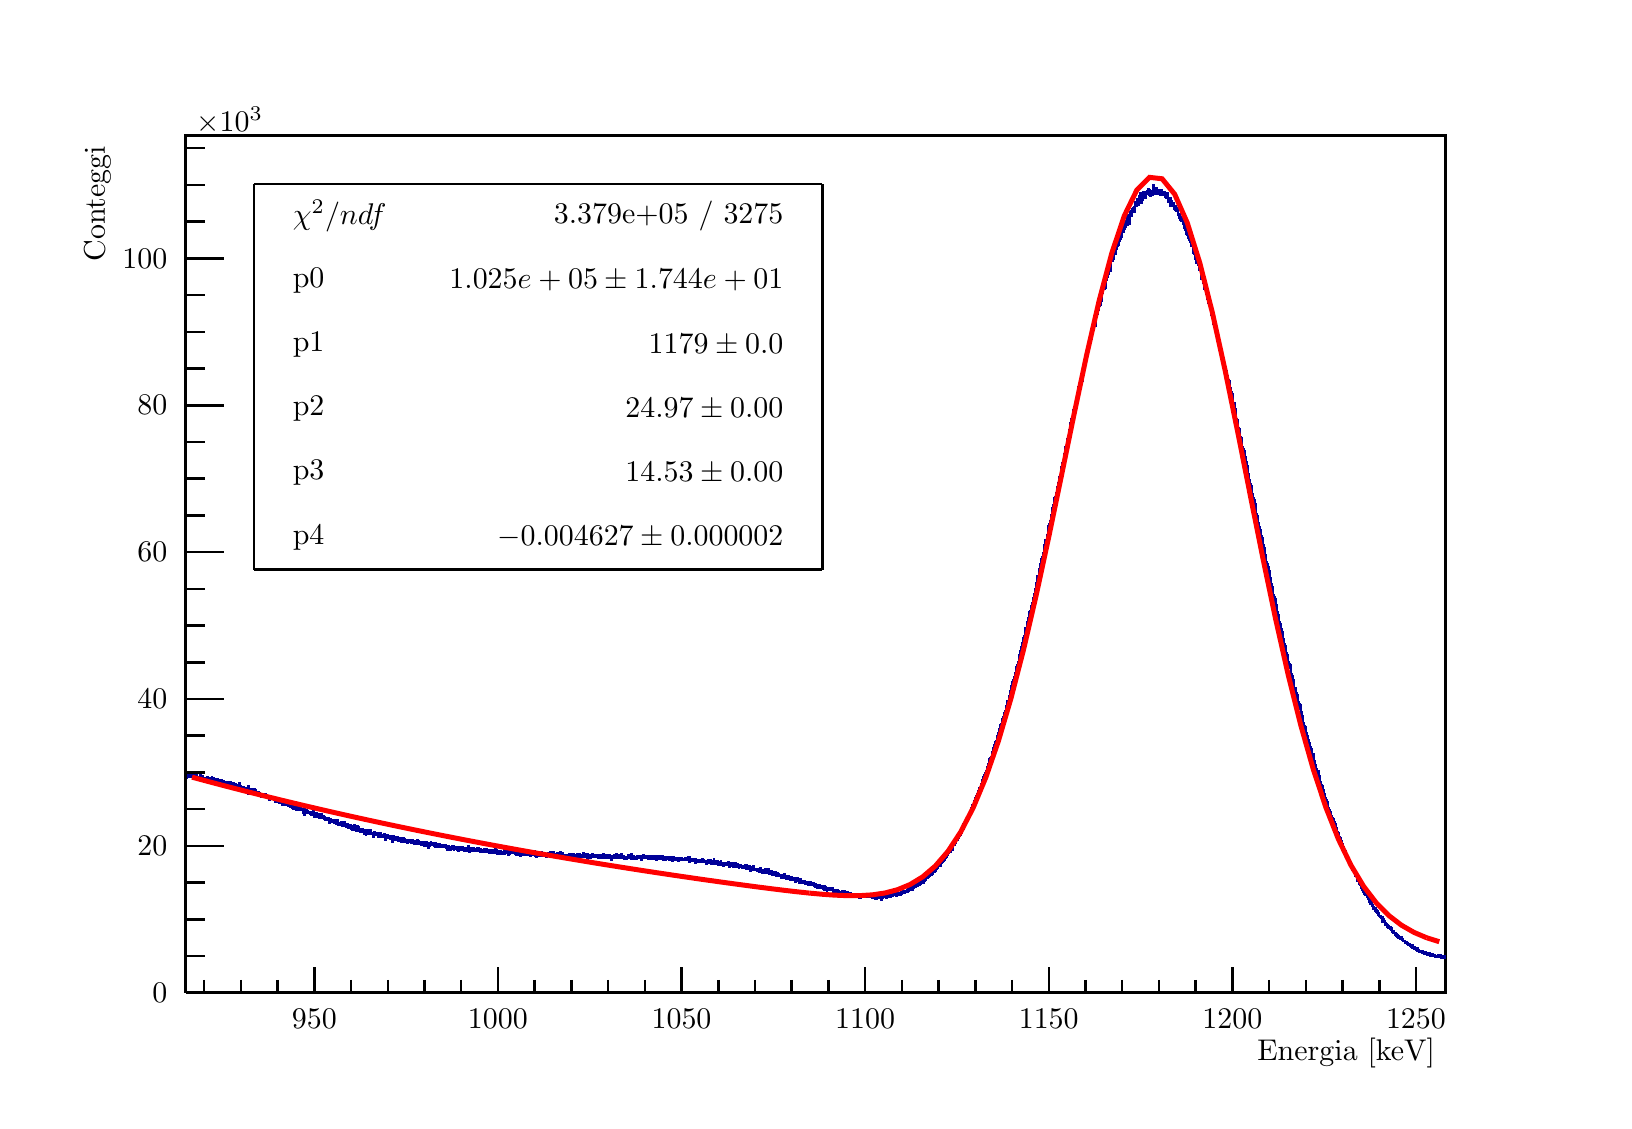
\begin{tikzpicture}
\pgfdeclareplotmark{cross} {
\pgfpathmoveto{\pgfpoint{-0.3\pgfplotmarksize}{\pgfplotmarksize}}
\pgfpathlineto{\pgfpoint{+0.3\pgfplotmarksize}{\pgfplotmarksize}}
\pgfpathlineto{\pgfpoint{+0.3\pgfplotmarksize}{0.3\pgfplotmarksize}}
\pgfpathlineto{\pgfpoint{+1\pgfplotmarksize}{0.3\pgfplotmarksize}}
\pgfpathlineto{\pgfpoint{+1\pgfplotmarksize}{-0.3\pgfplotmarksize}}
\pgfpathlineto{\pgfpoint{+0.3\pgfplotmarksize}{-0.3\pgfplotmarksize}}
\pgfpathlineto{\pgfpoint{+0.3\pgfplotmarksize}{-1.\pgfplotmarksize}}
\pgfpathlineto{\pgfpoint{-0.3\pgfplotmarksize}{-1.\pgfplotmarksize}}
\pgfpathlineto{\pgfpoint{-0.3\pgfplotmarksize}{-0.3\pgfplotmarksize}}
\pgfpathlineto{\pgfpoint{-1.\pgfplotmarksize}{-0.3\pgfplotmarksize}}
\pgfpathlineto{\pgfpoint{-1.\pgfplotmarksize}{0.3\pgfplotmarksize}}
\pgfpathlineto{\pgfpoint{-0.3\pgfplotmarksize}{0.3\pgfplotmarksize}}
\pgfpathclose
\pgfusepathqstroke
}
\pgfdeclareplotmark{cross*} {
\pgfpathmoveto{\pgfpoint{-0.3\pgfplotmarksize}{\pgfplotmarksize}}
\pgfpathlineto{\pgfpoint{+0.3\pgfplotmarksize}{\pgfplotmarksize}}
\pgfpathlineto{\pgfpoint{+0.3\pgfplotmarksize}{0.3\pgfplotmarksize}}
\pgfpathlineto{\pgfpoint{+1\pgfplotmarksize}{0.3\pgfplotmarksize}}
\pgfpathlineto{\pgfpoint{+1\pgfplotmarksize}{-0.3\pgfplotmarksize}}
\pgfpathlineto{\pgfpoint{+0.3\pgfplotmarksize}{-0.3\pgfplotmarksize}}
\pgfpathlineto{\pgfpoint{+0.3\pgfplotmarksize}{-1.\pgfplotmarksize}}
\pgfpathlineto{\pgfpoint{-0.3\pgfplotmarksize}{-1.\pgfplotmarksize}}
\pgfpathlineto{\pgfpoint{-0.3\pgfplotmarksize}{-0.3\pgfplotmarksize}}
\pgfpathlineto{\pgfpoint{-1.\pgfplotmarksize}{-0.3\pgfplotmarksize}}
\pgfpathlineto{\pgfpoint{-1.\pgfplotmarksize}{0.3\pgfplotmarksize}}
\pgfpathlineto{\pgfpoint{-0.3\pgfplotmarksize}{0.3\pgfplotmarksize}}
\pgfpathclose
\pgfusepathqfillstroke
}
\pgfdeclareplotmark{newstar} {
\pgfpathmoveto{\pgfqpoint{0pt}{\pgfplotmarksize}}
\pgfpathlineto{\pgfqpointpolar{44}{0.5\pgfplotmarksize}}
\pgfpathlineto{\pgfqpointpolar{18}{\pgfplotmarksize}}
\pgfpathlineto{\pgfqpointpolar{-20}{0.5\pgfplotmarksize}}
\pgfpathlineto{\pgfqpointpolar{-54}{\pgfplotmarksize}}
\pgfpathlineto{\pgfqpointpolar{-90}{0.5\pgfplotmarksize}}
\pgfpathlineto{\pgfqpointpolar{234}{\pgfplotmarksize}}
\pgfpathlineto{\pgfqpointpolar{198}{0.5\pgfplotmarksize}}
\pgfpathlineto{\pgfqpointpolar{162}{\pgfplotmarksize}}
\pgfpathlineto{\pgfqpointpolar{134}{0.5\pgfplotmarksize}}
\pgfpathclose
\pgfusepathqstroke
}
\pgfdeclareplotmark{newstar*} {
\pgfpathmoveto{\pgfqpoint{0pt}{\pgfplotmarksize}}
\pgfpathlineto{\pgfqpointpolar{44}{0.5\pgfplotmarksize}}
\pgfpathlineto{\pgfqpointpolar{18}{\pgfplotmarksize}}
\pgfpathlineto{\pgfqpointpolar{-20}{0.5\pgfplotmarksize}}
\pgfpathlineto{\pgfqpointpolar{-54}{\pgfplotmarksize}}
\pgfpathlineto{\pgfqpointpolar{-90}{0.5\pgfplotmarksize}}
\pgfpathlineto{\pgfqpointpolar{234}{\pgfplotmarksize}}
\pgfpathlineto{\pgfqpointpolar{198}{0.5\pgfplotmarksize}}
\pgfpathlineto{\pgfqpointpolar{162}{\pgfplotmarksize}}
\pgfpathlineto{\pgfqpointpolar{134}{0.5\pgfplotmarksize}}
\pgfpathclose
\pgfusepathqfillstroke
}
\definecolor{c}{rgb}{1,1,1};
\draw [color=c, fill=c] (0,0) rectangle (20,13.6103);
\draw [color=c, fill=c] (2,1.36103) rectangle (18,12.2493);
\definecolor{c}{rgb}{0,0,0};
\draw [c,line width=0.9] (2,1.36103) -- (2,12.2493) -- (18,12.2493) -- (18,1.36103) -- (2,1.36103);
\definecolor{c}{rgb}{1,1,1};
\draw [color=c, fill=c] (2,1.36103) rectangle (18,12.2493);
\definecolor{c}{rgb}{0,0,0};
\draw [c,line width=0.9] (2,1.36103) -- (2,12.2493) -- (18,12.2493) -- (18,1.36103) -- (2,1.36103);
\definecolor{c}{rgb}{0,0,0.6};
\draw [c,line width=0.9] (2,4.11668) -- (2.00488,4.11668) -- (2.00488,4.13748) -- (2.00976,4.13748) -- (2.00976,4.09411) -- (2.01463,4.09411) -- (2.01463,4.1289) -- (2.01951,4.1289) -- (2.01951,4.10353) -- (2.02439,4.10353) -- (2.02439,4.10885) --
 (2.02927,4.10885) -- (2.02927,4.13366) -- (2.03415,4.13366) -- (2.03415,4.11314) -- (2.03902,4.11314) -- (2.03902,4.13776) -- (2.0439,4.13776) -- (2.0439,4.14811) -- (2.04878,4.14811) -- (2.04878,4.12881) -- (2.05366,4.12881) -- (2.05366,4.12797) --
 (2.05854,4.12797) -- (2.05854,4.0985) -- (2.06341,4.0985) -- (2.06341,4.11118) -- (2.06829,4.11118) -- (2.06829,4.12256) -- (2.07317,4.12256) -- (2.07317,4.11799) -- (2.07805,4.11799) -- (2.07805,4.09915) -- (2.08293,4.09915) -- (2.08293,4.12004) --
 (2.08781,4.12004) -- (2.08781,4.09906) -- (2.09268,4.09906) -- (2.09268,4.12125) -- (2.09756,4.12125) -- (2.09756,4.11323) -- (2.10244,4.11323) -- (2.10244,4.1012) -- (2.10732,4.1012) -- (2.10732,4.10512) -- (2.1122,4.10512) -- (2.1122,4.0847) --
 (2.11707,4.0847) -- (2.11707,4.12125) -- (2.12195,4.12125) -- (2.12195,4.09999) -- (2.12683,4.09999) -- (2.12683,4.09122) -- (2.13171,4.09122) -- (2.13171,4.11183) -- (2.13659,4.11183) -- (2.13659,4.11109) -- (2.14146,4.11109) -- (2.14146,4.12041)
 -- (2.14634,4.12041) -- (2.14634,4.10288) -- (2.15122,4.10288) -- (2.15122,4.10213) -- (2.1561,4.10213) -- (2.1561,4.08824) -- (2.16098,4.08824) -- (2.16098,4.1026) -- (2.16585,4.1026) -- (2.16585,4.09663) -- (2.17073,4.09663) -- (2.17073,4.09197)
 -- (2.17561,4.09197) -- (2.17561,4.08982) -- (2.18049,4.08982) -- (2.18049,4.08339) -- (2.18537,4.08339) -- (2.18537,4.13039) -- (2.19024,4.13039) -- (2.19024,4.08973) -- (2.19512,4.08973) -- (2.19512,4.09514) -- (2.2,4.09514) -- (2.2,4.1054) --
 (2.20488,4.1054) -- (2.20488,4.09626) -- (2.20976,4.09626) -- (2.20976,4.09085) -- (2.21463,4.09085) -- (2.21463,4.11566) -- (2.21951,4.11566) -- (2.21951,4.07369) -- (2.22439,4.07369) -- (2.22439,4.07481) -- (2.22927,4.07481) -- (2.22927,4.08721)
 -- (2.23415,4.08721) -- (2.23415,4.06837) -- (2.23902,4.06837) -- (2.23902,4.06222) -- (2.2439,4.06222) -- (2.2439,4.08069) -- (2.24878,4.08069) -- (2.24878,4.08619) -- (2.25366,4.08619) -- (2.25366,4.07416) -- (2.25854,4.07416) -- (2.25854,4.07472)
 -- (2.26341,4.07472) -- (2.26341,4.07173) -- (2.26829,4.07173) -- (2.26829,4.07266) -- (2.27317,4.07266) -- (2.27317,4.09617) -- (2.27805,4.09617) -- (2.27805,4.07957) -- (2.28293,4.07957) -- (2.28293,4.06558) -- (2.28781,4.06558) --
 (2.28781,4.09048) -- (2.29268,4.09048) -- (2.29268,4.07556) -- (2.29756,4.07556) -- (2.29756,4.09029) -- (2.30244,4.09029) -- (2.30244,4.07024) -- (2.30732,4.07024) -- (2.30732,4.07052) -- (2.3122,4.07052) -- (2.3122,4.07127) -- (2.31707,4.07127) --
 (2.31707,4.06576) -- (2.32195,4.06576) -- (2.32195,4.06026) -- (2.32683,4.06026) -- (2.32683,4.05299) -- (2.33171,4.05299) -- (2.33171,4.10176) -- (2.33659,4.10176) -- (2.33659,4.05289) -- (2.34146,4.05289) -- (2.34146,4.07136) -- (2.34634,4.07136)
 -- (2.34634,4.08171) -- (2.35122,4.08171) -- (2.35122,4.07621) -- (2.3561,4.07621) -- (2.3561,4.05877) -- (2.36098,4.05877) -- (2.36098,4.05718) -- (2.36585,4.05718) -- (2.36585,4.02967) -- (2.37073,4.02967) -- (2.37073,4.04627) -- (2.37561,4.04627)
 -- (2.37561,4.06381) -- (2.38049,4.06381) -- (2.38049,4.07537) -- (2.38537,4.07537) -- (2.38537,4.03797) -- (2.39024,4.03797) -- (2.39024,4.07015) -- (2.39512,4.07015) -- (2.39512,4.04702) -- (2.4,4.04702) -- (2.4,4.05467) -- (2.40488,4.05467) --
 (2.40488,4.07472) -- (2.40976,4.07472) -- (2.40976,4.03639) -- (2.41463,4.03639) -- (2.41463,4.04627) -- (2.41951,4.04627) -- (2.41951,4.03704) -- (2.42439,4.03704) -- (2.42439,4.05858) -- (2.42927,4.05858) -- (2.42927,4.0362) -- (2.43415,4.0362) --
 (2.43415,4.04926) -- (2.43902,4.04926) -- (2.43902,4.03853) -- (2.4439,4.03853) -- (2.4439,4.0196) -- (2.44878,4.0196) -- (2.44878,4.03499) -- (2.45366,4.03499) -- (2.45366,4.02566) -- (2.45854,4.02566) -- (2.45854,4.05933) -- (2.46341,4.05933) --
 (2.46341,4.00962) -- (2.46829,4.00962) -- (2.46829,4.01261) -- (2.47317,4.01261) -- (2.47317,4.04142) -- (2.47805,4.04142) -- (2.47805,4.0224) -- (2.48293,4.0224) -- (2.48293,4.03573) -- (2.4878,4.03573) -- (2.4878,4.02128) -- (2.49268,4.02128) --
 (2.49268,4.0389) -- (2.49756,4.0389) -- (2.49756,4.03816) -- (2.50244,4.03816) -- (2.50244,4.02977) -- (2.50732,4.02977) -- (2.50732,3.9947) -- (2.5122,3.9947) -- (2.5122,4.0044) -- (2.51707,4.0044) -- (2.51707,4.01251) -- (2.52195,4.01251) --
 (2.52195,4.01829) -- (2.52683,4.01829) -- (2.52683,4.00449) -- (2.53171,4.00449) -- (2.53171,4.01456) -- (2.53659,4.01456) -- (2.53659,4.03079) -- (2.54146,4.03079) -- (2.54146,4.00011) -- (2.54634,4.00011) -- (2.54634,3.9808) -- (2.55122,3.9808) --
 (2.55122,4.00776) -- (2.5561,4.00776) -- (2.5561,3.98146) -- (2.56098,3.98146) -- (2.56098,4.00132) -- (2.56585,4.00132) -- (2.56585,4.03723) -- (2.57073,4.03723) -- (2.57073,4.0238) -- (2.57561,4.0238) -- (2.57561,4.00841) -- (2.58049,4.00841) --
 (2.58049,4.00085) -- (2.58537,4.00085) -- (2.58537,4.0072) -- (2.59024,4.0072) -- (2.59024,3.99899) -- (2.59512,3.99899) -- (2.59512,4.0127) -- (2.6,4.0127) -- (2.6,4.02697) -- (2.60488,4.02697) -- (2.60488,3.9643) -- (2.60976,3.9643) --
 (2.60976,4.0182) -- (2.61463,4.0182) -- (2.61463,4.01438) -- (2.61951,4.01438) -- (2.61951,3.98929) -- (2.62439,3.98929) -- (2.62439,3.97567) -- (2.62927,3.97567) -- (2.62927,4.01251) -- (2.63415,4.01251) -- (2.63415,4.00524) -- (2.63902,4.00524) --
 (2.63902,3.98696) -- (2.6439,3.98696) -- (2.6439,3.99666) -- (2.64878,3.99666) -- (2.64878,3.96663) -- (2.65366,3.96663) -- (2.65366,3.97978) -- (2.65854,3.97978) -- (2.65854,3.9961) -- (2.66341,3.9961) -- (2.66341,3.94928) -- (2.66829,3.94928) --
 (2.66829,3.97334) -- (2.67317,3.97334) -- (2.67317,3.96196) -- (2.67805,3.96196) -- (2.67805,4.02594) -- (2.68293,4.02594) -- (2.68293,3.96915) -- (2.6878,3.96915) -- (2.6878,3.94453) -- (2.69268,3.94453) -- (2.69268,3.95889) -- (2.69756,3.95889) --
 (2.69756,3.98062) -- (2.70244,3.98062) -- (2.70244,3.96625) -- (2.70732,3.96625) -- (2.70732,3.9476) -- (2.7122,3.9476) -- (2.7122,3.96859) -- (2.71707,3.96859) -- (2.71707,3.9684) -- (2.72195,3.9684) -- (2.72195,3.94863) -- (2.72683,3.94863) --
 (2.72683,3.97166) -- (2.73171,3.97166) -- (2.73171,3.94695) -- (2.73659,3.94695) -- (2.73659,3.97176) -- (2.74146,3.97176) -- (2.74146,3.92662) -- (2.74634,3.92662) -- (2.74634,3.93846) -- (2.75122,3.93846) -- (2.75122,3.96038) -- (2.7561,3.96038)
 -- (2.7561,3.94042) -- (2.76098,3.94042) -- (2.76098,3.93996) -- (2.76585,3.93996) -- (2.76585,3.96392) -- (2.77073,3.96392) -- (2.77073,3.94061) -- (2.77561,3.94061) -- (2.77561,3.95115) -- (2.78049,3.95115) -- (2.78049,3.92) -- (2.78537,3.92) --
 (2.78537,3.94658) -- (2.79024,3.94658) -- (2.79024,3.98332) -- (2.79512,3.98332) -- (2.79512,3.89416) -- (2.8,3.89416) -- (2.8,3.95292) -- (2.80488,3.95292) -- (2.80488,3.94891) -- (2.80976,3.94891) -- (2.80976,3.92438) -- (2.81463,3.92438) --
 (2.81463,3.90703) -- (2.81951,3.90703) -- (2.81951,3.94369) -- (2.82439,3.94369) -- (2.82439,3.94331) -- (2.82927,3.94331) -- (2.82927,3.93044) -- (2.83415,3.93044) -- (2.83415,3.94024) -- (2.83902,3.94024) -- (2.83902,3.92336) -- (2.8439,3.92336)
 -- (2.8439,3.9283) -- (2.84878,3.9283) -- (2.84878,3.89454) -- (2.85366,3.89454) -- (2.85366,3.93166) -- (2.85854,3.93166) -- (2.85854,3.90759) -- (2.86341,3.90759) -- (2.86341,3.90172) -- (2.86829,3.90172) -- (2.86829,3.94984) -- (2.87317,3.94984)
 -- (2.87317,3.9117) -- (2.87805,3.9117) -- (2.87805,3.91356) -- (2.88293,3.91356) -- (2.88293,3.90246) -- (2.8878,3.90246) -- (2.8878,3.92876) -- (2.89268,3.92876) -- (2.89268,3.87803) -- (2.89756,3.87803) -- (2.89756,3.89799) -- (2.90244,3.89799)
 -- (2.90244,3.89165) -- (2.90732,3.89165) -- (2.90732,3.89668) -- (2.9122,3.89668) -- (2.9122,3.88652) -- (2.91707,3.88652) -- (2.91707,3.89985) -- (2.92195,3.89985) -- (2.92195,3.90909) -- (2.92683,3.90909) -- (2.92683,3.88344) -- (2.93171,3.88344)
 -- (2.93171,3.884) -- (2.93659,3.884) -- (2.93659,3.87122) -- (2.94146,3.87122) -- (2.94146,3.89528) -- (2.94634,3.89528) -- (2.94634,3.87225) -- (2.95122,3.87225) -- (2.95122,3.86917) -- (2.9561,3.86917) -- (2.9561,3.86581) -- (2.96098,3.86581) --
 (2.96098,3.84586) -- (2.96585,3.84586) -- (2.96585,3.84418) -- (2.97073,3.84418) -- (2.97073,3.86208) -- (2.97561,3.86208) -- (2.97561,3.86292) -- (2.98049,3.86292) -- (2.98049,3.87775) -- (2.98537,3.87775) -- (2.98537,3.86954) -- (2.99024,3.86954)
 -- (2.99024,3.85528) -- (2.99512,3.85528) -- (2.99512,3.86721) -- (3,3.86721) -- (3,3.87505) -- (3.00488,3.87505) -- (3.00488,3.8812) -- (3.00976,3.8812) -- (3.00976,3.87439) -- (3.01463,3.87439) -- (3.01463,3.88111) -- (3.01951,3.88111) --
 (3.01951,3.86068) -- (3.02439,3.86068) -- (3.02439,3.85304) -- (3.02927,3.85304) -- (3.02927,3.8494) -- (3.03415,3.8494) -- (3.03415,3.83308) -- (3.03902,3.83308) -- (3.03902,3.84539) -- (3.0439,3.84539) -- (3.0439,3.84623) -- (3.04878,3.84623) --
 (3.04878,3.83606) -- (3.05366,3.83606) -- (3.05366,3.84511) -- (3.05854,3.84511) -- (3.05854,3.8467) -- (3.06341,3.8467) -- (3.06341,3.81452) -- (3.06829,3.81452) -- (3.06829,3.82608) -- (3.07317,3.82608) -- (3.07317,3.82422) -- (3.07805,3.82422) --
 (3.07805,3.82469) -- (3.08293,3.82469) -- (3.08293,3.84278) -- (3.08781,3.84278) -- (3.08781,3.82972) -- (3.09268,3.82972) -- (3.09268,3.82133) -- (3.09756,3.82133) -- (3.09756,3.8259) -- (3.10244,3.8259) -- (3.10244,3.83606) -- (3.10732,3.83606) --
 (3.10732,3.83121) -- (3.1122,3.83121) -- (3.1122,3.82506) -- (3.11707,3.82506) -- (3.11707,3.8245) -- (3.12195,3.8245) -- (3.12195,3.81172) -- (3.12683,3.81172) -- (3.12683,3.83979) -- (3.13171,3.83979) -- (3.13171,3.8009) -- (3.13659,3.8009) --
 (3.13659,3.82235) -- (3.14146,3.82235) -- (3.14146,3.79242) -- (3.14634,3.79242) -- (3.14634,3.79512) -- (3.15122,3.79512) -- (3.15122,3.82198) -- (3.1561,3.82198) -- (3.1561,3.81685) -- (3.16098,3.81685) -- (3.16098,3.80734) -- (3.16585,3.80734) --
 (3.16585,3.79494) -- (3.17073,3.79494) -- (3.17073,3.80109) -- (3.17561,3.80109) -- (3.17561,3.79195) -- (3.18049,3.79195) -- (3.18049,3.78729) -- (3.18537,3.78729) -- (3.18537,3.80016) -- (3.19024,3.80016) -- (3.19024,3.77871) -- (3.19512,3.77871)
 -- (3.19512,3.77087) -- (3.2,3.77087) -- (3.2,3.79335) -- (3.20488,3.79335) -- (3.20488,3.77022) -- (3.20976,3.77022) -- (3.20976,3.7678) -- (3.21463,3.7678) -- (3.21463,3.80473) -- (3.21951,3.80473) -- (3.21951,3.76985) -- (3.22439,3.76985) --
 (3.22439,3.74541) -- (3.22927,3.74541) -- (3.22927,3.77293) -- (3.23415,3.77293) -- (3.23415,3.80408) -- (3.23902,3.80408) -- (3.23902,3.76491) -- (3.2439,3.76491) -- (3.2439,3.7512) -- (3.24878,3.7512) -- (3.24878,3.76836) -- (3.25366,3.76836) --
 (3.25366,3.78757) -- (3.25854,3.78757) -- (3.25854,3.75539) -- (3.26341,3.75539) -- (3.26341,3.76463) -- (3.26829,3.76463) -- (3.26829,3.76547) -- (3.27317,3.76547) -- (3.27317,3.75791) -- (3.27805,3.75791) -- (3.27805,3.78076) -- (3.28293,3.78076)
 -- (3.28293,3.74411) -- (3.28781,3.74411) -- (3.28781,3.75073) -- (3.29268,3.75073) -- (3.29268,3.76491) -- (3.29756,3.76491) -- (3.29756,3.73469) -- (3.30244,3.73469) -- (3.30244,3.76127) -- (3.30732,3.76127) -- (3.30732,3.76584) --
 (3.3122,3.76584) -- (3.3122,3.74448) -- (3.31707,3.74448) -- (3.31707,3.75073) -- (3.32195,3.75073) -- (3.32195,3.7332) -- (3.32683,3.7332) -- (3.32683,3.72779) -- (3.33171,3.72779) -- (3.33171,3.75763) -- (3.33659,3.75763) -- (3.33659,3.73693) --
 (3.34146,3.73693) -- (3.34146,3.73898) -- (3.34634,3.73898) -- (3.34634,3.7373) -- (3.35122,3.7373) -- (3.35122,3.71445) -- (3.3561,3.71445) -- (3.3561,3.73059) -- (3.36098,3.73059) -- (3.36098,3.72583) -- (3.36585,3.72583) -- (3.36585,3.74075) --
 (3.37073,3.74075) -- (3.37073,3.69188) -- (3.37561,3.69188) -- (3.37561,3.74569) -- (3.38049,3.74569) -- (3.38049,3.72611) -- (3.38537,3.72611) -- (3.38537,3.70531) -- (3.39024,3.70531) -- (3.39024,3.718) -- (3.39512,3.718) -- (3.39512,3.70513) --
 (3.4,3.70513) -- (3.4,3.68657) -- (3.40488,3.68657) -- (3.40488,3.70792) -- (3.40976,3.70792) -- (3.40976,3.70037) -- (3.41463,3.70037) -- (3.41463,3.70345) -- (3.41951,3.70345) -- (3.41951,3.71371) -- (3.42439,3.71371) -- (3.42439,3.71035) --
 (3.42927,3.71035) -- (3.42927,3.71511) -- (3.43415,3.71511) -- (3.43415,3.70354) -- (3.43902,3.70354) -- (3.43902,3.70289) -- (3.4439,3.70289) -- (3.4439,3.68685) -- (3.44878,3.68685) -- (3.44878,3.69207) -- (3.45366,3.69207) -- (3.45366,3.70112) --
 (3.45854,3.70112) -- (3.45854,3.70886) -- (3.46341,3.70886) -- (3.46341,3.68424) -- (3.46829,3.68424) -- (3.46829,3.67929) -- (3.47317,3.67929) -- (3.47317,3.68778) -- (3.47805,3.68778) -- (3.47805,3.68806) -- (3.48293,3.68806) -- (3.48293,3.68582)
 -- (3.4878,3.68582) -- (3.4878,3.69767) -- (3.49268,3.69767) -- (3.49268,3.64581) -- (3.49756,3.64581) -- (3.49756,3.65533) -- (3.50244,3.65533) -- (3.50244,3.68834) -- (3.50732,3.68834) -- (3.50732,3.62455) -- (3.5122,3.62455) -- (3.5122,3.67929)
 -- (3.51707,3.67929) -- (3.51707,3.65999) -- (3.52195,3.65999) -- (3.52195,3.67808) -- (3.52683,3.67808) -- (3.52683,3.67939) -- (3.53171,3.67939) -- (3.53171,3.66223) -- (3.53659,3.66223) -- (3.53659,3.6487) -- (3.54146,3.6487) -- (3.54146,3.67183)
 -- (3.54634,3.67183) -- (3.54634,3.66698) -- (3.55122,3.66698) -- (3.55122,3.65318) -- (3.5561,3.65318) -- (3.5561,3.65924) -- (3.56098,3.65924) -- (3.56098,3.64096) -- (3.56585,3.64096) -- (3.56585,3.65495) -- (3.57073,3.65495) -- (3.57073,3.65038)
 -- (3.57561,3.65038) -- (3.57561,3.65234) -- (3.58049,3.65234) -- (3.58049,3.63369) -- (3.58537,3.63369) -- (3.58537,3.64404) -- (3.59024,3.64404) -- (3.59024,3.63956) -- (3.59512,3.63956) -- (3.59512,3.65766) -- (3.6,3.65766) -- (3.6,3.62194) --
 (3.60488,3.62194) -- (3.60488,3.62884) -- (3.60976,3.62884) -- (3.60976,3.63341) -- (3.61463,3.63341) -- (3.61463,3.61858) -- (3.61951,3.61858) -- (3.61951,3.66381) -- (3.62439,3.66381) -- (3.62439,3.6709) -- (3.62927,3.6709) -- (3.62927,3.63145) --
 (3.63415,3.63145) -- (3.63415,3.59862) -- (3.63902,3.59862) -- (3.63902,3.62511) -- (3.6439,3.62511) -- (3.6439,3.61821) -- (3.64878,3.61821) -- (3.64878,3.60021) -- (3.65366,3.60021) -- (3.65366,3.63509) -- (3.65854,3.63509) -- (3.65854,3.60245) --
 (3.66341,3.60245) -- (3.66341,3.63033) -- (3.66829,3.63033) -- (3.66829,3.6017) -- (3.67317,3.6017) -- (3.67317,3.62296) -- (3.67805,3.62296) -- (3.67805,3.60375) -- (3.68293,3.60375) -- (3.68293,3.62436) -- (3.6878,3.62436) -- (3.6878,3.6004) --
 (3.69268,3.6004) -- (3.69268,3.60832) -- (3.69756,3.60832) -- (3.69756,3.58892) -- (3.70244,3.58892) -- (3.70244,3.59965) -- (3.70732,3.59965) -- (3.70732,3.58976) -- (3.7122,3.58976) -- (3.7122,3.6114) -- (3.71707,3.6114) -- (3.71707,3.59144) --
 (3.72195,3.59144) -- (3.72195,3.59098) -- (3.72683,3.59098) -- (3.72683,3.62343) -- (3.73171,3.62343) -- (3.73171,3.58445) -- (3.73659,3.58445) -- (3.73659,3.58109) -- (3.74146,3.58109) -- (3.74146,3.58296) -- (3.74634,3.58296) -- (3.74634,3.60599)
 -- (3.75122,3.60599) -- (3.75122,3.60692) -- (3.7561,3.60692) -- (3.7561,3.59433) -- (3.76098,3.59433) -- (3.76098,3.56878) -- (3.76585,3.56878) -- (3.76585,3.55218) -- (3.77073,3.55218) -- (3.77073,3.5575) -- (3.77561,3.5575) -- (3.77561,3.56785)
 -- (3.78049,3.56785) -- (3.78049,3.56281) -- (3.78537,3.56281) -- (3.78537,3.56831) -- (3.79024,3.56831) -- (3.79024,3.57633) -- (3.79512,3.57633) -- (3.79512,3.56701) -- (3.8,3.56701) -- (3.8,3.56225) -- (3.80488,3.56225) -- (3.80488,3.55852) --
 (3.80976,3.55852) -- (3.80976,3.56244) -- (3.81463,3.56244) -- (3.81463,3.57111) -- (3.81951,3.57111) -- (3.81951,3.56067) -- (3.82439,3.56067) -- (3.82439,3.52364) -- (3.82927,3.52364) -- (3.82927,3.54519) -- (3.83415,3.54519) -- (3.83415,3.53465)
 -- (3.83902,3.53465) -- (3.83902,3.5685) -- (3.8439,3.5685) -- (3.8439,3.54416) -- (3.84878,3.54416) -- (3.84878,3.53875) -- (3.85366,3.53875) -- (3.85366,3.53241) -- (3.85854,3.53241) -- (3.85854,3.53633) -- (3.86341,3.53633) -- (3.86341,3.55125)
 -- (3.86829,3.55125) -- (3.86829,3.52868) -- (3.87317,3.52868) -- (3.87317,3.53847) -- (3.87805,3.53847) -- (3.87805,3.53446) -- (3.88293,3.53446) -- (3.88293,3.53744) -- (3.8878,3.53744) -- (3.8878,3.52178) -- (3.89268,3.52178) -- (3.89268,3.53511)
 -- (3.89756,3.53511) -- (3.89756,3.5477) -- (3.90244,3.5477) -- (3.90244,3.55731) -- (3.90732,3.55731) -- (3.90732,3.53866) -- (3.9122,3.53866) -- (3.9122,3.50993) -- (3.91707,3.50993) -- (3.91707,3.5049) -- (3.92195,3.5049) -- (3.92195,3.53558) --
 (3.92683,3.53558) -- (3.92683,3.55237) -- (3.93171,3.55237) -- (3.93171,3.52467) -- (3.93659,3.52467) -- (3.93659,3.50061) -- (3.94146,3.50061) -- (3.94146,3.51935) -- (3.94634,3.51935) -- (3.94634,3.49716) -- (3.95122,3.49716) -- (3.95122,3.51441)
 -- (3.9561,3.51441) -- (3.9561,3.50993) -- (3.96098,3.50993) -- (3.96098,3.49772) -- (3.96585,3.49772) -- (3.96585,3.51376) -- (3.97073,3.51376) -- (3.97073,3.52485) -- (3.97561,3.52485) -- (3.97561,3.51861) -- (3.98049,3.51861) -- (3.98049,3.49977)
 -- (3.98537,3.49977) -- (3.98537,3.52635) -- (3.99024,3.52635) -- (3.99024,3.48429) -- (3.99512,3.48429) -- (3.99512,3.49874) -- (4,3.49874) -- (4,3.49883) -- (4.00488,3.49883) -- (4.00488,3.49231) -- (4.00976,3.49231) -- (4.00976,3.49566) --
 (4.01463,3.49566) -- (4.01463,3.49007) -- (4.01951,3.49007) -- (4.01951,3.52346) -- (4.02439,3.52346) -- (4.02439,3.50704) -- (4.02927,3.50704) -- (4.02927,3.47543) -- (4.03415,3.47543) -- (4.03415,3.46834) -- (4.03902,3.46834) -- (4.03902,3.46862)
 -- (4.0439,3.46862) -- (4.0439,3.48503) -- (4.04878,3.48503) -- (4.04878,3.49594) -- (4.05366,3.49594) -- (4.05366,3.4786) -- (4.05854,3.4786) -- (4.05854,3.45323) -- (4.06341,3.45323) -- (4.06341,3.47058) -- (4.06829,3.47058) -- (4.06829,3.473) --
 (4.07317,3.473) -- (4.07317,3.46097) -- (4.07805,3.46097) -- (4.07805,3.46638) -- (4.08293,3.46638) -- (4.08293,3.48214) -- (4.0878,3.48214) -- (4.0878,3.45761) -- (4.09268,3.45761) -- (4.09268,3.48391) -- (4.09756,3.48391) -- (4.09756,3.44838) --
 (4.10244,3.44838) -- (4.10244,3.46992) -- (4.10732,3.46992) -- (4.10732,3.45276) -- (4.1122,3.45276) -- (4.1122,3.46386) -- (4.11707,3.46386) -- (4.11707,3.43327) -- (4.12195,3.43327) -- (4.12195,3.47822) -- (4.12683,3.47822) -- (4.12683,3.4606) --
 (4.13171,3.4606) -- (4.13171,3.43327) -- (4.13659,3.43327) -- (4.13659,3.48186) -- (4.14146,3.48186) -- (4.14146,3.44763) -- (4.14634,3.44763) -- (4.14634,3.45556) -- (4.15122,3.45556) -- (4.15122,3.44885) -- (4.1561,3.44885) -- (4.1561,3.45799) --
 (4.16098,3.45799) -- (4.16098,3.47972) -- (4.16585,3.47972) -- (4.16585,3.46274) -- (4.17073,3.46274) -- (4.17073,3.41509) -- (4.17561,3.41509) -- (4.17561,3.47207) -- (4.18049,3.47207) -- (4.18049,3.42796) -- (4.18537,3.42796) -- (4.18537,3.43672)
 -- (4.19024,3.43672) -- (4.19024,3.42964) -- (4.19512,3.42964) -- (4.19512,3.45939) -- (4.2,3.45939) -- (4.2,3.44325) -- (4.20488,3.44325) -- (4.20488,3.42078) -- (4.20976,3.42078) -- (4.20976,3.41695) -- (4.21463,3.41695) -- (4.21463,3.43225) --
 (4.21951,3.43225) -- (4.21951,3.40464) -- (4.22439,3.40464) -- (4.22439,3.4025) -- (4.22927,3.4025) -- (4.22927,3.42861) -- (4.23415,3.42861) -- (4.23415,3.42992) -- (4.23902,3.42992) -- (4.23902,3.4398) -- (4.2439,3.4398) -- (4.2439,3.40968) --
 (4.24878,3.40968) -- (4.24878,3.41257) -- (4.25366,3.41257) -- (4.25366,3.40996) -- (4.25854,3.40996) -- (4.25854,3.41527) -- (4.26341,3.41527) -- (4.26341,3.4219) -- (4.26829,3.4219) -- (4.26829,3.40819) -- (4.27317,3.40819) -- (4.27317,3.38319) --
 (4.27805,3.38319) -- (4.27805,3.4205) -- (4.28293,3.4205) -- (4.28293,3.41201) -- (4.28781,3.41201) -- (4.28781,3.36752) -- (4.29268,3.36752) -- (4.29268,3.41229) -- (4.29756,3.41229) -- (4.29756,3.40697) -- (4.30244,3.40697) -- (4.30244,3.401) --
 (4.30732,3.401) -- (4.30732,3.42106) -- (4.3122,3.42106) -- (4.3122,3.39205) -- (4.31707,3.39205) -- (4.31707,3.38217) -- (4.32195,3.38217) -- (4.32195,3.38021) -- (4.32683,3.38021) -- (4.32683,3.40007) -- (4.33171,3.40007) -- (4.33171,3.42712) --
 (4.33659,3.42712) -- (4.33659,3.40231) -- (4.34146,3.40231) -- (4.34146,3.38646) -- (4.34634,3.38646) -- (4.34634,3.42245) -- (4.35122,3.42245) -- (4.35122,3.4024) -- (4.3561,3.4024) -- (4.3561,3.38496) -- (4.36098,3.38496) -- (4.36098,3.3886) --
 (4.36585,3.3886) -- (4.36585,3.37517) -- (4.37073,3.37517) -- (4.37073,3.38795) -- (4.37561,3.38795) -- (4.37561,3.37265) -- (4.38049,3.37265) -- (4.38049,3.38459) -- (4.38537,3.38459) -- (4.38537,3.34505) -- (4.39024,3.34505) -- (4.39024,3.3997) --
 (4.39512,3.3997) -- (4.39512,3.37704) -- (4.4,3.37704) -- (4.4,3.39541) -- (4.40488,3.39541) -- (4.40488,3.39224) -- (4.40976,3.39224) -- (4.40976,3.36771) -- (4.41463,3.36771) -- (4.41463,3.3776) -- (4.41951,3.3776) -- (4.41951,3.38077) --
 (4.42439,3.38077) -- (4.42439,3.36379) -- (4.42927,3.36379) -- (4.42927,3.37825) -- (4.43415,3.37825) -- (4.43415,3.37004) -- (4.43902,3.37004) -- (4.43902,3.34141) -- (4.4439,3.34141) -- (4.4439,3.38049) -- (4.44878,3.38049) -- (4.44878,3.35615) --
 (4.45366,3.35615) -- (4.45366,3.33638) -- (4.45854,3.33638) -- (4.45854,3.38021) -- (4.46341,3.38021) -- (4.46341,3.35064) -- (4.46829,3.35064) -- (4.46829,3.38086) -- (4.47317,3.38086) -- (4.47317,3.35615) -- (4.47805,3.35615) -- (4.47805,3.34468)
 -- (4.48293,3.34468) -- (4.48293,3.3499) -- (4.4878,3.3499) -- (4.4878,3.36062) -- (4.49268,3.36062) -- (4.49268,3.35158) -- (4.49756,3.35158) -- (4.49756,3.34859) -- (4.50244,3.34859) -- (4.50244,3.34085) -- (4.50732,3.34085) -- (4.50732,3.34822)
 -- (4.5122,3.34822) -- (4.5122,3.3415) -- (4.51707,3.3415) -- (4.51707,3.33852) -- (4.52195,3.33852) -- (4.52195,3.36939) -- (4.52683,3.36939) -- (4.52683,3.35046) -- (4.53171,3.35046) -- (4.53171,3.30737) -- (4.53659,3.30737) -- (4.53659,3.3346) --
 (4.54146,3.3346) -- (4.54146,3.35503) -- (4.54634,3.35503) -- (4.54634,3.33209) -- (4.55122,3.33209) -- (4.55122,3.32975) -- (4.5561,3.32975) -- (4.5561,3.35969) -- (4.56098,3.35969) -- (4.56098,3.33759) -- (4.56585,3.33759) -- (4.56585,3.34234) --
 (4.57073,3.34234) -- (4.57073,3.34123) -- (4.57561,3.34123) -- (4.57561,3.35036) -- (4.58049,3.35036) -- (4.58049,3.33339) -- (4.58537,3.33339) -- (4.58537,3.34701) -- (4.59024,3.34701) -- (4.59024,3.35046) -- (4.59512,3.35046) -- (4.59512,3.3222)
 -- (4.6,3.3222) -- (4.6,3.34477) -- (4.60488,3.34477) -- (4.60488,3.34514) -- (4.60976,3.34514) -- (4.60976,3.32752) -- (4.61463,3.32752) -- (4.61463,3.3429) -- (4.61951,3.3429) -- (4.61951,3.33227) -- (4.62439,3.33227) -- (4.62439,3.28051) --
 (4.62927,3.28051) -- (4.62927,3.30411) -- (4.63415,3.30411) -- (4.63415,3.34384) -- (4.63902,3.34384) -- (4.63902,3.3291) -- (4.6439,3.3291) -- (4.6439,3.3277) -- (4.64878,3.3277) -- (4.64878,3.31987) -- (4.65366,3.31987) -- (4.65366,3.32752) --
 (4.65854,3.32752) -- (4.65854,3.29926) -- (4.66341,3.29926) -- (4.66341,3.3332) -- (4.66829,3.3332) -- (4.66829,3.31399) -- (4.67317,3.31399) -- (4.67317,3.30868) -- (4.67805,3.30868) -- (4.67805,3.30457) -- (4.68293,3.30457) -- (4.68293,3.33442) --
 (4.68781,3.33442) -- (4.68781,3.33199) -- (4.69268,3.33199) -- (4.69268,3.30467) -- (4.69756,3.30467) -- (4.69756,3.28639) -- (4.70244,3.28639) -- (4.70244,3.30084) -- (4.70732,3.30084) -- (4.70732,3.31203) -- (4.7122,3.31203) -- (4.7122,3.32052) --
 (4.71707,3.32052) -- (4.71707,3.3166) -- (4.72195,3.3166) -- (4.72195,3.31539) -- (4.72683,3.31539) -- (4.72683,3.29739) -- (4.73171,3.29739) -- (4.73171,3.30196) -- (4.73659,3.30196) -- (4.73659,3.30299) -- (4.74146,3.30299) -- (4.74146,3.28284) --
 (4.74634,3.28284) -- (4.74634,3.318) -- (4.75122,3.318) -- (4.75122,3.30746) -- (4.7561,3.30746) -- (4.7561,3.28191) -- (4.76098,3.28191) -- (4.76098,3.31064) -- (4.76585,3.31064) -- (4.76585,3.32136) -- (4.77073,3.32136) -- (4.77073,3.29991) --
 (4.77561,3.29991) -- (4.77561,3.30569) -- (4.78049,3.30569) -- (4.78049,3.31409) -- (4.78537,3.31409) -- (4.78537,3.28555) -- (4.79024,3.28555) -- (4.79024,3.28051) -- (4.79512,3.28051) -- (4.79512,3.28126) -- (4.8,3.28126) -- (4.8,3.29562) --
 (4.80488,3.29562) -- (4.80488,3.27939) -- (4.80976,3.27939) -- (4.80976,3.26876) -- (4.81463,3.26876) -- (4.81463,3.29665) -- (4.81951,3.29665) -- (4.81951,3.28685) -- (4.82439,3.28685) -- (4.82439,3.28583) -- (4.82927,3.28583) -- (4.82927,3.2737)
 -- (4.83415,3.2737) -- (4.83415,3.29646) -- (4.83902,3.29646) -- (4.83902,3.29404) -- (4.8439,3.29404) -- (4.8439,3.29618) -- (4.84878,3.29618) -- (4.84878,3.27259) -- (4.85366,3.27259) -- (4.85366,3.28574) -- (4.85854,3.28574) -- (4.85854,3.28182)
 -- (4.86341,3.28182) -- (4.86341,3.27445) -- (4.86829,3.27445) -- (4.86829,3.26904) -- (4.87317,3.26904) -- (4.87317,3.271) -- (4.87805,3.271) -- (4.87805,3.28909) -- (4.88293,3.28909) -- (4.88293,3.29385) -- (4.8878,3.29385) -- (4.8878,3.28098) --
 (4.89268,3.28098) -- (4.89268,3.26503) -- (4.89756,3.26503) -- (4.89756,3.24983) -- (4.90244,3.24983) -- (4.90244,3.27799) -- (4.90732,3.27799) -- (4.90732,3.2849) -- (4.9122,3.2849) -- (4.9122,3.26223) -- (4.91707,3.26223) -- (4.91707,3.25738) --
 (4.92195,3.25738) -- (4.92195,3.27855) -- (4.92683,3.27855) -- (4.92683,3.26457) -- (4.93171,3.26457) -- (4.93171,3.25216) -- (4.93659,3.25216) -- (4.93659,3.27324) -- (4.94146,3.27324) -- (4.94146,3.29217) -- (4.94634,3.29217) -- (4.94634,3.26056)
 -- (4.95122,3.26056) -- (4.95122,3.26895) -- (4.9561,3.26895) -- (4.9561,3.2807) -- (4.96098,3.2807) -- (4.96098,3.26886) -- (4.96585,3.26886) -- (4.96585,3.26335) -- (4.97073,3.26335) -- (4.97073,3.25813) -- (4.97561,3.25813) -- (4.97561,3.27259)
 -- (4.98049,3.27259) -- (4.98049,3.2517) -- (4.98537,3.2517) -- (4.98537,3.24815) -- (4.99024,3.24815) -- (4.99024,3.23659) -- (4.99512,3.23659) -- (4.99512,3.26046) -- (5,3.26046) -- (5,3.25543) -- (5.00488,3.25543) -- (5.00488,3.25944) --
 (5.00976,3.25944) -- (5.00976,3.25235) -- (5.01463,3.25235) -- (5.01463,3.23687) -- (5.01951,3.23687) -- (5.01951,3.27594) -- (5.02439,3.27594) -- (5.02439,3.25291) -- (5.02927,3.25291) -- (5.02927,3.23379) -- (5.03415,3.23379) -- (5.03415,3.2239)
 -- (5.03902,3.2239) -- (5.03902,3.27025) -- (5.0439,3.27025) -- (5.0439,3.23351) -- (5.04878,3.23351) -- (5.04878,3.24442) -- (5.05366,3.24442) -- (5.05366,3.25198) -- (5.05854,3.25198) -- (5.05854,3.27818) -- (5.06341,3.27818) -- (5.06341,3.24908)
 -- (5.06829,3.24908) -- (5.06829,3.24834) -- (5.07317,3.24834) -- (5.07317,3.25384) -- (5.07805,3.25384) -- (5.07805,3.20712) -- (5.08293,3.20712) -- (5.08293,3.25673) -- (5.0878,3.25673) -- (5.0878,3.24274) -- (5.09268,3.24274) -- (5.09268,3.25067)
 -- (5.09756,3.25067) -- (5.09756,3.2309) -- (5.10244,3.2309) -- (5.10244,3.25477) -- (5.10732,3.25477) -- (5.10732,3.25309) -- (5.1122,3.25309) -- (5.1122,3.26662) -- (5.11707,3.26662) -- (5.11707,3.24769) -- (5.12195,3.24769) -- (5.12195,3.25319)
 -- (5.12683,3.25319) -- (5.12683,3.2599) -- (5.13171,3.2599) -- (5.13171,3.23715) -- (5.13659,3.23715) -- (5.13659,3.26046) -- (5.14146,3.26046) -- (5.14146,3.23556) -- (5.14634,3.23556) -- (5.14634,3.2434) -- (5.15122,3.2434) -- (5.15122,3.23556)
 -- (5.1561,3.23556) -- (5.1561,3.23696) -- (5.16098,3.23696) -- (5.16098,3.23118) -- (5.16585,3.23118) -- (5.16585,3.21915) -- (5.17073,3.21915) -- (5.17073,3.25393) -- (5.17561,3.25393) -- (5.17561,3.22381) -- (5.18049,3.22381) -- (5.18049,3.20898)
 -- (5.18537,3.20898) -- (5.18537,3.23957) -- (5.19024,3.23957) -- (5.19024,3.22931) -- (5.19512,3.22931) -- (5.19512,3.23621) -- (5.2,3.23621) -- (5.2,3.21514) -- (5.20488,3.21514) -- (5.20488,3.24293) -- (5.20976,3.24293) -- (5.20976,3.22987) --
 (5.21463,3.22987) -- (5.21463,3.23342) -- (5.21951,3.23342) -- (5.21951,3.24433) -- (5.22439,3.24433) -- (5.22439,3.20945) -- (5.22927,3.20945) -- (5.22927,3.21187) -- (5.23415,3.21187) -- (5.23415,3.21337) -- (5.23902,3.21337) -- (5.23902,3.21057)
 -- (5.2439,3.21057) -- (5.2439,3.23668) -- (5.24878,3.23668) -- (5.24878,3.21738) -- (5.25366,3.21738) -- (5.25366,3.21299) -- (5.25854,3.21299) -- (5.25854,3.21113) -- (5.26341,3.21113) -- (5.26341,3.22689) -- (5.26829,3.22689) -- (5.26829,3.23286)
 -- (5.27317,3.23286) -- (5.27317,3.21859) -- (5.27805,3.21859) -- (5.27805,3.217) -- (5.28293,3.217) -- (5.28293,3.21887) -- (5.28781,3.21887) -- (5.28781,3.23025) -- (5.29268,3.23025) -- (5.29268,3.21113) -- (5.29756,3.21113) -- (5.29756,3.23127)
 -- (5.30244,3.23127) -- (5.30244,3.19956) -- (5.30732,3.19956) -- (5.30732,3.22288) -- (5.3122,3.22288) -- (5.3122,3.20786) -- (5.31707,3.20786) -- (5.31707,3.2059) -- (5.32195,3.2059) -- (5.32195,3.17793) -- (5.32683,3.17793) -- (5.32683,3.20908)
 -- (5.33171,3.20908) -- (5.33171,3.21047) -- (5.33659,3.21047) -- (5.33659,3.2157) -- (5.34146,3.2157) -- (5.34146,3.19574) -- (5.34634,3.19574) -- (5.34634,3.17737) -- (5.35122,3.17737) -- (5.35122,3.20833) -- (5.3561,3.20833) -- (5.3561,3.18613)
 -- (5.36098,3.18613) -- (5.36098,3.18203) -- (5.36585,3.18203) -- (5.36585,3.20796) -- (5.37073,3.20796) -- (5.37073,3.20404) -- (5.37561,3.20404) -- (5.37561,3.20665) -- (5.38049,3.20665) -- (5.38049,3.18865) -- (5.38537,3.18865) --
 (5.38537,3.21905) -- (5.39024,3.21905) -- (5.39024,3.22596) -- (5.39512,3.22596) -- (5.39512,3.19919) -- (5.4,3.19919) -- (5.4,3.21887) -- (5.40488,3.21887) -- (5.40488,3.17569) -- (5.40976,3.17569) -- (5.40976,3.18408) -- (5.41463,3.18408) --
 (5.41463,3.18781) -- (5.41951,3.18781) -- (5.41951,3.20618) -- (5.42439,3.20618) -- (5.42439,3.18819) -- (5.42927,3.18819) -- (5.42927,3.1921) -- (5.43415,3.1921) -- (5.43415,3.2004) -- (5.43902,3.2004) -- (5.43902,3.199) -- (5.4439,3.199) --
 (5.4439,3.18884) -- (5.44878,3.18884) -- (5.44878,3.19164) -- (5.45366,3.19164) -- (5.45366,3.18278) -- (5.45854,3.18278) -- (5.45854,3.16804) -- (5.46341,3.16804) -- (5.46341,3.20516) -- (5.46829,3.20516) -- (5.46829,3.19387) -- (5.47317,3.19387)
 -- (5.47317,3.17662) -- (5.47805,3.17662) -- (5.47805,3.19956) -- (5.48293,3.19956) -- (5.48293,3.21225) -- (5.4878,3.21225) -- (5.4878,3.1825) -- (5.49268,3.1825) -- (5.49268,3.2142) -- (5.49756,3.2142) -- (5.49756,3.19658) -- (5.50244,3.19658) --
 (5.50244,3.188) -- (5.50732,3.188) -- (5.50732,3.17541) -- (5.5122,3.17541) -- (5.5122,3.2143) -- (5.51707,3.2143) -- (5.51707,3.2018) -- (5.52195,3.2018) -- (5.52195,3.19033) -- (5.52683,3.19033) -- (5.52683,3.18016) -- (5.53171,3.18016) --
 (5.53171,3.16739) -- (5.53659,3.16739) -- (5.53659,3.16356) -- (5.54146,3.16356) -- (5.54146,3.1894) -- (5.54634,3.1894) -- (5.54634,3.18856) -- (5.55122,3.18856) -- (5.55122,3.19537) -- (5.5561,3.19537) -- (5.5561,3.16935) -- (5.56098,3.16935) --
 (5.56098,3.18613) -- (5.56585,3.18613) -- (5.56585,3.18501) -- (5.57073,3.18501) -- (5.57073,3.16991) -- (5.57561,3.16991) -- (5.57561,3.16459) -- (5.58049,3.16459) -- (5.58049,3.18128) -- (5.58537,3.18128) -- (5.58537,3.21607) -- (5.59024,3.21607)
 -- (5.59024,3.16813) -- (5.59512,3.16813) -- (5.59512,3.2129) -- (5.6,3.2129) -- (5.6,3.15657) -- (5.60488,3.15657) -- (5.60488,3.16888) -- (5.60976,3.16888) -- (5.60976,3.19397) -- (5.61463,3.19397) -- (5.61463,3.16412) -- (5.61951,3.16412) --
 (5.61951,3.18119) -- (5.62439,3.18119) -- (5.62439,3.19639) -- (5.62927,3.19639) -- (5.62927,3.17149) -- (5.63415,3.17149) -- (5.63415,3.16963) -- (5.63902,3.16963) -- (5.63902,3.17979) -- (5.6439,3.17979) -- (5.6439,3.18371) -- (5.64878,3.18371) --
 (5.64878,3.17755) -- (5.65366,3.17755) -- (5.65366,3.17494) -- (5.65854,3.17494) -- (5.65854,3.20217) -- (5.66341,3.20217) -- (5.66341,3.17289) -- (5.66829,3.17289) -- (5.66829,3.15909) -- (5.67317,3.15909) -- (5.67317,3.17914) -- (5.67805,3.17914)
 -- (5.67805,3.18352) -- (5.68293,3.18352) -- (5.68293,3.18166) -- (5.68781,3.18166) -- (5.68781,3.1769) -- (5.69268,3.1769) -- (5.69268,3.16366) -- (5.69756,3.16366) -- (5.69756,3.17103) -- (5.70244,3.17103) -- (5.70244,3.20012) -- (5.70732,3.20012)
 -- (5.70732,3.1714) -- (5.7122,3.1714) -- (5.7122,3.20208) -- (5.71707,3.20208) -- (5.71707,3.19285) -- (5.72195,3.19285) -- (5.72195,3.16142) -- (5.72683,3.16142) -- (5.72683,3.15965) -- (5.73171,3.15965) -- (5.73171,3.17569) -- (5.73659,3.17569)
 -- (5.73659,3.18371) -- (5.74146,3.18371) -- (5.74146,3.15237) -- (5.74634,3.15237) -- (5.74634,3.14976) -- (5.75122,3.14976) -- (5.75122,3.17037) -- (5.7561,3.17037) -- (5.7561,3.15918) -- (5.76098,3.15918) -- (5.76098,3.16795) -- (5.76585,3.16795)
 -- (5.76585,3.17326) -- (5.77073,3.17326) -- (5.77073,3.1534) -- (5.77561,3.1534) -- (5.77561,3.16095) -- (5.78049,3.16095) -- (5.78049,3.17093) -- (5.78537,3.17093) -- (5.78537,3.18436) -- (5.79024,3.18436) -- (5.79024,3.15275) -- (5.79512,3.15275)
 -- (5.79512,3.15918) -- (5.8,3.15918) -- (5.8,3.18688) -- (5.80488,3.18688) -- (5.80488,3.16133) -- (5.80976,3.16133) -- (5.80976,3.16674) -- (5.81463,3.16674) -- (5.81463,3.18399) -- (5.81951,3.18399) -- (5.81951,3.16487) -- (5.82439,3.16487) --
 (5.82439,3.16897) -- (5.82927,3.16897) -- (5.82927,3.15545) -- (5.83415,3.15545) -- (5.83415,3.16627) -- (5.83902,3.16627) -- (5.83902,3.15825) -- (5.8439,3.15825) -- (5.8439,3.16748) -- (5.84878,3.16748) -- (5.84878,3.14053) -- (5.85366,3.14053) --
 (5.85366,3.16636) -- (5.85854,3.16636) -- (5.85854,3.13428) -- (5.86341,3.13428) -- (5.86341,3.1368) -- (5.86829,3.1368) -- (5.86829,3.16739) -- (5.87317,3.16739) -- (5.87317,3.1686) -- (5.87805,3.1686) -- (5.87805,3.16039) -- (5.88293,3.16039) --
 (5.88293,3.15498) -- (5.8878,3.15498) -- (5.8878,3.15965) -- (5.89268,3.15965) -- (5.89268,3.17121) -- (5.89756,3.17121) -- (5.89756,3.13596) -- (5.90244,3.13596) -- (5.90244,3.13661) -- (5.90732,3.13661) -- (5.90732,3.15163) -- (5.9122,3.15163) --
 (5.9122,3.15946) -- (5.91707,3.15946) -- (5.91707,3.15312) -- (5.92195,3.15312) -- (5.92195,3.13298) -- (5.92683,3.13298) -- (5.92683,3.18846) -- (5.93171,3.18846) -- (5.93171,3.16832) -- (5.93659,3.16832) -- (5.93659,3.15629) -- (5.94146,3.15629)
 -- (5.94146,3.13829) -- (5.94634,3.13829) -- (5.94634,3.13941) -- (5.95122,3.13941) -- (5.95122,3.16804) -- (5.9561,3.16804) -- (5.9561,3.14752) -- (5.96098,3.14752) -- (5.96098,3.12066) -- (5.96585,3.12066) -- (5.96585,3.16114) -- (5.97073,3.16114)
 -- (5.97073,3.15442) -- (5.97561,3.15442) -- (5.97561,3.16105) -- (5.98049,3.16105) -- (5.98049,3.15834) -- (5.98537,3.15834) -- (5.98537,3.15946) -- (5.99024,3.15946) -- (5.99024,3.12803) -- (5.99512,3.12803) -- (5.99512,3.1395) -- (6,3.1395) --
 (6,3.15918) -- (6.00488,3.15918) -- (6.00488,3.13214) -- (6.00976,3.13214) -- (6.00976,3.13894) -- (6.01463,3.13894) -- (6.01463,3.1451) -- (6.01951,3.1451) -- (6.01951,3.14183) -- (6.02439,3.14183) -- (6.02439,3.14678) -- (6.02927,3.14678) --
 (6.02927,3.13437) -- (6.03415,3.13437) -- (6.03415,3.12533) -- (6.03902,3.12533) -- (6.03902,3.17504) -- (6.0439,3.17504) -- (6.0439,3.1464) -- (6.04878,3.1464) -- (6.04878,3.12206) -- (6.05366,3.12206) -- (6.05366,3.17494) -- (6.05854,3.17494) --
 (6.05854,3.17121) -- (6.06341,3.17121) -- (6.06341,3.1396) -- (6.06829,3.1396) -- (6.06829,3.15163) -- (6.07317,3.15163) -- (6.07317,3.13736) -- (6.07805,3.13736) -- (6.07805,3.14305) -- (6.08293,3.14305) -- (6.08293,3.13699) -- (6.0878,3.13699) --
 (6.0878,3.15275) -- (6.09268,3.15275) -- (6.09268,3.12645) -- (6.09756,3.12645) -- (6.09756,3.1686) -- (6.10244,3.1686) -- (6.10244,3.11693) -- (6.10732,3.11693) -- (6.10732,3.12318) -- (6.1122,3.12318) -- (6.1122,3.13754) -- (6.11707,3.13754) --
 (6.11707,3.14221) -- (6.12195,3.14221) -- (6.12195,3.1464) -- (6.12683,3.1464) -- (6.12683,3.14314) -- (6.13171,3.14314) -- (6.13171,3.17009) -- (6.13659,3.17009) -- (6.13659,3.1451) -- (6.14146,3.1451) -- (6.14146,3.15032) -- (6.14634,3.15032) --
 (6.14634,3.15228) -- (6.15122,3.15228) -- (6.15122,3.13838) -- (6.1561,3.13838) -- (6.1561,3.14342) -- (6.16098,3.14342) -- (6.16098,3.13699) -- (6.16585,3.13699) -- (6.16585,3.14025) -- (6.17073,3.14025) -- (6.17073,3.13279) -- (6.17561,3.13279) --
 (6.17561,3.14267) -- (6.18049,3.14267) -- (6.18049,3.12971) -- (6.18537,3.12971) -- (6.18537,3.15489) -- (6.19024,3.15489) -- (6.19024,3.13316) -- (6.19512,3.13316) -- (6.19512,3.12337) -- (6.2,3.12337) -- (6.2,3.1146) -- (6.20488,3.1146) --
 (6.20488,3.11899) -- (6.20976,3.11899) -- (6.20976,3.11955) -- (6.21463,3.11955) -- (6.21463,3.12962) -- (6.21951,3.12962) -- (6.21951,3.13689) -- (6.22439,3.13689) -- (6.22439,3.14286) -- (6.22927,3.14286) -- (6.22927,3.1548) -- (6.23415,3.1548) --
 (6.23415,3.12253) -- (6.23902,3.12253) -- (6.23902,3.1396) -- (6.2439,3.1396) -- (6.2439,3.14594) -- (6.24878,3.14594) -- (6.24878,3.10528) -- (6.25366,3.10528) -- (6.25366,3.12029) -- (6.25854,3.12029) -- (6.25854,3.13008) -- (6.26341,3.13008) --
 (6.26341,3.15107) -- (6.26829,3.15107) -- (6.26829,3.11097) -- (6.27317,3.11097) -- (6.27317,3.12635) -- (6.27805,3.12635) -- (6.27805,3.13764) -- (6.28293,3.13764) -- (6.28293,3.13148) -- (6.28781,3.13148) -- (6.28781,3.14734) -- (6.29268,3.14734)
 -- (6.29268,3.13521) -- (6.29756,3.13521) -- (6.29756,3.11805) -- (6.30244,3.11805) -- (6.30244,3.12598) -- (6.30732,3.12598) -- (6.30732,3.12505) -- (6.3122,3.12505) -- (6.3122,3.14584) -- (6.31707,3.14584) -- (6.31707,3.10919) -- (6.32195,3.10919)
 -- (6.32195,3.12785) -- (6.32683,3.12785) -- (6.32683,3.11908) -- (6.33171,3.11908) -- (6.33171,3.12309) -- (6.33659,3.12309) -- (6.33659,3.11516) -- (6.34146,3.11516) -- (6.34146,3.12412) -- (6.34634,3.12412) -- (6.34634,3.11526) --
 (6.35122,3.11526) -- (6.35122,3.12365) -- (6.3561,3.12365) -- (6.3561,3.10873) -- (6.36098,3.10873) -- (6.36098,3.11162) -- (6.36585,3.11162) -- (6.36585,3.12859) -- (6.37073,3.12859) -- (6.37073,3.12682) -- (6.37561,3.12682) -- (6.37561,3.10099) --
 (6.38049,3.10099) -- (6.38049,3.13335) -- (6.38537,3.13335) -- (6.38537,3.10994) -- (6.39024,3.10994) -- (6.39024,3.14407) -- (6.39512,3.14407) -- (6.39512,3.12635) -- (6.4,3.12635) -- (6.4,3.12701) -- (6.40488,3.12701) -- (6.40488,3.14165) --
 (6.40976,3.14165) -- (6.40976,3.12831) -- (6.41463,3.12831) -- (6.41463,3.116) -- (6.41951,3.116) -- (6.41951,3.12393) -- (6.42439,3.12393) -- (6.42439,3.15918) -- (6.42927,3.15918) -- (6.42927,3.11106) -- (6.43415,3.11106) -- (6.43415,3.10658) --
 (6.43902,3.10658) -- (6.43902,3.09968) -- (6.4439,3.09968) -- (6.4439,3.13204) -- (6.44878,3.13204) -- (6.44878,3.12197) -- (6.45366,3.12197) -- (6.45366,3.09231) -- (6.45854,3.09231) -- (6.45854,3.12514) -- (6.46341,3.12514) -- (6.46341,3.11889) --
 (6.46829,3.11889) -- (6.46829,3.10061) -- (6.47317,3.10061) -- (6.47317,3.12607) -- (6.47805,3.12607) -- (6.47805,3.12234) -- (6.48293,3.12234) -- (6.48293,3.12589) -- (6.4878,3.12589) -- (6.4878,3.12113) -- (6.49268,3.12113) -- (6.49268,3.11097) --
 (6.49756,3.11097) -- (6.49756,3.11274) -- (6.50244,3.11274) -- (6.50244,3.11125) -- (6.50732,3.11125) -- (6.50732,3.10481) -- (6.5122,3.10481) -- (6.5122,3.1299) -- (6.51707,3.1299) -- (6.51707,3.11768) -- (6.52195,3.11768) -- (6.52195,3.14538) --
 (6.52683,3.14538) -- (6.52683,3.10444) -- (6.53171,3.10444) -- (6.53171,3.10593) -- (6.53659,3.10593) -- (6.53659,3.11115) -- (6.54146,3.11115) -- (6.54146,3.11759) -- (6.54634,3.11759) -- (6.54634,3.11917) -- (6.55122,3.11917) -- (6.55122,3.11824)
 -- (6.5561,3.11824) -- (6.5561,3.12831) -- (6.56098,3.12831) -- (6.56098,3.11395) -- (6.56585,3.11395) -- (6.56585,3.1119) -- (6.57073,3.1119) -- (6.57073,3.09437) -- (6.57561,3.09437) -- (6.57561,3.12589) -- (6.58049,3.12589) -- (6.58049,3.09082)
 -- (6.58537,3.09082) -- (6.58537,3.12253) -- (6.59024,3.12253) -- (6.59024,3.11395) -- (6.59512,3.11395) -- (6.59512,3.11777) -- (6.6,3.11777) -- (6.6,3.10966) -- (6.60488,3.10966) -- (6.60488,3.134) -- (6.60976,3.134) -- (6.60976,3.12775) --
 (6.61463,3.12775) -- (6.61463,3.12216) -- (6.61951,3.12216) -- (6.61951,3.11693) -- (6.62439,3.11693) -- (6.62439,3.11031) -- (6.62927,3.11031) -- (6.62927,3.1437) -- (6.63415,3.1437) -- (6.63415,3.1119) -- (6.63902,3.1119) -- (6.63902,3.11106) --
 (6.6439,3.11106) -- (6.6439,3.1244) -- (6.64878,3.1244) -- (6.64878,3.1146) -- (6.65366,3.1146) -- (6.65366,3.10239) -- (6.65854,3.10239) -- (6.65854,3.11843) -- (6.66341,3.11843) -- (6.66341,3.12673) -- (6.66829,3.12673) -- (6.66829,3.13465) --
 (6.67317,3.13465) -- (6.67317,3.14724) -- (6.67805,3.14724) -- (6.67805,3.11544) -- (6.68293,3.11544) -- (6.68293,3.11153) -- (6.6878,3.11153) -- (6.6878,3.09315) -- (6.69268,3.09315) -- (6.69268,3.10127) -- (6.69756,3.10127) -- (6.69756,3.10313) --
 (6.70244,3.10313) -- (6.70244,3.12076) -- (6.70732,3.12076) -- (6.70732,3.10276) -- (6.7122,3.10276) -- (6.7122,3.10117) -- (6.71707,3.10117) -- (6.71707,3.13008) -- (6.72195,3.13008) -- (6.72195,3.12346) -- (6.72683,3.12346) -- (6.72683,3.13838) --
 (6.73171,3.13838) -- (6.73171,3.10779) -- (6.73659,3.10779) -- (6.73659,3.12589) -- (6.74146,3.12589) -- (6.74146,3.10612) -- (6.74634,3.10612) -- (6.74634,3.11749) -- (6.75122,3.11749) -- (6.75122,3.0925) -- (6.7561,3.0925) -- (6.7561,3.0966) --
 (6.76098,3.0966) -- (6.76098,3.14379) -- (6.76585,3.14379) -- (6.76585,3.09595) -- (6.77073,3.09595) -- (6.77073,3.10304) -- (6.77561,3.10304) -- (6.77561,3.09651) -- (6.78049,3.09651) -- (6.78049,3.10229) -- (6.78537,3.10229) -- (6.78537,3.13344)
 -- (6.79024,3.13344) -- (6.79024,3.10033) -- (6.79512,3.10033) -- (6.79512,3.10164) -- (6.8,3.10164) -- (6.8,3.10975) -- (6.80488,3.10975) -- (6.80488,3.08933) -- (6.80976,3.08933) -- (6.80976,3.09791) -- (6.81463,3.09791) -- (6.81463,3.09632) --
 (6.81951,3.09632) -- (6.81951,3.09987) -- (6.82439,3.09987) -- (6.82439,3.1119) -- (6.82927,3.1119) -- (6.82927,3.10416) -- (6.83415,3.10416) -- (6.83415,3.09045) -- (6.83902,3.09045) -- (6.83902,3.0952) -- (6.8439,3.0952) -- (6.8439,3.09586) --
 (6.84878,3.09586) -- (6.84878,3.11097) -- (6.85366,3.11097) -- (6.85366,3.09082) -- (6.85854,3.09082) -- (6.85854,3.0953) -- (6.86341,3.0953) -- (6.86341,3.11208) -- (6.86829,3.11208) -- (6.86829,3.12262) -- (6.87317,3.12262) -- (6.87317,3.11908) --
 (6.87805,3.11908) -- (6.87805,3.10957) -- (6.88293,3.10957) -- (6.88293,3.11908) -- (6.8878,3.11908) -- (6.8878,3.12551) -- (6.89268,3.12551) -- (6.89268,3.09343) -- (6.89756,3.09343) -- (6.89756,3.10211) -- (6.90244,3.10211) -- (6.90244,3.0953) --
 (6.90732,3.0953) -- (6.90732,3.09642) -- (6.9122,3.09642) -- (6.9122,3.09875) -- (6.91707,3.09875) -- (6.91707,3.11805) -- (6.92195,3.11805) -- (6.92195,3.08448) -- (6.92683,3.08448) -- (6.92683,3.09492) -- (6.93171,3.09492) -- (6.93171,3.0828) --
 (6.93659,3.0828) -- (6.93659,3.10416) -- (6.94146,3.10416) -- (6.94146,3.1022) -- (6.94634,3.1022) -- (6.94634,3.0897) -- (6.95122,3.0897) -- (6.95122,3.1063) -- (6.9561,3.1063) -- (6.9561,3.10882) -- (6.96098,3.10882) -- (6.96098,3.10229) --
 (6.96585,3.10229) -- (6.96585,3.11003) -- (6.97073,3.11003) -- (6.97073,3.11665) -- (6.97561,3.11665) -- (6.97561,3.10556) -- (6.98049,3.10556) -- (6.98049,3.07618) -- (6.98537,3.07618) -- (6.98537,3.10509) -- (6.99024,3.10509) -- (6.99024,3.12374)
 -- (6.99512,3.12374) -- (6.99512,3.10117) -- (7,3.10117) -- (7,3.116) -- (7.00488,3.116) -- (7.00488,3.09931) -- (7.00976,3.09931) -- (7.00976,3.09688) -- (7.01463,3.09688) -- (7.01463,3.09427) -- (7.01951,3.09427) -- (7.01951,3.09576) --
 (7.02439,3.09576) -- (7.02439,3.11236) -- (7.02927,3.11236) -- (7.02927,3.09091) -- (7.03415,3.09091) -- (7.03415,3.10826) -- (7.03902,3.10826) -- (7.03902,3.10117) -- (7.0439,3.10117) -- (7.0439,3.13307) -- (7.04878,3.13307) -- (7.04878,3.10005) --
 (7.05366,3.10005) -- (7.05366,3.09194) -- (7.05854,3.09194) -- (7.05854,3.08961) -- (7.06341,3.08961) -- (7.06341,3.11395) -- (7.06829,3.11395) -- (7.06829,3.08849) -- (7.07317,3.08849) -- (7.07317,3.08532) -- (7.07805,3.08532) -- (7.07805,3.12272)
 -- (7.08293,3.12272) -- (7.08293,3.11255) -- (7.0878,3.11255) -- (7.0878,3.11554) -- (7.09268,3.11554) -- (7.09268,3.10211) -- (7.09756,3.10211) -- (7.09756,3.12094) -- (7.10244,3.12094) -- (7.10244,3.06135) -- (7.10732,3.06135) -- (7.10732,3.10947)
 -- (7.1122,3.10947) -- (7.1122,3.09782) -- (7.11707,3.09782) -- (7.11707,3.08289) -- (7.12195,3.08289) -- (7.12195,3.0981) -- (7.12683,3.0981) -- (7.12683,3.08588) -- (7.13171,3.08588) -- (7.13171,3.09511) -- (7.13659,3.09511) -- (7.13659,3.10099)
 -- (7.14146,3.10099) -- (7.14146,3.07236) -- (7.14634,3.07236) -- (7.14634,3.10994) -- (7.15122,3.10994) -- (7.15122,3.10537) -- (7.1561,3.10537) -- (7.1561,3.08513) -- (7.16098,3.08513) -- (7.16098,3.11675) -- (7.16585,3.11675) -- (7.16585,3.11069)
 -- (7.17073,3.11069) -- (7.17073,3.10658) -- (7.17561,3.10658) -- (7.17561,3.09203) -- (7.18049,3.09203) -- (7.18049,3.1036) -- (7.18537,3.1036) -- (7.18537,3.08215) -- (7.19024,3.08215) -- (7.19024,3.08812) -- (7.19512,3.08812) -- (7.19512,3.09558)
 -- (7.2,3.09558) -- (7.2,3.10528) -- (7.20488,3.10528) -- (7.20488,3.08448) -- (7.20976,3.08448) -- (7.20976,3.0925) -- (7.21463,3.0925) -- (7.21463,3.11125) -- (7.21951,3.11125) -- (7.21951,3.08261) -- (7.22439,3.08261) -- (7.22439,3.09548) --
 (7.22927,3.09548) -- (7.22927,3.09819) -- (7.23415,3.09819) -- (7.23415,3.07823) -- (7.23902,3.07823) -- (7.23902,3.10397) -- (7.2439,3.10397) -- (7.2439,3.10416) -- (7.24878,3.10416) -- (7.24878,3.08718) -- (7.25366,3.08718) -- (7.25366,3.07683) --
 (7.25854,3.07683) -- (7.25854,3.10817) -- (7.26341,3.10817) -- (7.26341,3.105) -- (7.26829,3.105) -- (7.26829,3.09698) -- (7.27317,3.09698) -- (7.27317,3.09763) -- (7.27805,3.09763) -- (7.27805,3.0856) -- (7.28293,3.0856) -- (7.28293,3.09269) --
 (7.28781,3.09269) -- (7.28781,3.08737) -- (7.29268,3.08737) -- (7.29268,3.08056) -- (7.29756,3.08056) -- (7.29756,3.11358) -- (7.30244,3.11358) -- (7.30244,3.1161) -- (7.30732,3.1161) -- (7.30732,3.09203) -- (7.3122,3.09203) -- (7.3122,3.08178) --
 (7.31707,3.08178) -- (7.31707,3.07758) -- (7.32195,3.07758) -- (7.32195,3.0759) -- (7.32683,3.0759) -- (7.32683,3.08299) -- (7.33171,3.08299) -- (7.33171,3.11311) -- (7.33659,3.11311) -- (7.33659,3.09791) -- (7.34146,3.09791) -- (7.34146,3.09539) --
 (7.34634,3.09539) -- (7.34634,3.07926) -- (7.35122,3.07926) -- (7.35122,3.10714) -- (7.3561,3.10714) -- (7.3561,3.09073) -- (7.36098,3.09073) -- (7.36098,3.10574) -- (7.36585,3.10574) -- (7.36585,3.07599) -- (7.37073,3.07599) -- (7.37073,3.0981) --
 (7.37561,3.0981) -- (7.37561,3.10378) -- (7.38049,3.10378) -- (7.38049,3.09474) -- (7.38537,3.09474) -- (7.38537,3.1022) -- (7.39024,3.1022) -- (7.39024,3.08933) -- (7.39512,3.08933) -- (7.39512,3.08028) -- (7.4,3.08028) -- (7.4,3.08746) --
 (7.40488,3.08746) -- (7.40488,3.09828) -- (7.40976,3.09828) -- (7.40976,3.05576) -- (7.41463,3.05576) -- (7.41463,3.08495) -- (7.41951,3.08495) -- (7.41951,3.069) -- (7.42439,3.069) -- (7.42439,3.0953) -- (7.42927,3.0953) -- (7.42927,3.07954) --
 (7.43415,3.07954) -- (7.43415,3.08476) -- (7.43902,3.08476) -- (7.43902,3.10089) -- (7.4439,3.10089) -- (7.4439,3.0925) -- (7.44878,3.0925) -- (7.44878,3.09576) -- (7.45366,3.09576) -- (7.45366,3.09287) -- (7.45854,3.09287) -- (7.45854,3.08084) --
 (7.46341,3.08084) -- (7.46341,3.07655) -- (7.46829,3.07655) -- (7.46829,3.12038) -- (7.47317,3.12038) -- (7.47317,3.0925) -- (7.47805,3.0925) -- (7.47805,3.1064) -- (7.48293,3.1064) -- (7.48293,3.08299) -- (7.4878,3.08299) -- (7.4878,3.07394) --
 (7.49268,3.07394) -- (7.49268,3.09008) -- (7.49756,3.09008) -- (7.49756,3.10518) -- (7.50244,3.10518) -- (7.50244,3.09129) -- (7.50732,3.09129) -- (7.50732,3.09539) -- (7.5122,3.09539) -- (7.5122,3.08439) -- (7.51707,3.08439) -- (7.51707,3.06909) --
 (7.52195,3.06909) -- (7.52195,3.08532) -- (7.52683,3.08532) -- (7.52683,3.09297) -- (7.53171,3.09297) -- (7.53171,3.07786) -- (7.53659,3.07786) -- (7.53659,3.12057) -- (7.54146,3.12057) -- (7.54146,3.09362) -- (7.54634,3.09362) -- (7.54634,3.09287)
 -- (7.55122,3.09287) -- (7.55122,3.087) -- (7.5561,3.087) -- (7.5561,3.0731) -- (7.56098,3.0731) -- (7.56098,3.09465) -- (7.56585,3.09465) -- (7.56585,3.07236) -- (7.57073,3.07236) -- (7.57073,3.07366) -- (7.57561,3.07366) -- (7.57561,3.06275) --
 (7.58049,3.06275) -- (7.58049,3.07693) -- (7.58537,3.07693) -- (7.58537,3.05986) -- (7.59024,3.05986) -- (7.59024,3.06415) -- (7.59512,3.06415) -- (7.59512,3.08345) -- (7.6,3.08345) -- (7.6,3.07982) -- (7.60488,3.07982) -- (7.60488,3.08784) --
 (7.60976,3.08784) -- (7.60976,3.07916) -- (7.61463,3.07916) -- (7.61463,3.07431) -- (7.61951,3.07431) -- (7.61951,3.08196) -- (7.62439,3.08196) -- (7.62439,3.11041) -- (7.62927,3.11041) -- (7.62927,3.07338) -- (7.63415,3.07338) -- (7.63415,3.08383)
 -- (7.63902,3.08383) -- (7.63902,3.07562) -- (7.6439,3.07562) -- (7.6439,3.09754) -- (7.64878,3.09754) -- (7.64878,3.09707) -- (7.65366,3.09707) -- (7.65366,3.10313) -- (7.65854,3.10313) -- (7.65854,3.11376) -- (7.66341,3.11376) -- (7.66341,3.0676)
 -- (7.66829,3.0676) -- (7.66829,3.07431) -- (7.67317,3.07431) -- (7.67317,3.07786) -- (7.67805,3.07786) -- (7.67805,3.07599) -- (7.68293,3.07599) -- (7.68293,3.09213) -- (7.6878,3.09213) -- (7.6878,3.06704) -- (7.69268,3.06704) -- (7.69268,3.07776)
 -- (7.69756,3.07776) -- (7.69756,3.08056) -- (7.70244,3.08056) -- (7.70244,3.08103) -- (7.70732,3.08103) -- (7.70732,3.08653) -- (7.71219,3.08653) -- (7.71219,3.08411) -- (7.71707,3.08411) -- (7.71707,3.08607) -- (7.72195,3.08607) --
 (7.72195,3.06368) -- (7.72683,3.06368) -- (7.72683,3.08644) -- (7.73171,3.08644) -- (7.73171,3.09166) -- (7.73659,3.09166) -- (7.73659,3.08066) -- (7.74146,3.08066) -- (7.74146,3.08952) -- (7.74634,3.08952) -- (7.74634,3.07786) -- (7.75122,3.07786)
 -- (7.75122,3.07543) -- (7.7561,3.07543) -- (7.7561,3.08336) -- (7.76098,3.08336) -- (7.76098,3.07487) -- (7.76585,3.07487) -- (7.76585,3.08168) -- (7.77073,3.08168) -- (7.77073,3.07254) -- (7.77561,3.07254) -- (7.77561,3.09175) -- (7.78049,3.09175)
 -- (7.78049,3.07767) -- (7.78537,3.07767) -- (7.78537,3.05137) -- (7.79024,3.05137) -- (7.79024,3.09101) -- (7.79512,3.09101) -- (7.79512,3.09838) -- (7.8,3.09838) -- (7.8,3.08066) -- (7.80488,3.08066) -- (7.80488,3.09977) -- (7.80976,3.09977) --
 (7.80976,3.10089) -- (7.81463,3.10089) -- (7.81463,3.08299) -- (7.81951,3.08299) -- (7.81951,3.09875) -- (7.82439,3.09875) -- (7.82439,3.08047) -- (7.82927,3.08047) -- (7.82927,3.0842) -- (7.83415,3.0842) -- (7.83415,3.07814) -- (7.83902,3.07814) --
 (7.83902,3.07096) -- (7.8439,3.07096) -- (7.8439,3.07963) -- (7.84878,3.07963) -- (7.84878,3.09325) -- (7.85366,3.09325) -- (7.85366,3.07553) -- (7.85854,3.07553) -- (7.85854,3.09567) -- (7.86341,3.09567) -- (7.86341,3.08383) -- (7.86829,3.08383) --
 (7.86829,3.0856) -- (7.87317,3.0856) -- (7.87317,3.09157) -- (7.87805,3.09157) -- (7.87805,3.06863) -- (7.88293,3.06863) -- (7.88293,3.06023) -- (7.8878,3.06023) -- (7.8878,3.10071) -- (7.89268,3.10071) -- (7.89268,3.07637) -- (7.89756,3.07637) --
 (7.89756,3.07329) -- (7.90244,3.07329) -- (7.90244,3.06144) -- (7.90732,3.06144) -- (7.90732,3.08103) -- (7.9122,3.08103) -- (7.9122,3.07562) -- (7.91707,3.07562) -- (7.91707,3.07394) -- (7.92195,3.07394) -- (7.92195,3.07273) -- (7.92683,3.07273) --
 (7.92683,3.09073) -- (7.93171,3.09073) -- (7.93171,3.05977) -- (7.93659,3.05977) -- (7.93659,3.06182) -- (7.94146,3.06182) -- (7.94146,3.09334) -- (7.94634,3.09334) -- (7.94634,3.06909) -- (7.95122,3.06909) -- (7.95122,3.06629) -- (7.9561,3.06629)
 -- (7.9561,3.09064) -- (7.96098,3.09064) -- (7.96098,3.05818) -- (7.96585,3.05818) -- (7.96585,3.0635) -- (7.97073,3.0635) -- (7.97073,3.06424) -- (7.97561,3.06424) -- (7.97561,3.09073) -- (7.98049,3.09073) -- (7.98049,3.04746) -- (7.98537,3.04746)
 -- (7.98537,3.0732) -- (7.99024,3.0732) -- (7.99024,3.07842) -- (7.99512,3.07842) -- (7.99512,3.06723) -- (8,3.06723) -- (8,3.06182) -- (8.00488,3.06182) -- (8.00488,3.06434) -- (8.00976,3.06434) -- (8.00976,3.08066) -- (8.01463,3.08066) --
 (8.01463,3.08877) -- (8.01951,3.08877) -- (8.01951,3.07096) -- (8.02439,3.07096) -- (8.02439,3.06051) -- (8.02927,3.06051) -- (8.02927,3.06797) -- (8.03415,3.06797) -- (8.03415,3.06769) -- (8.03902,3.06769) -- (8.03902,3.08) -- (8.0439,3.08) --
 (8.0439,3.07068) -- (8.04878,3.07068) -- (8.04878,3.08224) -- (8.05366,3.08224) -- (8.05366,3.10005) -- (8.05854,3.10005) -- (8.05854,3.04531) -- (8.06341,3.04531) -- (8.06341,3.05352) -- (8.06829,3.05352) -- (8.06829,3.04373) -- (8.07317,3.04373)
 -- (8.07317,3.07767) -- (8.07805,3.07767) -- (8.07805,3.06228) -- (8.08293,3.06228) -- (8.08293,3.0621) -- (8.0878,3.0621) -- (8.0878,3.05361) -- (8.09268,3.05361) -- (8.09268,3.07338) -- (8.09756,3.07338) -- (8.09756,3.08038) -- (8.10244,3.08038)
 -- (8.10244,3.08569) -- (8.10732,3.08569) -- (8.10732,3.05949) -- (8.1122,3.05949) -- (8.1122,3.05958) -- (8.11707,3.05958) -- (8.11707,3.05883) -- (8.12195,3.05883) -- (8.12195,3.06769) -- (8.12683,3.06769) -- (8.12683,3.07133) -- (8.13171,3.07133)
 -- (8.13171,3.08504) -- (8.13659,3.08504) -- (8.13659,3.06228) -- (8.14146,3.06228) -- (8.14146,3.07161) -- (8.14634,3.07161) -- (8.14634,3.04969) -- (8.15122,3.04969) -- (8.15122,3.04755) -- (8.1561,3.04755) -- (8.1561,3.07926) -- (8.16098,3.07926)
 -- (8.16098,3.05063) -- (8.16585,3.05063) -- (8.16585,3.05669) -- (8.17073,3.05669) -- (8.17073,3.06592) -- (8.17561,3.06592) -- (8.17561,3.06993) -- (8.18049,3.06993) -- (8.18049,3.04261) -- (8.18537,3.04261) -- (8.18537,3.05855) --
 (8.19024,3.05855) -- (8.19024,3.06583) -- (8.19512,3.06583) -- (8.19512,3.08271) -- (8.2,3.08271) -- (8.2,3.06965) -- (8.20488,3.06965) -- (8.20488,3.05995) -- (8.20976,3.05995) -- (8.20976,3.05091) -- (8.21463,3.05091) -- (8.21463,3.05417) --
 (8.21951,3.05417) -- (8.21951,3.07161) -- (8.22439,3.07161) -- (8.22439,3.06564) -- (8.22927,3.06564) -- (8.22927,3.06648) -- (8.23415,3.06648) -- (8.23415,3.05436) -- (8.23902,3.05436) -- (8.23902,3.05529) -- (8.2439,3.05529) -- (8.2439,3.06098) --
 (8.24878,3.06098) -- (8.24878,3.06088) -- (8.25366,3.06088) -- (8.25366,3.04093) -- (8.25854,3.04093) -- (8.25854,3.04951) -- (8.26341,3.04951) -- (8.26341,3.0551) -- (8.26829,3.0551) -- (8.26829,3.06639) -- (8.27317,3.06639) -- (8.27317,3.06331) --
 (8.27805,3.06331) -- (8.27805,3.04951) -- (8.28293,3.04951) -- (8.28293,3.05949) -- (8.2878,3.05949) -- (8.2878,3.06704) -- (8.29268,3.06704) -- (8.29268,3.07534) -- (8.29756,3.07534) -- (8.29756,3.05119) -- (8.30244,3.05119) -- (8.30244,3.04615) --
 (8.30732,3.04615) -- (8.30732,3.04969) -- (8.31219,3.04969) -- (8.31219,3.05025) -- (8.31707,3.05025) -- (8.31707,3.04932) -- (8.32195,3.04932) -- (8.32195,3.04932) -- (8.32683,3.04932) -- (8.32683,3.04559) -- (8.33171,3.04559) -- (8.33171,3.05594)
 -- (8.33659,3.05594) -- (8.33659,3.04829) -- (8.34146,3.04829) -- (8.34146,3.06732) -- (8.34634,3.06732) -- (8.34634,3.04923) -- (8.35122,3.04923) -- (8.35122,3.05091) -- (8.3561,3.05091) -- (8.3561,3.05781) -- (8.36098,3.05781) -- (8.36098,3.05109)
 -- (8.36585,3.05109) -- (8.36585,3.04438) -- (8.37073,3.04438) -- (8.37073,3.06779) -- (8.37561,3.06779) -- (8.37561,3.04802) -- (8.38049,3.04802) -- (8.38049,3.04559) -- (8.38537,3.04559) -- (8.38537,3.08122) -- (8.39024,3.08122) --
 (8.39024,3.08233) -- (8.39512,3.08233) -- (8.39512,3.05156) -- (8.4,3.05156) -- (8.4,3.02619) -- (8.40488,3.02619) -- (8.40488,3.05855) -- (8.40976,3.05855) -- (8.40976,3.05501) -- (8.41463,3.05501) -- (8.41463,3.05007) -- (8.41951,3.05007) --
 (8.41951,3.0566) -- (8.42439,3.0566) -- (8.42439,3.04578) -- (8.42927,3.04578) -- (8.42927,3.05687) -- (8.43415,3.05687) -- (8.43415,3.03906) -- (8.43902,3.03906) -- (8.43902,3.06079) -- (8.4439,3.06079) -- (8.4439,3.04139) -- (8.44878,3.04139) --
 (8.44878,3.05016) -- (8.45366,3.05016) -- (8.45366,3.03785) -- (8.45854,3.03785) -- (8.45854,3.06256) -- (8.46341,3.06256) -- (8.46341,3.05669) -- (8.46829,3.05669) -- (8.46829,3.01342) -- (8.47317,3.01342) -- (8.47317,3.0537) -- (8.47805,3.0537) --
 (8.47805,3.03421) -- (8.48293,3.03421) -- (8.48293,3.03356) -- (8.48781,3.03356) -- (8.48781,3.03337) -- (8.49268,3.03337) -- (8.49268,3.03748) -- (8.49756,3.03748) -- (8.49756,3.04102) -- (8.50244,3.04102) -- (8.50244,3.03897) -- (8.50732,3.03897)
 -- (8.50732,3.04699) -- (8.5122,3.04699) -- (8.5122,3.02423) -- (8.51707,3.02423) -- (8.51707,3.02283) -- (8.52195,3.02283) -- (8.52195,3.04121) -- (8.52683,3.04121) -- (8.52683,3.03076) -- (8.53171,3.03076) -- (8.53171,3.02992) -- (8.53659,3.02992)
 -- (8.53659,3.04568) -- (8.54146,3.04568) -- (8.54146,3.03757) -- (8.54634,3.03757) -- (8.54634,3.04913) -- (8.55122,3.04913) -- (8.55122,3.04186) -- (8.5561,3.04186) -- (8.5561,3.03076) -- (8.56098,3.03076) -- (8.56098,3.05286) -- (8.56585,3.05286)
 -- (8.56585,3.03412) -- (8.57073,3.03412) -- (8.57073,3.02964) -- (8.57561,3.02964) -- (8.57561,3.04317) -- (8.58049,3.04317) -- (8.58049,3.02638) -- (8.58537,3.02638) -- (8.58537,3.0288) -- (8.59024,3.0288) -- (8.59024,3.02918) -- (8.59512,3.02918)
 -- (8.59512,3.0357) -- (8.6,3.0357) -- (8.6,3.02666) -- (8.60488,3.02666) -- (8.60488,3.03086) -- (8.60976,3.03086) -- (8.60976,3.03608) -- (8.61463,3.03608) -- (8.61463,3.00428) -- (8.61951,3.00428) -- (8.61951,3.01994) -- (8.62439,3.01994) --
 (8.62439,3.02554) -- (8.62927,3.02554) -- (8.62927,3.03608) -- (8.63415,3.03608) -- (8.63415,3.04223) -- (8.63902,3.04223) -- (8.63902,3.04503) -- (8.6439,3.04503) -- (8.6439,3.0219) -- (8.64878,3.0219) -- (8.64878,3.03459) -- (8.65366,3.03459) --
 (8.65366,3.00987) -- (8.65854,3.00987) -- (8.65854,3.04475) -- (8.66341,3.04475) -- (8.66341,3.02321) -- (8.66829,3.02321) -- (8.66829,3.02367) -- (8.67317,3.02367) -- (8.67317,3.00521) -- (8.67805,3.00521) -- (8.67805,3.00969) -- (8.68293,3.00969)
 -- (8.68293,3.01873) -- (8.68781,3.01873) -- (8.68781,3.00484) -- (8.69268,3.00484) -- (8.69268,3.02778) -- (8.69756,3.02778) -- (8.69756,3.03365) -- (8.70244,3.03365) -- (8.70244,2.99308) -- (8.70732,2.99308) -- (8.70732,3.05081) --
 (8.7122,3.05081) -- (8.7122,2.9942) -- (8.71707,2.9942) -- (8.71707,3.02712) -- (8.72195,3.02712) -- (8.72195,3.01342) -- (8.72683,3.01342) -- (8.72683,3.02172) -- (8.73171,3.02172) -- (8.73171,2.99458) -- (8.73659,2.99458) -- (8.73659,3.00959) --
 (8.74146,3.00959) -- (8.74146,3.01388) -- (8.74634,3.01388) -- (8.74634,3.00651) -- (8.75122,3.00651) -- (8.75122,3.0288) -- (8.7561,3.0288) -- (8.7561,3.0108) -- (8.76098,3.0108) -- (8.76098,2.99234) -- (8.76585,2.99234) -- (8.76585,2.99756) --
 (8.77073,2.99756) -- (8.77073,3.00129) -- (8.77561,3.00129) -- (8.77561,3.01761) -- (8.78049,3.01761) -- (8.78049,2.9915) -- (8.78537,2.9915) -- (8.78537,3.01136) -- (8.79024,3.01136) -- (8.79024,2.99355) -- (8.79512,2.99355) -- (8.79512,3.02582) --
 (8.8,3.02582) -- (8.8,3.00176) -- (8.80488,3.00176) -- (8.80488,3.00157) -- (8.80976,3.00157) -- (8.80976,2.99961) -- (8.81463,2.99961) -- (8.81463,2.98768) -- (8.81951,2.98768) -- (8.81951,3.01136) -- (8.82439,3.01136) -- (8.82439,3.00269) --
 (8.82927,3.00269) -- (8.82927,2.97826) -- (8.83415,2.97826) -- (8.83415,2.9859) -- (8.83902,2.9859) -- (8.83902,2.98721) -- (8.8439,2.98721) -- (8.8439,2.98488) -- (8.84878,2.98488) -- (8.84878,2.9874) -- (8.85366,2.9874) -- (8.85366,2.99458) --
 (8.85854,2.99458) -- (8.85854,3.00008) -- (8.86341,3.00008) -- (8.86341,3.00129) -- (8.86829,3.00129) -- (8.86829,2.98693) -- (8.87317,2.98693) -- (8.87317,3.00614) -- (8.87805,3.00614) -- (8.87805,2.99821) -- (8.88293,2.99821) -- (8.88293,2.98628)
 -- (8.8878,2.98628) -- (8.8878,3.00036) -- (8.89268,3.00036) -- (8.89268,3.01789) -- (8.89756,3.01789) -- (8.89756,2.98973) -- (8.90244,2.98973) -- (8.90244,2.96492) -- (8.90732,2.96492) -- (8.90732,2.9929) -- (8.9122,2.9929) -- (8.9122,2.97425) --
 (8.91707,2.97425) -- (8.91707,2.9845) -- (8.92195,2.9845) -- (8.92195,3.0012) -- (8.92683,3.0012) -- (8.92683,3.00567) -- (8.93171,3.00567) -- (8.93171,2.99392) -- (8.93659,2.99392) -- (8.93659,2.98348) -- (8.94146,2.98348) -- (8.94146,2.98852) --
 (8.94634,2.98852) -- (8.94634,2.97779) -- (8.95122,2.97779) -- (8.95122,2.97499) -- (8.9561,2.97499) -- (8.9561,2.96632) -- (8.96098,2.96632) -- (8.96098,3.01146) -- (8.96585,3.01146) -- (8.96585,2.96072) -- (8.97073,2.96072) -- (8.97073,2.96371) --
 (8.97561,2.96371) -- (8.97561,2.99999) -- (8.98049,2.99999) -- (8.98049,2.98469) -- (8.98537,2.98469) -- (8.98537,2.97509) -- (8.99024,2.97509) -- (8.99024,2.99887) -- (8.99512,2.99887) -- (8.99512,2.9818) -- (9,2.9818) -- (9,2.96306) --
 (9.00488,2.96306) -- (9.00488,2.99336) -- (9.00976,2.99336) -- (9.00976,2.98124) -- (9.01463,2.98124) -- (9.01463,2.97164) -- (9.01951,2.97164) -- (9.01951,2.9583) -- (9.02439,2.9583) -- (9.02439,2.95448) -- (9.02927,2.95448) -- (9.02927,2.97956) --
 (9.03415,2.97956) -- (9.03415,2.96091) -- (9.03902,2.96091) -- (9.03902,2.9624) -- (9.0439,2.9624) -- (9.0439,2.96175) -- (9.04878,2.96175) -- (9.04878,2.98506) -- (9.05366,2.98506) -- (9.05366,2.95923) -- (9.05854,2.95923) -- (9.05854,2.95783) --
 (9.06341,2.95783) -- (9.06341,2.95858) -- (9.06829,2.95858) -- (9.06829,2.96641) -- (9.07317,2.96641) -- (9.07317,2.94701) -- (9.07805,2.94701) -- (9.07805,2.9638) -- (9.08293,2.9638) -- (9.08293,2.9638) -- (9.0878,2.9638) -- (9.0878,2.96091) --
 (9.09268,2.96091) -- (9.09268,2.95886) -- (9.09756,2.95886) -- (9.09756,2.94244) -- (9.10244,2.94244) -- (9.10244,2.98245) -- (9.10732,2.98245) -- (9.10732,2.9472) -- (9.1122,2.9472) -- (9.1122,2.94776) -- (9.11707,2.94776) -- (9.11707,2.93629) --
 (9.12195,2.93629) -- (9.12195,2.97462) -- (9.12683,2.97462) -- (9.12683,2.93638) -- (9.13171,2.93638) -- (9.13171,2.95336) -- (9.13659,2.95336) -- (9.13659,2.96669) -- (9.14146,2.96669) -- (9.14146,2.9348) -- (9.14634,2.9348) -- (9.14634,2.96725) --
 (9.15122,2.96725) -- (9.15122,2.95541) -- (9.1561,2.95541) -- (9.1561,2.93694) -- (9.16098,2.93694) -- (9.16098,2.9638) -- (9.16585,2.9638) -- (9.16585,2.94049) -- (9.17073,2.94049) -- (9.17073,2.92827) -- (9.17561,2.92827) -- (9.17561,2.91213) --
 (9.18049,2.91213) -- (9.18049,2.94888) -- (9.18537,2.94888) -- (9.18537,2.92659) -- (9.19024,2.92659) -- (9.19024,2.95485) -- (9.19512,2.95485) -- (9.19512,2.92398) -- (9.2,2.92398) -- (9.2,2.94179) -- (9.20488,2.94179) -- (9.20488,2.9625) --
 (9.20976,2.9625) -- (9.20976,2.94114) -- (9.21463,2.94114) -- (9.21463,2.92165) -- (9.21951,2.92165) -- (9.21951,2.91745) -- (9.22439,2.91745) -- (9.22439,2.92911) -- (9.22927,2.92911) -- (9.22927,2.93517) -- (9.23415,2.93517) -- (9.23415,2.93312)
 -- (9.23902,2.93312) -- (9.23902,2.93247) -- (9.2439,2.93247) -- (9.2439,2.92594) -- (9.24878,2.92594) -- (9.24878,2.93405) -- (9.25366,2.93405) -- (9.25366,2.93256) -- (9.25854,2.93256) -- (9.25854,2.90542) -- (9.26341,2.90542) -- (9.26341,2.92025)
 -- (9.26829,2.92025) -- (9.26829,2.9098) -- (9.27317,2.9098) -- (9.27317,2.92071) -- (9.27805,2.92071) -- (9.27805,2.92062) -- (9.28293,2.92062) -- (9.28293,2.89787) -- (9.2878,2.89787) -- (9.2878,2.91913) -- (9.29268,2.91913) -- (9.29268,2.9375) --
 (9.29756,2.9375) -- (9.29756,2.89852) -- (9.30244,2.89852) -- (9.30244,2.91046) -- (9.30732,2.91046) -- (9.30732,2.92239) -- (9.31219,2.92239) -- (9.31219,2.90906) -- (9.31707,2.90906) -- (9.31707,2.90001) -- (9.32195,2.90001) -- (9.32195,2.91773)
 -- (9.32683,2.91773) -- (9.32683,2.89059) -- (9.33171,2.89059) -- (9.33171,2.91409) -- (9.33659,2.91409) -- (9.33659,2.89647) -- (9.34146,2.89647) -- (9.34146,2.89647) -- (9.34634,2.89647) -- (9.34634,2.90719) -- (9.35122,2.90719) --
 (9.35122,2.89031) -- (9.3561,2.89031) -- (9.3561,2.89628) -- (9.36098,2.89628) -- (9.36098,2.90066) -- (9.36585,2.90066) -- (9.36585,2.93013) -- (9.37073,2.93013) -- (9.37073,2.88901) -- (9.37561,2.88901) -- (9.37561,2.8918) -- (9.38049,2.8918) --
 (9.38049,2.87921) -- (9.38537,2.87921) -- (9.38537,2.88677) -- (9.39024,2.88677) -- (9.39024,2.88621) -- (9.39512,2.88621) -- (9.39512,2.8822) -- (9.4,2.8822) -- (9.4,2.92594) -- (9.40488,2.92594) -- (9.40488,2.86886) -- (9.40976,2.86886) --
 (9.40976,2.87576) -- (9.41463,2.87576) -- (9.41463,2.86933) -- (9.41951,2.86933) -- (9.41951,2.88229) -- (9.42439,2.88229) -- (9.42439,2.87931) -- (9.42927,2.87931) -- (9.42927,2.89647) -- (9.43415,2.89647) -- (9.43415,2.89954) -- (9.43902,2.89954)
 -- (9.43902,2.88257) -- (9.4439,2.88257) -- (9.4439,2.87698) -- (9.44878,2.87698) -- (9.44878,2.86485) -- (9.45366,2.86485) -- (9.45366,2.86681) -- (9.45854,2.86681) -- (9.45854,2.8877) -- (9.46341,2.8877) -- (9.46341,2.88211) -- (9.46829,2.88211)
 -- (9.46829,2.86373) -- (9.47317,2.86373) -- (9.47317,2.87175) -- (9.47805,2.87175) -- (9.47805,2.86914) -- (9.48293,2.86914) -- (9.48293,2.8863) -- (9.4878,2.8863) -- (9.4878,2.86019) -- (9.49268,2.86019) -- (9.49268,2.86858) -- (9.49756,2.86858)
 -- (9.49756,2.8711) -- (9.50244,2.8711) -- (9.50244,2.85236) -- (9.50732,2.85236) -- (9.50732,2.86597) -- (9.5122,2.86597) -- (9.5122,2.84489) -- (9.51707,2.84489) -- (9.51707,2.88005) -- (9.52195,2.88005) -- (9.52195,2.86961) -- (9.52683,2.86961)
 -- (9.52683,2.8545) -- (9.53171,2.8545) -- (9.53171,2.86271) -- (9.53659,2.86271) -- (9.53659,2.85329) -- (9.54146,2.85329) -- (9.54146,2.84135) -- (9.54634,2.84135) -- (9.54634,2.84424) -- (9.55122,2.84424) -- (9.55122,2.85068) -- (9.5561,2.85068)
 -- (9.5561,2.84816) -- (9.56098,2.84816) -- (9.56098,2.83268) -- (9.56585,2.83268) -- (9.56585,2.81682) -- (9.57073,2.81682) -- (9.57073,2.8351) -- (9.57561,2.8351) -- (9.57561,2.83678) -- (9.58049,2.83678) -- (9.58049,2.85236) -- (9.58537,2.85236)
 -- (9.58537,2.85609) -- (9.59024,2.85609) -- (9.59024,2.82139) -- (9.59512,2.82139) -- (9.59512,2.83538) -- (9.6,2.83538) -- (9.6,2.87026) -- (9.60488,2.87026) -- (9.60488,2.81701) -- (9.60976,2.81701) -- (9.60976,2.84228) -- (9.61463,2.84228) --
 (9.61463,2.83016) -- (9.61951,2.83016) -- (9.61951,2.8462) -- (9.62439,2.8462) -- (9.62439,2.80573) -- (9.62927,2.80573) -- (9.62927,2.83361) -- (9.63415,2.83361) -- (9.63415,2.82662) -- (9.63902,2.82662) -- (9.63902,2.82009) -- (9.6439,2.82009) --
 (9.6439,2.82568) -- (9.64878,2.82568) -- (9.64878,2.83659) -- (9.65366,2.83659) -- (9.65366,2.82475) -- (9.65854,2.82475) -- (9.65854,2.80675) -- (9.66341,2.80675) -- (9.66341,2.83398) -- (9.66829,2.83398) -- (9.66829,2.82037) -- (9.67317,2.82037)
 -- (9.67317,2.83342) -- (9.67805,2.83342) -- (9.67805,2.79882) -- (9.68293,2.79882) -- (9.68293,2.8088) -- (9.68781,2.8088) -- (9.68781,2.8241) -- (9.69268,2.8241) -- (9.69268,2.80181) -- (9.69756,2.80181) -- (9.69756,2.8075) -- (9.70244,2.8075) --
 (9.70244,2.81337) -- (9.70732,2.81337) -- (9.70732,2.7922) -- (9.7122,2.7922) -- (9.7122,2.8033) -- (9.71707,2.8033) -- (9.71707,2.81617) -- (9.72195,2.81617) -- (9.72195,2.79743) -- (9.72683,2.79743) -- (9.72683,2.79994) -- (9.73171,2.79994) --
 (9.73171,2.79687) -- (9.73659,2.79687) -- (9.73659,2.80507) -- (9.74146,2.80507) -- (9.74146,2.77681) -- (9.74634,2.77681) -- (9.74634,2.79994) -- (9.75122,2.79994) -- (9.75122,2.81813) -- (9.7561,2.81813) -- (9.7561,2.78885) -- (9.76098,2.78885) --
 (9.76098,2.79127) -- (9.76585,2.79127) -- (9.76585,2.81347) -- (9.77073,2.81347) -- (9.77073,2.78549) -- (9.77561,2.78549) -- (9.77561,2.79519) -- (9.78049,2.79519) -- (9.78049,2.78717) -- (9.78537,2.78717) -- (9.78537,2.80227) -- (9.79024,2.80227)
 -- (9.79024,2.7894) -- (9.79512,2.7894) -- (9.79512,2.75779) -- (9.8,2.75779) -- (9.8,2.7826) -- (9.80488,2.7826) -- (9.80488,2.77504) -- (9.80976,2.77504) -- (9.80976,2.79892) -- (9.81463,2.79892) -- (9.81463,2.76954) -- (9.81951,2.76954) --
 (9.81951,2.76469) -- (9.82439,2.76469) -- (9.82439,2.76628) -- (9.82927,2.76628) -- (9.82927,2.75397) -- (9.83415,2.75397) -- (9.83415,2.75863) -- (9.83902,2.75863) -- (9.83902,2.75499) -- (9.8439,2.75499) -- (9.8439,2.77486) -- (9.84878,2.77486) --
 (9.84878,2.75434) -- (9.85366,2.75434) -- (9.85366,2.76861) -- (9.85854,2.76861) -- (9.85854,2.77458) -- (9.86341,2.77458) -- (9.86341,2.76189) -- (9.86829,2.76189) -- (9.86829,2.74846) -- (9.87317,2.74846) -- (9.87317,2.74576) -- (9.87805,2.74576)
 -- (9.87805,2.75947) -- (9.88293,2.75947) -- (9.88293,2.75229) -- (9.8878,2.75229) -- (9.8878,2.75779) -- (9.89268,2.75779) -- (9.89268,2.74576) -- (9.89756,2.74576) -- (9.89756,2.75033) -- (9.90244,2.75033) -- (9.90244,2.7507) -- (9.90732,2.7507)
 -- (9.90732,2.74697) -- (9.9122,2.74697) -- (9.9122,2.73466) -- (9.91707,2.73466) -- (9.91707,2.76553) -- (9.92195,2.76553) -- (9.92195,2.75471) -- (9.92683,2.75471) -- (9.92683,2.73587) -- (9.93171,2.73587) -- (9.93171,2.77047) -- (9.93659,2.77047)
 -- (9.93659,2.7286) -- (9.94146,2.7286) -- (9.94146,2.73988) -- (9.94634,2.73988) -- (9.94634,2.73569) -- (9.95122,2.73569) -- (9.95122,2.73419) -- (9.9561,2.73419) -- (9.9561,2.74613) -- (9.96098,2.74613) -- (9.96098,2.74287) -- (9.96585,2.74287)
 -- (9.96585,2.74762) -- (9.97073,2.74762) -- (9.97073,2.75024) -- (9.97561,2.75024) -- (9.97561,2.72785) -- (9.98049,2.72785) -- (9.98049,2.72021) -- (9.98537,2.72021) -- (9.98537,2.74119) -- (9.99024,2.74119) -- (9.99024,2.71153) --
 (9.99512,2.71153) -- (9.99512,2.72655) -- (10,2.72655) -- (10,2.73252) -- (10.0049,2.73252) -- (10.0049,2.71955) -- (10.0098,2.71955) -- (10.0098,2.70976) -- (10.0146,2.70976) -- (10.0146,2.72077) -- (10.0195,2.72077) -- (10.0195,2.69475) --
 (10.0244,2.69475) -- (10.0244,2.72021) -- (10.0293,2.72021) -- (10.0293,2.72366) -- (10.0341,2.72366) -- (10.0341,2.71191) -- (10.039,2.71191) -- (10.039,2.72011) -- (10.0439,2.72011) -- (10.0439,2.69922) -- (10.0488,2.69922) -- (10.0488,2.71153) --
 (10.0537,2.71153) -- (10.0537,2.72524) -- (10.0585,2.72524) -- (10.0585,2.68999) -- (10.0634,2.68999) -- (10.0634,2.69577) -- (10.0683,2.69577) -- (10.0683,2.70612) -- (10.0732,2.70612) -- (10.0732,2.71069) -- (10.078,2.71069) -- (10.078,2.69447) --
 (10.0829,2.69447) -- (10.0829,2.71573) -- (10.0878,2.71573) -- (10.0878,2.71293) -- (10.0927,2.71293) -- (10.0927,2.7065) -- (10.0976,2.7065) -- (10.0976,2.68076) -- (10.1024,2.68076) -- (10.1024,2.70249) -- (10.1073,2.70249) -- (10.1073,2.67236) --
 (10.1122,2.67236) -- (10.1122,2.71321) -- (10.1171,2.71321) -- (10.1171,2.69092) -- (10.122,2.69092) -- (10.122,2.69717) -- (10.1268,2.69717) -- (10.1268,2.67815) -- (10.1317,2.67815) -- (10.1317,2.68001) -- (10.1366,2.68001) -- (10.1366,2.69204) --
 (10.1415,2.69204) -- (10.1415,2.66229) -- (10.1463,2.66229) -- (10.1463,2.68383) -- (10.1512,2.68383) -- (10.1512,2.6802) -- (10.1561,2.6802) -- (10.1561,2.6732) -- (10.161,2.6732) -- (10.161,2.68318) -- (10.1659,2.68318) -- (10.1659,2.67264) --
 (10.1707,2.67264) -- (10.1707,2.67898) -- (10.1756,2.67898) -- (10.1756,2.66845) -- (10.1805,2.66845) -- (10.1805,2.67647) -- (10.1854,2.67647) -- (10.1854,2.68411) -- (10.1902,2.68411) -- (10.1902,2.6788) -- (10.1951,2.6788) -- (10.1951,2.67208) --
 (10.2,2.67208) -- (10.2,2.69074) -- (10.2049,2.69074) -- (10.2049,2.6871) -- (10.2098,2.6871) -- (10.2098,2.68803) -- (10.2146,2.68803) -- (10.2146,2.68206) -- (10.2195,2.68206) -- (10.2195,2.65129) -- (10.2244,2.65129) -- (10.2244,2.64494) --
 (10.2293,2.64494) -- (10.2293,2.66621) -- (10.2341,2.66621) -- (10.2341,2.66434) -- (10.239,2.66434) -- (10.239,2.64662) -- (10.2439,2.64662) -- (10.2439,2.65343) -- (10.2488,2.65343) -- (10.2488,2.65837) -- (10.2537,2.65837) -- (10.2537,2.66509) --
 (10.2585,2.66509) -- (10.2585,2.6538) -- (10.2634,2.6538) -- (10.2634,2.64233) -- (10.2683,2.64233) -- (10.2683,2.65464) -- (10.2732,2.65464) -- (10.2732,2.66873) -- (10.278,2.66873) -- (10.278,2.65884) -- (10.2829,2.65884) -- (10.2829,2.64364) --
 (10.2878,2.64364) -- (10.2878,2.6455) -- (10.2927,2.6455) -- (10.2927,2.63375) -- (10.2976,2.63375) -- (10.2976,2.63608) -- (10.3024,2.63608) -- (10.3024,2.62667) -- (10.3073,2.62667) -- (10.3073,2.64355) -- (10.3122,2.64355) -- (10.3122,2.63319) --
 (10.3171,2.63319) -- (10.3171,2.62928) -- (10.322,2.62928) -- (10.322,2.63916) -- (10.3268,2.63916) -- (10.3268,2.6207) -- (10.3317,2.6207) -- (10.3317,2.64224) -- (10.3366,2.64224) -- (10.3366,2.65119) -- (10.3415,2.65119) -- (10.3415,2.60801) --
 (10.3463,2.60801) -- (10.3463,2.6276) -- (10.3512,2.6276) -- (10.3512,2.62489) -- (10.3561,2.62489) -- (10.3561,2.62266) -- (10.361,2.62266) -- (10.361,2.64923) -- (10.3659,2.64923) -- (10.3659,2.62918) -- (10.3707,2.62918) -- (10.3707,2.62545) --
 (10.3756,2.62545) -- (10.3756,2.6289) -- (10.3805,2.6289) -- (10.3805,2.61603) -- (10.3854,2.61603) -- (10.3854,2.63375) -- (10.3902,2.63375) -- (10.3902,2.61146) -- (10.3951,2.61146) -- (10.3951,2.59617) -- (10.4,2.59617) -- (10.4,2.63441) --
 (10.4049,2.63441) -- (10.4049,2.62144) -- (10.4098,2.62144) -- (10.4098,2.62657) -- (10.4146,2.62657) -- (10.4146,2.61715) -- (10.4195,2.61715) -- (10.4195,2.62508) -- (10.4244,2.62508) -- (10.4244,2.60755) -- (10.4293,2.60755) -- (10.4293,2.61622)
 -- (10.4341,2.61622) -- (10.4341,2.62452) -- (10.439,2.62452) -- (10.439,2.62573) -- (10.4439,2.62573) -- (10.4439,2.60447) -- (10.4488,2.60447) -- (10.4488,2.60121) -- (10.4537,2.60121) -- (10.4537,2.60307) -- (10.4585,2.60307) -- (10.4585,2.60083)
 -- (10.4634,2.60083) -- (10.4634,2.61408) -- (10.4683,2.61408) -- (10.4683,2.60932) -- (10.4732,2.60932) -- (10.4732,2.59757) -- (10.478,2.59757) -- (10.478,2.61286) -- (10.4829,2.61286) -- (10.4829,2.60587) -- (10.4878,2.60587) -- (10.4878,2.59505)
 -- (10.4927,2.59505) -- (10.4927,2.59421) -- (10.4976,2.59421) -- (10.4976,2.60419) -- (10.5024,2.60419) -- (10.5024,2.60055) -- (10.5073,2.60055) -- (10.5073,2.60074) -- (10.5122,2.60074) -- (10.5122,2.59943) -- (10.5171,2.59943) --
 (10.5171,2.58395) -- (10.522,2.58395) -- (10.522,2.59906) -- (10.5268,2.59906) -- (10.5268,2.57761) -- (10.5317,2.57761) -- (10.5317,2.59869) -- (10.5366,2.59869) -- (10.5366,2.60568) -- (10.5415,2.60568) -- (10.5415,2.57948) -- (10.5463,2.57948) --
 (10.5463,2.58143) -- (10.5512,2.58143) -- (10.5512,2.5971) -- (10.5561,2.5971) -- (10.5561,2.57323) -- (10.561,2.57323) -- (10.561,2.58582) -- (10.5659,2.58582) -- (10.5659,2.60848) -- (10.5707,2.60848) -- (10.5707,2.56978) -- (10.5756,2.56978) --
 (10.5756,2.58768) -- (10.5805,2.58768) -- (10.5805,2.59468) -- (10.5854,2.59468) -- (10.5854,2.60102) -- (10.5902,2.60102) -- (10.5902,2.57668) -- (10.5951,2.57668) -- (10.5951,2.58461) -- (10.6,2.58461) -- (10.6,2.59486) -- (10.6049,2.59486) --
 (10.6049,2.58069) -- (10.6098,2.58069) -- (10.6098,2.5902) -- (10.6146,2.5902) -- (10.6146,2.59151) -- (10.6195,2.59151) -- (10.6195,2.59813) -- (10.6244,2.59813) -- (10.6244,2.5791) -- (10.6293,2.5791) -- (10.6293,2.60204) -- (10.6341,2.60204) --
 (10.6341,2.57519) -- (10.639,2.57519) -- (10.639,2.58871) -- (10.6439,2.58871) -- (10.6439,2.59281) -- (10.6488,2.59281) -- (10.6488,2.60139) -- (10.6537,2.60139) -- (10.6537,2.59076) -- (10.6585,2.59076) -- (10.6585,2.58115) -- (10.6634,2.58115) --
 (10.6634,2.5805) -- (10.6683,2.5805) -- (10.6683,2.57901) -- (10.6732,2.57901) -- (10.6732,2.58171) -- (10.678,2.58171) -- (10.678,2.60111) -- (10.6829,2.60111) -- (10.6829,2.58283) -- (10.6878,2.58283) -- (10.6878,2.59123) -- (10.6927,2.59123) --
 (10.6927,2.58367) -- (10.6976,2.58367) -- (10.6976,2.59179) -- (10.7024,2.59179) -- (10.7024,2.58964) -- (10.7073,2.58964) -- (10.7073,2.58265) -- (10.7122,2.58265) -- (10.7122,2.59402) -- (10.7171,2.59402) -- (10.7171,2.58199) -- (10.722,2.58199)
 -- (10.722,2.57146) -- (10.7268,2.57146) -- (10.7268,2.57938) -- (10.7317,2.57938) -- (10.7317,2.57649) -- (10.7366,2.57649) -- (10.7366,2.56353) -- (10.7415,2.56353) -- (10.7415,2.57826) -- (10.7463,2.57826) -- (10.7463,2.58218) --
 (10.7512,2.58218) -- (10.7512,2.55887) -- (10.7561,2.55887) -- (10.7561,2.56633) -- (10.761,2.56633) -- (10.761,2.5778) -- (10.7659,2.5778) -- (10.7659,2.56717) -- (10.7707,2.56717) -- (10.7707,2.56138) -- (10.7756,2.56138) -- (10.7756,2.55411) --
 (10.7805,2.55411) -- (10.7805,2.5639) -- (10.7854,2.5639) -- (10.7854,2.56344) -- (10.7902,2.56344) -- (10.7902,2.58097) -- (10.7951,2.58097) -- (10.7951,2.57267) -- (10.8,2.57267) -- (10.8,2.58806) -- (10.8049,2.58806) -- (10.8049,2.59337) --
 (10.8098,2.59337) -- (10.8098,2.57705) -- (10.8146,2.57705) -- (10.8146,2.57397) -- (10.8195,2.57397) -- (10.8195,2.58572) -- (10.8244,2.58572) -- (10.8244,2.58684) -- (10.8293,2.58684) -- (10.8293,2.56549) -- (10.8341,2.56549) -- (10.8341,2.5362)
 -- (10.839,2.5362) -- (10.839,2.58964) -- (10.8439,2.58964) -- (10.8439,2.57267) -- (10.8488,2.57267) -- (10.8488,2.58041) -- (10.8537,2.58041) -- (10.8537,2.57742) -- (10.8585,2.57742) -- (10.8585,2.57369) -- (10.8634,2.57369) -- (10.8634,2.58153)
 -- (10.8683,2.58153) -- (10.8683,2.58535) -- (10.8732,2.58535) -- (10.8732,2.5792) -- (10.878,2.5792) -- (10.878,2.59319) -- (10.8829,2.59319) -- (10.8829,2.58498) -- (10.8878,2.58498) -- (10.8878,2.5943) -- (10.8927,2.5943) -- (10.8927,2.58181) --
 (10.8976,2.58181) -- (10.8976,2.58069) -- (10.9024,2.58069) -- (10.9024,2.56726) -- (10.9073,2.56726) -- (10.9073,2.60065) -- (10.9122,2.60065) -- (10.9122,2.58237) -- (10.9171,2.58237) -- (10.9171,2.5902) -- (10.922,2.5902) -- (10.922,2.59225) --
 (10.9268,2.59225) -- (10.9268,2.58656) -- (10.9317,2.58656) -- (10.9317,2.5999) -- (10.9366,2.5999) -- (10.9366,2.59169) -- (10.9415,2.59169) -- (10.9415,2.58964) -- (10.9463,2.58964) -- (10.9463,2.57985) -- (10.9512,2.57985) -- (10.9512,2.59552) --
 (10.9561,2.59552) -- (10.9561,2.58843) -- (10.961,2.58843) -- (10.961,2.59113) -- (10.9659,2.59113) -- (10.9659,2.58638) -- (10.9707,2.58638) -- (10.9707,2.59561) -- (10.9756,2.59561) -- (10.9756,2.59561) -- (10.9805,2.59561) -- (10.9805,2.60195) --
 (10.9854,2.60195) -- (10.9854,2.61342) -- (10.9902,2.61342) -- (10.9902,2.60811) -- (10.9951,2.60811) -- (10.9951,2.60913) -- (11,2.60913) -- (11,2.60438) -- (11.0049,2.60438) -- (11.0049,2.61305) -- (11.0098,2.61305) -- (11.0098,2.62723) --
 (11.0146,2.62723) -- (11.0146,2.61557) -- (11.0195,2.61557) -- (11.0195,2.60773) -- (11.0244,2.60773) -- (11.0244,2.61706) -- (11.0293,2.61706) -- (11.0293,2.5971) -- (11.0341,2.5971) -- (11.0341,2.62172) -- (11.039,2.62172) -- (11.039,2.62014) --
 (11.0439,2.62014) -- (11.0439,2.60829) -- (11.0488,2.60829) -- (11.0488,2.61603) -- (11.0537,2.61603) -- (11.0537,2.62172) -- (11.0585,2.62172) -- (11.0585,2.60708) -- (11.0634,2.60708) -- (11.0634,2.62965) -- (11.0683,2.62965) -- (11.0683,2.61156)
 -- (11.0732,2.61156) -- (11.0732,2.62266) -- (11.078,2.62266) -- (11.078,2.60568) -- (11.0829,2.60568) -- (11.0829,2.64187) -- (11.0878,2.64187) -- (11.0878,2.6165) -- (11.0927,2.6165) -- (11.0927,2.62862) -- (11.0976,2.62862) -- (11.0976,2.63291)
 -- (11.1024,2.63291) -- (11.1024,2.63944) -- (11.1073,2.63944) -- (11.1073,2.65035) -- (11.1122,2.65035) -- (11.1122,2.64756) -- (11.1171,2.64756) -- (11.1171,2.63245) -- (11.122,2.63245) -- (11.122,2.63702) -- (11.1268,2.63702) -- (11.1268,2.65222)
 -- (11.1317,2.65222) -- (11.1317,2.64131) -- (11.1366,2.64131) -- (11.1366,2.64756) -- (11.1415,2.64756) -- (11.1415,2.64616) -- (11.1463,2.64616) -- (11.1463,2.65483) -- (11.1512,2.65483) -- (11.1512,2.64998) -- (11.1561,2.64998) --
 (11.1561,2.65203) -- (11.161,2.65203) -- (11.161,2.65455) -- (11.1659,2.65455) -- (11.1659,2.65949) -- (11.1707,2.65949) -- (11.1707,2.64961) -- (11.1756,2.64961) -- (11.1756,2.6691) -- (11.1805,2.6691) -- (11.1805,2.66052) -- (11.1854,2.66052) --
 (11.1854,2.68439) -- (11.1902,2.68439) -- (11.1902,2.68141) -- (11.1951,2.68141) -- (11.1951,2.68458) -- (11.2,2.68458) -- (11.2,2.66919) -- (11.2049,2.66919) -- (11.2049,2.67358) -- (11.2098,2.67358) -- (11.2098,2.67087) -- (11.2146,2.67087) --
 (11.2146,2.69922) -- (11.2195,2.69922) -- (11.2195,2.67945) -- (11.2244,2.67945) -- (11.2244,2.6871) -- (11.2293,2.6871) -- (11.2293,2.66266) -- (11.2341,2.66266) -- (11.2341,2.68393) -- (11.239,2.68393) -- (11.239,2.69885) -- (11.2439,2.69885) --
 (11.2439,2.69148) -- (11.2488,2.69148) -- (11.2488,2.72039) -- (11.2537,2.72039) -- (11.2537,2.70118) -- (11.2585,2.70118) -- (11.2585,2.70566) -- (11.2634,2.70566) -- (11.2634,2.70538) -- (11.2683,2.70538) -- (11.2683,2.71013) -- (11.2732,2.71013)
 -- (11.2732,2.71536) -- (11.278,2.71536) -- (11.278,2.73643) -- (11.2829,2.73643) -- (11.2829,2.73569) -- (11.2878,2.73569) -- (11.2878,2.72636) -- (11.2927,2.72636) -- (11.2927,2.71433) -- (11.2976,2.71433) -- (11.2976,2.74194) -- (11.3024,2.74194)
 -- (11.3024,2.73671) -- (11.3073,2.73671) -- (11.3073,2.75919) -- (11.3122,2.75919) -- (11.3122,2.72925) -- (11.3171,2.72925) -- (11.3171,2.73242) -- (11.322,2.73242) -- (11.322,2.76516) -- (11.3268,2.76516) -- (11.3268,2.74249) -- (11.3317,2.74249)
 -- (11.3317,2.78073) -- (11.3366,2.78073) -- (11.3366,2.77476) -- (11.3415,2.77476) -- (11.3415,2.78138) -- (11.3463,2.78138) -- (11.3463,2.7715) -- (11.3512,2.7715) -- (11.3512,2.75695) -- (11.3561,2.75695) -- (11.3561,2.77663) -- (11.361,2.77663)
 -- (11.361,2.77635) -- (11.3659,2.77635) -- (11.3659,2.75481) -- (11.3707,2.75481) -- (11.3707,2.80433) -- (11.3756,2.80433) -- (11.3756,2.80302) -- (11.3805,2.80302) -- (11.3805,2.78334) -- (11.3854,2.78334) -- (11.3854,2.79463) --
 (11.3902,2.79463) -- (11.3902,2.78968) -- (11.3951,2.78968) -- (11.3951,2.80302) -- (11.4,2.80302) -- (11.4,2.8158) -- (11.4049,2.8158) -- (11.4049,2.82587) -- (11.4098,2.82587) -- (11.4098,2.81626) -- (11.4146,2.81626) -- (11.4146,2.81682) --
 (11.4195,2.81682) -- (11.4195,2.84807) -- (11.4244,2.84807) -- (11.4244,2.85161) -- (11.4293,2.85161) -- (11.4293,2.84275) -- (11.4341,2.84275) -- (11.4341,2.83361) -- (11.439,2.83361) -- (11.439,2.84135) -- (11.4439,2.84135) -- (11.4439,2.85571) --
 (11.4488,2.85571) -- (11.4488,2.85058) -- (11.4537,2.85058) -- (11.4537,2.86644) -- (11.4585,2.86644) -- (11.4585,2.88183) -- (11.4634,2.88183) -- (11.4634,2.8614) -- (11.4683,2.8614) -- (11.4683,2.88294) -- (11.4732,2.88294) -- (11.4732,2.86606) --
 (11.478,2.86606) -- (11.478,2.87474) -- (11.4829,2.87474) -- (11.4829,2.87987) -- (11.4878,2.87987) -- (11.4878,2.88612) -- (11.4927,2.88612) -- (11.4927,2.91885) -- (11.4976,2.91885) -- (11.4976,2.90477) -- (11.5024,2.90477) -- (11.5024,2.914) --
 (11.5073,2.914) -- (11.5073,2.91465) -- (11.5122,2.91465) -- (11.5122,2.9029) -- (11.5171,2.9029) -- (11.5171,2.91876) -- (11.522,2.91876) -- (11.522,2.9403) -- (11.5268,2.9403) -- (11.5268,2.91428) -- (11.5317,2.91428) -- (11.5317,2.93368) --
 (11.5366,2.93368) -- (11.5366,2.94599) -- (11.5415,2.94599) -- (11.5415,2.94263) -- (11.5463,2.94263) -- (11.5463,2.95382) -- (11.5512,2.95382) -- (11.5512,2.97518) -- (11.5561,2.97518) -- (11.5561,2.97723) -- (11.561,2.97723) -- (11.561,2.99374) --
 (11.5659,2.99374) -- (11.5659,2.98852) -- (11.5707,2.98852) -- (11.5707,2.98991) -- (11.5756,2.98991) -- (11.5756,2.99635) -- (11.5805,2.99635) -- (11.5805,3.00698) -- (11.5854,3.00698) -- (11.5854,2.97854) -- (11.5902,2.97854) -- (11.5902,3.01593)
 -- (11.5951,3.01593) -- (11.5951,3.00987) -- (11.6,3.00987) -- (11.6,3.0482) -- (11.6049,3.0482) -- (11.6049,3.03832) -- (11.6098,3.03832) -- (11.6098,3.02517) -- (11.6146,3.02517) -- (11.6146,3.05165) -- (11.6195,3.05165) -- (11.6195,3.06322) --
 (11.6244,3.06322) -- (11.6244,3.04018) -- (11.6293,3.04018) -- (11.6293,3.05184) -- (11.6341,3.05184) -- (11.6341,3.0441) -- (11.639,3.0441) -- (11.639,3.09371) -- (11.6439,3.09371) -- (11.6439,3.07823) -- (11.6488,3.07823) -- (11.6488,3.1161) --
 (11.6537,3.1161) -- (11.6537,3.10546) -- (11.6585,3.10546) -- (11.6585,3.09353) -- (11.6634,3.09353) -- (11.6634,3.08383) -- (11.6683,3.08383) -- (11.6683,3.10845) -- (11.6732,3.10845) -- (11.6732,3.13055) -- (11.678,3.13055) -- (11.678,3.11805) --
 (11.6829,3.11805) -- (11.6829,3.14426) -- (11.6878,3.14426) -- (11.6878,3.13801) -- (11.6927,3.13801) -- (11.6927,3.15545) -- (11.6976,3.15545) -- (11.6976,3.14687) -- (11.7024,3.14687) -- (11.7024,3.16273) -- (11.7073,3.16273) -- (11.7073,3.15648)
 -- (11.7122,3.15648) -- (11.7122,3.19303) -- (11.7171,3.19303) -- (11.7171,3.19359) -- (11.722,3.19359) -- (11.722,3.20488) -- (11.7268,3.20488) -- (11.7268,3.21476) -- (11.7317,3.21476) -- (11.7317,3.17727) -- (11.7366,3.17727) -- (11.7366,3.20507)
 -- (11.7415,3.20507) -- (11.7415,3.23855) -- (11.7463,3.23855) -- (11.7463,3.24479) -- (11.7512,3.24479) -- (11.7512,3.2558) -- (11.7561,3.2558) -- (11.7561,3.26111) -- (11.761,3.26111) -- (11.761,3.24451) -- (11.7659,3.24451) -- (11.7659,3.26578)
 -- (11.7707,3.26578) -- (11.7707,3.28396) -- (11.7756,3.28396) -- (11.7756,3.26858) -- (11.7805,3.26858) -- (11.7805,3.27342) -- (11.7854,3.27342) -- (11.7854,3.33087) -- (11.7902,3.33087) -- (11.7902,3.32556) -- (11.7951,3.32556) --
 (11.7951,3.30551) -- (11.8,3.30551) -- (11.8,3.31437) -- (11.8049,3.31437) -- (11.8049,3.31092) -- (11.8098,3.31092) -- (11.8098,3.32752) -- (11.8146,3.32752) -- (11.8146,3.3512) -- (11.8195,3.3512) -- (11.8195,3.34943) -- (11.8244,3.34943) --
 (11.8244,3.36622) -- (11.8293,3.36622) -- (11.8293,3.37079) -- (11.8341,3.37079) -- (11.8341,3.36855) -- (11.839,3.36855) -- (11.839,3.41285) -- (11.8439,3.41285) -- (11.8439,3.41136) -- (11.8488,3.41136) -- (11.8488,3.39457) -- (11.8537,3.39457) --
 (11.8537,3.44008) -- (11.8585,3.44008) -- (11.8585,3.43878) -- (11.8634,3.43878) -- (11.8634,3.44139) -- (11.8683,3.44139) -- (11.8683,3.45472) -- (11.8732,3.45472) -- (11.8732,3.44903) -- (11.878,3.44903) -- (11.878,3.49576) -- (11.8829,3.49576) --
 (11.8829,3.4896) -- (11.8878,3.4896) -- (11.8878,3.48158) -- (11.8927,3.48158) -- (11.8927,3.49399) -- (11.8976,3.49399) -- (11.8976,3.52364) -- (11.9024,3.52364) -- (11.9024,3.53791) -- (11.9073,3.53791) -- (11.9073,3.53987) -- (11.9122,3.53987) --
 (11.9122,3.53735) -- (11.9171,3.53735) -- (11.9171,3.55311) -- (11.922,3.55311) -- (11.922,3.56542) -- (11.9268,3.56542) -- (11.9268,3.57335) -- (11.9317,3.57335) -- (11.9317,3.5879) -- (11.9366,3.5879) -- (11.9366,3.58762) -- (11.9415,3.58762) --
 (11.9415,3.61075) -- (11.9463,3.61075) -- (11.9463,3.62296) -- (11.9512,3.62296) -- (11.9512,3.64059) -- (11.9561,3.64059) -- (11.9561,3.62567) -- (11.961,3.62567) -- (11.961,3.63873) -- (11.9659,3.63873) -- (11.9659,3.67193) -- (11.9707,3.67193) --
 (11.9707,3.68162) -- (11.9756,3.68162) -- (11.9756,3.69086) -- (11.9805,3.69086) -- (11.9805,3.7055) -- (11.9854,3.7055) -- (11.9854,3.71716) -- (11.9902,3.71716) -- (11.9902,3.72798) -- (11.9951,3.72798) -- (11.9951,3.73814) -- (12,3.73814) --
 (12,3.74476) -- (12.0049,3.74476) -- (12.0049,3.72378) -- (12.0098,3.72378) -- (12.0098,3.74784) -- (12.0146,3.74784) -- (12.0146,3.77078) -- (12.0195,3.77078) -- (12.0195,3.78934) -- (12.0244,3.78934) -- (12.0244,3.80659) -- (12.0293,3.80659) --
 (12.0293,3.83289) -- (12.0341,3.83289) -- (12.0341,3.84231) -- (12.039,3.84231) -- (12.039,3.83327) -- (12.0439,3.83327) -- (12.0439,3.85863) -- (12.0488,3.85863) -- (12.0488,3.88279) -- (12.0537,3.88279) -- (12.0537,3.8715) -- (12.0585,3.8715) --
 (12.0585,3.88447) -- (12.0634,3.88447) -- (12.0634,3.89137) -- (12.0683,3.89137) -- (12.0683,3.91767) -- (12.0732,3.91767) -- (12.0732,3.92597) -- (12.078,3.92597) -- (12.078,3.93716) -- (12.0829,3.93716) -- (12.0829,3.95749) -- (12.0878,3.95749) --
 (12.0878,3.94341) -- (12.0927,3.94341) -- (12.0927,3.95413) -- (12.0976,3.95413) -- (12.0976,3.98183) -- (12.1024,3.98183) -- (12.1024,3.9878) -- (12.1073,3.9878) -- (12.1073,4.00524) -- (12.1122,4.00524) -- (12.1122,4.05308) -- (12.1171,4.05308) --
 (12.1171,4.02893) -- (12.122,4.02893) -- (12.122,4.05345) -- (12.1268,4.05345) -- (12.1268,4.05606) -- (12.1317,4.05606) -- (12.1317,4.09738) -- (12.1366,4.09738) -- (12.1366,4.0749) -- (12.1415,4.0749) -- (12.1415,4.08591) -- (12.1463,4.08591) --
 (12.1463,4.12023) -- (12.1512,4.12023) -- (12.1512,4.12321) -- (12.1561,4.12321) -- (12.1561,4.14606) -- (12.161,4.14606) -- (12.161,4.17199) -- (12.1659,4.17199) -- (12.1659,4.1621) -- (12.1707,4.1621) -- (12.1707,4.14979) -- (12.1756,4.14979) --
 (12.1756,4.20519) -- (12.1805,4.20519) -- (12.1805,4.20743) -- (12.1854,4.20743) -- (12.1854,4.22757) -- (12.1902,4.22757) -- (12.1902,4.26553) -- (12.1951,4.26553) -- (12.1951,4.22813) -- (12.2,4.22813) -- (12.2,4.26842) -- (12.2049,4.26842) --
 (12.2049,4.26198) -- (12.2098,4.26198) -- (12.2098,4.32232) -- (12.2146,4.32232) -- (12.2146,4.29323) -- (12.2195,4.29323) -- (12.2195,4.33435) -- (12.2244,4.33435) -- (12.2244,4.34965) -- (12.2293,4.34965) -- (12.2293,4.34685) -- (12.2341,4.34685)
 -- (12.2341,4.35618) -- (12.239,4.35618) -- (12.239,4.40337) -- (12.2439,4.40337) -- (12.2439,4.39824) -- (12.2488,4.39824) -- (12.2488,4.41306) -- (12.2537,4.41306) -- (12.2537,4.45624) -- (12.2585,4.45624) -- (12.2585,4.46734) -- (12.2634,4.46734)
 -- (12.2634,4.43713) -- (12.2683,4.43713) -- (12.2683,4.48982) -- (12.2732,4.48982) -- (12.2732,4.50269) -- (12.278,4.50269) -- (12.278,4.51686) -- (12.2829,4.51686) -- (12.2829,4.53607) -- (12.2878,4.53607) -- (12.2878,4.53309) -- (12.2927,4.53309)
 -- (12.2927,4.55743) -- (12.2976,4.55743) -- (12.2976,4.5565) -- (12.3024,4.5565) -- (12.3024,4.55258) -- (12.3073,4.55258) -- (12.3073,4.60014) -- (12.3122,4.60014) -- (12.3122,4.61964) -- (12.3171,4.61964) -- (12.3171,4.63484) -- (12.322,4.63484)
 -- (12.322,4.66198) -- (12.3268,4.66198) -- (12.3268,4.70338) -- (12.3317,4.70338) -- (12.3317,4.7004) -- (12.3366,4.7004) -- (12.3366,4.69947) -- (12.3415,4.69947) -- (12.3415,4.6934) -- (12.3463,4.6934) -- (12.3463,4.76158) -- (12.3512,4.76158) --
 (12.3512,4.72474) -- (12.3561,4.72474) -- (12.3561,4.74376) -- (12.361,4.74376) -- (12.361,4.77016) -- (12.3659,4.77016) -- (12.3659,4.80961) -- (12.3707,4.80961) -- (12.3707,4.83432) -- (12.3756,4.83432) -- (12.3756,4.84029) -- (12.3805,4.84029) --
 (12.3805,4.85866) -- (12.3854,4.85866) -- (12.3854,4.84281) -- (12.3902,4.84281) -- (12.3902,4.854) -- (12.3951,4.854) -- (12.3951,4.91359) -- (12.4,4.91359) -- (12.4,4.88086) -- (12.4049,4.88086) -- (12.4049,4.92945) -- (12.4098,4.92945) --
 (12.4098,4.93299) -- (12.4146,4.93299) -- (12.4146,4.9633) -- (12.4195,4.9633) -- (12.4195,4.97057) -- (12.4244,4.97057) -- (12.4244,5.00536) -- (12.4293,5.00536) -- (12.4293,5.03343) -- (12.4341,5.03343) -- (12.4341,5.02606) -- (12.439,5.02606) --
 (12.439,5.05954) -- (12.4439,5.05954) -- (12.4439,5.06719) -- (12.4488,5.06719) -- (12.4488,5.06551) -- (12.4537,5.06551) -- (12.4537,5.10841) -- (12.4585,5.10841) -- (12.4585,5.11867) -- (12.4634,5.11867) -- (12.4634,5.12007) -- (12.4683,5.12007)
 -- (12.4683,5.18489) -- (12.4732,5.18489) -- (12.4732,5.18647) -- (12.478,5.18647) -- (12.478,5.1708) -- (12.4829,5.1708) -- (12.4829,5.22853) -- (12.4878,5.22853) -- (12.4878,5.2483) -- (12.4927,5.2483) -- (12.4927,5.26183) -- (12.4976,5.26183) --
 (12.4976,5.27218) -- (12.5024,5.27218) -- (12.5024,5.3009) -- (12.5073,5.3009) -- (12.5073,5.33009) -- (12.5122,5.33009) -- (12.5122,5.31125) -- (12.5171,5.31125) -- (12.5171,5.35257) -- (12.522,5.35257) -- (12.522,5.35695) -- (12.5268,5.35695) --
 (12.5268,5.36171) -- (12.5317,5.36171) -- (12.5317,5.42363) -- (12.5366,5.42363) -- (12.5366,5.40834) -- (12.5415,5.40834) -- (12.5415,5.42298) -- (12.5463,5.42298) -- (12.5463,5.47558) -- (12.5512,5.47558) -- (12.5512,5.49805) -- (12.5561,5.49805)
 -- (12.5561,5.50477) -- (12.561,5.50477) -- (12.561,5.52081) -- (12.5659,5.52081) -- (12.5659,5.52501) -- (12.5707,5.52501) -- (12.5707,5.56352) -- (12.5756,5.56352) -- (12.5756,5.55392) -- (12.5805,5.55392) -- (12.5805,5.62796) -- (12.5854,5.62796)
 -- (12.5854,5.65324) -- (12.5902,5.65324) -- (12.5902,5.62563) -- (12.5951,5.62563) -- (12.5951,5.66508) -- (12.6,5.66508) -- (12.6,5.70145) -- (12.6049,5.70145) -- (12.6049,5.67609) -- (12.6098,5.67609) -- (12.6098,5.66769) -- (12.6146,5.66769) --
 (12.6146,5.75209) -- (12.6195,5.75209) -- (12.6195,5.74734) -- (12.6244,5.74734) -- (12.6244,5.79061) -- (12.6293,5.79061) -- (12.6293,5.79984) -- (12.6341,5.79984) -- (12.6341,5.80936) -- (12.639,5.80936) -- (12.639,5.8572) -- (12.6439,5.8572) --
 (12.6439,5.84843) -- (12.6488,5.84843) -- (12.6488,5.88443) -- (12.6537,5.88443) -- (12.6537,5.87408) -- (12.6585,5.87408) -- (12.6585,5.98441) -- (12.6634,5.98441) -- (12.6634,5.95456) -- (12.6683,5.95456) -- (12.6683,5.95923) -- (12.6732,5.95923)
 -- (12.6732,5.97331) -- (12.678,5.97331) -- (12.678,5.96044) -- (12.6829,5.96044) -- (12.6829,6.01145) -- (12.6878,6.01145) -- (12.6878,6.02591) -- (12.6927,6.02591) -- (12.6927,6.06545) -- (12.6976,6.06545) -- (12.6976,6.09995) -- (12.7024,6.09995)
 -- (12.7024,6.11199) -- (12.7073,6.11199) -- (12.7073,6.11935) -- (12.7122,6.11935) -- (12.7122,6.13623) -- (12.7171,6.13623) -- (12.7171,6.19042) -- (12.722,6.19042) -- (12.722,6.15405) -- (12.7268,6.15405) -- (12.7268,6.20916) -- (12.7317,6.20916)
 -- (12.7317,6.21) -- (12.7366,6.21) -- (12.7366,6.25775) -- (12.7415,6.25775) -- (12.7415,6.26558) -- (12.7463,6.26558) -- (12.7463,6.27808) -- (12.7512,6.27808) -- (12.7512,6.28629) -- (12.7561,6.28629) -- (12.7561,6.30839) -- (12.761,6.30839) --
 (12.761,6.34262) -- (12.7659,6.34262) -- (12.7659,6.37144) -- (12.7707,6.37144) -- (12.7707,6.40119) -- (12.7756,6.40119) -- (12.7756,6.3941) -- (12.7805,6.3941) -- (12.7805,6.42571) -- (12.7854,6.42571) -- (12.7854,6.45472) -- (12.7902,6.45472) --
 (12.7902,6.48689) -- (12.7951,6.48689) -- (12.7951,6.48241) -- (12.8,6.48241) -- (12.8,6.50275) -- (12.8049,6.50275) -- (12.8049,6.5615) -- (12.8098,6.5615) -- (12.8098,6.5089) -- (12.8146,6.5089) -- (12.8146,6.59209) -- (12.8195,6.59209) --
 (12.8195,6.6515) -- (12.8244,6.6515) -- (12.8244,6.64618) -- (12.8293,6.64618) -- (12.8293,6.63238) -- (12.8341,6.63238) -- (12.8341,6.70475) -- (12.839,6.70475) -- (12.839,6.68591) -- (12.8439,6.68591) -- (12.8439,6.73981) -- (12.8488,6.73981) --
 (12.8488,6.74168) -- (12.8537,6.74168) -- (12.8537,6.77441) -- (12.8585,6.77441) -- (12.8585,6.80789) -- (12.8634,6.80789) -- (12.8634,6.79941) -- (12.8683,6.79941) -- (12.8683,6.8645) -- (12.8732,6.8645) -- (12.8732,6.87784) -- (12.878,6.87784) --
 (12.878,6.87625) -- (12.8829,6.87625) -- (12.8829,6.88884) -- (12.8878,6.88884) -- (12.8878,6.94443) -- (12.8927,6.94443) -- (12.8927,6.92792) -- (12.8976,6.92792) -- (12.8976,6.96914) -- (12.9024,6.96914) -- (12.9024,6.98947) -- (12.9073,6.98947)
 -- (12.9073,7.04785) -- (12.9122,7.04785) -- (12.9122,7.02006) -- (12.9171,7.02006) -- (12.9171,7.01819) -- (12.922,7.01819) -- (12.922,7.11257) -- (12.9268,7.11257) -- (12.9268,7.07602) -- (12.9317,7.07602) -- (12.9317,7.09812) -- (12.9366,7.09812)
 -- (12.9366,7.11957) -- (12.9415,7.11957) -- (12.9415,7.17459) -- (12.9463,7.17459) -- (12.9463,7.17319) -- (12.9512,7.17319) -- (12.9512,7.19203) -- (12.9561,7.19203) -- (12.9561,7.29033) -- (12.961,7.29033) -- (12.961,7.28678) -- (12.9659,7.28678)
 -- (12.9659,7.30637) -- (12.9707,7.30637) -- (12.9707,7.28277) -- (12.9756,7.28277) -- (12.9756,7.32409) -- (12.9805,7.32409) -- (12.9805,7.35197) -- (12.9854,7.35197) -- (12.9854,7.35309) -- (12.9902,7.35309) -- (12.9902,7.39403) --
 (12.9951,7.39403) -- (12.9951,7.42369) -- (13,7.42369) -- (13,7.42845) -- (13.0049,7.42845) -- (13.0049,7.47284) -- (13.0098,7.47284) -- (13.0098,7.50837) -- (13.0146,7.50837) -- (13.0146,7.50585) -- (13.0195,7.50585) -- (13.0195,7.54605) --
 (13.0244,7.54605) -- (13.0244,7.57095) -- (13.0293,7.57095) -- (13.0293,7.55575) -- (13.0341,7.55575) -- (13.0341,7.63595) -- (13.039,7.63595) -- (13.039,7.60443) -- (13.0439,7.60443) -- (13.0439,7.63427) -- (13.0488,7.63427) -- (13.0488,7.64929) --
 (13.0537,7.64929) -- (13.0537,7.67213) -- (13.0585,7.67213) -- (13.0585,7.70459) -- (13.0634,7.70459) -- (13.0634,7.7017) -- (13.0683,7.7017) -- (13.0683,7.78228) -- (13.0732,7.78228) -- (13.0732,7.78535) -- (13.078,7.78535) -- (13.078,7.78768) --
 (13.0829,7.78768) -- (13.0829,7.83133) -- (13.0878,7.83133) -- (13.0878,7.87917) -- (13.0927,7.87917) -- (13.0927,7.8829) -- (13.0976,7.8829) -- (13.0976,7.91181) -- (13.1024,7.91181) -- (13.1024,7.91312) -- (13.1073,7.91312) -- (13.1073,7.89838) --
 (13.1122,7.89838) -- (13.1122,7.93905) -- (13.1171,7.93905) -- (13.1171,8.03165) -- (13.122,8.03165) -- (13.122,7.99696) -- (13.1268,7.99696) -- (13.1268,8.00367) -- (13.1317,8.00367) -- (13.1317,8.06523) -- (13.1366,8.06523) -- (13.1366,8.08565) --
 (13.1415,8.08565) -- (13.1415,8.11409) -- (13.1463,8.11409) -- (13.1463,8.11148) -- (13.1512,8.11148) -- (13.1512,8.18376) -- (13.1561,8.18376) -- (13.1561,8.19383) -- (13.161,8.19383) -- (13.161,8.14123) -- (13.1659,8.14123) -- (13.1659,8.17061) --
 (13.1707,8.17061) -- (13.1707,8.23235) -- (13.1756,8.23235) -- (13.1756,8.29148) -- (13.1805,8.29148) -- (13.1805,8.24354) -- (13.1854,8.24354) -- (13.1854,8.28327) -- (13.1902,8.28327) -- (13.1902,8.3354) -- (13.1951,8.3354) -- (13.1951,8.36851) --
 (13.2,8.36851) -- (13.2,8.38912) -- (13.2049,8.38912) -- (13.2049,8.4074) -- (13.2098,8.4074) -- (13.2098,8.42148) -- (13.2146,8.42148) -- (13.2146,8.49795) -- (13.2195,8.49795) -- (13.2195,8.47716) -- (13.2244,8.47716) -- (13.2244,8.50187) --
 (13.2293,8.50187) -- (13.2293,8.49572) -- (13.2341,8.49572) -- (13.2341,8.5637) -- (13.239,8.5637) -- (13.239,8.59205) -- (13.2439,8.59205) -- (13.2439,8.59877) -- (13.2488,8.59877) -- (13.2488,8.64736) -- (13.2537,8.64736) -- (13.2537,8.6287) --
 (13.2585,8.6287) -- (13.2585,8.63132) -- (13.2634,8.63132) -- (13.2634,8.66209) -- (13.2683,8.66209) -- (13.2683,8.69921) -- (13.2732,8.69921) -- (13.2732,8.75526) -- (13.278,8.75526) -- (13.278,8.74724) -- (13.2829,8.74724) -- (13.2829,8.77885) --
 (13.2878,8.77885) -- (13.2878,8.77839) -- (13.2927,8.77839) -- (13.2927,8.82595) -- (13.2976,8.82595) -- (13.2976,8.77326) -- (13.3024,8.77326) -- (13.3024,8.82809) -- (13.3073,8.82809) -- (13.3073,8.83089) -- (13.3122,8.83089) -- (13.3122,8.87472)
 -- (13.3171,8.87472) -- (13.3171,8.94952) -- (13.322,8.94952) -- (13.322,8.95213) -- (13.3268,8.95213) -- (13.3268,8.94169) -- (13.3317,8.94169) -- (13.3317,8.99522) -- (13.3366,8.99522) -- (13.3366,9.0466) -- (13.3415,9.0466) -- (13.3415,9.01014)
 -- (13.3463,9.01014) -- (13.3463,9.06031) -- (13.3512,9.06031) -- (13.3512,9.02646) -- (13.3561,9.02646) -- (13.3561,9.06749) -- (13.361,9.06749) -- (13.361,9.10144) -- (13.3659,9.10144) -- (13.3659,9.13362) -- (13.3707,9.13362) -- (13.3707,9.11496)
 -- (13.3756,9.11496) -- (13.3756,9.18696) -- (13.3805,9.18696) -- (13.3805,9.18612) -- (13.3854,9.18612) -- (13.3854,9.13473) -- (13.3902,9.13473) -- (13.3902,9.25588) -- (13.3951,9.25588) -- (13.3951,9.25952) -- (13.4,9.25952) -- (13.4,9.27388) --
 (13.4049,9.27388) -- (13.4049,9.28535) -- (13.4098,9.28535) -- (13.4098,9.29906) -- (13.4146,9.29906) -- (13.4146,9.33925) -- (13.4195,9.33925) -- (13.4195,9.37581) -- (13.4244,9.37581) -- (13.4244,9.36192) -- (13.4293,9.36192) -- (13.4293,9.4009)
 -- (13.4341,9.4009) -- (13.4341,9.4022) -- (13.439,9.4022) -- (13.439,9.4604) -- (13.4439,9.4604) -- (13.4439,9.45928) -- (13.4488,9.45928) -- (13.4488,9.51151) -- (13.4537,9.51151) -- (13.4537,9.51542) -- (13.4585,9.51542) -- (13.4585,9.53006) --
 (13.4634,9.53006) -- (13.4634,9.53361) -- (13.4683,9.53361) -- (13.4683,9.53678) -- (13.4732,9.53678) -- (13.4732,9.59656) -- (13.478,9.59656) -- (13.478,9.60989) -- (13.4829,9.60989) -- (13.4829,9.62566) -- (13.4878,9.62566) -- (13.4878,9.64505) --
 (13.4927,9.64505) -- (13.4927,9.70791) -- (13.4976,9.70791) -- (13.4976,9.66203) -- (13.5024,9.66203) -- (13.5024,9.73458) -- (13.5073,9.73458) -- (13.5073,9.75435) -- (13.5122,9.75435) -- (13.5122,9.74708) -- (13.5171,9.74708) -- (13.5171,9.74792)
 -- (13.522,9.74792) -- (13.522,9.77627) -- (13.5268,9.77627) -- (13.5268,9.85051) -- (13.5317,9.85051) -- (13.5317,9.89508) -- (13.5366,9.89508) -- (13.5366,9.89154) -- (13.5415,9.89154) -- (13.5415,9.83857) -- (13.5463,9.83857) -- (13.5463,9.83754)
 -- (13.5512,9.83754) -- (13.5512,9.90264) -- (13.5561,9.90264) -- (13.5561,9.91234) -- (13.561,9.91234) -- (13.561,9.9751) -- (13.5659,9.9751) -- (13.5659,9.96354) -- (13.5707,9.96354) -- (13.5707,9.96037) -- (13.5756,9.96037) -- (13.5756,9.98974)
 -- (13.5805,9.98974) -- (13.5805,10.0848) -- (13.5854,10.0848) -- (13.5854,10.0765) -- (13.5902,10.0765) -- (13.5902,10.0319) -- (13.5951,10.0319) -- (13.5951,10.083) -- (13.6,10.083) -- (13.6,10.0828) -- (13.6049,10.0828) -- (13.6049,10.1107) --
 (13.6098,10.1107) -- (13.6098,10.0987) -- (13.6146,10.0987) -- (13.6146,10.116) -- (13.6195,10.116) -- (13.6195,10.1331) -- (13.6244,10.1331) -- (13.6244,10.1954) -- (13.6293,10.1954) -- (13.6293,10.1477) -- (13.6341,10.1477) -- (13.6341,10.2042) --
 (13.639,10.2042) -- (13.639,10.2745) -- (13.6439,10.2745) -- (13.6439,10.2526) -- (13.6488,10.2526) -- (13.6488,10.3248) -- (13.6537,10.3248) -- (13.6537,10.301) -- (13.6585,10.301) -- (13.6585,10.3336) -- (13.6634,10.3336) -- (13.6634,10.2996) --
 (13.6683,10.2996) -- (13.6683,10.3159) -- (13.6732,10.3159) -- (13.6732,10.398) -- (13.678,10.398) -- (13.678,10.3084) -- (13.6829,10.3084) -- (13.6829,10.4166) -- (13.6878,10.4166) -- (13.6878,10.4193) -- (13.6927,10.4193) -- (13.6927,10.4105) --
 (13.6976,10.4105) -- (13.6976,10.4206) -- (13.7024,10.4206) -- (13.7024,10.4509) -- (13.7073,10.4509) -- (13.7073,10.4767) -- (13.7122,10.4767) -- (13.7122,10.487) -- (13.7171,10.487) -- (13.7171,10.5308) -- (13.722,10.5308) -- (13.722,10.5451) --
 (13.7268,10.5451) -- (13.7268,10.5264) -- (13.7317,10.5264) -- (13.7317,10.5606) -- (13.7366,10.5606) -- (13.7366,10.5458) -- (13.7415,10.5458) -- (13.7415,10.6055) -- (13.7463,10.6055) -- (13.7463,10.5315) -- (13.7512,10.5315) -- (13.7512,10.6966)
 -- (13.7561,10.6966) -- (13.7561,10.7205) -- (13.761,10.7205) -- (13.761,10.7013) -- (13.7659,10.7013) -- (13.7659,10.6563) -- (13.7707,10.6563) -- (13.7707,10.6733) -- (13.7756,10.6733) -- (13.7756,10.6848) -- (13.7805,10.6848) -- (13.7805,10.734)
 -- (13.7854,10.734) -- (13.7854,10.7037) -- (13.7902,10.7037) -- (13.7902,10.7591) -- (13.7951,10.7591) -- (13.7951,10.7921) -- (13.8,10.7921) -- (13.8,10.7939) -- (13.8049,10.7939) -- (13.8049,10.7479) -- (13.8098,10.7479) -- (13.8098,10.8147) --
 (13.8146,10.8147) -- (13.8146,10.8033) -- (13.8195,10.8033) -- (13.8195,10.8756) -- (13.8244,10.8756) -- (13.8244,10.8579) -- (13.8293,10.8579) -- (13.8293,10.8752) -- (13.8341,10.8752) -- (13.8341,10.8534) -- (13.839,10.8534) -- (13.839,10.8633) --
 (13.8439,10.8633) -- (13.8439,10.8637) -- (13.8488,10.8637) -- (13.8488,10.865) -- (13.8537,10.865) -- (13.8537,10.9172) -- (13.8585,10.9172) -- (13.8585,10.9225) -- (13.8634,10.9225) -- (13.8634,10.9606) -- (13.8683,10.9606) -- (13.8683,10.9306) --
 (13.8732,10.9306) -- (13.8732,10.9797) -- (13.878,10.9797) -- (13.878,11.0239) -- (13.8829,11.0239) -- (13.8829,10.9677) -- (13.8878,10.9677) -- (13.8878,11.036) -- (13.8927,11.036) -- (13.8927,11.0432) -- (13.8976,11.0432) -- (13.8976,11.037) --
 (13.9024,11.037) -- (13.9024,11.0452) -- (13.9073,11.0452) -- (13.9073,11.0316) -- (13.9122,11.0316) -- (13.9122,11.0524) -- (13.9171,11.0524) -- (13.9171,11.0628) -- (13.922,11.0628) -- (13.922,11.1169) -- (13.9268,11.1169) -- (13.9268,11.1403) --
 (13.9317,11.1403) -- (13.9317,11.0904) -- (13.9366,11.0904) -- (13.9366,11.0933) -- (13.9415,11.0933) -- (13.9415,11.1261) -- (13.9463,11.1261) -- (13.9463,11.1531) -- (13.9512,11.1531) -- (13.9512,11.2081) -- (13.9561,11.2081) -- (13.9561,11.1182)
 -- (13.961,11.1182) -- (13.961,11.1767) -- (13.9659,11.1767) -- (13.9659,11.1647) -- (13.9707,11.1647) -- (13.9707,11.2336) -- (13.9756,11.2336) -- (13.9756,11.2087) -- (13.9805,11.2087) -- (13.9805,11.1298) -- (13.9854,11.1298) -- (13.9854,11.2199)
 -- (13.9902,11.2199) -- (13.9902,11.2706) -- (13.9951,11.2706) -- (13.9951,11.2453) -- (14,11.2453) -- (14,11.2381) -- (14.0049,11.2381) -- (14.0049,11.2309) -- (14.0098,11.2309) -- (14.0098,11.2825) -- (14.0146,11.2825) -- (14.0146,11.2843) --
 (14.0195,11.2843) -- (14.0195,11.2977) -- (14.0244,11.2977) -- (14.0244,11.316) -- (14.0293,11.316) -- (14.0293,11.3293) -- (14.0341,11.3293) -- (14.0341,11.3235) -- (14.039,11.3235) -- (14.039,11.2935) -- (14.0439,11.2935) -- (14.0439,11.2803) --
 (14.0488,11.2803) -- (14.0488,11.3429) -- (14.0537,11.3429) -- (14.0537,11.3587) -- (14.0585,11.3587) -- (14.0585,11.3779) -- (14.0634,11.3779) -- (14.0634,11.4023) -- (14.0683,11.4023) -- (14.0683,11.3948) -- (14.0732,11.3948) -- (14.0732,11.3575)
 -- (14.078,11.3575) -- (14.078,11.4382) -- (14.0829,11.4382) -- (14.0829,11.4144) -- (14.0878,11.4144) -- (14.0878,11.3876) -- (14.0927,11.3876) -- (14.0927,11.391) -- (14.0976,11.391) -- (14.0976,11.3623) -- (14.1024,11.3623) -- (14.1024,11.4337)
 -- (14.1073,11.4337) -- (14.1073,11.482) -- (14.1122,11.482) -- (14.1122,11.4021) -- (14.1171,11.4021) -- (14.1171,11.3938) -- (14.122,11.3938) -- (14.122,11.4027) -- (14.1268,11.4027) -- (14.1268,11.5117) -- (14.1317,11.5117) -- (14.1317,11.455) --
 (14.1366,11.455) -- (14.1366,11.3911) -- (14.1415,11.3911) -- (14.1415,11.4911) -- (14.1463,11.4911) -- (14.1463,11.4686) -- (14.1512,11.4686) -- (14.1512,11.4359) -- (14.1561,11.4359) -- (14.1561,11.467) -- (14.161,11.467) -- (14.161,11.5213) --
 (14.1659,11.5213) -- (14.1659,11.4714) -- (14.1707,11.4714) -- (14.1707,11.5106) -- (14.1756,11.5106) -- (14.1756,11.462) -- (14.1805,11.462) -- (14.1805,11.5037) -- (14.1854,11.5037) -- (14.1854,11.4609) -- (14.1902,11.4609) -- (14.1902,11.5209) --
 (14.1951,11.5209) -- (14.1951,11.511) -- (14.2,11.511) -- (14.2,11.5309) -- (14.2049,11.5309) -- (14.2049,11.5326) -- (14.2098,11.5326) -- (14.2098,11.5091) -- (14.2146,11.5091) -- (14.2146,11.5394) -- (14.2195,11.5394) -- (14.2195,11.538) --
 (14.2244,11.538) -- (14.2244,11.5589) -- (14.2293,11.5589) -- (14.2293,11.5243) -- (14.2341,11.5243) -- (14.2341,11.5005) -- (14.239,11.5005) -- (14.239,11.5545) -- (14.2439,11.5545) -- (14.2439,11.5446) -- (14.2488,11.5446) -- (14.2488,11.5439) --
 (14.2537,11.5439) -- (14.2537,11.488) -- (14.2585,11.488) -- (14.2585,11.5368) -- (14.2634,11.5368) -- (14.2634,11.5394) -- (14.2683,11.5394) -- (14.2683,11.5437) -- (14.2732,11.5437) -- (14.2732,11.4996) -- (14.278,11.4996) -- (14.278,11.5315) --
 (14.2829,11.5315) -- (14.2829,11.5268) -- (14.2878,11.5268) -- (14.2878,11.5188) -- (14.2927,11.5188) -- (14.2927,11.6154) -- (14.2976,11.6154) -- (14.2976,11.531) -- (14.3024,11.531) -- (14.3024,11.5101) -- (14.3073,11.5101) -- (14.3073,11.552) --
 (14.3122,11.552) -- (14.3122,11.5424) -- (14.3171,11.5424) -- (14.3171,11.508) -- (14.322,11.508) -- (14.322,11.5105) -- (14.3268,11.5105) -- (14.3268,11.5362) -- (14.3317,11.5362) -- (14.3317,11.5836) -- (14.3366,11.5836) -- (14.3366,11.5356) --
 (14.3415,11.5356) -- (14.3415,11.5128) -- (14.3463,11.5128) -- (14.3463,11.5191) -- (14.3512,11.5191) -- (14.3512,11.5215) -- (14.3561,11.5215) -- (14.3561,11.5316) -- (14.361,11.5316) -- (14.361,11.5224) -- (14.3659,11.5224) -- (14.3659,11.5477) --
 (14.3707,11.5477) -- (14.3707,11.5391) -- (14.3756,11.5391) -- (14.3756,11.5006) -- (14.3805,11.5006) -- (14.3805,11.5032) -- (14.3854,11.5032) -- (14.3854,11.5573) -- (14.3902,11.5573) -- (14.3902,11.5215) -- (14.3951,11.5215) -- (14.3951,11.4913)
 -- (14.4,11.4913) -- (14.4,11.5239) -- (14.4049,11.5239) -- (14.4049,11.5071) -- (14.4098,11.5071) -- (14.4098,11.5007) -- (14.4146,11.5007) -- (14.4146,11.4941) -- (14.4195,11.4941) -- (14.4195,11.4979) -- (14.4244,11.4979) -- (14.4244,11.5163) --
 (14.4293,11.5163) -- (14.4293,11.5234) -- (14.4341,11.5234) -- (14.4341,11.4647) -- (14.439,11.4647) -- (14.439,11.482) -- (14.4439,11.482) -- (14.4439,11.4727) -- (14.4488,11.4727) -- (14.4488,11.5085) -- (14.4537,11.5085) -- (14.4537,11.4577) --
 (14.4585,11.4577) -- (14.4585,11.452) -- (14.4634,11.452) -- (14.4634,11.4516) -- (14.4683,11.4516) -- (14.4683,11.471) -- (14.4732,11.471) -- (14.4732,11.5083) -- (14.478,11.5083) -- (14.478,11.4416) -- (14.4829,11.4416) -- (14.4829,11.4061) --
 (14.4878,11.4061) -- (14.4878,11.4083) -- (14.4927,11.4083) -- (14.4927,11.4073) -- (14.4976,11.4073) -- (14.4976,11.3617) -- (14.5024,11.3617) -- (14.5024,11.4497) -- (14.5073,11.4497) -- (14.5073,11.41) -- (14.5122,11.41) -- (14.5122,11.357) --
 (14.5171,11.357) -- (14.5171,11.4111) -- (14.522,11.4111) -- (14.522,11.3761) -- (14.5268,11.3761) -- (14.5268,11.3649) -- (14.5317,11.3649) -- (14.5317,11.3761) -- (14.5366,11.3761) -- (14.5366,11.3664) -- (14.5415,11.3664) -- (14.5415,11.3828) --
 (14.5463,11.3828) -- (14.5463,11.3724) -- (14.5512,11.3724) -- (14.5512,11.3164) -- (14.5561,11.3164) -- (14.5561,11.3461) -- (14.561,11.3461) -- (14.561,11.3109) -- (14.5659,11.3109) -- (14.5659,11.325) -- (14.5707,11.325) -- (14.5707,11.3521) --
 (14.5756,11.3521) -- (14.5756,11.3021) -- (14.5805,11.3021) -- (14.5805,11.2883) -- (14.5854,11.2883) -- (14.5854,11.2948) -- (14.5902,11.2948) -- (14.5902,11.315) -- (14.5951,11.315) -- (14.5951,11.3231) -- (14.6,11.3231) -- (14.6,11.2461) --
 (14.6049,11.2461) -- (14.6049,11.2394) -- (14.6098,11.2394) -- (14.6098,11.246) -- (14.6146,11.246) -- (14.6146,11.2518) -- (14.6195,11.2518) -- (14.6195,11.2018) -- (14.6244,11.2018) -- (14.6244,11.236) -- (14.6293,11.236) -- (14.6293,11.214) --
 (14.6341,11.214) -- (14.6341,11.1795) -- (14.639,11.1795) -- (14.639,11.1891) -- (14.6439,11.1891) -- (14.6439,11.1971) -- (14.6488,11.1971) -- (14.6488,11.1592) -- (14.6537,11.1592) -- (14.6537,11.1848) -- (14.6585,11.1848) -- (14.6585,11.2137) --
 (14.6634,11.2137) -- (14.6634,11.1345) -- (14.6683,11.1345) -- (14.6683,11.1579) -- (14.6732,11.1579) -- (14.6732,11.1207) -- (14.678,11.1207) -- (14.678,11.0767) -- (14.6829,11.0767) -- (14.6829,11.1066) -- (14.6878,11.1066) -- (14.6878,11.048) --
 (14.6927,11.048) -- (14.6927,11.0964) -- (14.6976,11.0964) -- (14.6976,11.0471) -- (14.7024,11.0471) -- (14.7024,11.0056) -- (14.7073,11.0056) -- (14.7073,11.0481) -- (14.7122,11.0481) -- (14.7122,11.0748) -- (14.7171,11.0748) -- (14.7171,10.9992)
 -- (14.722,10.9992) -- (14.722,10.9935) -- (14.7268,10.9935) -- (14.7268,10.9661) -- (14.7317,10.9661) -- (14.7317,10.9554) -- (14.7366,10.9554) -- (14.7366,10.9629) -- (14.7415,10.9629) -- (14.7415,10.9289) -- (14.7463,10.9289) -- (14.7463,10.9347)
 -- (14.7512,10.9347) -- (14.7512,10.9073) -- (14.7561,10.9073) -- (14.7561,10.9005) -- (14.761,10.9005) -- (14.761,10.9615) -- (14.7659,10.9615) -- (14.7659,10.9395) -- (14.7707,10.9395) -- (14.7707,10.9106) -- (14.7756,10.9106) -- (14.7756,10.8518)
 -- (14.7805,10.8518) -- (14.7805,10.878) -- (14.7854,10.878) -- (14.7854,10.8601) -- (14.7902,10.8601) -- (14.7902,10.7926) -- (14.7951,10.7926) -- (14.7951,10.8102) -- (14.8,10.8102) -- (14.8,10.7631) -- (14.8049,10.7631) -- (14.8049,10.7463) --
 (14.8098,10.7463) -- (14.8098,10.7994) -- (14.8146,10.7994) -- (14.8146,10.7605) -- (14.8195,10.7605) -- (14.8195,10.7473) -- (14.8244,10.7473) -- (14.8244,10.6851) -- (14.8293,10.6851) -- (14.8293,10.6467) -- (14.8341,10.6467) -- (14.8341,10.6889)
 -- (14.839,10.6889) -- (14.839,10.6354) -- (14.8439,10.6354) -- (14.8439,10.7121) -- (14.8488,10.7121) -- (14.8488,10.6378) -- (14.8537,10.6378) -- (14.8537,10.6324) -- (14.8585,10.6324) -- (14.8585,10.6929) -- (14.8634,10.6929) -- (14.8634,10.6116)
 -- (14.8683,10.6116) -- (14.8683,10.6408) -- (14.8732,10.6408) -- (14.8732,10.5501) -- (14.878,10.5501) -- (14.878,10.5462) -- (14.8829,10.5462) -- (14.8829,10.5611) -- (14.8878,10.5611) -- (14.8878,10.5455) -- (14.8927,10.5455) -- (14.8927,10.5113)
 -- (14.8976,10.5113) -- (14.8976,10.4341) -- (14.9024,10.4341) -- (14.9024,10.4753) -- (14.9073,10.4753) -- (14.9073,10.455) -- (14.9122,10.455) -- (14.9122,10.4817) -- (14.9171,10.4817) -- (14.9171,10.4795) -- (14.922,10.4795) -- (14.922,10.3913)
 -- (14.9268,10.3913) -- (14.9268,10.3717) -- (14.9317,10.3717) -- (14.9317,10.3821) -- (14.9366,10.3821) -- (14.9366,10.3066) -- (14.9415,10.3066) -- (14.9415,10.337) -- (14.9463,10.337) -- (14.9463,10.3121) -- (14.9512,10.3121) -- (14.9512,10.3542)
 -- (14.9561,10.3542) -- (14.9561,10.2844) -- (14.961,10.2844) -- (14.961,10.2728) -- (14.9659,10.2728) -- (14.9659,10.2322) -- (14.9707,10.2322) -- (14.9707,10.2694) -- (14.9756,10.2694) -- (14.9756,10.1775) -- (14.9805,10.1775) -- (14.9805,10.1794)
 -- (14.9854,10.1794) -- (14.9854,10.1247) -- (14.9902,10.1247) -- (14.9902,10.1384) -- (14.9951,10.1384) -- (14.9951,10.0934) -- (15,10.0934) -- (15,10.159) -- (15.0049,10.159) -- (15.0049,10.099) -- (15.0098,10.099) -- (15.0098,10.0904) --
 (15.0146,10.0904) -- (15.0146,10.119) -- (15.0195,10.119) -- (15.0195,10.0425) -- (15.0244,10.0425) -- (15.0244,10.0341) -- (15.0293,10.0341) -- (15.0293,9.96745) -- (15.0341,9.96745) -- (15.0341,10.0215) -- (15.039,10.0215) -- (15.039,9.95225) --
 (15.0439,9.95225) -- (15.0439,9.94255) -- (15.0488,9.94255) -- (15.0488,9.94125) -- (15.0537,9.94125) -- (15.0537,9.86151) -- (15.0585,9.86151) -- (15.0585,9.91943) -- (15.0634,9.91943) -- (15.0634,9.90227) -- (15.0683,9.90227) -- (15.0683,9.88837)
 -- (15.0732,9.88837) -- (15.0732,9.82318) -- (15.078,9.82318) -- (15.078,9.84211) -- (15.0829,9.84211) -- (15.0829,9.81656) -- (15.0878,9.81656) -- (15.0878,9.78336) -- (15.0927,9.78336) -- (15.0927,9.72321) -- (15.0976,9.72321) -- (15.0976,9.68693)
 -- (15.1024,9.68693) -- (15.1024,9.72712) -- (15.1073,9.72712) -- (15.1073,9.64505) -- (15.1122,9.64505) -- (15.1122,9.67173) -- (15.1171,9.67173) -- (15.1171,9.63237) -- (15.122,9.63237) -- (15.122,9.61316) -- (15.1268,9.61316) -- (15.1268,9.64151)
 -- (15.1317,9.64151) -- (15.1317,9.60001) -- (15.1366,9.60001) -- (15.1366,9.55021) -- (15.1415,9.55021) -- (15.1415,9.56382) -- (15.1463,9.56382) -- (15.1463,9.55105) -- (15.1512,9.55105) -- (15.1512,9.52689) -- (15.1561,9.52689) --
 (15.1561,9.49201) -- (15.161,9.49201) -- (15.161,9.45713) -- (15.1659,9.45713) -- (15.1659,9.40239) -- (15.1707,9.40239) -- (15.1707,9.43289) -- (15.1756,9.43289) -- (15.1756,9.38794) -- (15.1805,9.38794) -- (15.1805,9.40416) -- (15.1854,9.40416) --
 (15.1854,9.3427) -- (15.1902,9.3427) -- (15.1902,9.33599) -- (15.1951,9.33599) -- (15.1951,9.34373) -- (15.2,9.34373) -- (15.2,9.30139) -- (15.2049,9.30139) -- (15.2049,9.21438) -- (15.2098,9.21438) -- (15.2098,9.25616) -- (15.2146,9.25616) --
 (15.2146,9.25448) -- (15.2195,9.25448) -- (15.2195,9.20188) -- (15.2244,9.20188) -- (15.2244,9.16514) -- (15.2293,9.16514) -- (15.2293,9.13399) -- (15.2341,9.13399) -- (15.2341,9.19451) -- (15.239,9.19451) -- (15.239,9.14219) -- (15.2439,9.14219) --
 (15.2439,9.12541) -- (15.2488,9.12541) -- (15.2488,9.12597) -- (15.2537,9.12597) -- (15.2537,9.07262) -- (15.2585,9.07262) -- (15.2585,9.04101) -- (15.2634,9.04101) -- (15.2634,9.03215) -- (15.2683,9.03215) -- (15.2683,9.01284) -- (15.2732,9.01284)
 -- (15.2732,8.97964) -- (15.278,8.97964) -- (15.278,8.99251) -- (15.2829,8.99251) -- (15.2829,8.91996) -- (15.2878,8.91996) -- (15.2878,8.95586) -- (15.2927,8.95586) -- (15.2927,8.86297) -- (15.2976,8.86297) -- (15.2976,8.87267) -- (15.3024,8.87267)
 -- (15.3024,8.81476) -- (15.3073,8.81476) -- (15.3073,8.77316) -- (15.3122,8.77316) -- (15.3122,8.84992) -- (15.3171,8.84992) -- (15.3171,8.78678) -- (15.322,8.78678) -- (15.322,8.73717) -- (15.3268,8.73717) -- (15.3268,8.76598) -- (15.3317,8.76598)
 -- (15.3317,8.70313) -- (15.3366,8.70313) -- (15.3366,8.70695) -- (15.3415,8.70695) -- (15.3415,8.63085) -- (15.3463,8.63085) -- (15.3463,8.64726) -- (15.3512,8.64726) -- (15.3512,8.59933) -- (15.3561,8.59933) -- (15.3561,8.6287) -- (15.361,8.6287)
 -- (15.361,8.57191) -- (15.3659,8.57191) -- (15.3659,8.48965) -- (15.3707,8.48965) -- (15.3707,8.53572) -- (15.3756,8.53572) -- (15.3756,8.51894) -- (15.3805,8.51894) -- (15.3805,8.45776) -- (15.3854,8.45776) -- (15.3854,8.49077) --
 (15.3902,8.49077) -- (15.3902,8.41551) -- (15.3951,8.41551) -- (15.3951,8.40143) -- (15.4,8.40143) -- (15.4,8.3506) -- (15.4049,8.3506) -- (15.4049,8.3534) -- (15.4098,8.3534) -- (15.4098,8.39975) -- (15.4146,8.39975) -- (15.4146,8.29437) --
 (15.4195,8.29437) -- (15.4195,8.27422) -- (15.4244,8.27422) -- (15.4244,8.29362) -- (15.4293,8.29362) -- (15.4293,8.26406) -- (15.4341,8.26406) -- (15.4341,8.23048) -- (15.439,8.23048) -- (15.439,8.20689) -- (15.4439,8.20689) -- (15.4439,8.23319) --
 (15.4488,8.23319) -- (15.4488,8.14235) -- (15.4537,8.14235) -- (15.4537,8.15746) -- (15.4585,8.15746) -- (15.4585,8.09283) -- (15.4634,8.09283) -- (15.4634,8.09264) -- (15.4683,8.09264) -- (15.4683,8.09237) -- (15.4732,8.09237) -- (15.4732,8.02811)
 -- (15.478,8.02811) -- (15.478,8.02158) -- (15.4829,8.02158) -- (15.4829,8.04751) -- (15.4878,8.04751) -- (15.4878,7.97327) -- (15.4927,7.97327) -- (15.4927,7.94921) -- (15.4976,7.94921) -- (15.4976,7.92123) -- (15.5024,7.92123) -- (15.5024,7.83823)
 -- (15.5073,7.83823) -- (15.5073,7.8152) -- (15.5122,7.8152) -- (15.5122,7.87544) -- (15.5171,7.87544) -- (15.5171,7.8151) -- (15.522,7.8151) -- (15.522,7.78638) -- (15.5268,7.78638) -- (15.5268,7.78946) -- (15.5317,7.78946) -- (15.5317,7.79692) --
 (15.5366,7.79692) -- (15.5366,7.75131) -- (15.5415,7.75131) -- (15.5415,7.6906) -- (15.5463,7.6906) -- (15.5463,7.66626) -- (15.5512,7.66626) -- (15.5512,7.64033) -- (15.5561,7.64033) -- (15.5561,7.64173) -- (15.561,7.64173) -- (15.561,7.61208) --
 (15.5659,7.61208) -- (15.5659,7.61217) -- (15.5707,7.61217) -- (15.5707,7.584) -- (15.5756,7.584) -- (15.5756,7.55509) -- (15.5805,7.55509) -- (15.5805,7.537) -- (15.5854,7.537) -- (15.5854,7.56498) -- (15.5902,7.56498) -- (15.5902,7.49363) --
 (15.5951,7.49363) -- (15.5951,7.44048) -- (15.6,7.44048) -- (15.6,7.42565) -- (15.6049,7.42565) -- (15.6049,7.41334) -- (15.6098,7.41334) -- (15.6098,7.36354) -- (15.6146,7.36354) -- (15.6146,7.35934) -- (15.6195,7.35934) -- (15.6195,7.27755) --
 (15.6244,7.27755) -- (15.6244,7.32763) -- (15.6293,7.32763) -- (15.6293,7.263) -- (15.6341,7.263) -- (15.6341,7.21982) -- (15.639,7.21982) -- (15.639,7.27774) -- (15.6439,7.27774) -- (15.6439,7.23801) -- (15.6488,7.23801) -- (15.6488,7.19166) --
 (15.6537,7.19166) -- (15.6537,7.16704) -- (15.6585,7.16704) -- (15.6585,7.16209) -- (15.6634,7.16209) -- (15.6634,7.14074) -- (15.6683,7.14074) -- (15.6683,7.13039) -- (15.6732,7.13039) -- (15.6732,7.10791) -- (15.678,7.10791) -- (15.678,7.05923) --
 (15.6829,7.05923) -- (15.6829,7.04627) -- (15.6878,7.04627) -- (15.6878,7.02752) -- (15.6927,7.02752) -- (15.6927,7.00178) -- (15.6976,7.00178) -- (15.6976,6.93538) -- (15.7024,6.93538) -- (15.7024,6.90843) -- (15.7073,6.90843) -- (15.7073,6.91094)
 -- (15.7122,6.91094) -- (15.7122,6.89425) -- (15.7171,6.89425) -- (15.7171,6.86786) -- (15.722,6.86786) -- (15.722,6.82682) -- (15.7268,6.82682) -- (15.7268,6.76835) -- (15.7317,6.76835) -- (15.7317,6.80258) -- (15.7366,6.80258) -- (15.7366,6.78383)
 -- (15.7415,6.78383) -- (15.7415,6.78392) -- (15.7463,6.78392) -- (15.7463,6.76583) -- (15.7512,6.76583) -- (15.7512,6.6764) -- (15.7561,6.6764) -- (15.7561,6.69635) -- (15.761,6.69635) -- (15.761,6.6764) -- (15.7659,6.6764) -- (15.7659,6.70782) --
 (15.7707,6.70782) -- (15.7707,6.62305) -- (15.7756,6.62305) -- (15.7756,6.62725) -- (15.7805,6.62725) -- (15.7805,6.54592) -- (15.7854,6.54592) -- (15.7854,6.54854) -- (15.7902,6.54854) -- (15.7902,6.54191) -- (15.7951,6.54191) -- (15.7951,6.50685)
 -- (15.8,6.50685) -- (15.8,6.47626) -- (15.8049,6.47626) -- (15.8049,6.46609) -- (15.8098,6.46609) -- (15.8098,6.36304) -- (15.8146,6.36304) -- (15.8146,6.41368) -- (15.8195,6.41368) -- (15.8195,6.38291) -- (15.8244,6.38291) -- (15.8244,6.38589) --
 (15.8293,6.38589) -- (15.8293,6.32107) -- (15.8341,6.32107) -- (15.8341,6.35847) -- (15.839,6.35847) -- (15.839,6.30261) -- (15.8439,6.30261) -- (15.8439,6.30447) -- (15.8488,6.30447) -- (15.8488,6.28302) -- (15.8537,6.28302) -- (15.8537,6.25579) --
 (15.8585,6.25579) -- (15.8585,6.19387) -- (15.8634,6.19387) -- (15.8634,6.18855) -- (15.8683,6.18855) -- (15.8683,6.13614) -- (15.8732,6.13614) -- (15.8732,6.15087) -- (15.878,6.15087) -- (15.878,6.15787) -- (15.8829,6.15787) -- (15.8829,6.08746) --
 (15.8878,6.08746) -- (15.8878,6.03178) -- (15.8927,6.03178) -- (15.8927,6.06517) -- (15.8976,6.06517) -- (15.8976,6.04167) -- (15.9024,6.04167) -- (15.9024,6.00688) -- (15.9073,6.00688) -- (15.9073,5.97489) -- (15.9122,5.97489) -- (15.9122,5.96389)
 -- (15.9171,5.96389) -- (15.9171,5.97769) -- (15.922,5.97769) -- (15.922,5.93003) -- (15.9268,5.93003) -- (15.9268,5.93591) -- (15.9317,5.93591) -- (15.9317,5.91008) -- (15.9366,5.91008) -- (15.9366,5.84573) -- (15.9415,5.84573) -- (15.9415,5.82735)
 -- (15.9463,5.82735) -- (15.9463,5.83957) -- (15.9512,5.83957) -- (15.9512,5.7824) -- (15.9561,5.7824) -- (15.9561,5.76804) -- (15.961,5.76804) -- (15.961,5.76049) -- (15.9659,5.76049) -- (15.9659,5.71582) -- (15.9707,5.71582) -- (15.9707,5.75704)
 -- (15.9756,5.75704) -- (15.9756,5.67515) -- (15.9805,5.67515) -- (15.9805,5.67861) -- (15.9854,5.67861) -- (15.9854,5.63906) -- (15.9902,5.63906) -- (15.9902,5.64177) -- (15.9951,5.64177) -- (15.9951,5.6192) -- (16,5.6192) -- (16,5.56231) --
 (16.0049,5.56231) -- (16.0049,5.54795) -- (16.0098,5.54795) -- (16.0098,5.55158) -- (16.0146,5.55158) -- (16.0146,5.53536) -- (16.0195,5.53536) -- (16.0195,5.50785) -- (16.0244,5.50785) -- (16.0244,5.51671) -- (16.0293,5.51671) -- (16.0293,5.49386)
 -- (16.0341,5.49386) -- (16.0341,5.47875) -- (16.039,5.47875) -- (16.039,5.40955) -- (16.0439,5.40955) -- (16.0439,5.38726) -- (16.0488,5.38726) -- (16.0488,5.3867) -- (16.0537,5.3867) -- (16.0537,5.36404) -- (16.0585,5.36404) -- (16.0585,5.35163)
 -- (16.0634,5.35163) -- (16.0634,5.3314) -- (16.0683,5.3314) -- (16.0683,5.27255) -- (16.0732,5.27255) -- (16.0732,5.283) -- (16.078,5.283) -- (16.078,5.22284) -- (16.0829,5.22284) -- (16.0829,5.2317) -- (16.0878,5.2317) -- (16.0878,5.22312) --
 (16.0927,5.22312) -- (16.0927,5.21091) -- (16.0976,5.21091) -- (16.0976,5.17369) -- (16.1024,5.17369) -- (16.1024,5.16605) -- (16.1073,5.16605) -- (16.1073,5.12772) -- (16.1122,5.12772) -- (16.1122,5.13648) -- (16.1171,5.13648) -- (16.1171,5.08929)
 -- (16.122,5.08929) -- (16.122,5.06924) -- (16.1268,5.06924) -- (16.1268,5.04742) -- (16.1317,5.04742) -- (16.1317,5.04313) -- (16.1366,5.04313) -- (16.1366,5.01487) -- (16.1415,5.01487) -- (16.1415,5.01879) -- (16.1463,5.01879) -- (16.1463,5.00769)
 -- (16.1512,5.00769) -- (16.1512,5.0103) -- (16.1561,5.0103) -- (16.1561,4.97384) -- (16.161,4.97384) -- (16.161,4.95257) -- (16.1659,4.95257) -- (16.1659,4.92702) -- (16.1707,4.92702) -- (16.1707,4.88132) -- (16.1756,4.88132) -- (16.1756,4.86724)
 -- (16.1805,4.86724) -- (16.1805,4.83805) -- (16.1854,4.83805) -- (16.1854,4.82509) -- (16.1902,4.82509) -- (16.1902,4.78769) -- (16.1951,4.78769) -- (16.1951,4.78042) -- (16.2,4.78042) -- (16.2,4.78004) -- (16.2049,4.78004) -- (16.2049,4.7475) --
 (16.2098,4.7475) -- (16.2098,4.73285) -- (16.2146,4.73285) -- (16.2146,4.73649) -- (16.2195,4.73649) -- (16.2195,4.6685) -- (16.2244,4.6685) -- (16.2244,4.6534) -- (16.2293,4.6534) -- (16.2293,4.65806) -- (16.2341,4.65806) -- (16.2341,4.63922) --
 (16.239,4.63922) -- (16.239,4.62206) -- (16.2439,4.62206) -- (16.2439,4.5911) -- (16.2488,4.5911) -- (16.2488,4.56573) -- (16.2537,4.56573) -- (16.2537,4.57273) -- (16.2585,4.57273) -- (16.2585,4.56713) -- (16.2634,4.56713) -- (16.2634,4.53524) --
 (16.2683,4.53524) -- (16.2683,4.53514) -- (16.2732,4.53514) -- (16.2732,4.50371) -- (16.278,4.50371) -- (16.278,4.47629) -- (16.2829,4.47629) -- (16.2829,4.46436) -- (16.2878,4.46436) -- (16.2878,4.46193) -- (16.2927,4.46193) -- (16.2927,4.44981) --
 (16.2976,4.44981) -- (16.2976,4.4264) -- (16.3024,4.4264) -- (16.3024,4.37436) -- (16.3073,4.37436) -- (16.3073,4.37613) -- (16.3122,4.37613) -- (16.3122,4.38154) -- (16.3171,4.38154) -- (16.3171,4.39217) -- (16.322,4.39217) -- (16.322,4.31439) --
 (16.3268,4.31439) -- (16.3268,4.28623) -- (16.3317,4.28623) -- (16.3317,4.29323) -- (16.3366,4.29323) -- (16.3366,4.29462) -- (16.3415,4.29462) -- (16.3415,4.25592) -- (16.3463,4.25592) -- (16.3463,4.22608) -- (16.3512,4.22608) -- (16.3512,4.19885)
 -- (16.3561,4.19885) -- (16.3561,4.20276) -- (16.361,4.20276) -- (16.361,4.20239) -- (16.3659,4.20239) -- (16.3659,4.16723) -- (16.3707,4.16723) -- (16.3707,4.13991) -- (16.3756,4.13991) -- (16.3756,4.1759) -- (16.3805,4.1759) -- (16.3805,4.17124)
 -- (16.3854,4.17124) -- (16.3854,4.1345) -- (16.3902,4.1345) -- (16.3902,4.09104) -- (16.3951,4.09104) -- (16.3951,4.10428) -- (16.4,4.10428) -- (16.4,4.0694) -- (16.4049,4.0694) -- (16.4049,4.03312) -- (16.4098,4.03312) -- (16.4098,4.00561) --
 (16.4146,4.00561) -- (16.4146,4.02249) -- (16.4195,4.02249) -- (16.4195,3.99806) -- (16.4244,3.99806) -- (16.4244,3.95991) -- (16.4293,3.95991) -- (16.4293,3.9864) -- (16.4341,3.9864) -- (16.4341,3.93772) -- (16.439,3.93772) -- (16.439,3.93016) --
 (16.4439,3.93016) -- (16.4439,3.93035) -- (16.4488,3.93035) -- (16.4488,3.89678) -- (16.4537,3.89678) -- (16.4537,3.8785) -- (16.4585,3.8785) -- (16.4585,3.86274) -- (16.4634,3.86274) -- (16.4634,3.88419) -- (16.4683,3.88419) -- (16.4683,3.81042) --
 (16.4732,3.81042) -- (16.4732,3.82711) -- (16.478,3.82711) -- (16.478,3.81937) -- (16.4829,3.81937) -- (16.4829,3.80697) -- (16.4878,3.80697) -- (16.4878,3.80958) -- (16.4927,3.80958) -- (16.4927,3.77507) -- (16.4976,3.77507) -- (16.4976,3.74131) --
 (16.5024,3.74131) -- (16.5024,3.74896) -- (16.5073,3.74896) -- (16.5073,3.70662) -- (16.5122,3.70662) -- (16.5122,3.70513) -- (16.5171,3.70513) -- (16.5171,3.70065) -- (16.522,3.70065) -- (16.522,3.682) -- (16.5268,3.682) -- (16.5268,3.65439) --
 (16.5317,3.65439) -- (16.5317,3.63779) -- (16.5366,3.63779) -- (16.5366,3.65439) -- (16.5415,3.65439) -- (16.5415,3.62623) -- (16.5463,3.62623) -- (16.5463,3.58883) -- (16.5512,3.58883) -- (16.5512,3.59797) -- (16.5561,3.59797) -- (16.5561,3.57643)
 -- (16.561,3.57643) -- (16.561,3.574) -- (16.5659,3.574) -- (16.5659,3.56076) -- (16.5707,3.56076) -- (16.5707,3.56971) -- (16.5756,3.56971) -- (16.5756,3.52513) -- (16.5805,3.52513) -- (16.5805,3.52206) -- (16.5854,3.52206) -- (16.5854,3.52467) --
 (16.5902,3.52467) -- (16.5902,3.51469) -- (16.5951,3.51469) -- (16.5951,3.49697) -- (16.6,3.49697) -- (16.6,3.43682) -- (16.6049,3.43682) -- (16.6049,3.46787) -- (16.6098,3.46787) -- (16.6098,3.44754) -- (16.6146,3.44754) -- (16.6146,3.44353) --
 (16.6195,3.44353) -- (16.6195,3.41313) -- (16.6244,3.41313) -- (16.6244,3.3969) -- (16.6293,3.3969) -- (16.6293,3.38804) -- (16.6341,3.38804) -- (16.6341,3.39215) -- (16.639,3.39215) -- (16.639,3.372) -- (16.6439,3.372) -- (16.6439,3.35316) --
 (16.6488,3.35316) -- (16.6488,3.34001) -- (16.6537,3.34001) -- (16.6537,3.33031) -- (16.6585,3.33031) -- (16.6585,3.325) -- (16.6634,3.325) -- (16.6634,3.28294) -- (16.6683,3.28294) -- (16.6683,3.29264) -- (16.6732,3.29264) -- (16.6732,3.2834) --
 (16.678,3.2834) -- (16.678,3.26279) -- (16.6829,3.26279) -- (16.6829,3.21626) -- (16.6878,3.21626) -- (16.6878,3.24852) -- (16.6927,3.24852) -- (16.6927,3.19406) -- (16.6976,3.19406) -- (16.6976,3.18679) -- (16.7024,3.18679) -- (16.7024,3.1963) --
 (16.7073,3.1963) -- (16.7073,3.20395) -- (16.7122,3.20395) -- (16.7122,3.17438) -- (16.7171,3.17438) -- (16.7171,3.1645) -- (16.722,3.1645) -- (16.722,3.15377) -- (16.7268,3.15377) -- (16.7268,3.16142) -- (16.7317,3.16142) -- (16.7317,3.10938) --
 (16.7366,3.10938) -- (16.7366,3.11134) -- (16.7415,3.11134) -- (16.7415,3.10285) -- (16.7463,3.10285) -- (16.7463,3.0966) -- (16.7512,3.0966) -- (16.7512,3.07385) -- (16.7561,3.07385) -- (16.7561,3.04997) -- (16.761,3.04997) -- (16.761,3.05473) --
 (16.7659,3.05473) -- (16.7659,3.02992) -- (16.7707,3.02992) -- (16.7707,3.03636) -- (16.7756,3.03636) -- (16.7756,3.01491) -- (16.7805,3.01491) -- (16.7805,3.04065) -- (16.7854,3.04065) -- (16.7854,2.99607) -- (16.7902,2.99607) -- (16.7902,2.98917)
 -- (16.7951,2.98917) -- (16.7951,2.97443) -- (16.8,2.97443) -- (16.8,2.97136) -- (16.8049,2.97136) -- (16.8049,2.97247) -- (16.8098,2.97247) -- (16.8098,2.97052) -- (16.8146,2.97052) -- (16.8146,2.93237) -- (16.8195,2.93237) -- (16.8195,2.9167) --
 (16.8244,2.9167) -- (16.8244,2.91652) -- (16.8293,2.91652) -- (16.8293,2.90971) -- (16.8341,2.90971) -- (16.8341,2.88285) -- (16.839,2.88285) -- (16.839,2.88602) -- (16.8439,2.88602) -- (16.8439,2.87931) -- (16.8488,2.87931) -- (16.8488,2.87408) --
 (16.8537,2.87408) -- (16.8537,2.85935) -- (16.8585,2.85935) -- (16.8585,2.84937) -- (16.8634,2.84937) -- (16.8634,2.85086) -- (16.8683,2.85086) -- (16.8683,2.84611) -- (16.8732,2.84611) -- (16.8732,2.8268) -- (16.878,2.8268) -- (16.878,2.78698) --
 (16.8829,2.78698) -- (16.8829,2.82074) -- (16.8878,2.82074) -- (16.8878,2.77747) -- (16.8927,2.77747) -- (16.8927,2.79407) -- (16.8976,2.79407) -- (16.8976,2.76366) -- (16.9024,2.76366) -- (16.9024,2.75434) -- (16.9073,2.75434) -- (16.9073,2.74138)
 -- (16.9122,2.74138) -- (16.9122,2.74576) -- (16.9171,2.74576) -- (16.9171,2.74557) -- (16.922,2.74557) -- (16.922,2.72832) -- (16.9268,2.72832) -- (16.9268,2.69866) -- (16.9317,2.69866) -- (16.9317,2.72561) -- (16.9366,2.72561) -- (16.9366,2.69008)
 -- (16.9415,2.69008) -- (16.9415,2.69661) -- (16.9463,2.69661) -- (16.9463,2.6732) -- (16.9512,2.6732) -- (16.9512,2.67609) -- (16.9561,2.67609) -- (16.9561,2.64961) -- (16.961,2.64961) -- (16.961,2.66089) -- (16.9659,2.66089) -- (16.9659,2.65101)
 -- (16.9707,2.65101) -- (16.9707,2.61892) -- (16.9756,2.61892) -- (16.9756,2.60643) -- (16.9805,2.60643) -- (16.9805,2.62723) -- (16.9854,2.62723) -- (16.9854,2.60288) -- (16.9902,2.60288) -- (16.9902,2.60633) -- (16.9951,2.60633) --
 (16.9951,2.60568) -- (17,2.60568) -- (17,2.57938) -- (17.0049,2.57938) -- (17.0049,2.57463) -- (17.0098,2.57463) -- (17.0098,2.57631) -- (17.0146,2.57631) -- (17.0146,2.55299) -- (17.0195,2.55299) -- (17.0195,2.5612) -- (17.0244,2.5612) --
 (17.0244,2.54227) -- (17.0293,2.54227) -- (17.0293,2.51727) -- (17.0341,2.51727) -- (17.0341,2.53117) -- (17.039,2.53117) -- (17.039,2.52716) -- (17.0439,2.52716) -- (17.0439,2.51354) -- (17.0488,2.51354) -- (17.0488,2.4864) -- (17.0537,2.4864) --
 (17.0537,2.49694) -- (17.0585,2.49694) -- (17.0585,2.50841) -- (17.0634,2.50841) -- (17.0634,2.48314) -- (17.0683,2.48314) -- (17.0683,2.46607) -- (17.0732,2.46607) -- (17.0732,2.47157) -- (17.078,2.47157) -- (17.078,2.43828) -- (17.0829,2.43828) --
 (17.0829,2.43296) -- (17.0878,2.43296) -- (17.0878,2.4436) -- (17.0927,2.4436) -- (17.0927,2.42457) -- (17.0976,2.42457) -- (17.0976,2.42149) -- (17.1024,2.42149) -- (17.1024,2.43035) -- (17.1073,2.43035) -- (17.1073,2.42457) -- (17.1122,2.42457) --
 (17.1122,2.40713) -- (17.1171,2.40713) -- (17.1171,2.40527) -- (17.122,2.40527) -- (17.122,2.38447) -- (17.1268,2.38447) -- (17.1268,2.39146) -- (17.1317,2.39146) -- (17.1317,2.39286) -- (17.1366,2.39286) -- (17.1366,2.37486) -- (17.1415,2.37486) --
 (17.1415,2.36992) -- (17.1463,2.36992) -- (17.1463,2.36358) -- (17.1512,2.36358) -- (17.1512,2.34959) -- (17.1561,2.34959) -- (17.1561,2.33457) -- (17.161,2.33457) -- (17.161,2.33327) -- (17.1659,2.33327) -- (17.1659,2.33122) -- (17.1707,2.33122) --
 (17.1707,2.32422) -- (17.1756,2.32422) -- (17.1756,2.33495) -- (17.1805,2.33495) -- (17.1805,2.31518) -- (17.1854,2.31518) -- (17.1854,2.31779) -- (17.1902,2.31779) -- (17.1902,2.29914) -- (17.1951,2.29914) -- (17.1951,2.31462) -- (17.2,2.31462) --
 (17.2,2.26388) -- (17.2049,2.26388) -- (17.2049,2.28981) -- (17.2098,2.28981) -- (17.2098,2.26304) -- (17.2146,2.26304) -- (17.2146,2.26043) -- (17.2195,2.26043) -- (17.2195,2.26081) -- (17.2244,2.26081) -- (17.2244,2.27507) -- (17.2293,2.27507) --
 (17.2293,2.22872) -- (17.2341,2.22872) -- (17.2341,2.24626) -- (17.239,2.24626) -- (17.239,2.2401) -- (17.2439,2.2401) -- (17.2439,2.23674) -- (17.2488,2.23674) -- (17.2488,2.22341) -- (17.2537,2.22341) -- (17.2537,2.22164) -- (17.2585,2.22164) --
 (17.2585,2.22033) -- (17.2634,2.22033) -- (17.2634,2.19879) -- (17.2683,2.19879) -- (17.2683,2.21119) -- (17.2732,2.21119) -- (17.2732,2.19217) -- (17.278,2.19217) -- (17.278,2.19562) -- (17.2829,2.19562) -- (17.2829,2.18778) -- (17.2878,2.18778) --
 (17.2878,2.18825) -- (17.2927,2.18825) -- (17.2927,2.17072) -- (17.2976,2.17072) -- (17.2976,2.18806) -- (17.3024,2.18806) -- (17.3024,2.18014) -- (17.3073,2.18014) -- (17.3073,2.17417) -- (17.3122,2.17417) -- (17.3122,2.16596) -- (17.3171,2.16596)
 -- (17.3171,2.15412) -- (17.322,2.15412) -- (17.322,2.14283) -- (17.3268,2.14283) -- (17.3268,2.13845) -- (17.3317,2.13845) -- (17.3317,2.14759) -- (17.3366,2.14759) -- (17.3366,2.13211) -- (17.3415,2.13211) -- (17.3415,2.1197) -- (17.3463,2.1197)
 -- (17.3463,2.12222) -- (17.3512,2.12222) -- (17.3512,2.12092) -- (17.3561,2.12092) -- (17.3561,2.09919) -- (17.361,2.09919) -- (17.361,2.11886) -- (17.3659,2.11886) -- (17.3659,2.12073) -- (17.3707,2.12073) -- (17.3707,2.08771) -- (17.3756,2.08771)
 -- (17.3756,2.07876) -- (17.3805,2.07876) -- (17.3805,2.09965) -- (17.3854,2.09965) -- (17.3854,2.08706) -- (17.3902,2.08706) -- (17.3902,2.07755) -- (17.3951,2.07755) -- (17.3951,2.08091) -- (17.4,2.08091) -- (17.4,2.08091) -- (17.4049,2.08091) --
 (17.4049,2.06039) -- (17.4098,2.06039) -- (17.4098,2.05974) -- (17.4146,2.05974) -- (17.4146,2.05358) -- (17.4195,2.05358) -- (17.4195,2.06067) -- (17.4244,2.06067) -- (17.4244,2.05694) -- (17.4293,2.05694) -- (17.4293,2.052) -- (17.4341,2.052) --
 (17.4341,2.06011) -- (17.439,2.06011) -- (17.439,2.0547) -- (17.4439,2.0547) -- (17.4439,2.03139) -- (17.4488,2.03139) -- (17.4488,2.04155) -- (17.4537,2.04155) -- (17.4537,2.02999) -- (17.4585,2.02999) -- (17.4585,2.01749) -- (17.4634,2.01749) --
 (17.4634,2.01833) -- (17.4683,2.01833) -- (17.4683,2.01646) -- (17.4732,2.01646) -- (17.4732,2.01758) -- (17.478,2.01758) -- (17.478,2.01758) -- (17.4829,2.01758) -- (17.4829,2.01367) -- (17.4878,2.01367) -- (17.4878,2.00788) -- (17.4927,2.00788) --
 (17.4927,2.0008) -- (17.4976,2.0008) -- (17.4976,1.99837) -- (17.5024,1.99837) -- (17.5024,1.99054) -- (17.5073,1.99054) -- (17.5073,1.98625) -- (17.5122,1.98625) -- (17.5122,1.99501) -- (17.5171,1.99501) -- (17.5171,1.98578) -- (17.522,1.98578) --
 (17.522,1.97375) -- (17.5268,1.97375) -- (17.5268,1.9717) -- (17.5317,1.9717) -- (17.5317,1.97356) -- (17.5366,1.97356) -- (17.5366,1.97608) -- (17.5415,1.97608) -- (17.5415,1.96573) -- (17.5463,1.96573) -- (17.5463,1.95678) -- (17.5512,1.95678) --
 (17.5512,1.9689) -- (17.5561,1.9689) -- (17.5561,1.95855) -- (17.561,1.95855) -- (17.561,1.94633) -- (17.5659,1.94633) -- (17.5659,1.95463) -- (17.5707,1.95463) -- (17.5707,1.95762) -- (17.5756,1.95762) -- (17.5756,1.96331) -- (17.5805,1.96331) --
 (17.5805,1.93356) -- (17.5854,1.93356) -- (17.5854,1.9357) -- (17.5902,1.9357) -- (17.5902,1.94447) -- (17.5951,1.94447) -- (17.5951,1.93253) -- (17.6,1.93253) -- (17.6,1.92703) -- (17.6049,1.92703) -- (17.6049,1.92022) -- (17.6098,1.92022) --
 (17.6098,1.93402) -- (17.6146,1.93402) -- (17.6146,1.92171) -- (17.6195,1.92171) -- (17.6195,1.91947) -- (17.6244,1.91947) -- (17.6244,1.90819) -- (17.6293,1.90819) -- (17.6293,1.9232) -- (17.6341,1.9232) -- (17.6341,1.89905) -- (17.639,1.89905) --
 (17.639,1.91071) -- (17.6439,1.91071) -- (17.6439,1.92162) -- (17.6488,1.92162) -- (17.6488,1.9025) -- (17.6537,1.9025) -- (17.6537,1.8983) -- (17.6585,1.8983) -- (17.6585,1.89327) -- (17.6634,1.89327) -- (17.6634,1.88786) -- (17.6683,1.88786) --
 (17.6683,1.8845) -- (17.6732,1.8845) -- (17.6732,1.89233) -- (17.678,1.89233) -- (17.678,1.89028) -- (17.6829,1.89028) -- (17.6829,1.88571) -- (17.6878,1.88571) -- (17.6878,1.88655) -- (17.6927,1.88655) -- (17.6927,1.88711) -- (17.6976,1.88711) --
 (17.6976,1.8901) -- (17.7024,1.8901) -- (17.7024,1.88786) -- (17.7073,1.88786) -- (17.7073,1.87359) -- (17.7122,1.87359) -- (17.7122,1.86566) -- (17.7171,1.86566) -- (17.7171,1.87741) -- (17.722,1.87741) -- (17.722,1.86632) -- (17.7268,1.86632) --
 (17.7268,1.87061) -- (17.7317,1.87061) -- (17.7317,1.85988) -- (17.7366,1.85988) -- (17.7366,1.85783) -- (17.7415,1.85783) -- (17.7415,1.86025) -- (17.7463,1.86025) -- (17.7463,1.86921) -- (17.7512,1.86921) -- (17.7512,1.85811) -- (17.7561,1.85811)
 -- (17.7561,1.85718) -- (17.761,1.85718) -- (17.761,1.8541) -- (17.7659,1.8541) -- (17.7659,1.85578) -- (17.7707,1.85578) -- (17.7707,1.84832) -- (17.7756,1.84832) -- (17.7756,1.85009) -- (17.7805,1.85009) -- (17.7805,1.85718) -- (17.7854,1.85718)
 -- (17.7854,1.85345) -- (17.7902,1.85345) -- (17.7902,1.86119) -- (17.7951,1.86119) -- (17.7951,1.84664) -- (17.8,1.84664) -- (17.8,1.84757) -- (17.8049,1.84757) -- (17.8049,1.85345) -- (17.8098,1.85345) -- (17.8098,1.8319) -- (17.8146,1.8319) --
 (17.8146,1.8347) -- (17.8195,1.8347) -- (17.8195,1.83004) -- (17.8244,1.83004) -- (17.8244,1.83339) -- (17.8293,1.83339) -- (17.8293,1.8361) -- (17.8341,1.8361) -- (17.8341,1.84543) -- (17.839,1.84543) -- (17.839,1.82808) -- (17.8439,1.82808) --
 (17.8439,1.83274) -- (17.8488,1.83274) -- (17.8488,1.84151) -- (17.8537,1.84151) -- (17.8537,1.84225) -- (17.8585,1.84225) -- (17.8585,1.83666) -- (17.8634,1.83666) -- (17.8634,1.82351) -- (17.8683,1.82351) -- (17.8683,1.81782) -- (17.8732,1.81782)
 -- (17.8732,1.82892) -- (17.878,1.82892) -- (17.878,1.82425) -- (17.8829,1.82425) -- (17.8829,1.81782) -- (17.8878,1.81782) -- (17.8878,1.82463) -- (17.8927,1.82463) -- (17.8927,1.8209) -- (17.8976,1.8209) -- (17.8976,1.82677) -- (17.9024,1.82677)
 -- (17.9024,1.83367) -- (17.9073,1.83367) -- (17.9073,1.82901) -- (17.9122,1.82901) -- (17.9122,1.8139) -- (17.9171,1.8139) -- (17.9171,1.82183) -- (17.922,1.82183) -- (17.922,1.82239) -- (17.9268,1.82239) -- (17.9268,1.81866) -- (17.9317,1.81866)
 -- (17.9317,1.83134) -- (17.9366,1.83134) -- (17.9366,1.82174) -- (17.9415,1.82174) -- (17.9415,1.81819) -- (17.9463,1.81819) -- (17.9463,1.82705) -- (17.9512,1.82705) -- (17.9512,1.80933) -- (17.9561,1.80933) -- (17.9561,1.80803) --
 (17.961,1.80803) -- (17.961,1.82565) -- (17.9659,1.82565) -- (17.9659,1.81111) -- (17.9707,1.81111) -- (17.9707,1.8195) -- (17.9756,1.8195) -- (17.9756,1.81139) -- (17.9805,1.81139) -- (17.9805,1.8125) -- (17.9854,1.8125) -- (17.9854,1.81997) --
 (17.9902,1.81997) -- (17.9902,1.80952) -- (17.9951,1.80952) -- (17.9951,1.81232) -- (18,1.81232);
\definecolor{c}{rgb}{1,1,1};
\draw [color=c, fill=c] (2.86533,6.73352) rectangle (10.086,11.6332);
\definecolor{c}{rgb}{0,0,0};
\draw [c,line width=0.9] (2.86533,6.73352) -- (10.086,6.73352);
\draw [c,line width=0.9] (10.086,6.73352) -- (10.086,11.6332);
\draw [c,line width=0.9] (10.086,11.6332) -- (2.86533,11.6332);
\draw [c,line width=0.9] (2.86533,11.6332) -- (2.86533,6.73352);
\draw [anchor= west] (3.22636,11.2249) node[scale=1.08185, color=c, rotate=0]{$\chi^{2} / ndf $};
\draw [anchor= east] (9.72493,11.2249) node[scale=1.08185, color=c, rotate=0]{ 3.379e+05 / 3275};
\draw [anchor= west] (3.22636,10.4083) node[scale=1.08185, color=c, rotate=0]{p0       };
\draw [anchor= east] (9.72493,10.4083) node[scale=1.08185, color=c, rotate=0]{$ 1.025e+05 \pm 1.744e+01$};
\draw [anchor= west] (3.22636,9.59169) node[scale=1.08185, color=c, rotate=0]{p1       };
\draw [anchor= east] (9.72493,9.59169) node[scale=1.08185, color=c, rotate=0]{$  1179 \pm 0.0$};
\draw [anchor= west] (3.22636,8.77507) node[scale=1.08185, color=c, rotate=0]{p2       };
\draw [anchor= east] (9.72493,8.77507) node[scale=1.08185, color=c, rotate=0]{$ 24.97 \pm 0.00$};
\draw [anchor= west] (3.22636,7.95845) node[scale=1.08185, color=c, rotate=0]{p3       };
\draw [anchor= east] (9.72493,7.95845) node[scale=1.08185, color=c, rotate=0]{$ 14.53 \pm 0.00$};
\draw [anchor= west] (3.22636,7.14183) node[scale=1.08185, color=c, rotate=0]{p4       };
\draw [anchor= east] (9.72493,7.14183) node[scale=1.08185, color=c, rotate=0]{$ -0.004627 \pm 0.000002$};
\definecolor{c}{rgb}{1,0,0};
\draw [c,line width=1.8] (2.08,4.09887) -- (2.24,4.05575) -- (2.4,4.01331) -- (2.56,3.97154) -- (2.72,3.93043) -- (2.88,3.88997) -- (3.04,3.85014) -- (3.2,3.81095) -- (3.36,3.77236) -- (3.52,3.73439) -- (3.68,3.69702) -- (3.84,3.66023) -- (4,3.62402)
 -- (4.16,3.58838) -- (4.32,3.55331) -- (4.48,3.51878) -- (4.64,3.4848) -- (4.8,3.45136) -- (4.96,3.41844) -- (5.12,3.38604) -- (5.28,3.35415) -- (5.44,3.32276) -- (5.6,3.29187) -- (5.76,3.26146) -- (5.92,3.23153) -- (6.08,3.20207) -- (6.24,3.17308)
 -- (6.4,3.14455) -- (6.56,3.11646) -- (6.72,3.08881) -- (6.88,3.0616) -- (7.04,3.03482) -- (7.2,3.00847) -- (7.36,2.98252) -- (7.52,2.95699) -- (7.68,2.93185) -- (7.84,2.90712) -- (8,2.88277) -- (8.16,2.85881) -- (8.32,2.83523) -- (8.48,2.81203) --
 (8.64,2.78922) -- (8.8,2.76679) -- (8.96,2.74477) -- (9.12,2.72319) -- (9.28,2.70213) -- (9.44,2.68168) -- (9.6,2.66204) -- (9.76,2.64351) -- (9.92,2.62655);
\draw [c,line width=1.8] (9.92,2.62655) -- (10.08,2.61186) -- (10.24,2.60048) -- (10.4,2.5939) -- (10.56,2.59421) -- (10.72,2.60425) -- (10.88,2.62779) -- (11.04,2.66962) -- (11.2,2.73571) -- (11.36,2.83319) -- (11.52,2.97021) -- (11.68,3.15571) --
 (11.84,3.39889) -- (12,3.7085) -- (12.16,4.09199) -- (12.32,4.55435) -- (12.48,5.09703) -- (12.64,5.71679) -- (12.8,6.40484) -- (12.96,7.14622) -- (13.12,7.91984) -- (13.28,8.69902) -- (13.44,9.45274) -- (13.6,10.1475) -- (13.76,10.7496) --
 (13.92,11.228) -- (14.08,11.5565) -- (14.24,11.7165) -- (14.4,11.6983) -- (14.56,11.5021) -- (14.72,11.1382) -- (14.88,10.6258) -- (15.04,9.9914) -- (15.2,9.2663) -- (15.36,8.48421) -- (15.52,7.67855) -- (15.68,6.88012) -- (15.84,6.11529) --
 (16,5.4048) -- (16.16,4.76321) -- (16.32,4.19897) -- (16.48,3.71501) -- (16.64,3.30962) -- (16.8,2.97762) -- (16.96,2.71147) -- (17.12,2.50234) -- (17.28,2.34103) -- (17.44,2.21863) -- (17.6,2.12703) -- (17.76,2.05917);
\draw [c,line width=1.8] (17.76,2.05917) -- (17.92,2.00915);
\definecolor{c}{rgb}{0,0,0};
\draw [c,line width=0.9] (2,1.36103) -- (18,1.36103);
\draw [anchor= east] (18,0.598854) node[scale=1.08185, color=c, rotate=0]{Energia [keV]};
\draw [c,line width=0.9] (3.63319,1.68768) -- (3.63319,1.36103);
\draw [c,line width=0.9] (4.09956,1.52436) -- (4.09956,1.36103);
\draw [c,line width=0.9] (4.56593,1.52436) -- (4.56593,1.36103);
\draw [c,line width=0.9] (5.0323,1.52436) -- (5.0323,1.36103);
\draw [c,line width=0.9] (5.49867,1.52436) -- (5.49867,1.36103);
\draw [c,line width=0.9] (5.96504,1.68768) -- (5.96504,1.36103);
\draw [c,line width=0.9] (6.43141,1.52436) -- (6.43141,1.36103);
\draw [c,line width=0.9] (6.89778,1.52436) -- (6.89778,1.36103);
\draw [c,line width=0.9] (7.36414,1.52436) -- (7.36414,1.36103);
\draw [c,line width=0.9] (7.83051,1.52436) -- (7.83051,1.36103);
\draw [c,line width=0.9] (8.29688,1.68768) -- (8.29688,1.36103);
\draw [c,line width=0.9] (8.76325,1.52436) -- (8.76325,1.36103);
\draw [c,line width=0.9] (9.22962,1.52436) -- (9.22962,1.36103);
\draw [c,line width=0.9] (9.69599,1.52436) -- (9.69599,1.36103);
\draw [c,line width=0.9] (10.1624,1.52436) -- (10.1624,1.36103);
\draw [c,line width=0.9] (10.6287,1.68768) -- (10.6287,1.36103);
\draw [c,line width=0.9] (11.0951,1.52436) -- (11.0951,1.36103);
\draw [c,line width=0.9] (11.5615,1.52436) -- (11.5615,1.36103);
\draw [c,line width=0.9] (12.0278,1.52436) -- (12.0278,1.36103);
\draw [c,line width=0.9] (12.4942,1.52436) -- (12.4942,1.36103);
\draw [c,line width=0.9] (12.9606,1.68768) -- (12.9606,1.36103);
\draw [c,line width=0.9] (13.4269,1.52436) -- (13.4269,1.36103);
\draw [c,line width=0.9] (13.8933,1.52436) -- (13.8933,1.36103);
\draw [c,line width=0.9] (14.3597,1.52436) -- (14.3597,1.36103);
\draw [c,line width=0.9] (14.8261,1.52436) -- (14.8261,1.36103);
\draw [c,line width=0.9] (15.2924,1.68768) -- (15.2924,1.36103);
\draw [c,line width=0.9] (15.7588,1.52436) -- (15.7588,1.36103);
\draw [c,line width=0.9] (16.2252,1.52436) -- (16.2252,1.36103);
\draw [c,line width=0.9] (16.6915,1.52436) -- (16.6915,1.36103);
\draw [c,line width=0.9] (17.1579,1.52436) -- (17.1579,1.36103);
\draw [c,line width=0.9] (17.6243,1.68768) -- (17.6243,1.36103);
\draw [c,line width=0.9] (3.63319,1.68768) -- (3.63319,1.36103);
\draw [c,line width=0.9] (3.16682,1.52436) -- (3.16682,1.36103);
\draw [c,line width=0.9] (2.70045,1.52436) -- (2.70045,1.36103);
\draw [c,line width=0.9] (2.23408,1.52436) -- (2.23408,1.36103);
\draw [c,line width=0.9] (17.6243,1.68768) -- (17.6243,1.36103);
\draw [anchor=base] (3.63319,0.911891) node[scale=1.08185, color=c, rotate=0]{950};
\draw [anchor=base] (5.96504,0.911891) node[scale=1.08185, color=c, rotate=0]{1000};
\draw [anchor=base] (8.29688,0.911891) node[scale=1.08185, color=c, rotate=0]{1050};
\draw [anchor=base] (10.6287,0.911891) node[scale=1.08185, color=c, rotate=0]{1100};
\draw [anchor=base] (12.9606,0.911891) node[scale=1.08185, color=c, rotate=0]{1150};
\draw [anchor=base] (15.2924,0.911891) node[scale=1.08185, color=c, rotate=0]{1200};
\draw [anchor=base] (17.6243,0.911891) node[scale=1.08185, color=c, rotate=0]{1250};
\draw [c,line width=0.9] (2,1.36103) -- (2,12.2493);
\draw [anchor= east] (0.88,12.2493) node[scale=1.08185, color=c, rotate=90]{Conteggi};
\draw [c,line width=0.9] (2.48,1.36103) -- (2,1.36103);
\draw [c,line width=0.9] (2.24,1.82733) -- (2,1.82733);
\draw [c,line width=0.9] (2.24,2.29363) -- (2,2.29363);
\draw [c,line width=0.9] (2.24,2.75993) -- (2,2.75993);
\draw [c,line width=0.9] (2.48,3.22624) -- (2,3.22624);
\draw [c,line width=0.9] (2.24,3.69254) -- (2,3.69254);
\draw [c,line width=0.9] (2.24,4.15884) -- (2,4.15884);
\draw [c,line width=0.9] (2.24,4.62514) -- (2,4.62514);
\draw [c,line width=0.9] (2.48,5.09144) -- (2,5.09144);
\draw [c,line width=0.9] (2.24,5.55774) -- (2,5.55774);
\draw [c,line width=0.9] (2.24,6.02404) -- (2,6.02404);
\draw [c,line width=0.9] (2.24,6.49034) -- (2,6.49034);
\draw [c,line width=0.9] (2.48,6.95664) -- (2,6.95664);
\draw [c,line width=0.9] (2.24,7.42294) -- (2,7.42294);
\draw [c,line width=0.9] (2.24,7.88924) -- (2,7.88924);
\draw [c,line width=0.9] (2.24,8.35555) -- (2,8.35555);
\draw [c,line width=0.9] (2.48,8.82185) -- (2,8.82185);
\draw [c,line width=0.9] (2.24,9.28815) -- (2,9.28815);
\draw [c,line width=0.9] (2.24,9.75445) -- (2,9.75445);
\draw [c,line width=0.9] (2.24,10.2207) -- (2,10.2207);
\draw [c,line width=0.9] (2.48,10.687) -- (2,10.687);
\draw [c,line width=0.9] (2.48,10.687) -- (2,10.687);
\draw [c,line width=0.9] (2.24,11.1534) -- (2,11.1534);
\draw [c,line width=0.9] (2.24,11.6197) -- (2,11.6197);
\draw [c,line width=0.9] (2.24,12.086) -- (2,12.086);
\draw [anchor= east] (1.9,1.36103) node[scale=1.08185, color=c, rotate=0]{0};
\draw [anchor= east] (1.9,3.22624) node[scale=1.08185, color=c, rotate=0]{20};
\draw [anchor= east] (1.9,5.09144) node[scale=1.08185, color=c, rotate=0]{40};
\draw [anchor= east] (1.9,6.95664) node[scale=1.08185, color=c, rotate=0]{60};
\draw [anchor= east] (1.9,8.82185) node[scale=1.08185, color=c, rotate=0]{80};
\draw [anchor= east] (1.9,10.687) node[scale=1.08185, color=c, rotate=0]{100};
\draw [anchor=base west] (2,12.2969) node[scale=1.08185, color=c, rotate=0]{$\times10^{3}$};
\definecolor{c}{rgb}{1,1,1};
\draw [color=c, fill=c] (2.86533,6.73352) rectangle (10.086,11.6332);
\definecolor{c}{rgb}{0,0,0};
\draw [c,line width=0.9] (2.86533,6.73352) -- (10.086,6.73352);
\draw [c,line width=0.9] (10.086,6.73352) -- (10.086,11.6332);
\draw [c,line width=0.9] (10.086,11.6332) -- (2.86533,11.6332);
\draw [c,line width=0.9] (2.86533,11.6332) -- (2.86533,6.73352);
\draw [anchor= west] (3.22636,11.2249) node[scale=1.08185, color=c, rotate=0]{$\chi^{2} / ndf $};
\draw [anchor= east] (9.72493,11.2249) node[scale=1.08185, color=c, rotate=0]{ 3.379e+05 / 3275};
\draw [anchor= west] (3.22636,10.4083) node[scale=1.08185, color=c, rotate=0]{p0       };
\draw [anchor= east] (9.72493,10.4083) node[scale=1.08185, color=c, rotate=0]{$ 1.025e+05 \pm 1.744e+01$};
\draw [anchor= west] (3.22636,9.59169) node[scale=1.08185, color=c, rotate=0]{p1       };
\draw [anchor= east] (9.72493,9.59169) node[scale=1.08185, color=c, rotate=0]{$  1179 \pm 0.0$};
\draw [anchor= west] (3.22636,8.77507) node[scale=1.08185, color=c, rotate=0]{p2       };
\draw [anchor= east] (9.72493,8.77507) node[scale=1.08185, color=c, rotate=0]{$ 24.97 \pm 0.00$};
\draw [anchor= west] (3.22636,7.95845) node[scale=1.08185, color=c, rotate=0]{p3       };
\draw [anchor= east] (9.72493,7.95845) node[scale=1.08185, color=c, rotate=0]{$ 14.53 \pm 0.00$};
\draw [anchor= west] (3.22636,7.14183) node[scale=1.08185, color=c, rotate=0]{p4       };
\draw [anchor= east] (9.72493,7.14183) node[scale=1.08185, color=c, rotate=0]{$ -0.004627 \pm 0.000002$};
\end{tikzpicture}

%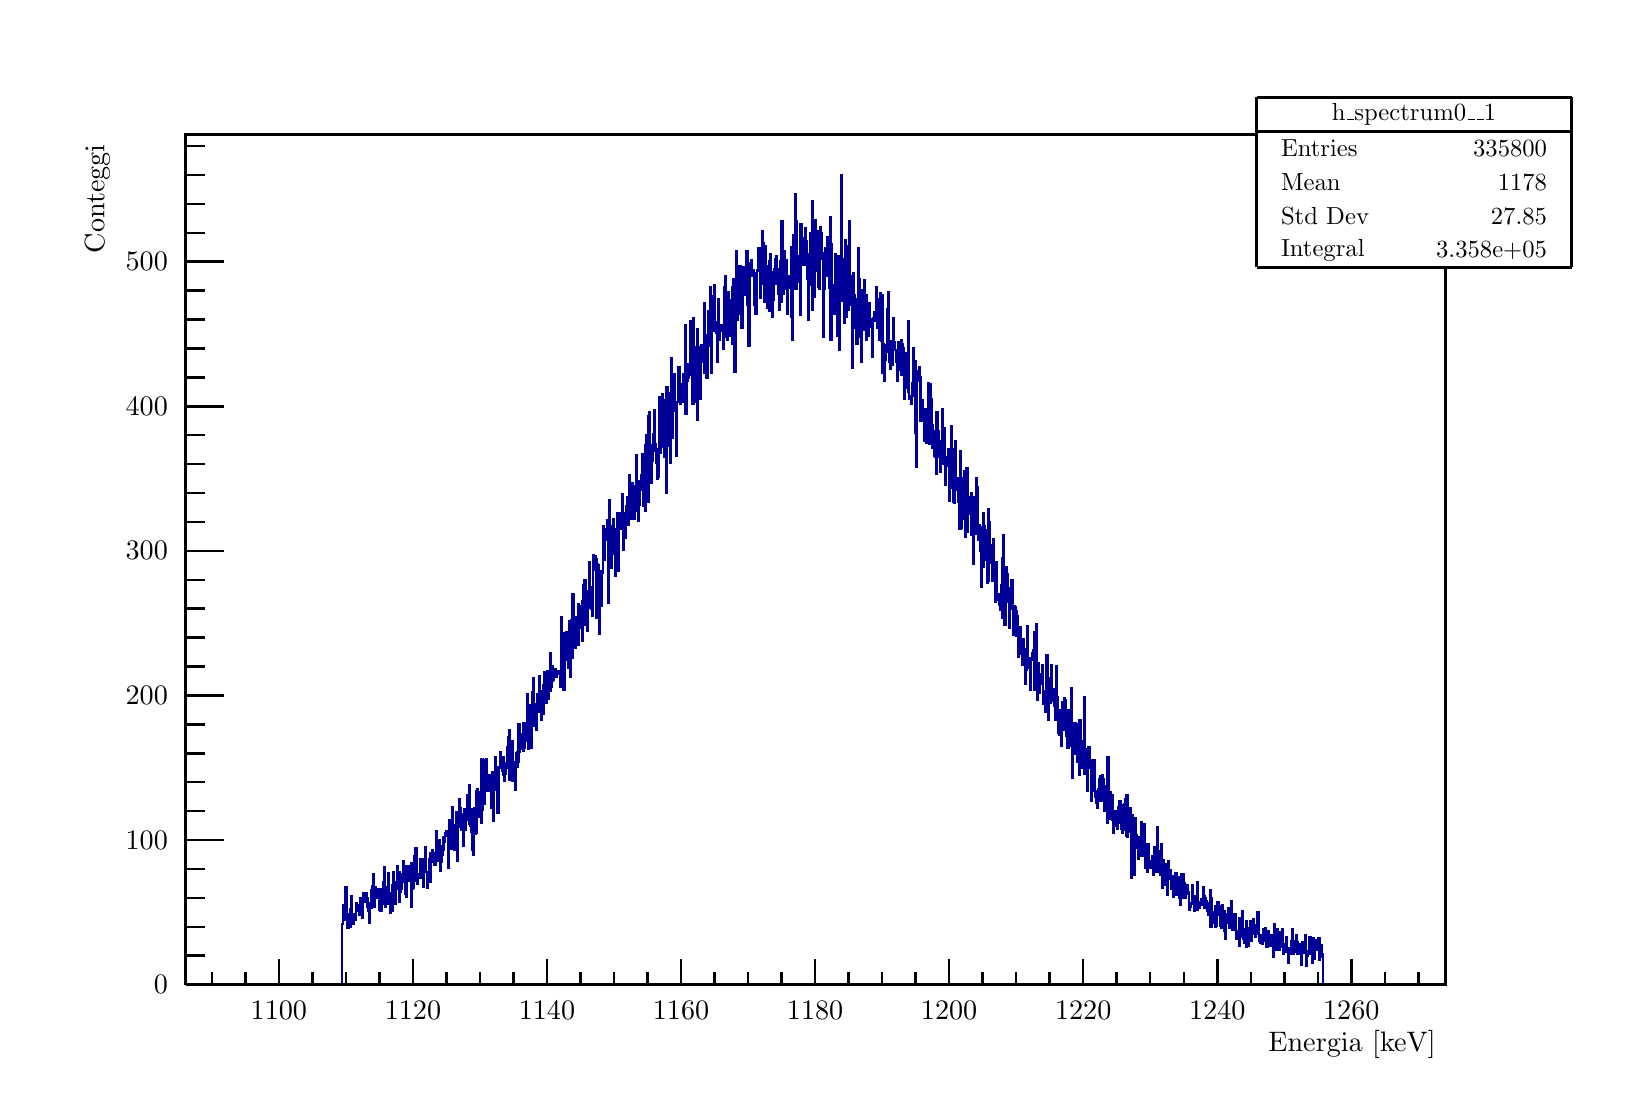
\begin{tikzpicture}
\pgfdeclareplotmark{cross} {
\pgfpathmoveto{\pgfpoint{-0.3\pgfplotmarksize}{\pgfplotmarksize}}
\pgfpathlineto{\pgfpoint{+0.3\pgfplotmarksize}{\pgfplotmarksize}}
\pgfpathlineto{\pgfpoint{+0.3\pgfplotmarksize}{0.3\pgfplotmarksize}}
\pgfpathlineto{\pgfpoint{+1\pgfplotmarksize}{0.3\pgfplotmarksize}}
\pgfpathlineto{\pgfpoint{+1\pgfplotmarksize}{-0.3\pgfplotmarksize}}
\pgfpathlineto{\pgfpoint{+0.3\pgfplotmarksize}{-0.3\pgfplotmarksize}}
\pgfpathlineto{\pgfpoint{+0.3\pgfplotmarksize}{-1.\pgfplotmarksize}}
\pgfpathlineto{\pgfpoint{-0.3\pgfplotmarksize}{-1.\pgfplotmarksize}}
\pgfpathlineto{\pgfpoint{-0.3\pgfplotmarksize}{-0.3\pgfplotmarksize}}
\pgfpathlineto{\pgfpoint{-1.\pgfplotmarksize}{-0.3\pgfplotmarksize}}
\pgfpathlineto{\pgfpoint{-1.\pgfplotmarksize}{0.3\pgfplotmarksize}}
\pgfpathlineto{\pgfpoint{-0.3\pgfplotmarksize}{0.3\pgfplotmarksize}}
\pgfpathclose
\pgfusepathqstroke
}
\pgfdeclareplotmark{cross*} {
\pgfpathmoveto{\pgfpoint{-0.3\pgfplotmarksize}{\pgfplotmarksize}}
\pgfpathlineto{\pgfpoint{+0.3\pgfplotmarksize}{\pgfplotmarksize}}
\pgfpathlineto{\pgfpoint{+0.3\pgfplotmarksize}{0.3\pgfplotmarksize}}
\pgfpathlineto{\pgfpoint{+1\pgfplotmarksize}{0.3\pgfplotmarksize}}
\pgfpathlineto{\pgfpoint{+1\pgfplotmarksize}{-0.3\pgfplotmarksize}}
\pgfpathlineto{\pgfpoint{+0.3\pgfplotmarksize}{-0.3\pgfplotmarksize}}
\pgfpathlineto{\pgfpoint{+0.3\pgfplotmarksize}{-1.\pgfplotmarksize}}
\pgfpathlineto{\pgfpoint{-0.3\pgfplotmarksize}{-1.\pgfplotmarksize}}
\pgfpathlineto{\pgfpoint{-0.3\pgfplotmarksize}{-0.3\pgfplotmarksize}}
\pgfpathlineto{\pgfpoint{-1.\pgfplotmarksize}{-0.3\pgfplotmarksize}}
\pgfpathlineto{\pgfpoint{-1.\pgfplotmarksize}{0.3\pgfplotmarksize}}
\pgfpathlineto{\pgfpoint{-0.3\pgfplotmarksize}{0.3\pgfplotmarksize}}
\pgfpathclose
\pgfusepathqfillstroke
}
\pgfdeclareplotmark{newstar} {
\pgfpathmoveto{\pgfqpoint{0pt}{\pgfplotmarksize}}
\pgfpathlineto{\pgfqpointpolar{44}{0.5\pgfplotmarksize}}
\pgfpathlineto{\pgfqpointpolar{18}{\pgfplotmarksize}}
\pgfpathlineto{\pgfqpointpolar{-20}{0.5\pgfplotmarksize}}
\pgfpathlineto{\pgfqpointpolar{-54}{\pgfplotmarksize}}
\pgfpathlineto{\pgfqpointpolar{-90}{0.5\pgfplotmarksize}}
\pgfpathlineto{\pgfqpointpolar{234}{\pgfplotmarksize}}
\pgfpathlineto{\pgfqpointpolar{198}{0.5\pgfplotmarksize}}
\pgfpathlineto{\pgfqpointpolar{162}{\pgfplotmarksize}}
\pgfpathlineto{\pgfqpointpolar{134}{0.5\pgfplotmarksize}}
\pgfpathclose
\pgfusepathqstroke
}
\pgfdeclareplotmark{newstar*} {
\pgfpathmoveto{\pgfqpoint{0pt}{\pgfplotmarksize}}
\pgfpathlineto{\pgfqpointpolar{44}{0.5\pgfplotmarksize}}
\pgfpathlineto{\pgfqpointpolar{18}{\pgfplotmarksize}}
\pgfpathlineto{\pgfqpointpolar{-20}{0.5\pgfplotmarksize}}
\pgfpathlineto{\pgfqpointpolar{-54}{\pgfplotmarksize}}
\pgfpathlineto{\pgfqpointpolar{-90}{0.5\pgfplotmarksize}}
\pgfpathlineto{\pgfqpointpolar{234}{\pgfplotmarksize}}
\pgfpathlineto{\pgfqpointpolar{198}{0.5\pgfplotmarksize}}
\pgfpathlineto{\pgfqpointpolar{162}{\pgfplotmarksize}}
\pgfpathlineto{\pgfqpointpolar{134}{0.5\pgfplotmarksize}}
\pgfpathclose
\pgfusepathqfillstroke
}
\definecolor{c}{rgb}{1,1,1};
\draw [color=c, fill=c] (0,0) rectangle (20,13.4957);
\draw [color=c, fill=c] (2,1.34957) rectangle (18,12.1461);
\definecolor{c}{rgb}{0,0,0};
\draw [c,line width=0.9] (2,1.34957) -- (2,12.1461) -- (18,12.1461) -- (18,1.34957) -- (2,1.34957);
\definecolor{c}{rgb}{1,1,1};
\draw [color=c, fill=c] (2,1.34957) rectangle (18,12.1461);
\definecolor{c}{rgb}{0,0,0};
\draw [c,line width=0.9] (2,1.34957) -- (2,12.1461) -- (18,12.1461) -- (18,1.34957) -- (2,1.34957);
\definecolor{c}{rgb}{0,0,0.6};
\draw [c,line width=0.9] (2,1.34957) -- (2.0089,1.34957) -- (2.0089,1.34957) -- (2.01781,1.34957) -- (2.01781,1.34957) -- (2.02671,1.34957) -- (2.02671,1.34957) -- (2.03561,1.34957) -- (2.03561,1.34957) -- (2.04452,1.34957) -- (2.04452,1.34957) --
 (2.05342,1.34957) -- (2.05342,1.34957) -- (2.06233,1.34957) -- (2.06233,1.34957) -- (2.07123,1.34957) -- (2.07123,1.34957) -- (2.08013,1.34957) -- (2.08013,1.34957) -- (2.08904,1.34957) -- (2.08904,1.34957) -- (2.09794,1.34957) -- (2.09794,1.34957)
 -- (2.10684,1.34957) -- (2.10684,1.34957) -- (2.11575,1.34957) -- (2.11575,1.34957) -- (2.12465,1.34957) -- (2.12465,1.34957) -- (2.13356,1.34957) -- (2.13356,1.34957) -- (2.14246,1.34957) -- (2.14246,1.34957) -- (2.15136,1.34957) --
 (2.15136,1.34957) -- (2.16027,1.34957) -- (2.16027,1.34957) -- (2.16917,1.34957) -- (2.16917,1.34957) -- (2.17807,1.34957) -- (2.17807,1.34957) -- (2.18698,1.34957) -- (2.18698,1.34957) -- (2.19588,1.34957) -- (2.19588,1.34957) -- (2.20479,1.34957)
 -- (2.20479,1.34957) -- (2.21369,1.34957) -- (2.21369,1.34957) -- (2.22259,1.34957) -- (2.22259,1.34957) -- (2.2315,1.34957) -- (2.2315,1.34957) -- (2.2404,1.34957) -- (2.2404,1.34957) -- (2.2493,1.34957) -- (2.2493,1.34957) -- (2.25821,1.34957) --
 (2.25821,1.34957) -- (2.26711,1.34957) -- (2.26711,1.34957) -- (2.27602,1.34957) -- (2.27602,1.34957) -- (2.28492,1.34957) -- (2.28492,1.34957) -- (2.29382,1.34957) -- (2.29382,1.34957) -- (2.30273,1.34957) -- (2.30273,1.34957) -- (2.31163,1.34957)
 -- (2.31163,1.34957) -- (2.32053,1.34957) -- (2.32053,1.34957) -- (2.32944,1.34957) -- (2.32944,1.34957) -- (2.33834,1.34957) -- (2.33834,1.34957) -- (2.34725,1.34957) -- (2.34725,1.34957) -- (2.35615,1.34957) -- (2.35615,1.34957) --
 (2.36505,1.34957) -- (2.36505,1.34957) -- (2.37396,1.34957) -- (2.37396,1.34957) -- (2.38286,1.34957) -- (2.38286,1.34957) -- (2.39176,1.34957) -- (2.39176,1.34957) -- (2.40067,1.34957) -- (2.40067,1.34957) -- (2.40957,1.34957) -- (2.40957,1.34957)
 -- (2.41848,1.34957) -- (2.41848,1.34957) -- (2.42738,1.34957) -- (2.42738,1.34957) -- (2.43628,1.34957) -- (2.43628,1.34957) -- (2.44519,1.34957) -- (2.44519,1.34957) -- (2.45409,1.34957) -- (2.45409,1.34957) -- (2.46299,1.34957) --
 (2.46299,1.34957) -- (2.4719,1.34957) -- (2.4719,1.34957) -- (2.4808,1.34957) -- (2.4808,1.34957) -- (2.48971,1.34957) -- (2.48971,1.34957) -- (2.49861,1.34957) -- (2.49861,1.34957) -- (2.50751,1.34957) -- (2.50751,1.34957) -- (2.51642,1.34957) --
 (2.51642,1.34957) -- (2.52532,1.34957) -- (2.52532,1.34957) -- (2.53422,1.34957) -- (2.53422,1.34957) -- (2.54313,1.34957) -- (2.54313,1.34957) -- (2.55203,1.34957) -- (2.55203,1.34957) -- (2.56094,1.34957) -- (2.56094,1.34957) -- (2.56984,1.34957)
 -- (2.56984,1.34957) -- (2.57874,1.34957) -- (2.57874,1.34957) -- (2.58765,1.34957) -- (2.58765,1.34957) -- (2.59655,1.34957) -- (2.59655,1.34957) -- (2.60545,1.34957) -- (2.60545,1.34957) -- (2.61436,1.34957) -- (2.61436,1.34957) --
 (2.62326,1.34957) -- (2.62326,1.34957) -- (2.63216,1.34957) -- (2.63216,1.34957) -- (2.64107,1.34957) -- (2.64107,1.34957) -- (2.64997,1.34957) -- (2.64997,1.34957) -- (2.65888,1.34957) -- (2.65888,1.34957) -- (2.66778,1.34957) -- (2.66778,1.34957)
 -- (2.67668,1.34957) -- (2.67668,1.34957) -- (2.68559,1.34957) -- (2.68559,1.34957) -- (2.69449,1.34957) -- (2.69449,1.34957) -- (2.70339,1.34957) -- (2.70339,1.34957) -- (2.7123,1.34957) -- (2.7123,1.34957) -- (2.7212,1.34957) -- (2.7212,1.34957)
 -- (2.73011,1.34957) -- (2.73011,1.34957) -- (2.73901,1.34957) -- (2.73901,1.34957) -- (2.74791,1.34957) -- (2.74791,1.34957) -- (2.75682,1.34957) -- (2.75682,1.34957) -- (2.76572,1.34957) -- (2.76572,1.34957) -- (2.77462,1.34957) --
 (2.77462,1.34957) -- (2.78353,1.34957) -- (2.78353,1.34957) -- (2.79243,1.34957) -- (2.79243,1.34957) -- (2.80134,1.34957) -- (2.80134,1.34957) -- (2.81024,1.34957) -- (2.81024,1.34957) -- (2.81914,1.34957) -- (2.81914,1.34957) -- (2.82805,1.34957)
 -- (2.82805,1.34957) -- (2.83695,1.34957) -- (2.83695,1.34957) -- (2.84585,1.34957) -- (2.84585,1.34957) -- (2.85476,1.34957) -- (2.85476,1.34957) -- (2.86366,1.34957) -- (2.86366,1.34957) -- (2.87257,1.34957) -- (2.87257,1.34957) --
 (2.88147,1.34957) -- (2.88147,1.34957) -- (2.89037,1.34957) -- (2.89037,1.34957) -- (2.89928,1.34957) -- (2.89928,1.34957) -- (2.90818,1.34957) -- (2.90818,1.34957) -- (2.91708,1.34957) -- (2.91708,1.34957) -- (2.92599,1.34957) -- (2.92599,1.34957)
 -- (2.93489,1.34957) -- (2.93489,1.34957) -- (2.9438,1.34957) -- (2.9438,1.34957) -- (2.9527,1.34957) -- (2.9527,1.34957) -- (2.9616,1.34957) -- (2.9616,1.34957) -- (2.97051,1.34957) -- (2.97051,1.34957) -- (2.97941,1.34957) -- (2.97941,1.34957) --
 (2.98831,1.34957) -- (2.98831,1.34957) -- (2.99722,1.34957) -- (2.99722,1.34957) -- (3.00612,1.34957) -- (3.00612,1.34957) -- (3.01503,1.34957) -- (3.01503,1.34957) -- (3.02393,1.34957) -- (3.02393,1.34957) -- (3.03283,1.34957) -- (3.03283,1.34957)
 -- (3.04174,1.34957) -- (3.04174,1.34957) -- (3.05064,1.34957) -- (3.05064,1.34957) -- (3.05954,1.34957) -- (3.05954,1.34957) -- (3.06845,1.34957) -- (3.06845,1.34957) -- (3.07735,1.34957) -- (3.07735,1.34957) -- (3.08626,1.34957) --
 (3.08626,1.34957) -- (3.09516,1.34957) -- (3.09516,1.34957) -- (3.10406,1.34957) -- (3.10406,1.34957) -- (3.11297,1.34957) -- (3.11297,1.34957) -- (3.12187,1.34957) -- (3.12187,1.34957) -- (3.13077,1.34957) -- (3.13077,1.34957) -- (3.13968,1.34957)
 -- (3.13968,1.34957) -- (3.14858,1.34957) -- (3.14858,1.34957) -- (3.15748,1.34957) -- (3.15748,1.34957) -- (3.16639,1.34957) -- (3.16639,1.34957) -- (3.17529,1.34957) -- (3.17529,1.34957) -- (3.1842,1.34957) -- (3.1842,1.34957) -- (3.1931,1.34957)
 -- (3.1931,1.34957) -- (3.202,1.34957) -- (3.202,1.34957) -- (3.21091,1.34957) -- (3.21091,1.34957) -- (3.21981,1.34957) -- (3.21981,1.34957) -- (3.22871,1.34957) -- (3.22871,1.34957) -- (3.23762,1.34957) -- (3.23762,1.34957) -- (3.24652,1.34957) --
 (3.24652,1.34957) -- (3.25543,1.34957) -- (3.25543,1.34957) -- (3.26433,1.34957) -- (3.26433,1.34957) -- (3.27323,1.34957) -- (3.27323,1.34957) -- (3.28214,1.34957) -- (3.28214,1.34957) -- (3.29104,1.34957) -- (3.29104,1.34957) -- (3.29994,1.34957)
 -- (3.29994,1.34957) -- (3.30885,1.34957) -- (3.30885,1.34957) -- (3.31775,1.34957) -- (3.31775,1.34957) -- (3.32666,1.34957) -- (3.32666,1.34957) -- (3.33556,1.34957) -- (3.33556,1.34957) -- (3.34446,1.34957) -- (3.34446,1.34957) --
 (3.35337,1.34957) -- (3.35337,1.34957) -- (3.36227,1.34957) -- (3.36227,1.34957) -- (3.37117,1.34957) -- (3.37117,1.34957) -- (3.38008,1.34957) -- (3.38008,1.34957) -- (3.38898,1.34957) -- (3.38898,1.34957) -- (3.39789,1.34957) -- (3.39789,1.34957)
 -- (3.40679,1.34957) -- (3.40679,1.34957) -- (3.41569,1.34957) -- (3.41569,1.34957) -- (3.4246,1.34957) -- (3.4246,1.34957) -- (3.4335,1.34957) -- (3.4335,1.34957) -- (3.4424,1.34957) -- (3.4424,1.34957) -- (3.45131,1.34957) -- (3.45131,1.34957) --
 (3.46021,1.34957) -- (3.46021,1.34957) -- (3.46912,1.34957) -- (3.46912,1.34957) -- (3.47802,1.34957) -- (3.47802,1.34957) -- (3.48692,1.34957) -- (3.48692,1.34957) -- (3.49583,1.34957) -- (3.49583,1.34957) -- (3.50473,1.34957) -- (3.50473,1.34957)
 -- (3.51363,1.34957) -- (3.51363,1.34957) -- (3.52254,1.34957) -- (3.52254,1.34957) -- (3.53144,1.34957) -- (3.53144,1.34957) -- (3.54035,1.34957) -- (3.54035,1.34957) -- (3.54925,1.34957) -- (3.54925,1.34957) -- (3.55815,1.34957) --
 (3.55815,1.34957) -- (3.56706,1.34957) -- (3.56706,1.34957) -- (3.57596,1.34957) -- (3.57596,1.34957) -- (3.58486,1.34957) -- (3.58486,1.34957) -- (3.59377,1.34957) -- (3.59377,1.34957) -- (3.60267,1.34957) -- (3.60267,1.34957) -- (3.61157,1.34957)
 -- (3.61157,1.34957) -- (3.62048,1.34957) -- (3.62048,1.34957) -- (3.62938,1.34957) -- (3.62938,1.34957) -- (3.63829,1.34957) -- (3.63829,1.34957) -- (3.64719,1.34957) -- (3.64719,1.34957) -- (3.65609,1.34957) -- (3.65609,1.34957) -- (3.665,1.34957)
 -- (3.665,1.34957) -- (3.6739,1.34957) -- (3.6739,1.34957) -- (3.6828,1.34957) -- (3.6828,1.34957) -- (3.69171,1.34957) -- (3.69171,1.34957) -- (3.70061,1.34957) -- (3.70061,1.34957) -- (3.70952,1.34957) -- (3.70952,1.34957) -- (3.71842,1.34957) --
 (3.71842,1.34957) -- (3.72732,1.34957) -- (3.72732,1.34957) -- (3.73623,1.34957) -- (3.73623,1.34957) -- (3.74513,1.34957) -- (3.74513,1.34957) -- (3.75403,1.34957) -- (3.75403,1.34957) -- (3.76294,1.34957) -- (3.76294,1.34957) -- (3.77184,1.34957)
 -- (3.77184,1.34957) -- (3.78075,1.34957) -- (3.78075,1.34957) -- (3.78965,1.34957) -- (3.78965,1.34957) -- (3.79855,1.34957) -- (3.79855,1.34957) -- (3.80746,1.34957) -- (3.80746,1.34957) -- (3.81636,1.34957) -- (3.81636,1.34957) --
 (3.82526,1.34957) -- (3.82526,1.34957) -- (3.83417,1.34957) -- (3.83417,1.34957) -- (3.84307,1.34957) -- (3.84307,1.34957) -- (3.85198,1.34957) -- (3.85198,1.34957) -- (3.86088,1.34957) -- (3.86088,1.34957) -- (3.86978,1.34957) -- (3.86978,1.34957)
 -- (3.87869,1.34957) -- (3.87869,1.34957) -- (3.88759,1.34957) -- (3.88759,1.34957) -- (3.89649,1.34957) -- (3.89649,1.34957) -- (3.9054,1.34957) -- (3.9054,1.34957) -- (3.9143,1.34957) -- (3.9143,1.34957) -- (3.92321,1.34957) -- (3.92321,1.34957)
 -- (3.93211,1.34957) -- (3.93211,1.34957) -- (3.94101,1.34957) -- (3.94101,1.34957) -- (3.94992,1.34957) -- (3.94992,1.34957) -- (3.95882,1.34957) -- (3.95882,1.34957) -- (3.96772,1.34957) -- (3.96772,1.34957) -- (3.97663,1.34957) --
 (3.97663,1.34957) -- (3.98553,1.34957) -- (3.98553,2.12075) -- (3.99444,2.12075) -- (3.99444,2.32273) -- (4.00334,2.32273) -- (4.00334,2.35945) -- (4.01224,2.35945) -- (4.01224,2.17584) -- (4.02115,2.17584) -- (4.02115,2.17584) -- (4.03005,2.17584)
 -- (4.03005,2.57979) -- (4.03895,2.57979) -- (4.03895,2.23092) -- (4.04786,2.23092) -- (4.04786,2.24928) -- (4.05676,2.24928) -- (4.05676,2.06567) -- (4.06567,2.06567) -- (4.06567,2.08403) -- (4.07457,2.08403) -- (4.07457,2.23092) --
 (4.08347,2.23092) -- (4.08347,2.08403) -- (4.09238,2.08403) -- (4.09238,2.30437) -- (4.10128,2.30437) -- (4.10128,2.46962) -- (4.11018,2.46962) -- (4.11018,2.24928) -- (4.11909,2.24928) -- (4.11909,2.12075) -- (4.12799,2.12075) -- (4.12799,2.1942)
 -- (4.13689,2.1942) -- (4.13689,2.1942) -- (4.1458,2.1942) -- (4.1458,2.17584) -- (4.1547,2.17584) -- (4.1547,2.24928) -- (4.16361,2.24928) -- (4.16361,2.37781) -- (4.17251,2.37781) -- (4.17251,2.32273) -- (4.18141,2.32273) -- (4.18141,2.28601) --
 (4.19032,2.28601) -- (4.19032,2.35945) -- (4.19922,2.35945) -- (4.19922,2.23092) -- (4.20812,2.23092) -- (4.20812,2.23092) -- (4.21703,2.23092) -- (4.21703,2.45126) -- (4.22593,2.45126) -- (4.22593,2.4329) -- (4.23484,2.4329) -- (4.23484,2.30437) --
 (4.24374,2.30437) -- (4.24374,2.1942) -- (4.25264,2.1942) -- (4.25264,2.50634) -- (4.26155,2.50634) -- (4.26155,2.4329) -- (4.27045,2.4329) -- (4.27045,2.39618) -- (4.27935,2.39618) -- (4.27935,2.50634) -- (4.28826,2.50634) -- (4.28826,2.50634) --
 (4.29716,2.50634) -- (4.29716,2.45126) -- (4.30607,2.45126) -- (4.30607,2.34109) -- (4.31497,2.34109) -- (4.31497,2.35945) -- (4.32387,2.35945) -- (4.32387,2.28601) -- (4.33278,2.28601) -- (4.33278,2.13911) -- (4.34168,2.13911) -- (4.34168,2.37781)
 -- (4.35058,2.37781) -- (4.35058,2.32273) -- (4.35949,2.32273) -- (4.35949,2.54307) -- (4.36839,2.54307) -- (4.36839,2.59815) -- (4.3773,2.59815) -- (4.3773,2.74504) -- (4.3862,2.74504) -- (4.3862,2.34109) -- (4.3951,2.34109) -- (4.3951,2.37781) --
 (4.40401,2.37781) -- (4.40401,2.57979) -- (4.41291,2.57979) -- (4.41291,2.48798) -- (4.42181,2.48798) -- (4.42181,2.45126) -- (4.43072,2.45126) -- (4.43072,2.52471) -- (4.43962,2.52471) -- (4.43962,2.54307) -- (4.44853,2.54307) -- (4.44853,2.56143)
 -- (4.45743,2.56143) -- (4.45743,2.30437) -- (4.46633,2.30437) -- (4.46633,2.54307) -- (4.47524,2.54307) -- (4.47524,2.28601) -- (4.48414,2.28601) -- (4.48414,2.56143) -- (4.49304,2.56143) -- (4.49304,2.56143) -- (4.50195,2.56143) --
 (4.50195,2.37781) -- (4.51085,2.37781) -- (4.51085,2.65324) -- (4.51976,2.65324) -- (4.51976,2.83685) -- (4.52866,2.83685) -- (4.52866,2.34109) -- (4.53756,2.34109) -- (4.53756,2.54307) -- (4.54647,2.54307) -- (4.54647,2.57979) -- (4.55537,2.57979)
 -- (4.55537,2.37781) -- (4.56427,2.37781) -- (4.56427,2.50634) -- (4.57318,2.50634) -- (4.57318,2.76341) -- (4.58208,2.76341) -- (4.58208,2.50634) -- (4.59098,2.50634) -- (4.59098,2.45126) -- (4.59989,2.45126) -- (4.59989,2.26765) --
 (4.60879,2.26765) -- (4.60879,2.48798) -- (4.6177,2.48798) -- (4.6177,2.61651) -- (4.6266,2.61651) -- (4.6266,2.28601) -- (4.6355,2.28601) -- (4.6355,2.78177) -- (4.64441,2.78177) -- (4.64441,2.59815) -- (4.65331,2.59815) -- (4.65331,2.63488) --
 (4.66221,2.63488) -- (4.66221,2.37781) -- (4.67112,2.37781) -- (4.67112,2.56143) -- (4.68002,2.56143) -- (4.68002,2.65324) -- (4.68893,2.65324) -- (4.68893,2.85521) -- (4.69783,2.85521) -- (4.69783,2.68996) -- (4.70673,2.68996) -- (4.70673,2.78177)
 -- (4.71564,2.78177) -- (4.71564,2.39618) -- (4.72454,2.39618) -- (4.72454,2.52471) -- (4.73344,2.52471) -- (4.73344,2.56143) -- (4.74235,2.56143) -- (4.74235,2.74504) -- (4.75125,2.74504) -- (4.75125,2.65324) -- (4.76016,2.65324) --
 (4.76016,2.9103) -- (4.76906,2.9103) -- (4.76906,2.80013) -- (4.77796,2.80013) -- (4.77796,2.6716) -- (4.78687,2.6716) -- (4.78687,2.50634) -- (4.79577,2.50634) -- (4.79577,2.46962) -- (4.80467,2.46962) -- (4.80467,2.85521) -- (4.81358,2.85521) --
 (4.81358,2.72668) -- (4.82248,2.72668) -- (4.82248,2.6716) -- (4.83139,2.6716) -- (4.83139,2.68996) -- (4.84029,2.68996) -- (4.84029,2.85521) -- (4.84919,2.85521) -- (4.84919,2.68996) -- (4.8581,2.68996) -- (4.8581,2.34109) -- (4.867,2.34109) --
 (4.867,2.89194) -- (4.8759,2.89194) -- (4.8759,2.56143) -- (4.88481,2.56143) -- (4.88481,2.57979) -- (4.89371,2.57979) -- (4.89371,2.6716) -- (4.90262,2.6716) -- (4.90262,2.98374) -- (4.91152,2.98374) -- (4.91152,2.74504) -- (4.92042,2.74504) --
 (4.92042,3.07555) -- (4.92933,3.07555) -- (4.92933,2.92866) -- (4.93823,2.92866) -- (4.93823,2.63488) -- (4.94713,2.63488) -- (4.94713,2.72668) -- (4.95604,2.72668) -- (4.95604,2.74504) -- (4.96494,2.74504) -- (4.96494,2.74504) -- (4.97385,2.74504)
 -- (4.97385,2.70832) -- (4.98275,2.70832) -- (4.98275,2.94702) -- (4.99165,2.94702) -- (4.99165,2.83685) -- (5.00056,2.83685) -- (5.00056,2.94702) -- (5.00946,2.94702) -- (5.00946,2.94702) -- (5.01836,2.94702) -- (5.01836,2.59815) --
 (5.02727,2.59815) -- (5.02727,2.85521) -- (5.03617,2.85521) -- (5.03617,2.85521) -- (5.04508,2.85521) -- (5.04508,3.09391) -- (5.05398,3.09391) -- (5.05398,2.78177) -- (5.06288,2.78177) -- (5.06288,2.57979) -- (5.07179,2.57979) -- (5.07179,2.70832)
 -- (5.08069,2.70832) -- (5.08069,2.70832) -- (5.08959,2.70832) -- (5.08959,2.94702) -- (5.0985,2.94702) -- (5.0985,2.65324) -- (5.1074,2.65324) -- (5.1074,3.02047) -- (5.1163,3.02047) -- (5.1163,2.96538) -- (5.12521,2.96538) -- (5.12521,2.9103) --
 (5.13411,2.9103) -- (5.13411,3.05719) -- (5.14302,3.05719) -- (5.14302,2.96538) -- (5.15192,2.96538) -- (5.15192,3.02047) -- (5.16082,3.02047) -- (5.16082,2.87357) -- (5.16973,2.87357) -- (5.16973,3.02047) -- (5.17863,3.02047) -- (5.17863,3.29589)
 -- (5.18753,3.29589) -- (5.18753,2.98374) -- (5.19644,2.98374) -- (5.19644,2.92866) -- (5.20534,2.92866) -- (5.20534,2.98374) -- (5.21425,2.98374) -- (5.21425,3.18572) -- (5.22315,3.18572) -- (5.22315,3.18572) -- (5.23205,3.18572) --
 (5.23205,2.80013) -- (5.24096,2.80013) -- (5.24096,2.9103) -- (5.24986,2.9103) -- (5.24986,3.00211) -- (5.25876,3.00211) -- (5.25876,3.11227) -- (5.26767,3.11227) -- (5.26767,3.05719) -- (5.27657,3.05719) -- (5.27657,3.22244) -- (5.28548,3.22244) --
 (5.28548,3.16736) -- (5.29438,3.16736) -- (5.29438,3.27753) -- (5.30328,3.27753) -- (5.30328,3.2408) -- (5.31219,3.2408) -- (5.31219,3.29589) -- (5.32109,3.29589) -- (5.32109,3.2408) -- (5.32999,3.2408) -- (5.32999,2.83685) -- (5.3389,2.83685) --
 (5.3389,3.2408) -- (5.3478,3.2408) -- (5.3478,3.44278) -- (5.35671,3.44278) -- (5.35671,3.07555) -- (5.36561,3.07555) -- (5.36561,3.11227) -- (5.37451,3.11227) -- (5.37451,3.27753) -- (5.38342,3.27753) -- (5.38342,3.60803) -- (5.39232,3.60803) --
 (5.39232,3.27753) -- (5.40122,3.27753) -- (5.40122,3.07555) -- (5.41013,3.07555) -- (5.41013,3.05719) -- (5.41903,3.05719) -- (5.41903,3.36934) -- (5.42794,3.36934) -- (5.42794,3.07555) -- (5.43684,3.07555) -- (5.43684,3.53459) -- (5.44574,3.53459)
 -- (5.44574,2.92866) -- (5.45465,2.92866) -- (5.45465,3.51623) -- (5.46355,3.51623) -- (5.46355,3.44278) -- (5.47245,3.44278) -- (5.47245,3.69984) -- (5.48136,3.69984) -- (5.48136,3.58967) -- (5.49026,3.58967) -- (5.49026,3.35097) --
 (5.49917,3.35097) -- (5.49917,3.31425) -- (5.50807,3.31425) -- (5.50807,3.33261) -- (5.51697,3.33261) -- (5.51697,3.51623) -- (5.52588,3.51623) -- (5.52588,3.11227) -- (5.53478,3.11227) -- (5.53478,3.57131) -- (5.54368,3.57131) -- (5.54368,3.44278)
 -- (5.55259,3.44278) -- (5.55259,3.31425) -- (5.56149,3.31425) -- (5.56149,3.44278) -- (5.57039,3.44278) -- (5.57039,3.75493) -- (5.5793,3.75493) -- (5.5793,3.51623) -- (5.5882,3.51623) -- (5.5882,3.4795) -- (5.59711,3.4795) -- (5.59711,3.88346) --
 (5.60601,3.88346) -- (5.60601,3.3877) -- (5.61491,3.3877) -- (5.61491,3.36934) -- (5.62382,3.36934) -- (5.62382,3.29589) -- (5.63272,3.29589) -- (5.63272,3.57131) -- (5.64162,3.57131) -- (5.64162,3.05719) -- (5.65053,3.05719) -- (5.65053,3.00211) --
 (5.65943,3.00211) -- (5.65943,3.58967) -- (5.66834,3.58967) -- (5.66834,3.57131) -- (5.67724,3.57131) -- (5.67724,3.25917) -- (5.68614,3.25917) -- (5.68614,3.27753) -- (5.69505,3.27753) -- (5.69505,3.81001) -- (5.70395,3.81001) -- (5.70395,3.82837)
 -- (5.71285,3.82837) -- (5.71285,3.79165) -- (5.72176,3.79165) -- (5.72176,3.53459) -- (5.73066,3.53459) -- (5.73066,3.4795) -- (5.73957,3.4795) -- (5.73957,3.73657) -- (5.74847,3.73657) -- (5.74847,3.40606) -- (5.75737,3.40606) -- (5.75737,4.21396)
 -- (5.76628,4.21396) -- (5.76628,3.57131) -- (5.77518,3.57131) -- (5.77518,4.15888) -- (5.78408,4.15888) -- (5.78408,4.1956) -- (5.79299,4.1956) -- (5.79299,3.64476) -- (5.80189,3.64476) -- (5.80189,3.84673) -- (5.8108,3.84673) -- (5.8108,4.21396)
 -- (5.8197,4.21396) -- (5.8197,3.82837) -- (5.8286,3.82837) -- (5.8286,3.81001) -- (5.83751,3.81001) -- (5.83751,3.9569) -- (5.84641,3.9569) -- (5.84641,4.01199) -- (5.85531,4.01199) -- (5.85531,3.82837) -- (5.86422,3.82837) -- (5.86422,3.92018) --
 (5.87312,3.92018) -- (5.87312,3.81001) -- (5.88203,3.81001) -- (5.88203,3.58967) -- (5.89093,3.58967) -- (5.89093,4.04871) -- (5.89983,4.04871) -- (5.89983,3.42442) -- (5.90874,3.42442) -- (5.90874,3.55295) -- (5.91764,3.55295) -- (5.91764,3.82837)
 -- (5.92654,3.82837) -- (5.92654,4.23233) -- (5.93545,4.23233) -- (5.93545,3.99363) -- (5.94435,3.99363) -- (5.94435,4.1038) -- (5.95326,4.1038) -- (5.95326,3.81001) -- (5.96216,3.81001) -- (5.96216,3.53459) -- (5.97106,3.53459) -- (5.97106,3.73657)
 -- (5.97997,3.73657) -- (5.97997,4.1038) -- (5.98887,4.1038) -- (5.98887,4.30577) -- (5.99777,4.30577) -- (5.99777,4.1956) -- (6.00668,4.1956) -- (6.00668,4.21396) -- (6.01558,4.21396) -- (6.01558,4.06707) -- (6.02449,4.06707) -- (6.02449,4.23233)
 -- (6.03339,4.23233) -- (6.03339,4.01199) -- (6.04229,4.01199) -- (6.04229,3.93854) -- (6.0512,3.93854) -- (6.0512,4.06707) -- (6.0601,4.06707) -- (6.0601,4.03035) -- (6.069,4.03035) -- (6.069,4.15888) -- (6.07791,4.15888) -- (6.07791,4.36086) --
 (6.08681,4.36086) -- (6.08681,4.1038) -- (6.09572,4.1038) -- (6.09572,4.48939) -- (6.10462,4.48939) -- (6.10462,4.58119) -- (6.11352,4.58119) -- (6.11352,3.9569) -- (6.12243,3.9569) -- (6.12243,4.26905) -- (6.13133,4.26905) -- (6.13133,4.06707) --
 (6.14023,4.06707) -- (6.14023,4.4343) -- (6.14914,4.4343) -- (6.14914,3.93854) -- (6.15804,3.93854) -- (6.15804,4.14052) -- (6.16694,4.14052) -- (6.16694,4.17724) -- (6.17585,4.17724) -- (6.17585,3.9569) -- (6.18475,3.9569) -- (6.18475,3.82837) --
 (6.19366,3.82837) -- (6.19366,4.28741) -- (6.20256,4.28741) -- (6.20256,4.12216) -- (6.21146,4.12216) -- (6.21146,4.30577) -- (6.22037,4.30577) -- (6.22037,4.17724) -- (6.22927,4.17724) -- (6.22927,4.65464) -- (6.23817,4.65464) -- (6.23817,4.30577)
 -- (6.24708,4.30577) -- (6.24708,4.45266) -- (6.25598,4.45266) -- (6.25598,4.34249) -- (6.26489,4.34249) -- (6.26489,4.52611) -- (6.27379,4.52611) -- (6.27379,4.37922) -- (6.28269,4.37922) -- (6.28269,4.32413) -- (6.2916,4.32413) -- (6.2916,4.673)
 -- (6.3005,4.673) -- (6.3005,4.36086) -- (6.3094,4.36086) -- (6.3094,4.52611) -- (6.31831,4.52611) -- (6.31831,4.54447) -- (6.32721,4.54447) -- (6.32721,4.45266) -- (6.33612,4.45266) -- (6.33612,5.04023) -- (6.34502,5.04023) -- (6.34502,4.34249) --
 (6.35392,4.34249) -- (6.35392,4.81989) -- (6.36283,4.81989) -- (6.36283,4.69136) -- (6.37173,4.69136) -- (6.37173,4.65464) -- (6.38063,4.65464) -- (6.38063,4.89334) -- (6.38954,4.89334) -- (6.38954,4.36086) -- (6.39844,4.36086) -- (6.39844,5.05859)
 -- (6.40735,5.05859) -- (6.40735,5.24221) -- (6.41625,5.24221) -- (6.41625,4.83825) -- (6.42515,4.83825) -- (6.42515,4.63628) -- (6.43406,4.63628) -- (6.43406,4.85662) -- (6.44296,4.85662) -- (6.44296,4.9117) -- (6.45186,4.9117) -- (6.45186,4.58119)
 -- (6.46077,4.58119) -- (6.46077,5.04023) -- (6.46967,5.04023) -- (6.46967,5.04023) -- (6.47858,5.04023) -- (6.47858,4.81989) -- (6.48748,4.81989) -- (6.48748,5.26057) -- (6.49638,5.26057) -- (6.49638,4.94842) -- (6.50529,4.94842) --
 (6.50529,5.02187) -- (6.51419,5.02187) -- (6.51419,4.70972) -- (6.52309,4.70972) -- (6.52309,5.07695) -- (6.532,5.07695) -- (6.532,4.78317) -- (6.5409,4.78317) -- (6.5409,5.1504) -- (6.54981,5.1504) -- (6.54981,5.31565) -- (6.55871,5.31565) --
 (6.55871,4.98515) -- (6.56761,4.98515) -- (6.56761,5.24221) -- (6.57652,5.24221) -- (6.57652,4.93006) -- (6.58542,4.93006) -- (6.58542,5.33402) -- (6.59432,5.33402) -- (6.59432,5.27893) -- (6.60323,5.27893) -- (6.60323,4.98515) -- (6.61213,4.98515)
 -- (6.61213,5.18712) -- (6.62104,5.18712) -- (6.62104,5.07695) -- (6.62994,5.07695) -- (6.62994,5.55435) -- (6.63884,5.55435) -- (6.63884,5.13204) -- (6.64775,5.13204) -- (6.64775,5.3891) -- (6.65665,5.3891) -- (6.65665,5.20548) -- (6.66555,5.20548)
 -- (6.66555,5.22385) -- (6.67446,5.22385) -- (6.67446,5.35238) -- (6.68336,5.35238) -- (6.68336,5.31565) -- (6.69227,5.31565) -- (6.69227,5.35238) -- (6.70117,5.35238) -- (6.70117,5.26057) -- (6.71007,5.26057) -- (6.71007,5.31565) --
 (6.71898,5.31565) -- (6.71898,5.29729) -- (6.72788,5.29729) -- (6.72788,5.33402) -- (6.73678,5.33402) -- (6.73678,5.29729) -- (6.74569,5.29729) -- (6.74569,5.31565) -- (6.75459,5.31565) -- (6.75459,5.13204) -- (6.76349,5.13204) -- (6.76349,6.01339)
 -- (6.7724,6.01339) -- (6.7724,5.48091) -- (6.7813,5.48091) -- (6.7813,5.31565) -- (6.79021,5.31565) -- (6.79021,5.75633) -- (6.79911,5.75633) -- (6.79911,5.09532) -- (6.80801,5.09532) -- (6.80801,5.81141) -- (6.81692,5.81141) -- (6.81692,5.64616)
 -- (6.82582,5.64616) -- (6.82582,5.48091) -- (6.83472,5.48091) -- (6.83472,5.82978) -- (6.84363,5.82978) -- (6.84363,5.73797) -- (6.85253,5.73797) -- (6.85253,5.37074) -- (6.86144,5.37074) -- (6.86144,5.40746) -- (6.87034,5.40746) --
 (6.87034,5.95831) -- (6.87924,5.95831) -- (6.87924,5.26057) -- (6.88815,5.26057) -- (6.88815,5.82978) -- (6.89705,5.82978) -- (6.89705,5.97667) -- (6.90595,5.97667) -- (6.90595,5.49927) -- (6.91486,5.49927) -- (6.91486,6.30718) -- (6.92376,6.30718)
 -- (6.92376,5.68288) -- (6.93267,5.68288) -- (6.93267,5.75633) -- (6.94157,5.75633) -- (6.94157,5.6278) -- (6.95047,5.6278) -- (6.95047,5.97667) -- (6.95938,5.97667) -- (6.95938,6.01339) -- (6.96828,6.01339) -- (6.96828,5.90322) -- (6.97718,5.90322)
 -- (6.97718,5.66452) -- (6.98609,5.66452) -- (6.98609,6.17864) -- (6.99499,6.17864) -- (6.99499,5.88486) -- (7.0039,5.88486) -- (7.0039,5.88486) -- (7.0128,5.88486) -- (7.0128,6.16028) -- (7.0217,6.16028) -- (7.0217,6.16028) -- (7.03061,6.16028) --
 (7.03061,5.71961) -- (7.03951,5.71961) -- (7.03951,6.21537) -- (7.04841,6.21537) -- (7.04841,6.41734) -- (7.05732,6.41734) -- (7.05732,5.92158) -- (7.06622,5.92158) -- (7.06622,6.49079) -- (7.07513,6.49079) -- (7.07513,5.95831) -- (7.08403,5.95831)
 -- (7.08403,6.03175) -- (7.09293,6.03175) -- (7.09293,6.3439) -- (7.10184,6.3439) -- (7.10184,5.84814) -- (7.11074,5.84814) -- (7.11074,6.14192) -- (7.11964,6.14192) -- (7.11964,6.71113) -- (7.12855,6.71113) -- (7.12855,6.36226) -- (7.13745,6.36226)
 -- (7.13745,6.39898) -- (7.14636,6.39898) -- (7.14636,6.12356) -- (7.15526,6.12356) -- (7.15526,6.32554) -- (7.16416,6.32554) -- (7.16416,6.03175) -- (7.17307,6.03175) -- (7.17307,6.80294) -- (7.18197,6.80294) -- (7.18197,6.61932) --
 (7.19087,6.61932) -- (7.19087,6.63768) -- (7.19978,6.63768) -- (7.19978,6.78457) -- (7.20868,6.78457) -- (7.20868,6.01339) -- (7.21759,6.01339) -- (7.21759,6.74785) -- (7.22649,6.74785) -- (7.22649,6.69277) -- (7.23539,6.69277) -- (7.23539,6.67441)
 -- (7.2443,6.67441) -- (7.2443,6.60096) -- (7.2532,6.60096) -- (7.2532,5.81141) -- (7.2621,5.81141) -- (7.2621,6.16028) -- (7.27101,6.16028) -- (7.27101,6.16028) -- (7.27991,6.16028) -- (7.27991,6.60096) -- (7.28881,6.60096) -- (7.28881,6.5826) --
 (7.29772,6.5826) -- (7.29772,7.17017) -- (7.30662,7.17017) -- (7.30662,6.74785) -- (7.31553,6.74785) -- (7.31553,6.78457) -- (7.32443,6.78457) -- (7.32443,7.04164) -- (7.33333,7.04164) -- (7.33333,7.00491) -- (7.34224,7.00491) -- (7.34224,7.13344)
 -- (7.35114,7.13344) -- (7.35114,7.24361) -- (7.36004,7.24361) -- (7.36004,6.19701) -- (7.36895,6.19701) -- (7.36895,6.93147) -- (7.37785,6.93147) -- (7.37785,7.50067) -- (7.38676,7.50067) -- (7.38676,6.87638) -- (7.39566,6.87638) --
 (7.39566,7.09672) -- (7.40456,7.09672) -- (7.40456,6.63768) -- (7.41347,6.63768) -- (7.41347,7.17017) -- (7.42237,7.17017) -- (7.42237,6.8213) -- (7.43127,6.8213) -- (7.43127,7.26197) -- (7.44018,7.26197) -- (7.44018,7.13344) -- (7.44908,7.13344) --
 (7.44908,6.54587) -- (7.45799,6.54587) -- (7.45799,6.9131) -- (7.46689,6.9131) -- (7.46689,6.69277) -- (7.47579,6.69277) -- (7.47579,7.33542) -- (7.4847,7.33542) -- (7.4847,6.60096) -- (7.4936,6.60096) -- (7.4936,7.09672) -- (7.5025,7.09672) --
 (7.5025,7.13344) -- (7.51141,7.13344) -- (7.51141,7.1518) -- (7.52031,7.1518) -- (7.52031,7.33542) -- (7.52922,7.33542) -- (7.52922,7.2987) -- (7.53812,7.2987) -- (7.53812,7.57412) -- (7.54702,7.57412) -- (7.54702,7.13344) -- (7.55593,7.13344) --
 (7.55593,6.87638) -- (7.56483,6.87638) -- (7.56483,7.06) -- (7.57373,7.06) -- (7.57373,7.33542) -- (7.58264,7.33542) -- (7.58264,7.02327) -- (7.59154,7.02327) -- (7.59154,7.42723) -- (7.60045,7.42723) -- (7.60045,7.37214) -- (7.60935,7.37214) --
 (7.60935,7.5374) -- (7.61825,7.5374) -- (7.61825,7.18853) -- (7.62716,7.18853) -- (7.62716,7.75773) -- (7.63606,7.75773) -- (7.63606,7.81282) -- (7.64496,7.81282) -- (7.64496,7.2987) -- (7.65387,7.2987) -- (7.65387,7.26197) -- (7.66277,7.26197) --
 (7.66277,7.72101) -- (7.67168,7.72101) -- (7.67168,7.70265) -- (7.68058,7.70265) -- (7.68058,7.33542) -- (7.68948,7.33542) -- (7.68948,7.33542) -- (7.69839,7.33542) -- (7.69839,7.26197) -- (7.70729,7.26197) -- (7.70729,7.68429) -- (7.71619,7.68429)
 -- (7.71619,8.06988) -- (7.7251,8.06988) -- (7.7251,7.68429) -- (7.734,7.68429) -- (7.734,7.37214) -- (7.7429,7.37214) -- (7.7429,7.24361) -- (7.75181,7.24361) -- (7.75181,7.44559) -- (7.76071,7.44559) -- (7.76071,7.73937) -- (7.76962,7.73937) --
 (7.76962,7.64756) -- (7.77852,7.64756) -- (7.77852,7.6292) -- (7.78742,7.6292) -- (7.78742,7.81282) -- (7.79633,7.81282) -- (7.79633,8.08824) -- (7.80523,8.08824) -- (7.80523,7.42723) -- (7.81413,7.42723) -- (7.81413,7.61084) -- (7.82304,7.61084) --
 (7.82304,7.44559) -- (7.83194,7.44559) -- (7.83194,7.37214) -- (7.84085,7.37214) -- (7.84085,8.19841) -- (7.84975,8.19841) -- (7.84975,8.32694) -- (7.85865,8.32694) -- (7.85865,8.19841) -- (7.86756,8.19841) -- (7.86756,7.48231) -- (7.87646,7.48231)
 -- (7.87646,8.56564) -- (7.88536,8.56564) -- (7.88536,8.62072) -- (7.89427,8.62072) -- (7.89427,8.19841) -- (7.90317,8.19841) -- (7.90317,7.94135) -- (7.91208,7.94135) -- (7.91208,7.72101) -- (7.92098,7.72101) -- (7.92098,7.99643) --
 (7.92988,7.99643) -- (7.92988,8.12496) -- (7.93879,8.12496) -- (7.93879,8.3453) -- (7.94769,8.3453) -- (7.94769,8.63908) -- (7.95659,8.63908) -- (7.95659,8.21677) -- (7.9655,8.21677) -- (7.9655,8.18005) -- (7.9744,8.18005) -- (7.9744,7.97807) --
 (7.98331,7.97807) -- (7.98331,8.14332) -- (7.99221,8.14332) -- (7.99221,7.77609) -- (8.00111,7.77609) -- (8.00111,7.79446) -- (8.01002,7.79446) -- (8.01002,8.80434) -- (8.01892,8.80434) -- (8.01892,8.63908) -- (8.02782,8.63908) -- (8.02782,8.1066)
 -- (8.03673,8.1066) -- (8.03673,8.38202) -- (8.04563,8.38202) -- (8.04563,8.18005) -- (8.05453,8.18005) -- (8.05453,8.84106) -- (8.06344,8.84106) -- (8.06344,8.60236) -- (8.07234,8.60236) -- (8.07234,8.76762) -- (8.08125,8.76762) --
 (8.08125,8.05152) -- (8.09015,8.05152) -- (8.09015,8.30858) -- (8.09905,8.30858) -- (8.09905,7.59248) -- (8.10796,7.59248) -- (8.10796,8.93287) -- (8.11686,8.93287) -- (8.11686,8.63908) -- (8.12576,8.63908) -- (8.12576,8.19841) -- (8.13467,8.19841)
 -- (8.13467,8.49219) -- (8.14357,8.49219) -- (8.14357,8.85942) -- (8.15248,8.85942) -- (8.15248,7.97807) -- (8.16138,7.97807) -- (8.16138,9.3001) -- (8.17028,9.3001) -- (8.17028,8.29022) -- (8.17919,8.29022) -- (8.17919,8.38202) -- (8.18809,8.38202)
 -- (8.18809,8.63908) -- (8.19699,8.63908) -- (8.19699,8.69417) -- (8.2059,8.69417) -- (8.2059,9.09812) -- (8.2148,9.09812) -- (8.2148,8.74925) -- (8.22371,8.74925) -- (8.22371,8.43711) -- (8.23261,8.43711) -- (8.23261,8.06988) -- (8.24151,8.06988)
 -- (8.24151,8.74925) -- (8.25042,8.74925) -- (8.25042,8.78598) -- (8.25932,8.78598) -- (8.25932,9.18993) -- (8.26822,9.18993) -- (8.26822,8.91451) -- (8.27713,8.91451) -- (8.27713,8.73089) -- (8.28603,8.73089) -- (8.28603,8.87778) --
 (8.29494,8.87778) -- (8.29494,8.96959) -- (8.30384,8.96959) -- (8.30384,8.95123) -- (8.31274,8.95123) -- (8.31274,9.09812) -- (8.32165,9.09812) -- (8.32165,8.74925) -- (8.33055,8.74925) -- (8.33055,9.09812) -- (8.33945,9.09812) -- (8.33945,9.72241)
 -- (8.34836,9.72241) -- (8.34836,8.60236) -- (8.35726,8.60236) -- (8.35726,8.85942) -- (8.36617,8.85942) -- (8.36617,9.02468) -- (8.37507,9.02468) -- (8.37507,9.0614) -- (8.38397,9.0614) -- (8.38397,9.22665) -- (8.39288,9.22665) -- (8.39288,9.09812)
 -- (8.40178,9.09812) -- (8.40178,9.46535) -- (8.41068,9.46535) -- (8.41068,9.7775) -- (8.41959,9.7775) -- (8.41959,9.17157) -- (8.42849,9.17157) -- (8.42849,9.11648) -- (8.4374,9.11648) -- (8.4374,8.73089) -- (8.4463,8.73089) -- (8.4463,9.81422) --
 (8.4552,9.81422) -- (8.4552,9.04304) -- (8.46411,9.04304) -- (8.46411,9.44699) -- (8.47301,9.44699) -- (8.47301,8.74925) -- (8.48191,8.74925) -- (8.48191,9.28174) -- (8.49082,9.28174) -- (8.49082,8.52892) -- (8.49972,8.52892) -- (8.49972,9.66733) --
 (8.50863,9.66733) -- (8.50863,9.42863) -- (8.51753,9.42863) -- (8.51753,9.0614) -- (8.52643,9.0614) -- (8.52643,9.44699) -- (8.53534,9.44699) -- (8.53534,8.78598) -- (8.54424,8.78598) -- (8.54424,9.46535) -- (8.55314,9.46535) -- (8.55314,9.28174) --
 (8.56205,9.28174) -- (8.56205,9.33682) -- (8.57095,9.33682) -- (8.57095,9.26338) -- (8.57985,9.26338) -- (8.57985,9.99784) -- (8.58876,9.99784) -- (8.58876,9.11648) -- (8.59766,9.11648) -- (8.59766,9.59388) -- (8.60657,9.59388) -- (8.60657,9.59388)
 -- (8.61547,9.59388) -- (8.61547,9.0614) -- (8.62437,9.0614) -- (8.62437,9.22665) -- (8.63328,9.22665) -- (8.63328,9.90603) -- (8.64218,9.90603) -- (8.64218,9.79586) -- (8.65108,9.79586) -- (8.65108,9.46535) -- (8.65999,9.46535) -- (8.65999,10.1998)
 -- (8.66889,10.1998) -- (8.66889,9.81422) -- (8.6778,9.81422) -- (8.6778,9.11648) -- (8.6867,9.11648) -- (8.6867,10.0896) -- (8.6956,10.0896) -- (8.6956,9.74078) -- (8.70451,9.74078) -- (8.70451,9.64897) -- (8.71341,9.64897) -- (8.71341,10.2365) --
 (8.72231,10.2365) -- (8.72231,9.72241) -- (8.73122,9.72241) -- (8.73122,9.75914) -- (8.74012,9.75914) -- (8.74012,9.63061) -- (8.74903,9.63061) -- (8.74903,9.26338) -- (8.75793,9.26338) -- (8.75793,10.0529) -- (8.76683,10.0529) -- (8.76683,9.66733)
 -- (8.77574,9.66733) -- (8.77574,9.5388) -- (8.78464,9.5388) -- (8.78464,9.66733) -- (8.79354,9.66733) -- (8.79354,9.64897) -- (8.80245,9.64897) -- (8.80245,9.72241) -- (8.81135,9.72241) -- (8.81135,9.64897) -- (8.82026,9.64897) -- (8.82026,9.42863)
 -- (8.82916,9.42863) -- (8.82916,9.52044) -- (8.83806,9.52044) -- (8.83806,10.1998) -- (8.84697,10.1998) -- (8.84697,10.3467) -- (8.85587,10.3467) -- (8.85587,9.57552) -- (8.86477,9.57552) -- (8.86477,10.1264) -- (8.87368,10.1264) --
 (8.87368,9.5388) -- (8.88258,9.5388) -- (8.88258,10.0713) -- (8.89149,10.0713) -- (8.89149,10.1447) -- (8.90039,10.1447) -- (8.90039,9.7775) -- (8.90929,9.7775) -- (8.90929,9.59388) -- (8.9182,9.59388) -- (8.9182,9.90603) -- (8.9271,9.90603) --
 (8.9271,10.0346) -- (8.936,10.0346) -- (8.936,9.48371) -- (8.94491,9.48371) -- (8.94491,10.1998) -- (8.95381,10.1998) -- (8.95381,10.31) -- (8.96272,10.31) -- (8.96272,9.79586) -- (8.97162,9.79586) -- (8.97162,9.13485) -- (8.98052,9.13485) --
 (8.98052,9.75914) -- (8.98943,9.75914) -- (8.98943,10.6588) -- (8.99833,10.6588) -- (8.99833,9.94275) -- (9.00723,9.94275) -- (9.00723,9.79586) -- (9.01614,9.79586) -- (9.01614,10.1815) -- (9.02504,10.1815) -- (9.02504,9.86931) -- (9.03395,9.86931)
 -- (9.03395,10.4752) -- (9.04285,10.4752) -- (9.04285,10.4018) -- (9.05175,10.4018) -- (9.05175,9.74078) -- (9.06066,9.74078) -- (9.06066,9.68569) -- (9.06956,9.68569) -- (9.06956,10.2365) -- (9.07846,10.2365) -- (9.07846,10.4569) --
 (9.08737,10.4569) -- (9.08737,10.108) -- (9.09627,10.108) -- (9.09627,10.1447) -- (9.10518,10.1447) -- (9.10518,10.3467) -- (9.11408,10.3467) -- (9.11408,10.1998) -- (9.12298,10.1998) -- (9.12298,10.6588) -- (9.13189,10.6588) -- (9.13189,9.97948) --
 (9.14079,9.97948) -- (9.14079,10.3283) -- (9.14969,10.3283) -- (9.14969,9.46535) -- (9.1586,9.46535) -- (9.1586,10.108) -- (9.1675,10.108) -- (9.1675,10.512) -- (9.1764,10.512) -- (9.1764,10.3651) -- (9.18531,10.3651) -- (9.18531,10.5487) --
 (9.19421,10.5487) -- (9.19421,10.3467) -- (9.20312,10.3467) -- (9.20312,10.4202) -- (9.21202,10.4202) -- (9.21202,10.3834) -- (9.22092,10.3834) -- (9.22092,9.97948) -- (9.22983,9.97948) -- (9.22983,10.0713) -- (9.23873,10.0713) -- (9.23873,9.86931)
 -- (9.24763,9.86931) -- (9.24763,9.96111) -- (9.25654,9.96111) -- (9.25654,10.4202) -- (9.26544,10.4202) -- (9.26544,10.5854) -- (9.27435,10.5854) -- (9.27435,10.6956) -- (9.28325,10.6956) -- (9.28325,10.6956) -- (9.29215,10.6956) --
 (9.29215,10.0713) -- (9.30106,10.0713) -- (9.30106,10.6956) -- (9.30996,10.6956) -- (9.30996,10.6221) -- (9.31886,10.6221) -- (9.31886,10.9159) -- (9.32777,10.9159) -- (9.32777,10.2549) -- (9.33667,10.2549) -- (9.33667,10.769) -- (9.34558,10.769) --
 (9.34558,10.0162) -- (9.35448,10.0162) -- (9.35448,10.1447) -- (9.36338,10.1447) -- (9.36338,10.7323) -- (9.37229,10.7323) -- (9.37229,10.4752) -- (9.38119,10.4752) -- (9.38119,10.2182) -- (9.39009,10.2182) -- (9.39009,9.94275) -- (9.399,9.94275) --
 (9.399,10.2182) -- (9.4079,10.2182) -- (9.4079,9.90603) -- (9.41681,9.90603) -- (9.41681,10.5303) -- (9.42571,10.5303) -- (9.42571,10.6221) -- (9.43461,10.6221) -- (9.43461,10.2733) -- (9.44352,10.2733) -- (9.44352,9.83258) -- (9.45242,9.83258) --
 (9.45242,10.4018) -- (9.46132,10.4018) -- (9.46132,10.0529) -- (9.47023,10.0529) -- (9.47023,10.4385) -- (9.47913,10.4385) -- (9.47913,10.2549) -- (9.48804,10.2549) -- (9.48804,10.567) -- (9.49694,10.567) -- (9.49694,10.6038) -- (9.50584,10.6038) --
 (9.50584,10.4385) -- (9.51475,10.4385) -- (9.51475,10.3651) -- (9.52365,10.3651) -- (9.52365,10.1264) -- (9.53255,10.1264) -- (9.53255,9.92439) -- (9.54146,9.92439) -- (9.54146,10.2733) -- (9.55036,10.2733) -- (9.55036,10.5303) -- (9.55927,10.5303)
 -- (9.55927,10.0162) -- (9.56817,10.0162) -- (9.56817,11.0444) -- (9.57707,11.0444) -- (9.57707,10.4936) -- (9.58598,10.4936) -- (9.58598,10.1264) -- (9.59488,10.1264) -- (9.59488,10.6588) -- (9.60378,10.6588) -- (9.60378,10.3467) --
 (9.61269,10.3467) -- (9.61269,10.1815) -- (9.62159,10.1815) -- (9.62159,10.5487) -- (9.6305,10.5487) -- (9.6305,10.2733) -- (9.6394,10.2733) -- (9.6394,9.86931) -- (9.6483,9.86931) -- (9.6483,10.3283) -- (9.65721,10.3283) -- (9.65721,10.1998) --
 (9.66611,10.1998) -- (9.66611,10.3467) -- (9.67501,10.3467) -- (9.67501,10.3283) -- (9.68392,10.3283) -- (9.68392,9.83258) -- (9.69282,9.83258) -- (9.69282,10.7139) -- (9.70173,10.7139) -- (9.70173,9.5388) -- (9.71063,9.5388) -- (9.71063,10.8608) --
 (9.71953,10.8608) -- (9.71953,10.4752) -- (9.72844,10.4752) -- (9.72844,10.7323) -- (9.73734,10.7323) -- (9.73734,11.3933) -- (9.74624,11.3933) -- (9.74624,10.1815) -- (9.75515,10.1815) -- (9.75515,11.0444) -- (9.76405,11.0444) -- (9.76405,10.3651)
 -- (9.77295,10.3651) -- (9.77295,10.2916) -- (9.78186,10.2916) -- (9.78186,10.6038) -- (9.79076,10.6038) -- (9.79076,10.2733) -- (9.79967,10.2733) -- (9.79967,9.85094) -- (9.80857,9.85094) -- (9.80857,11.0077) -- (9.81747,11.0077) --
 (9.81747,10.8975) -- (9.82638,10.8975) -- (9.82638,10.5487) -- (9.83528,10.5487) -- (9.83528,10.8241) -- (9.84418,10.8241) -- (9.84418,10.4936) -- (9.85309,10.4936) -- (9.85309,10.4936) -- (9.86199,10.4936) -- (9.86199,10.8241) -- (9.8709,10.8241)
 -- (9.8709,10.9526) -- (9.8798,10.9526) -- (9.8798,10.7874) -- (9.8887,10.7874) -- (9.8887,10.31) -- (9.89761,10.31) -- (9.89761,10.6221) -- (9.90651,10.6221) -- (9.90651,9.79586) -- (9.91541,9.79586) -- (9.91541,10.2365) -- (9.92432,10.2365) --
 (9.92432,10.5303) -- (9.93322,10.5303) -- (9.93322,10.8975) -- (9.94213,10.8975) -- (9.94213,10.7323) -- (9.95103,10.7323) -- (9.95103,11.3015) -- (9.95993,11.3015) -- (9.95993,9.92439) -- (9.96884,9.92439) -- (9.96884,10.8057) -- (9.97774,10.8057)
 -- (9.97774,10.0896) -- (9.98664,10.0896) -- (9.98664,11.0628) -- (9.99555,11.0628) -- (9.99555,10.5854) -- (10.0045,10.5854) -- (10.0045,10.7139) -- (10.0134,10.7139) -- (10.0134,10.4202) -- (10.0223,10.4202) -- (10.0223,10.9159) --
 (10.0312,10.9159) -- (10.0312,10.2182) -- (10.0401,10.2182) -- (10.0401,10.1815) -- (10.049,10.1815) -- (10.049,10.7507) -- (10.0579,10.7507) -- (10.0579,10.971) -- (10.0668,10.971) -- (10.0668,10.8975) -- (10.0757,10.8975) -- (10.0757,10.6405) --
 (10.0846,10.6405) -- (10.0846,10.567) -- (10.0935,10.567) -- (10.0935,9.57552) -- (10.1024,9.57552) -- (10.1024,10.4018) -- (10.1113,10.4018) -- (10.1113,10.1815) -- (10.1202,10.1815) -- (10.1202,10.6956) -- (10.1291,10.6956) -- (10.1291,10.3467) --
 (10.138,10.3467) -- (10.138,10.3834) -- (10.1469,10.3834) -- (10.1469,10.8425) -- (10.1558,10.8425) -- (10.1558,10.8241) -- (10.1647,10.8241) -- (10.1647,10.4936) -- (10.1736,10.4936) -- (10.1736,10.1998) -- (10.1825,10.1998) -- (10.1825,11.0995) --
 (10.1914,11.0995) -- (10.1914,9.5388) -- (10.2003,9.5388) -- (10.2003,10.7507) -- (10.2092,10.7507) -- (10.2092,9.92439) -- (10.2181,9.92439) -- (10.2181,10.2365) -- (10.227,10.2365) -- (10.227,10.0162) -- (10.2359,10.0162) -- (10.2359,9.86931) --
 (10.2449,9.86931) -- (10.2449,10.6221) -- (10.2538,10.6221) -- (10.2538,10.6038) -- (10.2627,10.6038) -- (10.2627,10.3651) -- (10.2716,10.3651) -- (10.2716,10.0162) -- (10.2805,10.0162) -- (10.2805,9.59388) -- (10.2894,9.59388) -- (10.2894,10.6038)
 -- (10.2983,10.6038) -- (10.2983,9.41027) -- (10.3072,9.41027) -- (10.3072,10.4018) -- (10.3161,10.4018) -- (10.3161,10.2916) -- (10.325,10.2916) -- (10.325,11.632) -- (10.3339,11.632) -- (10.3339,10.567) -- (10.3428,10.567) -- (10.3428,10.0346) --
 (10.3517,10.0346) -- (10.3517,10.0896) -- (10.3606,10.0896) -- (10.3606,9.75914) -- (10.3695,9.75914) -- (10.3695,10.0713) -- (10.3784,10.0713) -- (10.3784,10.8057) -- (10.3873,10.8057) -- (10.3873,9.83258) -- (10.3962,9.83258) -- (10.3962,10.2182)
 -- (10.4051,10.2182) -- (10.4051,10.7323) -- (10.414,10.7323) -- (10.414,9.92439) -- (10.4229,9.92439) -- (10.4229,11.0444) -- (10.4318,11.0444) -- (10.4318,10.3467) -- (10.4407,10.3467) -- (10.4407,10.1264) -- (10.4496,10.1264) -- (10.4496,10.0529)
 -- (10.4585,10.0529) -- (10.4585,9.97948) -- (10.4674,9.97948) -- (10.4674,9.18993) -- (10.4763,9.18993) -- (10.4763,10.3834) -- (10.4853,10.3834) -- (10.4853,10.108) -- (10.4942,10.108) -- (10.4942,9.68569) -- (10.5031,9.68569) -- (10.5031,10.0529)
 -- (10.512,10.0529) -- (10.512,10.0346) -- (10.5209,10.0346) -- (10.5209,9.48371) -- (10.5298,9.48371) -- (10.5298,10.0162) -- (10.5387,10.0162) -- (10.5387,10.6956) -- (10.5476,10.6956) -- (10.5476,10.0346) -- (10.5565,10.0346) -- (10.5565,10.31)
 -- (10.5654,10.31) -- (10.5654,9.57552) -- (10.5743,9.57552) -- (10.5743,9.26338) -- (10.5832,9.26338) -- (10.5832,9.68569) -- (10.5921,9.68569) -- (10.5921,10.1631) -- (10.601,10.1631) -- (10.601,9.66733) -- (10.6099,9.66733) -- (10.6099,9.96111)
 -- (10.6188,9.96111) -- (10.6188,10.2916) -- (10.6277,10.2916) -- (10.6277,9.85094) -- (10.6366,9.85094) -- (10.6366,10.108) -- (10.6455,10.108) -- (10.6455,9.5388) -- (10.6544,9.5388) -- (10.6544,9.72241) -- (10.6633,9.72241) -- (10.6633,9.59388)
 -- (10.6722,9.59388) -- (10.6722,9.86931) -- (10.6811,9.86931) -- (10.6811,9.99784) -- (10.69,9.99784) -- (10.69,9.79586) -- (10.6989,9.79586) -- (10.6989,9.7775) -- (10.7078,9.7775) -- (10.7078,9.70405) -- (10.7168,9.70405) -- (10.7168,9.31846) --
 (10.7257,9.31846) -- (10.7257,9.79586) -- (10.7346,9.79586) -- (10.7346,9.81422) -- (10.7435,9.81422) -- (10.7435,9.88767) -- (10.7524,9.88767) -- (10.7524,9.88767) -- (10.7613,9.88767) -- (10.7613,9.7775) -- (10.7702,9.7775) -- (10.7702,10.1998) --
 (10.7791,10.1998) -- (10.7791,9.68569) -- (10.788,9.68569) -- (10.788,9.79586) -- (10.7969,9.79586) -- (10.7969,10.0529) -- (10.8058,10.0529) -- (10.8058,9.5388) -- (10.8147,9.5388) -- (10.8147,10.1264) -- (10.8236,10.1264) -- (10.8236,9.81422) --
 (10.8325,9.81422) -- (10.8325,9.52044) -- (10.8414,9.52044) -- (10.8414,10.108) -- (10.8503,10.108) -- (10.8503,9.11648) -- (10.8592,9.11648) -- (10.8592,9.48371) -- (10.8681,9.48371) -- (10.8681,9.02468) -- (10.877,9.02468) -- (10.877,9.33682) --
 (10.8859,9.33682) -- (10.8859,9.28174) -- (10.8948,9.28174) -- (10.8948,9.46535) -- (10.9037,9.46535) -- (10.9037,9.92439) -- (10.9126,9.92439) -- (10.9126,9.39191) -- (10.9215,9.39191) -- (10.9215,10.1447) -- (10.9304,10.1447) -- (10.9304,9.26338)
 -- (10.9393,9.26338) -- (10.9393,9.52044) -- (10.9482,9.52044) -- (10.9482,9.17157) -- (10.9572,9.17157) -- (10.9572,9.31846) -- (10.9661,9.31846) -- (10.9661,9.24502) -- (10.975,9.24502) -- (10.975,9.22665) -- (10.9839,9.22665) -- (10.9839,9.81422)
 -- (10.9928,9.81422) -- (10.9928,9.50208) -- (11.0017,9.50208) -- (11.0017,9.44699) -- (11.0106,9.44699) -- (11.0106,9.41027) -- (11.0195,9.41027) -- (11.0195,9.28174) -- (11.0284,9.28174) -- (11.0284,9.26338) -- (11.0373,9.26338) --
 (11.0373,9.02468) -- (11.0462,9.02468) -- (11.0462,9.33682) -- (11.0551,9.33682) -- (11.0551,9.50208) -- (11.064,9.50208) -- (11.064,9.17157) -- (11.0729,9.17157) -- (11.0729,9.15321) -- (11.0818,9.15321) -- (11.0818,9.5388) -- (11.0907,9.5388) --
 (11.0907,9.09812) -- (11.0996,9.09812) -- (11.0996,9.48371) -- (11.1085,9.48371) -- (11.1085,9.42863) -- (11.1174,9.42863) -- (11.1174,9.22665) -- (11.1263,9.22665) -- (11.1263,8.78598) -- (11.1352,8.78598) -- (11.1352,9.18993) -- (11.1441,9.18993)
 -- (11.1441,9.37355) -- (11.153,9.37355) -- (11.153,8.93287) -- (11.1619,8.93287) -- (11.1619,9.18993) -- (11.1708,9.18993) -- (11.1708,9.7775) -- (11.1797,9.7775) -- (11.1797,8.87778) -- (11.1886,8.87778) -- (11.1886,8.78598) -- (11.1976,8.78598)
 -- (11.1976,8.8227) -- (11.2065,8.8227) -- (11.2065,8.78598) -- (11.2154,8.78598) -- (11.2154,8.73089) -- (11.2243,8.73089) -- (11.2243,8.95123) -- (11.2332,8.95123) -- (11.2332,8.98795) -- (11.2421,8.98795) -- (11.2421,9.42863) -- (11.251,9.42863)
 -- (11.251,8.8227) -- (11.2599,8.8227) -- (11.2599,8.36366) -- (11.2688,8.36366) -- (11.2688,9.26338) -- (11.2777,9.26338) -- (11.2777,7.92299) -- (11.2866,7.92299) -- (11.2866,9.02468) -- (11.2955,9.02468) -- (11.2955,9.13485) -- (11.3044,9.13485)
 -- (11.3044,9.0614) -- (11.3133,9.0614) -- (11.3133,9.18993) -- (11.3222,9.18993) -- (11.3222,8.51055) -- (11.3311,8.51055) -- (11.3311,9.0614) -- (11.34,9.0614) -- (11.34,8.63908) -- (11.3489,8.63908) -- (11.3489,8.76762) -- (11.3578,8.76762) --
 (11.3578,8.60236) -- (11.3667,8.60236) -- (11.3667,8.51055) -- (11.3756,8.51055) -- (11.3756,8.25349) -- (11.3845,8.25349) -- (11.3845,8.65745) -- (11.3934,8.65745) -- (11.3934,8.41875) -- (11.4023,8.41875) -- (11.4023,8.23513) -- (11.4112,8.23513)
 -- (11.4112,8.32694) -- (11.4201,8.32694) -- (11.4201,8.36366) -- (11.429,8.36366) -- (11.429,8.98795) -- (11.438,8.98795) -- (11.438,8.49219) -- (11.4469,8.49219) -- (11.4469,8.21677) -- (11.4558,8.21677) -- (11.4558,8.96959) -- (11.4647,8.96959)
 -- (11.4647,8.78598) -- (11.4736,8.78598) -- (11.4736,8.45547) -- (11.4825,8.45547) -- (11.4825,8.16169) -- (11.4914,8.16169) -- (11.4914,8.25349) -- (11.5003,8.25349) -- (11.5003,8.38202) -- (11.5092,8.38202) -- (11.5092,8.06988) --
 (11.5181,8.06988) -- (11.5181,8.05152) -- (11.527,8.05152) -- (11.527,7.83118) -- (11.5359,7.83118) -- (11.5359,8.62072) -- (11.5448,8.62072) -- (11.5448,8.36366) -- (11.5537,8.36366) -- (11.5537,8.38202) -- (11.5626,8.38202) -- (11.5626,8.25349) --
 (11.5715,8.25349) -- (11.5715,8.05152) -- (11.5804,8.05152) -- (11.5804,7.8679) -- (11.5893,7.8679) -- (11.5893,8.1066) -- (11.5982,8.1066) -- (11.5982,8.05152) -- (11.6071,8.05152) -- (11.6071,8.65745) -- (11.616,8.65745) -- (11.616,8.21677) --
 (11.6249,8.21677) -- (11.6249,7.95971) -- (11.6338,7.95971) -- (11.6338,8.41875) -- (11.6427,8.41875) -- (11.6427,7.70265) -- (11.6516,7.70265) -- (11.6516,8.01479) -- (11.6605,8.01479) -- (11.6605,8.03316) -- (11.6694,8.03316) -- (11.6694,8.05152)
 -- (11.6784,8.05152) -- (11.6784,7.94135) -- (11.6873,7.94135) -- (11.6873,8.14332) -- (11.6962,8.14332) -- (11.6962,7.50067) -- (11.7051,7.50067) -- (11.7051,7.84954) -- (11.714,7.84954) -- (11.714,7.66593) -- (11.7229,7.66593) -- (11.7229,8.43711)
 -- (11.7318,8.43711) -- (11.7318,8.14332) -- (11.7407,8.14332) -- (11.7407,8.06988) -- (11.7496,8.06988) -- (11.7496,7.48231) -- (11.7585,7.48231) -- (11.7585,7.46395) -- (11.7674,7.46395) -- (11.7674,7.64756) -- (11.7763,7.64756) --
 (11.7763,8.25349) -- (11.7852,8.25349) -- (11.7852,7.6292) -- (11.7941,7.6292) -- (11.7941,7.64756) -- (11.803,7.64756) -- (11.803,7.77609) -- (11.8119,7.77609) -- (11.8119,7.48231) -- (11.8208,7.48231) -- (11.8208,7.50067) -- (11.8297,7.50067) --
 (11.8297,7.13344) -- (11.8386,7.13344) -- (11.8386,8.12496) -- (11.8475,8.12496) -- (11.8475,7.1518) -- (11.8564,7.1518) -- (11.8564,7.26197) -- (11.8653,7.26197) -- (11.8653,7.64756) -- (11.8742,7.64756) -- (11.8742,7.77609) -- (11.8831,7.77609) --
 (11.8831,7.8679) -- (11.892,7.8679) -- (11.892,7.61084) -- (11.9009,7.61084) -- (11.9009,7.04164) -- (11.9099,7.04164) -- (11.9099,7.83118) -- (11.9188,7.83118) -- (11.9188,7.90463) -- (11.9277,7.90463) -- (11.9277,7.09672) -- (11.9366,7.09672) --
 (11.9366,7.5374) -- (11.9455,7.5374) -- (11.9455,7.42723) -- (11.9544,7.42723) -- (11.9544,7.42723) -- (11.9633,7.42723) -- (11.9633,7.33542) -- (11.9722,7.33542) -- (11.9722,7.59248) -- (11.9811,7.59248) -- (11.9811,7.06) -- (11.99,7.06) --
 (11.99,7.28033) -- (11.9989,7.28033) -- (11.9989,6.69277) -- (12.0078,6.69277) -- (12.0078,7.24361) -- (12.0167,7.24361) -- (12.0167,7.5374) -- (12.0256,7.5374) -- (12.0256,7.07836) -- (12.0345,7.07836) -- (12.0345,7.77609) -- (12.0434,7.77609) --
 (12.0434,7.09672) -- (12.0523,7.09672) -- (12.0523,7.66593) -- (12.0612,7.66593) -- (12.0612,7.02327) -- (12.0701,7.02327) -- (12.0701,7.00491) -- (12.079,7.00491) -- (12.079,7.18853) -- (12.0879,7.18853) -- (12.0879,6.85802) -- (12.0968,6.85802) --
 (12.0968,7.00491) -- (12.1057,7.00491) -- (12.1057,6.39898) -- (12.1146,6.39898) -- (12.1146,7.1518) -- (12.1235,7.1518) -- (12.1235,6.65604) -- (12.1324,6.65604) -- (12.1324,7.33542) -- (12.1413,7.33542) -- (12.1413,7.17017) -- (12.1503,7.17017) --
 (12.1503,7.11508) -- (12.1592,7.11508) -- (12.1592,6.74785) -- (12.1681,6.74785) -- (12.1681,6.89474) -- (12.177,6.89474) -- (12.177,6.45407) -- (12.1859,6.45407) -- (12.1859,6.47243) -- (12.1948,6.47243) -- (12.1948,7.3905) -- (12.2037,7.3905) --
 (12.2037,7.22525) -- (12.2126,7.22525) -- (12.2126,6.71113) -- (12.2215,6.71113) -- (12.2215,6.93147) -- (12.2304,6.93147) -- (12.2304,6.78457) -- (12.2393,6.78457) -- (12.2393,6.47243) -- (12.2482,6.47243) -- (12.2482,6.87638) -- (12.2571,6.87638)
 -- (12.2571,7.00491) -- (12.266,7.00491) -- (12.266,6.61932) -- (12.2749,6.61932) -- (12.2749,6.21537) -- (12.2838,6.21537) -- (12.2838,6.61932) -- (12.2927,6.61932) -- (12.2927,6.71113) -- (12.3016,6.71113) -- (12.3016,6.27045) -- (12.3105,6.27045)
 -- (12.3105,6.23373) -- (12.3194,6.23373) -- (12.3194,6.30718) -- (12.3283,6.30718) -- (12.3283,6.17864) -- (12.3372,6.17864) -- (12.3372,6.17864) -- (12.3461,6.17864) -- (12.3461,6.1052) -- (12.355,6.1052) -- (12.355,6.41734) -- (12.3639,6.41734)
 -- (12.3639,6.01339) -- (12.3728,6.01339) -- (12.3728,6.76621) -- (12.3817,6.76621) -- (12.3817,7.06) -- (12.3907,7.06) -- (12.3907,6.39898) -- (12.3996,6.39898) -- (12.3996,5.92158) -- (12.4085,5.92158) -- (12.4085,6.41734) -- (12.4174,6.41734) --
 (12.4174,6.65604) -- (12.4263,6.65604) -- (12.4263,6.56424) -- (12.4352,6.56424) -- (12.4352,6.21537) -- (12.4441,6.21537) -- (12.4441,6.38062) -- (12.453,6.38062) -- (12.453,5.88486) -- (12.4619,5.88486) -- (12.4619,6.25209) -- (12.4708,6.25209) --
 (12.4708,6.25209) -- (12.4797,6.25209) -- (12.4797,6.12356) -- (12.4886,6.12356) -- (12.4886,6.49079) -- (12.4975,6.49079) -- (12.4975,6.17864) -- (12.5064,6.17864) -- (12.5064,5.79305) -- (12.5153,5.79305) -- (12.5153,5.92158) -- (12.5242,5.92158)
 -- (12.5242,6.16028) -- (12.5331,6.16028) -- (12.5331,6.14192) -- (12.542,6.14192) -- (12.542,5.77469) -- (12.5509,5.77469) -- (12.5509,6.08684) -- (12.5598,6.08684) -- (12.5598,6.03175) -- (12.5687,6.03175) -- (12.5687,5.51763) -- (12.5776,5.51763)
 -- (12.5776,5.77469) -- (12.5865,5.77469) -- (12.5865,5.82978) -- (12.5954,5.82978) -- (12.5954,5.88486) -- (12.6043,5.88486) -- (12.6043,5.73797) -- (12.6132,5.73797) -- (12.6132,5.55435) -- (12.6221,5.55435) -- (12.6221,5.40746) --
 (12.6311,5.40746) -- (12.6311,5.70125) -- (12.64,5.70125) -- (12.64,5.73797) -- (12.6489,5.73797) -- (12.6489,5.60944) -- (12.6578,5.60944) -- (12.6578,5.16876) -- (12.6667,5.16876) -- (12.6667,5.59108) -- (12.6756,5.59108) -- (12.6756,5.35238) --
 (12.6845,5.35238) -- (12.6845,5.90322) -- (12.6934,5.90322) -- (12.6934,5.37074) -- (12.7023,5.37074) -- (12.7023,5.46255) -- (12.7112,5.46255) -- (12.7112,5.44418) -- (12.7201,5.44418) -- (12.7201,5.49927) -- (12.729,5.49927) -- (12.729,5.09532) --
 (12.7379,5.09532) -- (12.7379,5.49927) -- (12.7468,5.49927) -- (12.7468,5.55435) -- (12.7557,5.55435) -- (12.7557,5.48091) -- (12.7646,5.48091) -- (12.7646,5.59108) -- (12.7735,5.59108) -- (12.7735,5.82978) -- (12.7824,5.82978) -- (12.7824,5.09532)
 -- (12.7913,5.09532) -- (12.7913,5.20548) -- (12.8002,5.20548) -- (12.8002,5.92158) -- (12.8091,5.92158) -- (12.8091,4.96679) -- (12.818,4.96679) -- (12.818,5.26057) -- (12.8269,5.26057) -- (12.8269,5.42582) -- (12.8358,5.42582) -- (12.8358,5.05859)
 -- (12.8447,5.05859) -- (12.8447,5.29729) -- (12.8536,5.29729) -- (12.8536,5.27893) -- (12.8625,5.27893) -- (12.8625,5.16876) -- (12.8715,5.16876) -- (12.8715,5.29729) -- (12.8804,5.29729) -- (12.8804,5.40746) -- (12.8893,5.40746) --
 (12.8893,4.9117) -- (12.8982,4.9117) -- (12.8982,4.98515) -- (12.9071,4.98515) -- (12.9071,5.07695) -- (12.916,5.07695) -- (12.916,4.81989) -- (12.9249,4.81989) -- (12.9249,5.13204) -- (12.9338,5.13204) -- (12.9338,5.53599) -- (12.9427,5.53599) --
 (12.9427,5.07695) -- (12.9516,5.07695) -- (12.9516,4.70972) -- (12.9605,4.70972) -- (12.9605,5.22385) -- (12.9694,5.22385) -- (12.9694,5.24221) -- (12.9783,5.24221) -- (12.9783,4.93006) -- (12.9872,4.93006) -- (12.9872,5.40746) -- (12.9961,5.40746)
 -- (12.9961,5.00351) -- (13.005,5.00351) -- (13.005,5.02187) -- (13.0139,5.02187) -- (13.0139,4.94842) -- (13.0228,4.94842) -- (13.0228,5.09532) -- (13.0317,5.09532) -- (13.0317,4.89334) -- (13.0406,4.89334) -- (13.0406,4.70972) -- (13.0495,4.70972)
 -- (13.0495,5.3891) -- (13.0584,5.3891) -- (13.0584,4.78317) -- (13.0673,4.78317) -- (13.0673,5.00351) -- (13.0762,5.00351) -- (13.0762,4.59956) -- (13.0851,4.59956) -- (13.0851,4.54447) -- (13.094,4.54447) -- (13.094,4.52611) -- (13.1029,4.52611)
 -- (13.1029,4.54447) -- (13.1119,4.54447) -- (13.1119,4.83825) -- (13.1208,4.83825) -- (13.1208,4.37922) -- (13.1297,4.37922) -- (13.1297,4.93006) -- (13.1386,4.93006) -- (13.1386,4.673) -- (13.1475,4.673) -- (13.1475,4.58119) -- (13.1564,4.58119)
 -- (13.1564,4.98515) -- (13.1653,4.98515) -- (13.1653,4.96679) -- (13.1742,4.96679) -- (13.1742,4.69136) -- (13.1831,4.69136) -- (13.1831,4.50775) -- (13.192,4.50775) -- (13.192,4.45266) -- (13.2009,4.45266) -- (13.2009,4.36086) -- (13.2098,4.36086)
 -- (13.2098,4.83825) -- (13.2187,4.83825) -- (13.2187,4.37922) -- (13.2276,4.37922) -- (13.2276,4.83825) -- (13.2365,4.83825) -- (13.2365,4.41594) -- (13.2454,4.41594) -- (13.2454,5.11368) -- (13.2543,5.11368) -- (13.2543,3.97526) --
 (13.2632,3.97526) -- (13.2632,4.41594) -- (13.2721,4.41594) -- (13.2721,4.54447) -- (13.281,4.54447) -- (13.281,4.28741) -- (13.2899,4.28741) -- (13.2899,4.673) -- (13.2988,4.673) -- (13.2988,4.56283) -- (13.3077,4.56283) -- (13.3077,4.65464) --
 (13.3166,4.65464) -- (13.3166,4.65464) -- (13.3255,4.65464) -- (13.3255,4.17724) -- (13.3344,4.17724) -- (13.3344,4.52611) -- (13.3434,4.52611) -- (13.3434,4.01199) -- (13.3523,4.01199) -- (13.3523,4.70972) -- (13.3612,4.70972) -- (13.3612,4.50775)
 -- (13.3701,4.50775) -- (13.3701,4.1038) -- (13.379,4.1038) -- (13.379,4.12216) -- (13.3879,4.12216) -- (13.3879,4.14052) -- (13.3968,4.14052) -- (13.3968,4.4343) -- (13.4057,4.4343) -- (13.4057,4.03035) -- (13.4146,4.03035) -- (13.4146,5.00351) --
 (13.4235,5.00351) -- (13.4235,4.06707) -- (13.4324,4.06707) -- (13.4324,4.34249) -- (13.4413,4.34249) -- (13.4413,4.1038) -- (13.4502,4.1038) -- (13.4502,3.81001) -- (13.4591,3.81001) -- (13.4591,4.1038) -- (13.468,4.1038) -- (13.468,4.36086) --
 (13.4769,4.36086) -- (13.4769,4.17724) -- (13.4858,4.17724) -- (13.4858,4.12216) -- (13.4947,4.12216) -- (13.4947,3.68148) -- (13.5036,3.68148) -- (13.5036,4.1956) -- (13.5125,4.1956) -- (13.5125,4.04871) -- (13.5214,4.04871) -- (13.5214,3.81001) --
 (13.5303,3.81001) -- (13.5303,4.1956) -- (13.5392,4.1956) -- (13.5392,4.01199) -- (13.5481,4.01199) -- (13.5481,3.73657) -- (13.557,3.73657) -- (13.557,3.81001) -- (13.5659,3.81001) -- (13.5659,3.66312) -- (13.5748,3.66312) -- (13.5748,3.58967) --
 (13.5838,3.58967) -- (13.5838,3.77329) -- (13.5927,3.77329) -- (13.5927,3.82837) -- (13.6016,3.82837) -- (13.6016,3.9569) -- (13.6105,3.9569) -- (13.6105,3.99363) -- (13.6194,3.99363) -- (13.6194,3.68148) -- (13.6283,3.68148) -- (13.6283,3.99363) --
 (13.6372,3.99363) -- (13.6372,4.01199) -- (13.6461,4.01199) -- (13.6461,3.90182) -- (13.655,3.90182) -- (13.655,3.9569) -- (13.6639,3.9569) -- (13.6639,3.55295) -- (13.6728,3.55295) -- (13.6728,3.7182) -- (13.6817,3.7182) -- (13.6817,3.8651) --
 (13.6906,3.8651) -- (13.6906,3.58967) -- (13.6995,3.58967) -- (13.6995,3.40606) -- (13.7084,3.40606) -- (13.7084,4.23233) -- (13.7173,4.23233) -- (13.7173,3.82837) -- (13.7262,3.82837) -- (13.7262,3.46114) -- (13.7351,3.46114) -- (13.7351,3.79165)
 -- (13.744,3.79165) -- (13.744,3.77329) -- (13.7529,3.77329) -- (13.7529,3.66312) -- (13.7618,3.66312) -- (13.7618,3.75493) -- (13.7707,3.75493) -- (13.7707,3.44278) -- (13.7796,3.44278) -- (13.7796,3.27753) -- (13.7885,3.27753) -- (13.7885,3.36934)
 -- (13.7974,3.36934) -- (13.7974,3.3877) -- (13.8063,3.3877) -- (13.8063,3.55295) -- (13.8152,3.55295) -- (13.8152,3.51623) -- (13.8242,3.51623) -- (13.8242,3.33261) -- (13.8331,3.33261) -- (13.8331,3.49787) -- (13.842,3.49787) -- (13.842,3.60803)
 -- (13.8509,3.60803) -- (13.8509,3.4795) -- (13.8598,3.4795) -- (13.8598,3.68148) -- (13.8687,3.68148) -- (13.8687,3.40606) -- (13.8776,3.40606) -- (13.8776,3.33261) -- (13.8865,3.33261) -- (13.8865,3.35097) -- (13.8954,3.35097) -- (13.8954,3.27753)
 -- (13.9043,3.27753) -- (13.9043,3.6264) -- (13.9132,3.6264) -- (13.9132,3.31425) -- (13.9221,3.31425) -- (13.9221,3.64476) -- (13.931,3.64476) -- (13.931,3.69984) -- (13.9399,3.69984) -- (13.9399,3.2408) -- (13.9488,3.2408) -- (13.9488,3.75493) --
 (13.9577,3.75493) -- (13.9577,3.22244) -- (13.9666,3.22244) -- (13.9666,3.53459) -- (13.9755,3.53459) -- (13.9755,3.3877) -- (13.9844,3.3877) -- (13.9844,3.29589) -- (13.9933,3.29589) -- (13.9933,3.58967) -- (14.0022,3.58967) -- (14.0022,3.22244) --
 (14.0111,3.22244) -- (14.0111,2.70832) -- (14.02,2.70832) -- (14.02,3.49787) -- (14.0289,3.49787) -- (14.0289,3.2408) -- (14.0378,3.2408) -- (14.0378,2.74504) -- (14.0467,2.74504) -- (14.0467,3.27753) -- (14.0556,3.27753) -- (14.0556,3.46114) --
 (14.0646,3.46114) -- (14.0646,3.2408) -- (14.0735,3.2408) -- (14.0735,3.20408) -- (14.0824,3.20408) -- (14.0824,3.09391) -- (14.0913,3.09391) -- (14.0913,2.94702) -- (14.1002,2.94702) -- (14.1002,3.20408) -- (14.1091,3.20408) -- (14.1091,3.22244) --
 (14.118,3.22244) -- (14.118,3.00211) -- (14.1269,3.00211) -- (14.1269,2.98374) -- (14.1358,2.98374) -- (14.1358,3.40606) -- (14.1447,3.40606) -- (14.1447,3.25917) -- (14.1536,3.25917) -- (14.1536,2.98374) -- (14.1625,2.98374) -- (14.1625,3.16736) --
 (14.1714,3.16736) -- (14.1714,3.3877) -- (14.1803,3.3877) -- (14.1803,2.83685) -- (14.1892,2.83685) -- (14.1892,2.85521) -- (14.1981,2.85521) -- (14.1981,3.00211) -- (14.207,3.00211) -- (14.207,2.78177) -- (14.2159,2.78177) -- (14.2159,3.13064) --
 (14.2248,3.13064) -- (14.2248,3.09391) -- (14.2337,3.09391) -- (14.2337,2.85521) -- (14.2426,2.85521) -- (14.2426,2.83685) -- (14.2515,2.83685) -- (14.2515,2.87357) -- (14.2604,2.87357) -- (14.2604,2.9103) -- (14.2693,2.9103) -- (14.2693,2.98374) --
 (14.2782,2.98374) -- (14.2782,2.9103) -- (14.2871,2.9103) -- (14.2871,2.74504) -- (14.296,2.74504) -- (14.296,3.09391) -- (14.305,3.09391) -- (14.305,2.87357) -- (14.3139,2.87357) -- (14.3139,2.9103) -- (14.3228,2.9103) -- (14.3228,2.78177) --
 (14.3317,2.78177) -- (14.3317,2.92866) -- (14.3406,2.92866) -- (14.3406,3.35097) -- (14.3495,3.35097) -- (14.3495,3.03883) -- (14.3584,3.03883) -- (14.3584,2.89194) -- (14.3673,2.89194) -- (14.3673,2.78177) -- (14.3762,2.78177) -- (14.3762,2.74504)
 -- (14.3851,2.74504) -- (14.3851,3.13064) -- (14.394,3.13064) -- (14.394,2.87357) -- (14.4029,2.87357) -- (14.4029,2.57979) -- (14.4118,2.57979) -- (14.4118,2.92866) -- (14.4207,2.92866) -- (14.4207,2.63488) -- (14.4296,2.63488) -- (14.4296,2.76341)
 -- (14.4385,2.76341) -- (14.4385,2.61651) -- (14.4474,2.61651) -- (14.4474,2.70832) -- (14.4563,2.70832) -- (14.4563,2.87357) -- (14.4652,2.87357) -- (14.4652,2.48798) -- (14.4741,2.48798) -- (14.4741,2.9103) -- (14.483,2.9103) -- (14.483,2.72668)
 -- (14.4919,2.72668) -- (14.4919,2.74504) -- (14.5008,2.74504) -- (14.5008,2.80013) -- (14.5097,2.80013) -- (14.5097,2.68996) -- (14.5186,2.68996) -- (14.5186,2.56143) -- (14.5275,2.56143) -- (14.5275,2.65324) -- (14.5364,2.65324) --
 (14.5364,2.46962) -- (14.5454,2.46962) -- (14.5454,2.72668) -- (14.5543,2.72668) -- (14.5543,2.54307) -- (14.5632,2.54307) -- (14.5632,2.76341) -- (14.5721,2.76341) -- (14.5721,2.48798) -- (14.581,2.48798) -- (14.581,2.76341) -- (14.5899,2.76341) --
 (14.5899,2.61651) -- (14.5988,2.61651) -- (14.5988,2.70832) -- (14.6077,2.70832) -- (14.6077,2.61651) -- (14.6166,2.61651) -- (14.6166,2.45126) -- (14.6255,2.45126) -- (14.6255,2.35945) -- (14.6344,2.35945) -- (14.6344,2.54307) -- (14.6433,2.54307)
 -- (14.6433,2.74504) -- (14.6522,2.74504) -- (14.6522,2.57979) -- (14.6611,2.57979) -- (14.6611,2.74504) -- (14.67,2.74504) -- (14.67,2.45126) -- (14.6789,2.45126) -- (14.6789,2.63488) -- (14.6878,2.63488) -- (14.6878,2.45126) -- (14.6967,2.45126)
 -- (14.6967,2.54307) -- (14.7056,2.54307) -- (14.7056,2.61651) -- (14.7145,2.61651) -- (14.7145,2.61651) -- (14.7234,2.61651) -- (14.7234,2.50634) -- (14.7323,2.50634) -- (14.7323,2.52471) -- (14.7412,2.52471) -- (14.7412,2.30437) --
 (14.7501,2.30437) -- (14.7501,2.34109) -- (14.759,2.34109) -- (14.759,2.37781) -- (14.7679,2.37781) -- (14.7679,2.37781) -- (14.7769,2.37781) -- (14.7769,2.37781) -- (14.7858,2.37781) -- (14.7858,2.61651) -- (14.7947,2.61651) -- (14.7947,2.4329) --
 (14.8036,2.4329) -- (14.8036,2.28601) -- (14.8125,2.28601) -- (14.8125,2.41454) -- (14.8214,2.41454) -- (14.8214,2.46962) -- (14.8303,2.46962) -- (14.8303,2.30437) -- (14.8392,2.30437) -- (14.8392,2.30437) -- (14.8481,2.30437) -- (14.8481,2.65324)
 -- (14.857,2.65324) -- (14.857,2.32273) -- (14.8659,2.32273) -- (14.8659,2.32273) -- (14.8748,2.32273) -- (14.8748,2.37781) -- (14.8837,2.37781) -- (14.8837,2.39618) -- (14.8926,2.39618) -- (14.8926,2.4329) -- (14.9015,2.4329) -- (14.9015,2.39618)
 -- (14.9104,2.39618) -- (14.9104,2.35945) -- (14.9193,2.35945) -- (14.9193,2.57979) -- (14.9282,2.57979) -- (14.9282,2.46962) -- (14.9371,2.46962) -- (14.9371,2.32273) -- (14.946,2.32273) -- (14.946,2.45126) -- (14.9549,2.45126) -- (14.9549,2.37781)
 -- (14.9638,2.37781) -- (14.9638,2.41454) -- (14.9727,2.41454) -- (14.9727,2.28601) -- (14.9816,2.28601) -- (14.9816,2.23092) -- (14.9905,2.23092) -- (14.9905,2.37781) -- (14.9994,2.37781) -- (14.9994,2.23092) -- (15.0083,2.23092) --
 (15.0083,2.54307) -- (15.0173,2.54307) -- (15.0173,2.08403) -- (15.0262,2.08403) -- (15.0262,2.45126) -- (15.0351,2.45126) -- (15.0351,2.13911) -- (15.044,2.13911) -- (15.044,2.26765) -- (15.0529,2.26765) -- (15.0529,2.1942) -- (15.0618,2.1942) --
 (15.0618,2.1942) -- (15.0707,2.1942) -- (15.0707,2.08403) -- (15.0796,2.08403) -- (15.0796,2.34109) -- (15.0885,2.34109) -- (15.0885,2.10239) -- (15.0974,2.10239) -- (15.0974,2.23092) -- (15.1063,2.23092) -- (15.1063,2.39618) -- (15.1152,2.39618) --
 (15.1152,2.35945) -- (15.1241,2.35945) -- (15.1241,2.30437) -- (15.133,2.30437) -- (15.133,2.10239) -- (15.1419,2.10239) -- (15.1419,2.34109) -- (15.1508,2.34109) -- (15.1508,2.06567) -- (15.1597,2.06567) -- (15.1597,2.35945) -- (15.1686,2.35945) --
 (15.1686,2.15748) -- (15.1775,2.15748) -- (15.1775,2.10239) -- (15.1864,2.10239) -- (15.1864,2.28601) -- (15.1953,2.28601) -- (15.1953,2.02895) -- (15.2042,2.02895) -- (15.2042,1.93714) -- (15.2131,1.93714) -- (15.2131,2.24928) -- (15.222,2.24928)
 -- (15.222,2.23092) -- (15.2309,2.23092) -- (15.2309,2.13911) -- (15.2398,2.13911) -- (15.2398,2.32273) -- (15.2487,2.32273) -- (15.2487,2.06567) -- (15.2577,2.06567) -- (15.2577,2.13911) -- (15.2666,2.13911) -- (15.2666,2.15748) --
 (15.2755,2.15748) -- (15.2755,2.41454) -- (15.2844,2.41454) -- (15.2844,2.24928) -- (15.2933,2.24928) -- (15.2933,2.04731) -- (15.3022,2.04731) -- (15.3022,2.15748) -- (15.3111,2.15748) -- (15.3111,2.13911) -- (15.32,2.13911) -- (15.32,2.04731) --
 (15.3289,2.04731) -- (15.3289,2.24928) -- (15.3378,2.24928) -- (15.3378,1.97386) -- (15.3467,1.97386) -- (15.3467,1.93714) -- (15.3556,1.93714) -- (15.3556,2.02895) -- (15.3645,2.02895) -- (15.3645,1.99222) -- (15.3734,1.99222) -- (15.3734,2.1942)
 -- (15.3823,2.1942) -- (15.3823,1.84533) -- (15.3912,1.84533) -- (15.3912,2.1942) -- (15.4001,2.1942) -- (15.4001,1.9555) -- (15.409,1.9555) -- (15.409,2.1942) -- (15.4179,2.1942) -- (15.4179,2.28601) -- (15.4268,2.28601) -- (15.4268,1.9555) --
 (15.4357,1.9555) -- (15.4357,1.93714) -- (15.4446,1.93714) -- (15.4446,1.88205) -- (15.4535,1.88205) -- (15.4535,2.04731) -- (15.4624,2.04731) -- (15.4624,1.82697) -- (15.4713,1.82697) -- (15.4713,2.15748) -- (15.4802,2.15748) -- (15.4802,2.06567)
 -- (15.4891,2.06567) -- (15.4891,1.84533) -- (15.4981,1.84533) -- (15.4981,1.97386) -- (15.507,1.97386) -- (15.507,1.99222) -- (15.5159,1.99222) -- (15.5159,2.15748) -- (15.5248,2.15748) -- (15.5248,1.90042) -- (15.5337,1.90042) -- (15.5337,1.90042)
 -- (15.5426,1.90042) -- (15.5426,1.99222) -- (15.5515,1.99222) -- (15.5515,1.99222) -- (15.5604,1.99222) -- (15.5604,2.17584) -- (15.5693,2.17584) -- (15.5693,2.10239) -- (15.5782,2.10239) -- (15.5782,1.9555) -- (15.5871,1.9555) -- (15.5871,2.06567)
 -- (15.596,2.06567) -- (15.596,1.99222) -- (15.6049,1.99222) -- (15.6049,1.99222) -- (15.6138,1.99222) -- (15.6138,2.26765) -- (15.6227,2.26765) -- (15.6227,1.99222) -- (15.6316,1.99222) -- (15.6316,1.90042) -- (15.6405,1.90042) -- (15.6405,1.91878)
 -- (15.6494,1.91878) -- (15.6494,1.88205) -- (15.6583,1.88205) -- (15.6583,1.97386) -- (15.6672,1.97386) -- (15.6672,1.86369) -- (15.6761,1.86369) -- (15.6761,1.91878) -- (15.685,1.91878) -- (15.685,2.04731) -- (15.6939,2.04731) -- (15.6939,1.90042)
 -- (15.7028,1.90042) -- (15.7028,1.90042) -- (15.7117,1.90042) -- (15.7117,2.06567) -- (15.7206,2.06567) -- (15.7206,1.82697) -- (15.7295,1.82697) -- (15.7295,1.82697) -- (15.7385,1.82697) -- (15.7385,1.93714) -- (15.7474,1.93714) --
 (15.7474,2.02895) -- (15.7563,2.02895) -- (15.7563,1.93714) -- (15.7652,1.93714) -- (15.7652,1.90042) -- (15.7741,1.90042) -- (15.7741,1.84533) -- (15.783,1.84533) -- (15.783,1.90042) -- (15.7919,1.90042) -- (15.7919,1.97386) -- (15.8008,1.97386) --
 (15.8008,1.84533) -- (15.8097,1.84533) -- (15.8097,1.69844) -- (15.8186,1.69844) -- (15.8186,2.12075) -- (15.8275,2.12075) -- (15.8275,1.79025) -- (15.8364,1.79025) -- (15.8364,1.80861) -- (15.8453,1.80861) -- (15.8453,1.93714) -- (15.8542,1.93714)
 -- (15.8542,1.79025) -- (15.8631,1.79025) -- (15.8631,2.04731) -- (15.872,2.04731) -- (15.872,1.88205) -- (15.8809,1.88205) -- (15.8809,2.01058) -- (15.8898,2.01058) -- (15.8898,1.79025) -- (15.8987,1.79025) -- (15.8987,1.93714) -- (15.9076,1.93714)
 -- (15.9076,1.90042) -- (15.9165,1.90042) -- (15.9165,1.82697) -- (15.9254,1.82697) -- (15.9254,2.04731) -- (15.9343,2.04731) -- (15.9343,1.73516) -- (15.9432,1.73516) -- (15.9432,1.77188) -- (15.9521,1.77188) -- (15.9521,1.86369) --
 (15.961,1.86369) -- (15.961,1.79025) -- (15.9699,1.79025) -- (15.9699,1.77188) -- (15.9789,1.77188) -- (15.9789,1.9555) -- (15.9878,1.9555) -- (15.9878,1.79025) -- (15.9967,1.79025) -- (15.9967,1.73516) -- (16.0056,1.73516) -- (16.0056,1.62499) --
 (16.0145,1.62499) -- (16.0145,1.80861) -- (16.0234,1.80861) -- (16.0234,1.79025) -- (16.0323,1.79025) -- (16.0323,1.73516) -- (16.0412,1.73516) -- (16.0412,1.90042) -- (16.0501,1.90042) -- (16.0501,2.04731) -- (16.059,2.04731) -- (16.059,1.73516) --
 (16.0679,1.73516) -- (16.0679,1.88205) -- (16.0768,1.88205) -- (16.0768,1.77188) -- (16.0857,1.77188) -- (16.0857,1.90042) -- (16.0946,1.90042) -- (16.0946,1.79025) -- (16.1035,1.79025) -- (16.1035,1.97386) -- (16.1124,1.97386) -- (16.1124,1.88205)
 -- (16.1213,1.88205) -- (16.1213,1.73516) -- (16.1302,1.73516) -- (16.1302,1.79025) -- (16.1391,1.79025) -- (16.1391,1.86369) -- (16.148,1.86369) -- (16.148,1.75352) -- (16.1569,1.75352) -- (16.1569,1.75352) -- (16.1658,1.75352) -- (16.1658,1.60663)
 -- (16.1747,1.60663) -- (16.1747,1.86369) -- (16.1836,1.86369) -- (16.1836,1.88205) -- (16.1925,1.88205) -- (16.1925,1.86369) -- (16.2014,1.86369) -- (16.2014,1.77188) -- (16.2104,1.77188) -- (16.2104,1.75352) -- (16.2193,1.75352) --
 (16.2193,1.97386) -- (16.2282,1.97386) -- (16.2282,1.58827) -- (16.2371,1.58827) -- (16.2371,1.7168) -- (16.246,1.7168) -- (16.246,1.77188) -- (16.2549,1.77188) -- (16.2549,1.77188) -- (16.2638,1.77188) -- (16.2638,1.73516) -- (16.2727,1.73516) --
 (16.2727,1.9555) -- (16.2816,1.9555) -- (16.2816,1.80861) -- (16.2905,1.80861) -- (16.2905,1.80861) -- (16.2994,1.80861) -- (16.2994,1.80861) -- (16.3083,1.80861) -- (16.3083,1.62499) -- (16.3172,1.62499) -- (16.3172,1.93714) -- (16.3261,1.93714) --
 (16.3261,1.73516) -- (16.335,1.73516) -- (16.335,1.68008) -- (16.3439,1.68008) -- (16.3439,1.86369) -- (16.3528,1.86369) -- (16.3528,1.91878) -- (16.3617,1.91878) -- (16.3617,1.79025) -- (16.3706,1.79025) -- (16.3706,1.82697) -- (16.3795,1.82697) --
 (16.3795,1.79025) -- (16.3884,1.79025) -- (16.3884,1.93714) -- (16.3973,1.93714) -- (16.3973,1.66172) -- (16.4062,1.66172) -- (16.4062,1.75352) -- (16.4151,1.75352) -- (16.4151,1.69844) -- (16.424,1.69844) -- (16.424,1.84533) -- (16.4329,1.84533) --
 (16.4329,1.73516) -- (16.4418,1.73516) -- (16.4418,1.34957) -- (16.4508,1.34957) -- (16.4508,1.34957) -- (16.4597,1.34957) -- (16.4597,1.34957) -- (16.4686,1.34957) -- (16.4686,1.34957) -- (16.4775,1.34957) -- (16.4775,1.34957) -- (16.4864,1.34957)
 -- (16.4864,1.34957) -- (16.4953,1.34957) -- (16.4953,1.34957) -- (16.5042,1.34957) -- (16.5042,1.34957) -- (16.5131,1.34957) -- (16.5131,1.34957) -- (16.522,1.34957) -- (16.522,1.34957) -- (16.5309,1.34957) -- (16.5309,1.34957) -- (16.5398,1.34957)
 -- (16.5398,1.34957) -- (16.5487,1.34957) -- (16.5487,1.34957) -- (16.5576,1.34957) -- (16.5576,1.34957) -- (16.5665,1.34957) -- (16.5665,1.34957) -- (16.5754,1.34957) -- (16.5754,1.34957) -- (16.5843,1.34957) -- (16.5843,1.34957) --
 (16.5932,1.34957) -- (16.5932,1.34957) -- (16.6021,1.34957) -- (16.6021,1.34957) -- (16.611,1.34957) -- (16.611,1.34957) -- (16.6199,1.34957) -- (16.6199,1.34957) -- (16.6288,1.34957) -- (16.6288,1.34957) -- (16.6377,1.34957) -- (16.6377,1.34957) --
 (16.6466,1.34957) -- (16.6466,1.34957) -- (16.6555,1.34957) -- (16.6555,1.34957) -- (16.6644,1.34957) -- (16.6644,1.34957) -- (16.6733,1.34957) -- (16.6733,1.34957) -- (16.6822,1.34957) -- (16.6822,1.34957) -- (16.6912,1.34957) -- (16.6912,1.34957)
 -- (16.7001,1.34957) -- (16.7001,1.34957) -- (16.709,1.34957) -- (16.709,1.34957) -- (16.7179,1.34957) -- (16.7179,1.34957) -- (16.7268,1.34957) -- (16.7268,1.34957) -- (16.7357,1.34957) -- (16.7357,1.34957) -- (16.7446,1.34957) -- (16.7446,1.34957)
 -- (16.7535,1.34957) -- (16.7535,1.34957) -- (16.7624,1.34957) -- (16.7624,1.34957) -- (16.7713,1.34957) -- (16.7713,1.34957) -- (16.7802,1.34957) -- (16.7802,1.34957) -- (16.7891,1.34957) -- (16.7891,1.34957) -- (16.798,1.34957) -- (16.798,1.34957)
 -- (16.8069,1.34957) -- (16.8069,1.34957) -- (16.8158,1.34957) -- (16.8158,1.34957) -- (16.8247,1.34957) -- (16.8247,1.34957) -- (16.8336,1.34957) -- (16.8336,1.34957) -- (16.8425,1.34957) -- (16.8425,1.34957) -- (16.8514,1.34957) --
 (16.8514,1.34957) -- (16.8603,1.34957) -- (16.8603,1.34957) -- (16.8692,1.34957) -- (16.8692,1.34957) -- (16.8781,1.34957) -- (16.8781,1.34957) -- (16.887,1.34957) -- (16.887,1.34957) -- (16.8959,1.34957) -- (16.8959,1.34957) -- (16.9048,1.34957) --
 (16.9048,1.34957) -- (16.9137,1.34957) -- (16.9137,1.34957) -- (16.9226,1.34957) -- (16.9226,1.34957) -- (16.9316,1.34957) -- (16.9316,1.34957) -- (16.9405,1.34957) -- (16.9405,1.34957) -- (16.9494,1.34957) -- (16.9494,1.34957) -- (16.9583,1.34957)
 -- (16.9583,1.34957) -- (16.9672,1.34957) -- (16.9672,1.34957) -- (16.9761,1.34957) -- (16.9761,1.34957) -- (16.985,1.34957) -- (16.985,1.34957) -- (16.9939,1.34957) -- (16.9939,1.34957) -- (17.0028,1.34957) -- (17.0028,1.34957) -- (17.0117,1.34957)
 -- (17.0117,1.34957) -- (17.0206,1.34957) -- (17.0206,1.34957) -- (17.0295,1.34957) -- (17.0295,1.34957) -- (17.0384,1.34957) -- (17.0384,1.34957) -- (17.0473,1.34957) -- (17.0473,1.34957) -- (17.0562,1.34957) -- (17.0562,1.34957) --
 (17.0651,1.34957) -- (17.0651,1.34957) -- (17.074,1.34957) -- (17.074,1.34957) -- (17.0829,1.34957) -- (17.0829,1.34957) -- (17.0918,1.34957) -- (17.0918,1.34957) -- (17.1007,1.34957) -- (17.1007,1.34957) -- (17.1096,1.34957) -- (17.1096,1.34957) --
 (17.1185,1.34957) -- (17.1185,1.34957) -- (17.1274,1.34957) -- (17.1274,1.34957) -- (17.1363,1.34957) -- (17.1363,1.34957) -- (17.1452,1.34957) -- (17.1452,1.34957) -- (17.1541,1.34957) -- (17.1541,1.34957) -- (17.163,1.34957) -- (17.163,1.34957) --
 (17.172,1.34957) -- (17.172,1.34957) -- (17.1809,1.34957) -- (17.1809,1.34957) -- (17.1898,1.34957) -- (17.1898,1.34957) -- (17.1987,1.34957) -- (17.1987,1.34957) -- (17.2076,1.34957) -- (17.2076,1.34957) -- (17.2165,1.34957) -- (17.2165,1.34957) --
 (17.2254,1.34957) -- (17.2254,1.34957) -- (17.2343,1.34957) -- (17.2343,1.34957) -- (17.2432,1.34957) -- (17.2432,1.34957) -- (17.2521,1.34957) -- (17.2521,1.34957) -- (17.261,1.34957) -- (17.261,1.34957) -- (17.2699,1.34957) -- (17.2699,1.34957) --
 (17.2788,1.34957) -- (17.2788,1.34957) -- (17.2877,1.34957) -- (17.2877,1.34957) -- (17.2966,1.34957) -- (17.2966,1.34957) -- (17.3055,1.34957) -- (17.3055,1.34957) -- (17.3144,1.34957) -- (17.3144,1.34957) -- (17.3233,1.34957) -- (17.3233,1.34957)
 -- (17.3322,1.34957) -- (17.3322,1.34957) -- (17.3411,1.34957) -- (17.3411,1.34957) -- (17.35,1.34957) -- (17.35,1.34957) -- (17.3589,1.34957) -- (17.3589,1.34957) -- (17.3678,1.34957) -- (17.3678,1.34957) -- (17.3767,1.34957) -- (17.3767,1.34957)
 -- (17.3856,1.34957) -- (17.3856,1.34957) -- (17.3945,1.34957) -- (17.3945,1.34957) -- (17.4035,1.34957) -- (17.4035,1.34957) -- (17.4124,1.34957) -- (17.4124,1.34957) -- (17.4213,1.34957) -- (17.4213,1.34957) -- (17.4302,1.34957) --
 (17.4302,1.34957) -- (17.4391,1.34957) -- (17.4391,1.34957) -- (17.448,1.34957) -- (17.448,1.34957) -- (17.4569,1.34957) -- (17.4569,1.34957) -- (17.4658,1.34957) -- (17.4658,1.34957) -- (17.4747,1.34957) -- (17.4747,1.34957) -- (17.4836,1.34957) --
 (17.4836,1.34957) -- (17.4925,1.34957) -- (17.4925,1.34957) -- (17.5014,1.34957) -- (17.5014,1.34957) -- (17.5103,1.34957) -- (17.5103,1.34957) -- (17.5192,1.34957) -- (17.5192,1.34957) -- (17.5281,1.34957) -- (17.5281,1.34957) -- (17.537,1.34957)
 -- (17.537,1.34957) -- (17.5459,1.34957) -- (17.5459,1.34957) -- (17.5548,1.34957) -- (17.5548,1.34957) -- (17.5637,1.34957) -- (17.5637,1.34957) -- (17.5726,1.34957) -- (17.5726,1.34957) -- (17.5815,1.34957) -- (17.5815,1.34957) --
 (17.5904,1.34957) -- (17.5904,1.34957) -- (17.5993,1.34957) -- (17.5993,1.34957) -- (17.6082,1.34957) -- (17.6082,1.34957) -- (17.6171,1.34957) -- (17.6171,1.34957) -- (17.626,1.34957) -- (17.626,1.34957) -- (17.6349,1.34957) -- (17.6349,1.34957) --
 (17.6439,1.34957) -- (17.6439,1.34957) -- (17.6528,1.34957) -- (17.6528,1.34957) -- (17.6617,1.34957) -- (17.6617,1.34957) -- (17.6706,1.34957) -- (17.6706,1.34957) -- (17.6795,1.34957) -- (17.6795,1.34957) -- (17.6884,1.34957) -- (17.6884,1.34957)
 -- (17.6973,1.34957) -- (17.6973,1.34957) -- (17.7062,1.34957) -- (17.7062,1.34957) -- (17.7151,1.34957) -- (17.7151,1.34957) -- (17.724,1.34957) -- (17.724,1.34957) -- (17.7329,1.34957) -- (17.7329,1.34957) -- (17.7418,1.34957) -- (17.7418,1.34957)
 -- (17.7507,1.34957) -- (17.7507,1.34957) -- (17.7596,1.34957) -- (17.7596,1.34957) -- (17.7685,1.34957) -- (17.7685,1.34957) -- (17.7774,1.34957) -- (17.7774,1.34957) -- (17.7863,1.34957) -- (17.7863,1.34957) -- (17.7952,1.34957) --
 (17.7952,1.34957) -- (17.8041,1.34957) -- (17.8041,1.34957) -- (17.813,1.34957) -- (17.813,1.34957) -- (17.8219,1.34957) -- (17.8219,1.34957) -- (17.8308,1.34957) -- (17.8308,1.34957) -- (17.8397,1.34957) -- (17.8397,1.34957) -- (17.8486,1.34957) --
 (17.8486,1.34957) -- (17.8575,1.34957) -- (17.8575,1.34957) -- (17.8664,1.34957) -- (17.8664,1.34957) -- (17.8753,1.34957) -- (17.8753,1.34957) -- (17.8843,1.34957) -- (17.8843,1.34957) -- (17.8932,1.34957) -- (17.8932,1.34957) -- (17.9021,1.34957)
 -- (17.9021,1.34957) -- (17.911,1.34957) -- (17.911,1.34957) -- (17.9199,1.34957) -- (17.9199,1.34957) -- (17.9288,1.34957) -- (17.9288,1.34957) -- (17.9377,1.34957) -- (17.9377,1.34957) -- (17.9466,1.34957) -- (17.9466,1.34957) -- (17.9555,1.34957)
 -- (17.9555,1.34957) -- (17.9644,1.34957) -- (17.9644,1.34957) -- (17.9733,1.34957) -- (17.9733,1.34957) -- (17.9822,1.34957) -- (17.9822,1.34957) -- (17.9911,1.34957) -- (17.9911,1.34957) -- (18,1.34957);
\definecolor{c}{rgb}{1,1,1};
\draw [color=c, fill=c] (15.6,10.4592) rectangle (19.6,12.6185);
\definecolor{c}{rgb}{0,0,0};
\draw [c,line width=0.9] (15.6,10.4592) -- (19.6,10.4592);
\draw [c,line width=0.9] (19.6,10.4592) -- (19.6,12.6185);
\draw [c,line width=0.9] (19.6,12.6185) -- (15.6,12.6185);
\draw [c,line width=0.9] (15.6,12.6185) -- (15.6,10.4592);
\draw (17.6,12.4025) node[scale=0.890934, color=c, rotate=0]{h\_spectrum0\_\_1};
\draw [c,line width=0.9] (15.6,12.1866) -- (19.6,12.1866);
\draw [anchor= west] (15.8,11.9707) node[scale=0.890934, color=c, rotate=0]{Entries };
\draw [anchor= east] (19.4,11.9707) node[scale=0.890934, color=c, rotate=0]{ 335800};
\draw [anchor= west] (15.8,11.5388) node[scale=0.890934, color=c, rotate=0]{Mean  };
\draw [anchor= east] (19.4,11.5388) node[scale=0.890934, color=c, rotate=0]{   1178};
\draw [anchor= west] (15.8,11.107) node[scale=0.890934, color=c, rotate=0]{Std Dev   };
\draw [anchor= east] (19.4,11.107) node[scale=0.890934, color=c, rotate=0]{  27.85};
\draw [anchor= west] (15.8,10.6751) node[scale=0.890934, color=c, rotate=0]{Integral };
\draw [anchor= east] (19.4,10.6751) node[scale=0.890934, color=c, rotate=0]{ 3.358e+05};
\draw [c,line width=0.9] (2,1.34957) -- (18,1.34957);
\draw [anchor= east] (18,0.593811) node[scale=1.01821, color=c, rotate=0]{Energia [keV]};
\draw [c,line width=0.9] (3.18324,1.67347) -- (3.18324,1.34957);
\draw [c,line width=0.9] (3.60886,1.51152) -- (3.60886,1.34957);
\draw [c,line width=0.9] (4.03448,1.51152) -- (4.03448,1.34957);
\draw [c,line width=0.9] (4.46011,1.51152) -- (4.46011,1.34957);
\draw [c,line width=0.9] (4.88573,1.67347) -- (4.88573,1.34957);
\draw [c,line width=0.9] (5.31135,1.51152) -- (5.31135,1.34957);
\draw [c,line width=0.9] (5.73698,1.51152) -- (5.73698,1.34957);
\draw [c,line width=0.9] (6.1626,1.51152) -- (6.1626,1.34957);
\draw [c,line width=0.9] (6.58822,1.67347) -- (6.58822,1.34957);
\draw [c,line width=0.9] (7.01385,1.51152) -- (7.01385,1.34957);
\draw [c,line width=0.9] (7.43947,1.51152) -- (7.43947,1.34957);
\draw [c,line width=0.9] (7.8651,1.51152) -- (7.8651,1.34957);
\draw [c,line width=0.9] (8.29072,1.67347) -- (8.29072,1.34957);
\draw [c,line width=0.9] (8.71634,1.51152) -- (8.71634,1.34957);
\draw [c,line width=0.9] (9.14197,1.51152) -- (9.14197,1.34957);
\draw [c,line width=0.9] (9.56759,1.51152) -- (9.56759,1.34957);
\draw [c,line width=0.9] (9.99321,1.67347) -- (9.99321,1.34957);
\draw [c,line width=0.9] (10.4188,1.51152) -- (10.4188,1.34957);
\draw [c,line width=0.9] (10.8445,1.51152) -- (10.8445,1.34957);
\draw [c,line width=0.9] (11.2701,1.51152) -- (11.2701,1.34957);
\draw [c,line width=0.9] (11.6957,1.67347) -- (11.6957,1.34957);
\draw [c,line width=0.9] (12.1213,1.51152) -- (12.1213,1.34957);
\draw [c,line width=0.9] (12.547,1.51152) -- (12.547,1.34957);
\draw [c,line width=0.9] (12.9726,1.51152) -- (12.9726,1.34957);
\draw [c,line width=0.9] (13.3982,1.67347) -- (13.3982,1.34957);
\draw [c,line width=0.9] (13.8238,1.51152) -- (13.8238,1.34957);
\draw [c,line width=0.9] (14.2495,1.51152) -- (14.2495,1.34957);
\draw [c,line width=0.9] (14.6751,1.51152) -- (14.6751,1.34957);
\draw [c,line width=0.9] (15.1007,1.67347) -- (15.1007,1.34957);
\draw [c,line width=0.9] (15.5263,1.51152) -- (15.5263,1.34957);
\draw [c,line width=0.9] (15.9519,1.51152) -- (15.9519,1.34957);
\draw [c,line width=0.9] (16.3776,1.51152) -- (16.3776,1.34957);
\draw [c,line width=0.9] (16.8032,1.67347) -- (16.8032,1.34957);
\draw [c,line width=0.9] (3.18324,1.67347) -- (3.18324,1.34957);
\draw [c,line width=0.9] (2.75761,1.51152) -- (2.75761,1.34957);
\draw [c,line width=0.9] (2.33199,1.51152) -- (2.33199,1.34957);
\draw [c,line width=0.9] (16.8032,1.67347) -- (16.8032,1.34957);
\draw [c,line width=0.9] (17.2288,1.51152) -- (17.2288,1.34957);
\draw [c,line width=0.9] (17.6544,1.51152) -- (17.6544,1.34957);
\draw [anchor=base] (3.18324,0.904212) node[scale=1.01821, color=c, rotate=0]{1100};
\draw [anchor=base] (4.88573,0.904212) node[scale=1.01821, color=c, rotate=0]{1120};
\draw [anchor=base] (6.58822,0.904212) node[scale=1.01821, color=c, rotate=0]{1140};
\draw [anchor=base] (8.29072,0.904212) node[scale=1.01821, color=c, rotate=0]{1160};
\draw [anchor=base] (9.99321,0.904212) node[scale=1.01821, color=c, rotate=0]{1180};
\draw [anchor=base] (11.6957,0.904212) node[scale=1.01821, color=c, rotate=0]{1200};
\draw [anchor=base] (13.3982,0.904212) node[scale=1.01821, color=c, rotate=0]{1220};
\draw [anchor=base] (15.1007,0.904212) node[scale=1.01821, color=c, rotate=0]{1240};
\draw [anchor=base] (16.8032,0.904212) node[scale=1.01821, color=c, rotate=0]{1260};
\draw [c,line width=0.9] (2,1.34957) -- (2,12.1461);
\draw [anchor= east] (0.88,12.1461) node[scale=1.01821, color=c, rotate=90]{Conteggi};
\draw [c,line width=0.9] (2.48,1.34957) -- (2,1.34957);
\draw [c,line width=0.9] (2.24,1.7168) -- (2,1.7168);
\draw [c,line width=0.9] (2.24,2.08403) -- (2,2.08403);
\draw [c,line width=0.9] (2.24,2.45126) -- (2,2.45126);
\draw [c,line width=0.9] (2.24,2.81849) -- (2,2.81849);
\draw [c,line width=0.9] (2.48,3.18572) -- (2,3.18572);
\draw [c,line width=0.9] (2.24,3.55295) -- (2,3.55295);
\draw [c,line width=0.9] (2.24,3.92018) -- (2,3.92018);
\draw [c,line width=0.9] (2.24,4.28741) -- (2,4.28741);
\draw [c,line width=0.9] (2.24,4.65464) -- (2,4.65464);
\draw [c,line width=0.9] (2.48,5.02187) -- (2,5.02187);
\draw [c,line width=0.9] (2.24,5.3891) -- (2,5.3891);
\draw [c,line width=0.9] (2.24,5.75633) -- (2,5.75633);
\draw [c,line width=0.9] (2.24,6.12356) -- (2,6.12356);
\draw [c,line width=0.9] (2.24,6.49079) -- (2,6.49079);
\draw [c,line width=0.9] (2.48,6.85802) -- (2,6.85802);
\draw [c,line width=0.9] (2.24,7.22525) -- (2,7.22525);
\draw [c,line width=0.9] (2.24,7.59248) -- (2,7.59248);
\draw [c,line width=0.9] (2.24,7.95971) -- (2,7.95971);
\draw [c,line width=0.9] (2.24,8.32694) -- (2,8.32694);
\draw [c,line width=0.9] (2.48,8.69417) -- (2,8.69417);
\draw [c,line width=0.9] (2.24,9.0614) -- (2,9.0614);
\draw [c,line width=0.9] (2.24,9.42863) -- (2,9.42863);
\draw [c,line width=0.9] (2.24,9.79586) -- (2,9.79586);
\draw [c,line width=0.9] (2.24,10.1631) -- (2,10.1631);
\draw [c,line width=0.9] (2.48,10.5303) -- (2,10.5303);
\draw [c,line width=0.9] (2.48,10.5303) -- (2,10.5303);
\draw [c,line width=0.9] (2.24,10.8975) -- (2,10.8975);
\draw [c,line width=0.9] (2.24,11.2648) -- (2,11.2648);
\draw [c,line width=0.9] (2.24,11.632) -- (2,11.632);
\draw [c,line width=0.9] (2.24,11.9992) -- (2,11.9992);
\draw [anchor= east] (1.9,1.34957) node[scale=1.01821, color=c, rotate=0]{0};
\draw [anchor= east] (1.9,3.18572) node[scale=1.01821, color=c, rotate=0]{100};
\draw [anchor= east] (1.9,5.02187) node[scale=1.01821, color=c, rotate=0]{200};
\draw [anchor= east] (1.9,6.85802) node[scale=1.01821, color=c, rotate=0]{300};
\draw [anchor= east] (1.9,8.69417) node[scale=1.01821, color=c, rotate=0]{400};
\draw [anchor= east] (1.9,10.5303) node[scale=1.01821, color=c, rotate=0]{500};
\definecolor{c}{rgb}{1,1,1};
\draw [color=c, fill=c] (15.6,10.4592) rectangle (19.6,12.6185);
\definecolor{c}{rgb}{0,0,0};
\draw [c,line width=0.9] (15.6,10.4592) -- (19.6,10.4592);
\draw [c,line width=0.9] (19.6,10.4592) -- (19.6,12.6185);
\draw [c,line width=0.9] (19.6,12.6185) -- (15.6,12.6185);
\draw [c,line width=0.9] (15.6,12.6185) -- (15.6,10.4592);
\draw (17.6,12.4025) node[scale=0.890934, color=c, rotate=0]{h\_spectrum0\_\_1};
\draw [c,line width=0.9] (15.6,12.1866) -- (19.6,12.1866);
\draw [anchor= west] (15.8,11.9707) node[scale=0.890934, color=c, rotate=0]{Entries };
\draw [anchor= east] (19.4,11.9707) node[scale=0.890934, color=c, rotate=0]{ 335800};
\draw [anchor= west] (15.8,11.5388) node[scale=0.890934, color=c, rotate=0]{Mean  };
\draw [anchor= east] (19.4,11.5388) node[scale=0.890934, color=c, rotate=0]{   1178};
\draw [anchor= west] (15.8,11.107) node[scale=0.890934, color=c, rotate=0]{Std Dev   };
\draw [anchor= east] (19.4,11.107) node[scale=0.890934, color=c, rotate=0]{  27.85};
\draw [anchor= west] (15.8,10.6751) node[scale=0.890934, color=c, rotate=0]{Integral };
\draw [anchor= east] (19.4,10.6751) node[scale=0.890934, color=c, rotate=0]{ 3.358e+05};
\end{tikzpicture}

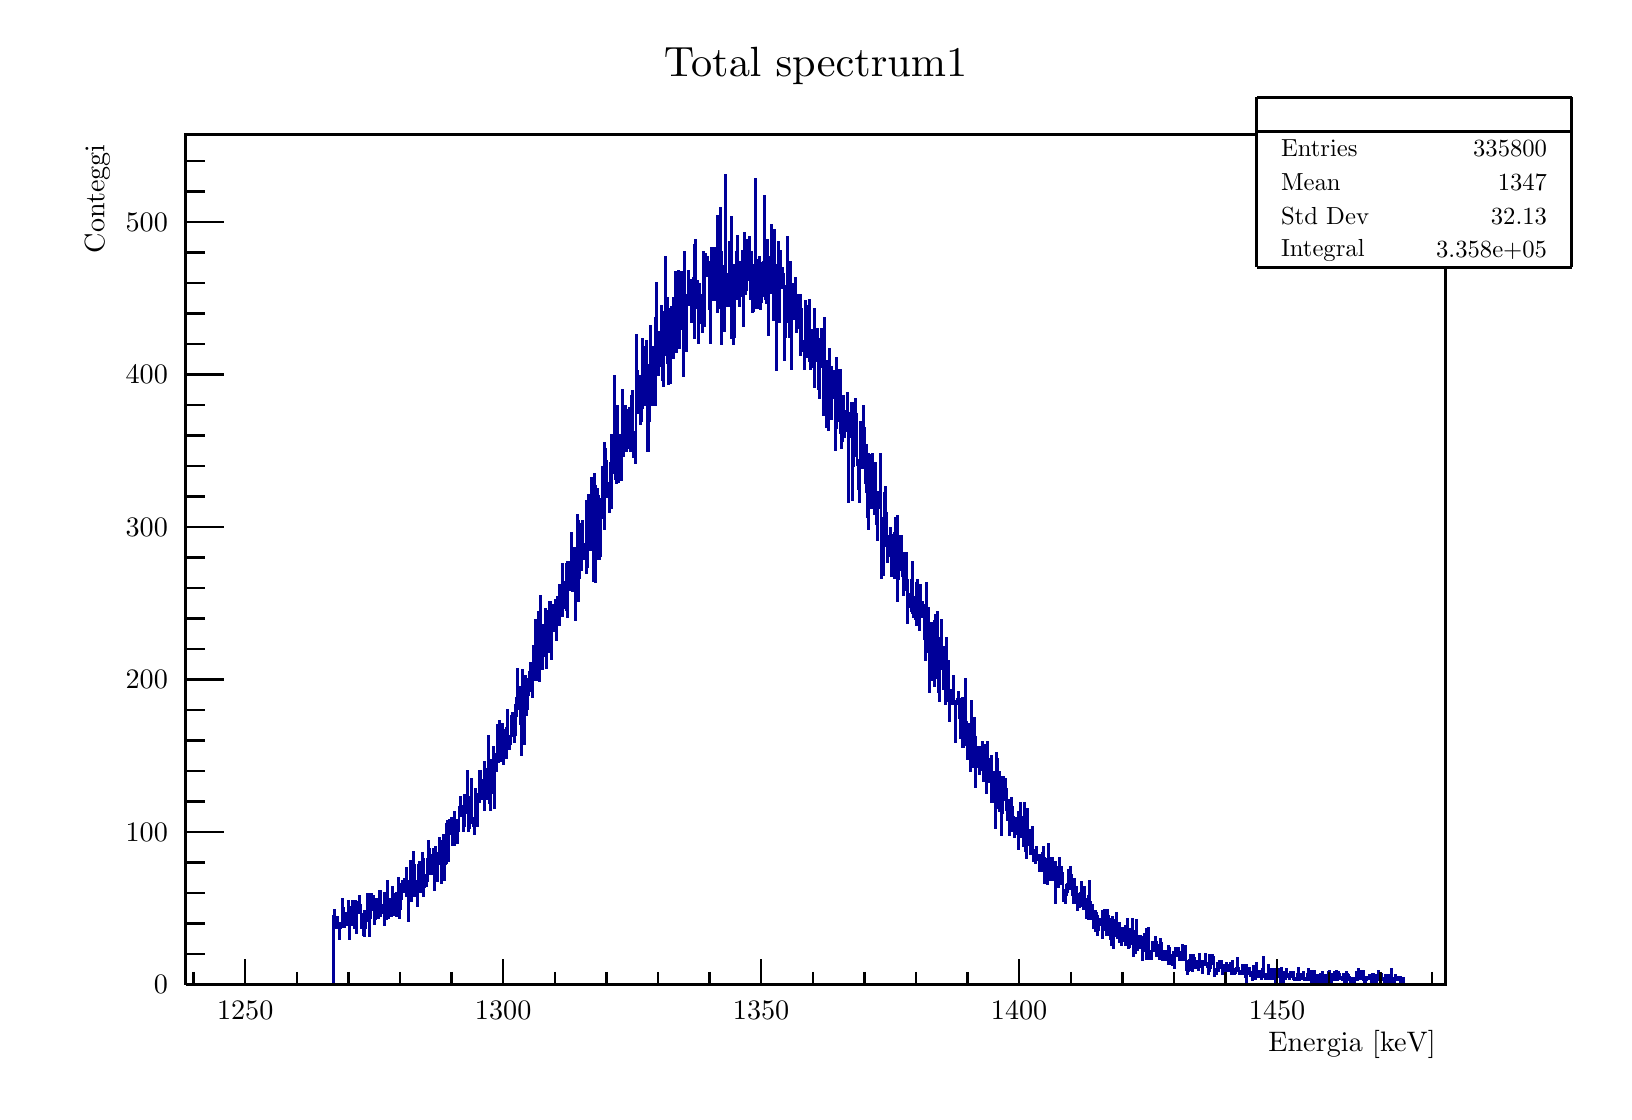
\begin{tikzpicture}
\pgfdeclareplotmark{cross} {
\pgfpathmoveto{\pgfpoint{-0.3\pgfplotmarksize}{\pgfplotmarksize}}
\pgfpathlineto{\pgfpoint{+0.3\pgfplotmarksize}{\pgfplotmarksize}}
\pgfpathlineto{\pgfpoint{+0.3\pgfplotmarksize}{0.3\pgfplotmarksize}}
\pgfpathlineto{\pgfpoint{+1\pgfplotmarksize}{0.3\pgfplotmarksize}}
\pgfpathlineto{\pgfpoint{+1\pgfplotmarksize}{-0.3\pgfplotmarksize}}
\pgfpathlineto{\pgfpoint{+0.3\pgfplotmarksize}{-0.3\pgfplotmarksize}}
\pgfpathlineto{\pgfpoint{+0.3\pgfplotmarksize}{-1.\pgfplotmarksize}}
\pgfpathlineto{\pgfpoint{-0.3\pgfplotmarksize}{-1.\pgfplotmarksize}}
\pgfpathlineto{\pgfpoint{-0.3\pgfplotmarksize}{-0.3\pgfplotmarksize}}
\pgfpathlineto{\pgfpoint{-1.\pgfplotmarksize}{-0.3\pgfplotmarksize}}
\pgfpathlineto{\pgfpoint{-1.\pgfplotmarksize}{0.3\pgfplotmarksize}}
\pgfpathlineto{\pgfpoint{-0.3\pgfplotmarksize}{0.3\pgfplotmarksize}}
\pgfpathclose
\pgfusepathqstroke
}
\pgfdeclareplotmark{cross*} {
\pgfpathmoveto{\pgfpoint{-0.3\pgfplotmarksize}{\pgfplotmarksize}}
\pgfpathlineto{\pgfpoint{+0.3\pgfplotmarksize}{\pgfplotmarksize}}
\pgfpathlineto{\pgfpoint{+0.3\pgfplotmarksize}{0.3\pgfplotmarksize}}
\pgfpathlineto{\pgfpoint{+1\pgfplotmarksize}{0.3\pgfplotmarksize}}
\pgfpathlineto{\pgfpoint{+1\pgfplotmarksize}{-0.3\pgfplotmarksize}}
\pgfpathlineto{\pgfpoint{+0.3\pgfplotmarksize}{-0.3\pgfplotmarksize}}
\pgfpathlineto{\pgfpoint{+0.3\pgfplotmarksize}{-1.\pgfplotmarksize}}
\pgfpathlineto{\pgfpoint{-0.3\pgfplotmarksize}{-1.\pgfplotmarksize}}
\pgfpathlineto{\pgfpoint{-0.3\pgfplotmarksize}{-0.3\pgfplotmarksize}}
\pgfpathlineto{\pgfpoint{-1.\pgfplotmarksize}{-0.3\pgfplotmarksize}}
\pgfpathlineto{\pgfpoint{-1.\pgfplotmarksize}{0.3\pgfplotmarksize}}
\pgfpathlineto{\pgfpoint{-0.3\pgfplotmarksize}{0.3\pgfplotmarksize}}
\pgfpathclose
\pgfusepathqfillstroke
}
\pgfdeclareplotmark{newstar} {
\pgfpathmoveto{\pgfqpoint{0pt}{\pgfplotmarksize}}
\pgfpathlineto{\pgfqpointpolar{44}{0.5\pgfplotmarksize}}
\pgfpathlineto{\pgfqpointpolar{18}{\pgfplotmarksize}}
\pgfpathlineto{\pgfqpointpolar{-20}{0.5\pgfplotmarksize}}
\pgfpathlineto{\pgfqpointpolar{-54}{\pgfplotmarksize}}
\pgfpathlineto{\pgfqpointpolar{-90}{0.5\pgfplotmarksize}}
\pgfpathlineto{\pgfqpointpolar{234}{\pgfplotmarksize}}
\pgfpathlineto{\pgfqpointpolar{198}{0.5\pgfplotmarksize}}
\pgfpathlineto{\pgfqpointpolar{162}{\pgfplotmarksize}}
\pgfpathlineto{\pgfqpointpolar{134}{0.5\pgfplotmarksize}}
\pgfpathclose
\pgfusepathqstroke
}
\pgfdeclareplotmark{newstar*} {
\pgfpathmoveto{\pgfqpoint{0pt}{\pgfplotmarksize}}
\pgfpathlineto{\pgfqpointpolar{44}{0.5\pgfplotmarksize}}
\pgfpathlineto{\pgfqpointpolar{18}{\pgfplotmarksize}}
\pgfpathlineto{\pgfqpointpolar{-20}{0.5\pgfplotmarksize}}
\pgfpathlineto{\pgfqpointpolar{-54}{\pgfplotmarksize}}
\pgfpathlineto{\pgfqpointpolar{-90}{0.5\pgfplotmarksize}}
\pgfpathlineto{\pgfqpointpolar{234}{\pgfplotmarksize}}
\pgfpathlineto{\pgfqpointpolar{198}{0.5\pgfplotmarksize}}
\pgfpathlineto{\pgfqpointpolar{162}{\pgfplotmarksize}}
\pgfpathlineto{\pgfqpointpolar{134}{0.5\pgfplotmarksize}}
\pgfpathclose
\pgfusepathqfillstroke
}
\definecolor{c}{rgb}{1,1,1};
\draw [color=c, fill=c] (0,0) rectangle (20,13.4957);
\draw [color=c, fill=c] (2,1.34957) rectangle (18,12.1461);
\definecolor{c}{rgb}{0,0,0};
\draw [c,line width=0.9] (2,1.34957) -- (2,12.1461) -- (18,12.1461) -- (18,1.34957) -- (2,1.34957);
\definecolor{c}{rgb}{1,1,1};
\draw [color=c, fill=c] (2,1.34957) rectangle (18,12.1461);
\definecolor{c}{rgb}{0,0,0};
\draw [c,line width=0.9] (2,1.34957) -- (2,12.1461) -- (18,12.1461) -- (18,1.34957) -- (2,1.34957);
\definecolor{c}{rgb}{0,0,0.6};
\draw [c,line width=0.9] (2,1.34957) -- (2.00716,1.34957) -- (2.00716,1.34957) -- (2.01431,1.34957) -- (2.01431,1.34957) -- (2.02147,1.34957) -- (2.02147,1.34957) -- (2.02862,1.34957) -- (2.02862,1.34957) -- (2.03578,1.34957) -- (2.03578,1.34957) --
 (2.04293,1.34957) -- (2.04293,1.34957) -- (2.05009,1.34957) -- (2.05009,1.34957) -- (2.05725,1.34957) -- (2.05725,1.34957) -- (2.0644,1.34957) -- (2.0644,1.34957) -- (2.07156,1.34957) -- (2.07156,1.34957) -- (2.07871,1.34957) -- (2.07871,1.34957) --
 (2.08587,1.34957) -- (2.08587,1.34957) -- (2.09302,1.34957) -- (2.09302,1.34957) -- (2.10018,1.34957) -- (2.10018,1.34957) -- (2.10733,1.34957) -- (2.10733,1.34957) -- (2.11449,1.34957) -- (2.11449,1.34957) -- (2.12165,1.34957) -- (2.12165,1.34957)
 -- (2.1288,1.34957) -- (2.1288,1.34957) -- (2.13596,1.34957) -- (2.13596,1.34957) -- (2.14311,1.34957) -- (2.14311,1.34957) -- (2.15027,1.34957) -- (2.15027,1.34957) -- (2.15742,1.34957) -- (2.15742,1.34957) -- (2.16458,1.34957) -- (2.16458,1.34957)
 -- (2.17174,1.34957) -- (2.17174,1.34957) -- (2.17889,1.34957) -- (2.17889,1.34957) -- (2.18605,1.34957) -- (2.18605,1.34957) -- (2.1932,1.34957) -- (2.1932,1.34957) -- (2.20036,1.34957) -- (2.20036,1.34957) -- (2.20751,1.34957) -- (2.20751,1.34957)
 -- (2.21467,1.34957) -- (2.21467,1.34957) -- (2.22182,1.34957) -- (2.22182,1.34957) -- (2.22898,1.34957) -- (2.22898,1.34957) -- (2.23614,1.34957) -- (2.23614,1.34957) -- (2.24329,1.34957) -- (2.24329,1.34957) -- (2.25045,1.34957) --
 (2.25045,1.34957) -- (2.2576,1.34957) -- (2.2576,1.34957) -- (2.26476,1.34957) -- (2.26476,1.34957) -- (2.27191,1.34957) -- (2.27191,1.34957) -- (2.27907,1.34957) -- (2.27907,1.34957) -- (2.28623,1.34957) -- (2.28623,1.34957) -- (2.29338,1.34957) --
 (2.29338,1.34957) -- (2.30054,1.34957) -- (2.30054,1.34957) -- (2.30769,1.34957) -- (2.30769,1.34957) -- (2.31485,1.34957) -- (2.31485,1.34957) -- (2.322,1.34957) -- (2.322,1.34957) -- (2.32916,1.34957) -- (2.32916,1.34957) -- (2.33631,1.34957) --
 (2.33631,1.34957) -- (2.34347,1.34957) -- (2.34347,1.34957) -- (2.35063,1.34957) -- (2.35063,1.34957) -- (2.35778,1.34957) -- (2.35778,1.34957) -- (2.36494,1.34957) -- (2.36494,1.34957) -- (2.37209,1.34957) -- (2.37209,1.34957) -- (2.37925,1.34957)
 -- (2.37925,1.34957) -- (2.3864,1.34957) -- (2.3864,1.34957) -- (2.39356,1.34957) -- (2.39356,1.34957) -- (2.40072,1.34957) -- (2.40072,1.34957) -- (2.40787,1.34957) -- (2.40787,1.34957) -- (2.41503,1.34957) -- (2.41503,1.34957) -- (2.42218,1.34957)
 -- (2.42218,1.34957) -- (2.42934,1.34957) -- (2.42934,1.34957) -- (2.43649,1.34957) -- (2.43649,1.34957) -- (2.44365,1.34957) -- (2.44365,1.34957) -- (2.45081,1.34957) -- (2.45081,1.34957) -- (2.45796,1.34957) -- (2.45796,1.34957) --
 (2.46512,1.34957) -- (2.46512,1.34957) -- (2.47227,1.34957) -- (2.47227,1.34957) -- (2.47943,1.34957) -- (2.47943,1.34957) -- (2.48658,1.34957) -- (2.48658,1.34957) -- (2.49374,1.34957) -- (2.49374,1.34957) -- (2.50089,1.34957) -- (2.50089,1.34957)
 -- (2.50805,1.34957) -- (2.50805,1.34957) -- (2.51521,1.34957) -- (2.51521,1.34957) -- (2.52236,1.34957) -- (2.52236,1.34957) -- (2.52952,1.34957) -- (2.52952,1.34957) -- (2.53667,1.34957) -- (2.53667,1.34957) -- (2.54383,1.34957) --
 (2.54383,1.34957) -- (2.55098,1.34957) -- (2.55098,1.34957) -- (2.55814,1.34957) -- (2.55814,1.34957) -- (2.5653,1.34957) -- (2.5653,1.34957) -- (2.57245,1.34957) -- (2.57245,1.34957) -- (2.57961,1.34957) -- (2.57961,1.34957) -- (2.58676,1.34957) --
 (2.58676,1.34957) -- (2.59392,1.34957) -- (2.59392,1.34957) -- (2.60107,1.34957) -- (2.60107,1.34957) -- (2.60823,1.34957) -- (2.60823,1.34957) -- (2.61538,1.34957) -- (2.61538,1.34957) -- (2.62254,1.34957) -- (2.62254,1.34957) -- (2.6297,1.34957)
 -- (2.6297,1.34957) -- (2.63685,1.34957) -- (2.63685,1.34957) -- (2.64401,1.34957) -- (2.64401,1.34957) -- (2.65116,1.34957) -- (2.65116,1.34957) -- (2.65832,1.34957) -- (2.65832,1.34957) -- (2.66547,1.34957) -- (2.66547,1.34957) --
 (2.67263,1.34957) -- (2.67263,1.34957) -- (2.67979,1.34957) -- (2.67979,1.34957) -- (2.68694,1.34957) -- (2.68694,1.34957) -- (2.6941,1.34957) -- (2.6941,1.34957) -- (2.70125,1.34957) -- (2.70125,1.34957) -- (2.70841,1.34957) -- (2.70841,1.34957) --
 (2.71556,1.34957) -- (2.71556,1.34957) -- (2.72272,1.34957) -- (2.72272,1.34957) -- (2.72987,1.34957) -- (2.72987,1.34957) -- (2.73703,1.34957) -- (2.73703,1.34957) -- (2.74419,1.34957) -- (2.74419,1.34957) -- (2.75134,1.34957) -- (2.75134,1.34957)
 -- (2.7585,1.34957) -- (2.7585,1.34957) -- (2.76565,1.34957) -- (2.76565,1.34957) -- (2.77281,1.34957) -- (2.77281,1.34957) -- (2.77996,1.34957) -- (2.77996,1.34957) -- (2.78712,1.34957) -- (2.78712,1.34957) -- (2.79428,1.34957) -- (2.79428,1.34957)
 -- (2.80143,1.34957) -- (2.80143,1.34957) -- (2.80859,1.34957) -- (2.80859,1.34957) -- (2.81574,1.34957) -- (2.81574,1.34957) -- (2.8229,1.34957) -- (2.8229,1.34957) -- (2.83005,1.34957) -- (2.83005,1.34957) -- (2.83721,1.34957) -- (2.83721,1.34957)
 -- (2.84437,1.34957) -- (2.84437,1.34957) -- (2.85152,1.34957) -- (2.85152,1.34957) -- (2.85868,1.34957) -- (2.85868,1.34957) -- (2.86583,1.34957) -- (2.86583,1.34957) -- (2.87299,1.34957) -- (2.87299,1.34957) -- (2.88014,1.34957) --
 (2.88014,1.34957) -- (2.8873,1.34957) -- (2.8873,1.34957) -- (2.89445,1.34957) -- (2.89445,1.34957) -- (2.90161,1.34957) -- (2.90161,1.34957) -- (2.90877,1.34957) -- (2.90877,1.34957) -- (2.91592,1.34957) -- (2.91592,1.34957) -- (2.92308,1.34957) --
 (2.92308,1.34957) -- (2.93023,1.34957) -- (2.93023,1.34957) -- (2.93739,1.34957) -- (2.93739,1.34957) -- (2.94454,1.34957) -- (2.94454,1.34957) -- (2.9517,1.34957) -- (2.9517,1.34957) -- (2.95886,1.34957) -- (2.95886,1.34957) -- (2.96601,1.34957) --
 (2.96601,1.34957) -- (2.97317,1.34957) -- (2.97317,1.34957) -- (2.98032,1.34957) -- (2.98032,1.34957) -- (2.98748,1.34957) -- (2.98748,1.34957) -- (2.99463,1.34957) -- (2.99463,1.34957) -- (3.00179,1.34957) -- (3.00179,1.34957) -- (3.00894,1.34957)
 -- (3.00894,1.34957) -- (3.0161,1.34957) -- (3.0161,1.34957) -- (3.02326,1.34957) -- (3.02326,1.34957) -- (3.03041,1.34957) -- (3.03041,1.34957) -- (3.03757,1.34957) -- (3.03757,1.34957) -- (3.04472,1.34957) -- (3.04472,1.34957) -- (3.05188,1.34957)
 -- (3.05188,1.34957) -- (3.05903,1.34957) -- (3.05903,1.34957) -- (3.06619,1.34957) -- (3.06619,1.34957) -- (3.07335,1.34957) -- (3.07335,1.34957) -- (3.0805,1.34957) -- (3.0805,1.34957) -- (3.08766,1.34957) -- (3.08766,1.34957) -- (3.09481,1.34957)
 -- (3.09481,1.34957) -- (3.10197,1.34957) -- (3.10197,1.34957) -- (3.10912,1.34957) -- (3.10912,1.34957) -- (3.11628,1.34957) -- (3.11628,1.34957) -- (3.12343,1.34957) -- (3.12343,1.34957) -- (3.13059,1.34957) -- (3.13059,1.34957) --
 (3.13775,1.34957) -- (3.13775,1.34957) -- (3.1449,1.34957) -- (3.1449,1.34957) -- (3.15206,1.34957) -- (3.15206,1.34957) -- (3.15921,1.34957) -- (3.15921,1.34957) -- (3.16637,1.34957) -- (3.16637,1.34957) -- (3.17352,1.34957) -- (3.17352,1.34957) --
 (3.18068,1.34957) -- (3.18068,1.34957) -- (3.18784,1.34957) -- (3.18784,1.34957) -- (3.19499,1.34957) -- (3.19499,1.34957) -- (3.20215,1.34957) -- (3.20215,1.34957) -- (3.2093,1.34957) -- (3.2093,1.34957) -- (3.21646,1.34957) -- (3.21646,1.34957) --
 (3.22361,1.34957) -- (3.22361,1.34957) -- (3.23077,1.34957) -- (3.23077,1.34957) -- (3.23793,1.34957) -- (3.23793,1.34957) -- (3.24508,1.34957) -- (3.24508,1.34957) -- (3.25224,1.34957) -- (3.25224,1.34957) -- (3.25939,1.34957) -- (3.25939,1.34957)
 -- (3.26655,1.34957) -- (3.26655,1.34957) -- (3.2737,1.34957) -- (3.2737,1.34957) -- (3.28086,1.34957) -- (3.28086,1.34957) -- (3.28801,1.34957) -- (3.28801,1.34957) -- (3.29517,1.34957) -- (3.29517,1.34957) -- (3.30233,1.34957) -- (3.30233,1.34957)
 -- (3.30948,1.34957) -- (3.30948,1.34957) -- (3.31664,1.34957) -- (3.31664,1.34957) -- (3.32379,1.34957) -- (3.32379,1.34957) -- (3.33095,1.34957) -- (3.33095,1.34957) -- (3.3381,1.34957) -- (3.3381,1.34957) -- (3.34526,1.34957) -- (3.34526,1.34957)
 -- (3.35242,1.34957) -- (3.35242,1.34957) -- (3.35957,1.34957) -- (3.35957,1.34957) -- (3.36673,1.34957) -- (3.36673,1.34957) -- (3.37388,1.34957) -- (3.37388,1.34957) -- (3.38104,1.34957) -- (3.38104,1.34957) -- (3.38819,1.34957) --
 (3.38819,1.34957) -- (3.39535,1.34957) -- (3.39535,1.34957) -- (3.4025,1.34957) -- (3.4025,1.34957) -- (3.40966,1.34957) -- (3.40966,1.34957) -- (3.41682,1.34957) -- (3.41682,1.34957) -- (3.42397,1.34957) -- (3.42397,1.34957) -- (3.43113,1.34957) --
 (3.43113,1.34957) -- (3.43828,1.34957) -- (3.43828,1.34957) -- (3.44544,1.34957) -- (3.44544,1.34957) -- (3.45259,1.34957) -- (3.45259,1.34957) -- (3.45975,1.34957) -- (3.45975,1.34957) -- (3.46691,1.34957) -- (3.46691,1.34957) -- (3.47406,1.34957)
 -- (3.47406,1.34957) -- (3.48122,1.34957) -- (3.48122,1.34957) -- (3.48837,1.34957) -- (3.48837,1.34957) -- (3.49553,1.34957) -- (3.49553,1.34957) -- (3.50268,1.34957) -- (3.50268,1.34957) -- (3.50984,1.34957) -- (3.50984,1.34957) --
 (3.51699,1.34957) -- (3.51699,1.34957) -- (3.52415,1.34957) -- (3.52415,1.34957) -- (3.53131,1.34957) -- (3.53131,1.34957) -- (3.53846,1.34957) -- (3.53846,1.34957) -- (3.54562,1.34957) -- (3.54562,1.34957) -- (3.55277,1.34957) -- (3.55277,1.34957)
 -- (3.55993,1.34957) -- (3.55993,1.34957) -- (3.56708,1.34957) -- (3.56708,1.34957) -- (3.57424,1.34957) -- (3.57424,1.34957) -- (3.5814,1.34957) -- (3.5814,1.34957) -- (3.58855,1.34957) -- (3.58855,1.34957) -- (3.59571,1.34957) -- (3.59571,1.34957)
 -- (3.60286,1.34957) -- (3.60286,1.34957) -- (3.61002,1.34957) -- (3.61002,1.34957) -- (3.61717,1.34957) -- (3.61717,1.34957) -- (3.62433,1.34957) -- (3.62433,1.34957) -- (3.63148,1.34957) -- (3.63148,1.34957) -- (3.63864,1.34957) --
 (3.63864,1.34957) -- (3.6458,1.34957) -- (3.6458,1.34957) -- (3.65295,1.34957) -- (3.65295,1.34957) -- (3.66011,1.34957) -- (3.66011,1.34957) -- (3.66726,1.34957) -- (3.66726,1.34957) -- (3.67442,1.34957) -- (3.67442,1.34957) -- (3.68157,1.34957) --
 (3.68157,1.34957) -- (3.68873,1.34957) -- (3.68873,1.34957) -- (3.69589,1.34957) -- (3.69589,1.34957) -- (3.70304,1.34957) -- (3.70304,1.34957) -- (3.7102,1.34957) -- (3.7102,1.34957) -- (3.71735,1.34957) -- (3.71735,1.34957) -- (3.72451,1.34957) --
 (3.72451,1.34957) -- (3.73166,1.34957) -- (3.73166,1.34957) -- (3.73882,1.34957) -- (3.73882,1.34957) -- (3.74598,1.34957) -- (3.74598,1.34957) -- (3.75313,1.34957) -- (3.75313,1.34957) -- (3.76029,1.34957) -- (3.76029,1.34957) -- (3.76744,1.34957)
 -- (3.76744,1.34957) -- (3.7746,1.34957) -- (3.7746,1.34957) -- (3.78175,1.34957) -- (3.78175,1.34957) -- (3.78891,1.34957) -- (3.78891,1.34957) -- (3.79606,1.34957) -- (3.79606,1.34957) -- (3.80322,1.34957) -- (3.80322,1.34957) -- (3.81038,1.34957)
 -- (3.81038,1.34957) -- (3.81753,1.34957) -- (3.81753,1.34957) -- (3.82469,1.34957) -- (3.82469,1.34957) -- (3.83184,1.34957) -- (3.83184,1.34957) -- (3.839,1.34957) -- (3.839,1.34957) -- (3.84615,1.34957) -- (3.84615,1.34957) -- (3.85331,1.34957)
 -- (3.85331,1.34957) -- (3.86047,1.34957) -- (3.86047,1.34957) -- (3.86762,1.34957) -- (3.86762,1.34957) -- (3.87478,1.34957) -- (3.87478,2.22096) -- (3.88193,2.22096) -- (3.88193,2.08541) -- (3.88909,2.08541) -- (3.88909,2.29842) --
 (3.89624,2.29842) -- (3.89624,2.06605) -- (3.9034,2.06605) -- (3.9034,2.18223) -- (3.91055,2.18223) -- (3.91055,2.18223) -- (3.91771,2.18223) -- (3.91771,2.2016) -- (3.92487,2.2016) -- (3.92487,2.12414) -- (3.93202,2.12414) -- (3.93202,2.06605) --
 (3.93918,2.06605) -- (3.93918,2.06605) -- (3.94633,2.06605) -- (3.94633,1.9305) -- (3.95349,1.9305) -- (3.95349,2.10478) -- (3.96064,2.10478) -- (3.96064,2.12414) -- (3.9678,2.12414) -- (3.9678,2.06605) -- (3.97496,2.06605) -- (3.97496,2.08541) --
 (3.98211,2.08541) -- (3.98211,2.12414) -- (3.98927,2.12414) -- (3.98927,2.43397) -- (3.99642,2.43397) -- (3.99642,2.29842) -- (4.00358,2.29842) -- (4.00358,2.31778) -- (4.01073,2.31778) -- (4.01073,2.08541) -- (4.01789,2.08541) -- (4.01789,2.18223)
 -- (4.02504,2.18223) -- (4.02504,2.25969) -- (4.0322,2.25969) -- (4.0322,2.2016) -- (4.03936,2.2016) -- (4.03936,2.12414) -- (4.04651,2.12414) -- (4.04651,2.14351) -- (4.05367,2.14351) -- (4.05367,2.10478) -- (4.06082,2.10478) -- (4.06082,2.18223)
 -- (4.06798,2.18223) -- (4.06798,2.41461) -- (4.07513,2.41461) -- (4.07513,1.9305) -- (4.08229,1.9305) -- (4.08229,2.16287) -- (4.08945,2.16287) -- (4.08945,2.27906) -- (4.0966,2.27906) -- (4.0966,2.33715) -- (4.10376,2.33715) -- (4.10376,2.29842)
 -- (4.11091,2.29842) -- (4.11091,2.41461) -- (4.11807,2.41461) -- (4.11807,2.10478) -- (4.12522,2.10478) -- (4.12522,2.35651) -- (4.13238,2.35651) -- (4.13238,2.31778) -- (4.13953,2.31778) -- (4.13953,2.06605) -- (4.14669,2.06605) --
 (4.14669,2.16287) -- (4.15385,2.16287) -- (4.15385,2.41461) -- (4.161,2.41461) -- (4.161,2.00796) -- (4.16816,2.00796) -- (4.16816,2.10478) -- (4.17531,2.10478) -- (4.17531,2.27906) -- (4.18247,2.27906) -- (4.18247,2.33715) -- (4.18962,2.33715) --
 (4.18962,2.25969) -- (4.19678,2.25969) -- (4.19678,2.39524) -- (4.20394,2.39524) -- (4.20394,2.4727) -- (4.21109,2.4727) -- (4.21109,2.35651) -- (4.21825,2.35651) -- (4.21825,2.33715) -- (4.2254,2.33715) -- (4.2254,2.24033) -- (4.23256,2.24033) --
 (4.23256,2.06605) -- (4.23971,2.06605) -- (4.23971,2.2016) -- (4.24687,2.2016) -- (4.24687,2.18223) -- (4.25402,2.18223) -- (4.25402,1.98859) -- (4.26118,1.98859) -- (4.26118,2.27906) -- (4.26834,2.27906) -- (4.26834,1.96923) -- (4.27549,1.96923) --
 (4.27549,2.06605) -- (4.28265,2.06605) -- (4.28265,2.14351) -- (4.2898,2.14351) -- (4.2898,2.16287) -- (4.29696,2.16287) -- (4.29696,2.22096) -- (4.30411,2.22096) -- (4.30411,2.18223) -- (4.31127,2.18223) -- (4.31127,2.49206) -- (4.31843,2.49206) --
 (4.31843,2.25969) -- (4.32558,2.25969) -- (4.32558,1.96923) -- (4.33274,1.96923) -- (4.33274,2.39524) -- (4.33989,2.39524) -- (4.33989,2.24033) -- (4.34705,2.24033) -- (4.34705,2.2016) -- (4.3542,2.2016) -- (4.3542,2.49206) -- (4.36136,2.49206) --
 (4.36136,2.35651) -- (4.36852,2.35651) -- (4.36852,2.29842) -- (4.37567,2.29842) -- (4.37567,2.4727) -- (4.38283,2.4727) -- (4.38283,2.31778) -- (4.38998,2.31778) -- (4.38998,2.39524) -- (4.39714,2.39524) -- (4.39714,2.12414) -- (4.40429,2.12414) --
 (4.40429,2.31778) -- (4.41145,2.31778) -- (4.41145,2.18223) -- (4.4186,2.18223) -- (4.4186,2.43397) -- (4.42576,2.43397) -- (4.42576,2.35651) -- (4.43292,2.35651) -- (4.43292,2.33715) -- (4.44007,2.33715) -- (4.44007,2.2016) -- (4.44723,2.2016) --
 (4.44723,2.24033) -- (4.45438,2.24033) -- (4.45438,2.24033) -- (4.46154,2.24033) -- (4.46154,2.53079) -- (4.46869,2.53079) -- (4.46869,2.53079) -- (4.47585,2.53079) -- (4.47585,2.22096) -- (4.48301,2.22096) -- (4.48301,2.31778) -- (4.49016,2.31778)
 -- (4.49016,2.35651) -- (4.49732,2.35651) -- (4.49732,2.31778) -- (4.50447,2.31778) -- (4.50447,2.35651) -- (4.51163,2.35651) -- (4.51163,2.25969) -- (4.51878,2.25969) -- (4.51878,2.51143) -- (4.52594,2.51143) -- (4.52594,2.10478) --
 (4.53309,2.10478) -- (4.53309,2.45334) -- (4.54025,2.45334) -- (4.54025,2.18223) -- (4.54741,2.18223) -- (4.54741,2.18223) -- (4.55456,2.18223) -- (4.55456,2.49206) -- (4.56172,2.49206) -- (4.56172,2.66634) -- (4.56887,2.66634) -- (4.56887,2.27906)
 -- (4.57603,2.27906) -- (4.57603,2.2016) -- (4.58318,2.2016) -- (4.58318,2.27906) -- (4.59034,2.27906) -- (4.59034,2.29842) -- (4.5975,2.29842) -- (4.5975,2.43397) -- (4.60465,2.43397) -- (4.60465,2.33715) -- (4.61181,2.33715) -- (4.61181,2.22096)
 -- (4.61896,2.22096) -- (4.61896,2.56952) -- (4.62612,2.56952) -- (4.62612,2.58889) -- (4.63327,2.58889) -- (4.63327,2.45334) -- (4.64043,2.45334) -- (4.64043,2.33715) -- (4.64758,2.33715) -- (4.64758,2.24033) -- (4.65474,2.24033) --
 (4.65474,2.4727) -- (4.6619,2.4727) -- (4.6619,2.49206) -- (4.66905,2.49206) -- (4.66905,2.22096) -- (4.67621,2.22096) -- (4.67621,2.51143) -- (4.68336,2.51143) -- (4.68336,2.4727) -- (4.69052,2.4727) -- (4.69052,2.31778) -- (4.69767,2.31778) --
 (4.69767,2.70507) -- (4.70483,2.70507) -- (4.70483,2.55016) -- (4.71199,2.55016) -- (4.71199,2.2016) -- (4.71914,2.2016) -- (4.71914,2.31778) -- (4.7263,2.31778) -- (4.7263,2.62761) -- (4.73345,2.62761) -- (4.73345,2.4727) -- (4.74061,2.4727) --
 (4.74061,2.43397) -- (4.74776,2.43397) -- (4.74776,2.53079) -- (4.75492,2.53079) -- (4.75492,2.66634) -- (4.76208,2.66634) -- (4.76208,2.58889) -- (4.76923,2.58889) -- (4.76923,2.55016) -- (4.77639,2.55016) -- (4.77639,2.68571) -- (4.78354,2.68571)
 -- (4.78354,2.53079) -- (4.7907,2.53079) -- (4.7907,2.64698) -- (4.79785,2.64698) -- (4.79785,2.82126) -- (4.80501,2.82126) -- (4.80501,2.4727) -- (4.81216,2.4727) -- (4.81216,2.66634) -- (4.81932,2.66634) -- (4.81932,2.4727) -- (4.82648,2.4727) --
 (4.82648,2.16287) -- (4.83363,2.16287) -- (4.83363,2.53079) -- (4.84079,2.53079) -- (4.84079,2.66634) -- (4.84794,2.66634) -- (4.84794,2.91808) -- (4.8551,2.91808) -- (4.8551,2.80189) -- (4.86225,2.80189) -- (4.86225,2.56952) -- (4.86941,2.56952) --
 (4.86941,2.41461) -- (4.87657,2.41461) -- (4.87657,2.58889) -- (4.88372,2.58889) -- (4.88372,2.68571) -- (4.89088,2.68571) -- (4.89088,3.03426) -- (4.89803,3.03426) -- (4.89803,2.85999) -- (4.90519,2.85999) -- (4.90519,2.4727) -- (4.91234,2.4727) --
 (4.91234,2.4727) -- (4.9195,2.4727) -- (4.9195,2.62761) -- (4.92665,2.62761) -- (4.92665,2.49206) -- (4.93381,2.49206) -- (4.93381,2.66634) -- (4.94097,2.66634) -- (4.94097,2.35651) -- (4.94812,2.35651) -- (4.94812,2.68571) -- (4.95528,2.68571) --
 (4.95528,2.85999) -- (4.96243,2.85999) -- (4.96243,2.53079) -- (4.96959,2.53079) -- (4.96959,2.89871) -- (4.97674,2.89871) -- (4.97674,2.53079) -- (4.9839,2.53079) -- (4.9839,2.82126) -- (4.99106,2.82126) -- (4.99106,2.72444) -- (4.99821,2.72444) --
 (4.99821,3.0149) -- (5.00537,3.0149) -- (5.00537,2.64698) -- (5.01252,2.64698) -- (5.01252,2.93744) -- (5.01968,2.93744) -- (5.01968,2.4727) -- (5.02683,2.4727) -- (5.02683,2.58889) -- (5.03399,2.58889) -- (5.03399,2.7438) -- (5.04114,2.7438) --
 (5.04114,2.70507) -- (5.0483,2.70507) -- (5.0483,2.7438) -- (5.05546,2.7438) -- (5.05546,2.60825) -- (5.06261,2.60825) -- (5.06261,2.66634) -- (5.06977,2.66634) -- (5.06977,2.93744) -- (5.07692,2.93744) -- (5.07692,3.16981) -- (5.08408,3.16981) --
 (5.08408,2.80189) -- (5.09123,2.80189) -- (5.09123,2.76316) -- (5.09839,2.76316) -- (5.09839,3.07299) -- (5.10555,3.07299) -- (5.10555,2.99554) -- (5.1127,2.99554) -- (5.1127,2.85999) -- (5.11986,2.85999) -- (5.11986,2.87935) -- (5.12701,2.87935) --
 (5.12701,2.76316) -- (5.13417,2.76316) -- (5.13417,2.84062) -- (5.14132,2.84062) -- (5.14132,2.87935) -- (5.14848,2.87935) -- (5.14848,3.07299) -- (5.15564,3.07299) -- (5.15564,2.55016) -- (5.16279,2.55016) -- (5.16279,3.09236) -- (5.16995,3.09236)
 -- (5.16995,2.99554) -- (5.1771,2.99554) -- (5.1771,2.80189) -- (5.18426,2.80189) -- (5.18426,2.80189) -- (5.19141,2.80189) -- (5.19141,3.0149) -- (5.19857,3.0149) -- (5.19857,2.66634) -- (5.20572,2.66634) -- (5.20572,2.95681) -- (5.21288,2.95681)
 -- (5.21288,2.87935) -- (5.22004,2.87935) -- (5.22004,3.20854) -- (5.22719,3.20854) -- (5.22719,2.99554) -- (5.23435,2.99554) -- (5.23435,3.16981) -- (5.2415,3.16981) -- (5.2415,2.64698) -- (5.24866,2.64698) -- (5.24866,2.99554) -- (5.25581,2.99554)
 -- (5.25581,3.03426) -- (5.26297,3.03426) -- (5.26297,3.09236) -- (5.27013,3.09236) -- (5.27013,3.24727) -- (5.27728,3.24727) -- (5.27728,2.68571) -- (5.28444,2.68571) -- (5.28444,2.97617) -- (5.29159,2.97617) -- (5.29159,2.87935) --
 (5.29875,2.87935) -- (5.29875,3.16981) -- (5.3059,3.16981) -- (5.3059,2.89871) -- (5.31306,2.89871) -- (5.31306,3.38282) -- (5.32021,3.38282) -- (5.32021,3.0149) -- (5.32737,3.0149) -- (5.32737,3.42155) -- (5.33453,3.42155) -- (5.33453,2.91808) --
 (5.34168,2.91808) -- (5.34168,3.44091) -- (5.34884,3.44091) -- (5.34884,3.26664) -- (5.35599,3.26664) -- (5.35599,3.40219) -- (5.36315,3.40219) -- (5.36315,3.40219) -- (5.3703,3.40219) -- (5.3703,3.42155) -- (5.37746,3.42155) -- (5.37746,3.46028) --
 (5.38462,3.46028) -- (5.38462,3.13109) -- (5.39177,3.13109) -- (5.39177,3.20854) -- (5.39893,3.20854) -- (5.39893,3.44091) -- (5.40608,3.44091) -- (5.40608,3.53774) -- (5.41324,3.53774) -- (5.41324,3.13109) -- (5.42039,3.13109) -- (5.42039,3.24727)
 -- (5.42755,3.24727) -- (5.42755,3.34409) -- (5.4347,3.34409) -- (5.4347,3.44091) -- (5.44186,3.44091) -- (5.44186,3.32473) -- (5.44902,3.32473) -- (5.44902,3.15045) -- (5.45617,3.15045) -- (5.45617,3.30536) -- (5.46333,3.30536) -- (5.46333,3.36346)
 -- (5.47048,3.36346) -- (5.47048,3.5571) -- (5.47764,3.5571) -- (5.47764,3.59583) -- (5.48479,3.59583) -- (5.48479,3.73138) -- (5.49195,3.73138) -- (5.49195,3.49901) -- (5.49911,3.49901) -- (5.49911,3.59583) -- (5.50626,3.59583) -- (5.50626,3.61519)
 -- (5.51342,3.61519) -- (5.51342,3.59583) -- (5.52057,3.59583) -- (5.52057,3.46028) -- (5.52773,3.46028) -- (5.52773,3.30536) -- (5.53488,3.30536) -- (5.53488,3.75074) -- (5.54204,3.75074) -- (5.54204,3.36346) -- (5.5492,3.36346) -- (5.5492,3.69265)
 -- (5.55635,3.69265) -- (5.55635,3.53774) -- (5.56351,3.53774) -- (5.56351,3.71201) -- (5.57066,3.71201) -- (5.57066,4.06057) -- (5.57782,4.06057) -- (5.57782,3.53774) -- (5.58497,3.53774) -- (5.58497,3.30536) -- (5.59213,3.30536) --
 (5.59213,3.73138) -- (5.59928,3.73138) -- (5.59928,3.34409) -- (5.60644,3.34409) -- (5.60644,3.46028) -- (5.6136,3.46028) -- (5.6136,3.49901) -- (5.62075,3.49901) -- (5.62075,3.96375) -- (5.62791,3.96375) -- (5.62791,3.61519) -- (5.63506,3.61519) --
 (5.63506,3.46028) -- (5.64222,3.46028) -- (5.64222,3.40219) -- (5.64937,3.40219) -- (5.64937,3.36346) -- (5.65653,3.36346) -- (5.65653,3.38282) -- (5.66369,3.38282) -- (5.66369,3.26664) -- (5.67084,3.26664) -- (5.67084,3.8282) -- (5.678,3.8282) --
 (5.678,3.63456) -- (5.68515,3.63456) -- (5.68515,3.40219) -- (5.69231,3.40219) -- (5.69231,3.57646) -- (5.69946,3.57646) -- (5.69946,3.75074) -- (5.70662,3.75074) -- (5.70662,3.36346) -- (5.71377,3.36346) -- (5.71377,3.77011) -- (5.72093,3.77011) --
 (5.72093,3.67329) -- (5.72809,3.67329) -- (5.72809,4.06057) -- (5.73524,4.06057) -- (5.73524,3.88629) -- (5.7424,3.88629) -- (5.7424,4.06057) -- (5.74955,4.06057) -- (5.74955,3.86693) -- (5.75671,3.86693) -- (5.75671,3.75074) -- (5.76386,3.75074) --
 (5.76386,3.88629) -- (5.77102,3.88629) -- (5.77102,3.71201) -- (5.77818,3.71201) -- (5.77818,3.94439) -- (5.78533,3.94439) -- (5.78533,4.17676) -- (5.79249,4.17676) -- (5.79249,3.57646) -- (5.79964,3.57646) -- (5.79964,3.88629) -- (5.8068,3.88629)
 -- (5.8068,3.86693) -- (5.81395,3.86693) -- (5.81395,3.84756) -- (5.82111,3.84756) -- (5.82111,3.71201) -- (5.82826,3.71201) -- (5.82826,4.07994) -- (5.83542,4.07994) -- (5.83542,3.88629) -- (5.84258,3.88629) -- (5.84258,4.50595) --
 (5.84973,4.50595) -- (5.84973,3.65392) -- (5.85689,3.65392) -- (5.85689,3.92502) -- (5.86404,3.92502) -- (5.86404,3.57646) -- (5.8712,3.57646) -- (5.8712,3.75074) -- (5.87835,3.75074) -- (5.87835,4.19612) -- (5.88551,4.19612) -- (5.88551,3.78947) --
 (5.89267,3.78947) -- (5.89267,4.11866) -- (5.89982,4.11866) -- (5.89982,4.06057) -- (5.90698,4.06057) -- (5.90698,4.3704) -- (5.91413,4.3704) -- (5.91413,4.27358) -- (5.92129,4.27358) -- (5.92129,3.59583) -- (5.92844,3.59583) -- (5.92844,4.13803) --
 (5.9356,4.13803) -- (5.9356,4.27358) -- (5.94275,4.27358) -- (5.94275,4.06057) -- (5.94991,4.06057) -- (5.94991,4.17676) -- (5.95707,4.17676) -- (5.95707,4.6415) -- (5.96422,4.6415) -- (5.96422,4.17676) -- (5.97138,4.17676) -- (5.97138,4.46722) --
 (5.97853,4.46722) -- (5.97853,4.52531) -- (5.98569,4.52531) -- (5.98569,4.69959) -- (5.99284,4.69959) -- (5.99284,4.35104) -- (6,4.35104) -- (6,4.3704) -- (6.00716,4.3704) -- (6.00716,4.19612) -- (6.01431,4.19612) -- (6.01431,4.40913) --
 (6.02147,4.40913) -- (6.02147,4.66086) -- (6.02862,4.66086) -- (6.02862,4.15739) -- (6.03578,4.15739) -- (6.03578,4.31231) -- (6.04293,4.31231) -- (6.04293,4.3704) -- (6.05009,4.3704) -- (6.05009,4.58341) -- (6.05725,4.58341) -- (6.05725,4.48659) --
 (6.0644,4.48659) -- (6.0644,4.60277) -- (6.07156,4.60277) -- (6.07156,4.23485) -- (6.07871,4.23485) -- (6.07871,4.83514) -- (6.08587,4.83514) -- (6.08587,4.3704) -- (6.09302,4.3704) -- (6.09302,4.44786) -- (6.10018,4.44786) -- (6.10018,4.50595) --
 (6.10733,4.50595) -- (6.10733,4.35104) -- (6.11449,4.35104) -- (6.11449,4.35104) -- (6.12165,4.35104) -- (6.12165,4.40913) -- (6.1288,4.40913) -- (6.1288,4.52531) -- (6.13596,4.52531) -- (6.13596,4.75769) -- (6.14311,4.75769) -- (6.14311,4.79641) --
 (6.15027,4.79641) -- (6.15027,4.68023) -- (6.15742,4.68023) -- (6.15742,4.50595) -- (6.16458,4.50595) -- (6.16458,4.75769) -- (6.17174,4.75769) -- (6.17174,4.42849) -- (6.17889,4.42849) -- (6.17889,4.52531) -- (6.18605,4.52531) -- (6.18605,4.89324)
 -- (6.1932,4.89324) -- (6.1932,4.99006) -- (6.20036,4.99006) -- (6.20036,4.75769) -- (6.20751,4.75769) -- (6.20751,5.35798) -- (6.21467,5.35798) -- (6.21467,4.87387) -- (6.22182,4.87387) -- (6.22182,5.04815) -- (6.22898,5.04815) -- (6.22898,4.85451)
 -- (6.23614,4.85451) -- (6.23614,5.06751) -- (6.24329,5.06751) -- (6.24329,4.66086) -- (6.25045,4.66086) -- (6.25045,5.12561) -- (6.2576,5.12561) -- (6.2576,5.04815) -- (6.26476,5.04815) -- (6.26476,4.27358) -- (6.27191,4.27358) -- (6.27191,4.60277)
 -- (6.27907,4.60277) -- (6.27907,5.33861) -- (6.28623,5.33861) -- (6.28623,4.95133) -- (6.29338,4.95133) -- (6.29338,5.00942) -- (6.30054,5.00942) -- (6.30054,4.40913) -- (6.30769,4.40913) -- (6.30769,5.00942) -- (6.31485,5.00942) --
 (6.31485,5.26116) -- (6.322,5.26116) -- (6.322,4.77705) -- (6.32916,4.77705) -- (6.32916,5.22243) -- (6.33631,5.22243) -- (6.33631,4.85451) -- (6.34347,4.85451) -- (6.34347,5.1837) -- (6.35063,5.1837) -- (6.35063,5.02879) -- (6.35778,5.02879) --
 (6.35778,5.24179) -- (6.36494,5.24179) -- (6.36494,5.31925) -- (6.37209,5.31925) -- (6.37209,5.41607) -- (6.37925,5.41607) -- (6.37925,5.43544) -- (6.3864,5.43544) -- (6.3864,5.43544) -- (6.39356,5.43544) -- (6.39356,5.08688) -- (6.40072,5.08688) --
 (6.40072,5.00942) -- (6.40787,5.00942) -- (6.40787,5.51289) -- (6.41503,5.51289) -- (6.41503,5.64844) -- (6.42218,5.64844) -- (6.42218,5.35798) -- (6.42934,5.35798) -- (6.42934,5.53226) -- (6.43649,5.53226) -- (6.43649,5.22243) -- (6.44365,5.22243)
 -- (6.44365,5.97764) -- (6.45081,5.97764) -- (6.45081,5.60971) -- (6.45796,5.60971) -- (6.45796,5.22243) -- (6.46512,5.22243) -- (6.46512,5.31925) -- (6.47227,5.31925) -- (6.47227,5.60971) -- (6.47943,5.60971) -- (6.47943,6.07446) --
 (6.48658,6.07446) -- (6.48658,5.20306) -- (6.49374,5.20306) -- (6.49374,5.4548) -- (6.50089,5.4548) -- (6.50089,5.64844) -- (6.50805,5.64844) -- (6.50805,6.28746) -- (6.51521,6.28746) -- (6.51521,5.80336) -- (6.52236,5.80336) -- (6.52236,5.35798) --
 (6.52952,5.35798) -- (6.52952,5.4548) -- (6.53667,5.4548) -- (6.53667,5.66781) -- (6.54383,5.66781) -- (6.54383,5.91954) -- (6.55098,5.91954) -- (6.55098,5.68717) -- (6.55814,5.68717) -- (6.55814,5.53226) -- (6.5653,5.53226) -- (6.5653,6.11319) --
 (6.57245,6.11319) -- (6.57245,5.37734) -- (6.57961,5.37734) -- (6.57961,5.70654) -- (6.58676,5.70654) -- (6.58676,5.93891) -- (6.59392,5.93891) -- (6.59392,5.78399) -- (6.60107,5.78399) -- (6.60107,5.57099) -- (6.60823,5.57099) -- (6.60823,6.09382)
 -- (6.61538,6.09382) -- (6.61538,5.88081) -- (6.62254,5.88081) -- (6.62254,6.21001) -- (6.6297,6.21001) -- (6.6297,5.82272) -- (6.63685,5.82272) -- (6.63685,5.97764) -- (6.64401,5.97764) -- (6.64401,5.49353) -- (6.65116,5.49353) -- (6.65116,6.17128)
 -- (6.65832,6.17128) -- (6.65832,5.93891) -- (6.66547,5.93891) -- (6.66547,5.84209) -- (6.67263,5.84209) -- (6.67263,6.09382) -- (6.67979,6.09382) -- (6.67979,6.01636) -- (6.68694,6.01636) -- (6.68694,6.01636) -- (6.6941,6.01636) -- (6.6941,6.22937)
 -- (6.70125,6.22937) -- (6.70125,5.7259) -- (6.70841,5.7259) -- (6.70841,5.76463) -- (6.71556,5.76463) -- (6.71556,5.91954) -- (6.72272,5.91954) -- (6.72272,6.2681) -- (6.72987,6.2681) -- (6.72987,5.997) -- (6.73703,5.997) -- (6.73703,5.91954) --
 (6.74419,5.91954) -- (6.74419,6.42302) -- (6.75134,6.42302) -- (6.75134,6.32619) -- (6.7585,6.32619) -- (6.7585,6.03573) -- (6.76565,6.03573) -- (6.76565,6.24874) -- (6.77281,6.24874) -- (6.77281,6.13255) -- (6.77996,6.13255) -- (6.77996,6.03573) --
 (6.78712,6.03573) -- (6.78712,6.69412) -- (6.79428,6.69412) -- (6.79428,6.38429) -- (6.80143,6.38429) -- (6.80143,6.13255) -- (6.80859,6.13255) -- (6.80859,6.21001) -- (6.81574,6.21001) -- (6.81574,6.28746) -- (6.8229,6.28746) -- (6.8229,6.46174) --
 (6.83005,6.46174) -- (6.83005,6.69412) -- (6.83721,6.69412) -- (6.83721,6.11319) -- (6.84437,6.11319) -- (6.84437,6.01636) -- (6.85152,6.01636) -- (6.85152,6.71348) -- (6.85868,6.71348) -- (6.85868,6.46174) -- (6.86583,6.46174) -- (6.86583,6.48111)
 -- (6.87299,6.48111) -- (6.87299,6.36492) -- (6.88014,6.36492) -- (6.88014,6.55857) -- (6.8873,6.55857) -- (6.8873,6.38429) -- (6.89445,6.38429) -- (6.89445,6.51984) -- (6.90161,6.51984) -- (6.90161,7.0814) -- (6.90877,7.0814) -- (6.90877,6.34556)
 -- (6.91592,6.34556) -- (6.91592,6.75221) -- (6.92308,6.75221) -- (6.92308,6.77157) -- (6.93023,6.77157) -- (6.93023,6.71348) -- (6.93739,6.71348) -- (6.93739,6.88776) -- (6.94454,6.88776) -- (6.94454,5.97764) -- (6.9517,5.97764) -- (6.9517,6.5392)
 -- (6.95886,6.5392) -- (6.95886,6.86839) -- (6.96601,6.86839) -- (6.96601,6.73284) -- (6.97317,6.73284) -- (6.97317,7.31377) -- (6.98032,7.31377) -- (6.98032,7.23632) -- (6.98748,7.23632) -- (6.98748,6.22937) -- (6.99463,6.22937) --
 (6.99463,6.73284) -- (7.00179,6.73284) -- (7.00179,6.51984) -- (7.00894,6.51984) -- (7.00894,7.19759) -- (7.0161,7.19759) -- (7.0161,7.12013) -- (7.02326,7.12013) -- (7.02326,6.61666) -- (7.03041,6.61666) -- (7.03041,6.98458) -- (7.03757,6.98458) --
 (7.03757,7.23632) -- (7.04472,7.23632) -- (7.04472,6.77157) -- (7.05188,6.77157) -- (7.05188,6.94585) -- (7.05903,6.94585) -- (7.05903,6.75221) -- (7.06619,6.75221) -- (7.06619,6.90712) -- (7.07335,6.90712) -- (7.07335,6.88776) -- (7.0805,6.88776)
 -- (7.0805,6.57793) -- (7.08766,6.57793) -- (7.08766,7.48805) -- (7.09481,7.48805) -- (7.09481,6.71348) -- (7.10197,6.71348) -- (7.10197,6.65539) -- (7.10912,6.65539) -- (7.10912,6.86839) -- (7.11628,6.86839) -- (7.11628,7.56551) --
 (7.12343,7.56551) -- (7.12343,7.52678) -- (7.13059,7.52678) -- (7.13059,6.86839) -- (7.13775,6.86839) -- (7.13775,7.31377) -- (7.1449,7.31377) -- (7.1449,7.77852) -- (7.15206,7.77852) -- (7.15206,7.23632) -- (7.15921,7.23632) -- (7.15921,7.41059) --
 (7.16637,7.41059) -- (7.16637,7.19759) -- (7.17352,7.19759) -- (7.17352,6.86839) -- (7.18068,6.86839) -- (7.18068,6.48111) -- (7.18784,6.48111) -- (7.18784,7.83661) -- (7.19499,7.83661) -- (7.19499,7.68169) -- (7.20215,7.68169) -- (7.20215,6.46174)
 -- (7.2093,6.46174) -- (7.2093,7.52678) -- (7.21646,7.52678) -- (7.21646,7.21695) -- (7.22361,7.21695) -- (7.22361,7.64297) -- (7.23077,7.64297) -- (7.23077,7.64297) -- (7.23793,7.64297) -- (7.23793,7.54614) -- (7.24508,7.54614) -- (7.24508,6.75221)
 -- (7.25224,6.75221) -- (7.25224,7.50742) -- (7.25939,7.50742) -- (7.25939,7.42996) -- (7.26655,7.42996) -- (7.26655,6.79094) -- (7.2737,6.79094) -- (7.2737,7.41059) -- (7.28086,7.41059) -- (7.28086,7.27504) -- (7.28801,7.27504) -- (7.28801,7.91407)
 -- (7.29517,7.91407) -- (7.29517,7.44932) -- (7.30233,7.44932) -- (7.30233,7.70106) -- (7.30948,7.70106) -- (7.30948,7.13949) -- (7.31664,7.13949) -- (7.31664,8.22389) -- (7.32379,8.22389) -- (7.32379,8.14644) -- (7.33095,8.14644) --
 (7.33095,7.6236) -- (7.3381,7.6236) -- (7.3381,7.85597) -- (7.34526,7.85597) -- (7.34526,7.99152) -- (7.35242,7.99152) -- (7.35242,7.72042) -- (7.35957,7.72042) -- (7.35957,7.54614) -- (7.36673,7.54614) -- (7.36673,7.66233) -- (7.37388,7.66233) --
 (7.37388,7.3525) -- (7.38104,7.3525) -- (7.38104,7.60424) -- (7.38819,7.60424) -- (7.38819,7.73979) -- (7.39535,7.73979) -- (7.39535,7.97216) -- (7.4025,7.97216) -- (7.4025,8.32072) -- (7.40966,8.32072) -- (7.40966,7.41059) -- (7.41682,7.41059) --
 (7.41682,7.85597) -- (7.42397,7.85597) -- (7.42397,8.32072) -- (7.43113,8.32072) -- (7.43113,7.91407) -- (7.43828,7.91407) -- (7.43828,9.07592) -- (7.44544,9.07592) -- (7.44544,8.28199) -- (7.45259,8.28199) -- (7.45259,8.4369) -- (7.45975,8.4369) --
 (7.45975,7.77852) -- (7.46691,7.77852) -- (7.46691,7.72042) -- (7.47406,7.72042) -- (7.47406,7.91407) -- (7.48122,7.91407) -- (7.48122,8.68864) -- (7.48837,8.68864) -- (7.48837,7.73979) -- (7.49553,7.73979) -- (7.49553,8.20453) -- (7.50268,8.20453)
 -- (7.50268,8.12707) -- (7.50984,8.12707) -- (7.50984,8.32072) -- (7.51699,8.32072) -- (7.51699,8.06898) -- (7.52415,8.06898) -- (7.52415,8.22389) -- (7.53131,8.22389) -- (7.53131,7.75915) -- (7.53846,7.75915) -- (7.53846,8.74673) --
 (7.54562,8.74673) -- (7.54562,8.90164) -- (7.55277,8.90164) -- (7.55277,8.06898) -- (7.55993,8.06898) -- (7.55993,8.10771) -- (7.56708,8.10771) -- (7.56708,8.61118) -- (7.57424,8.61118) -- (7.57424,8.51436) -- (7.5814,8.51436) -- (7.5814,8.68864) --
 (7.58855,8.68864) -- (7.58855,8.12707) -- (7.59571,8.12707) -- (7.59571,8.47563) -- (7.60286,8.47563) -- (7.60286,8.28199) -- (7.61002,8.28199) -- (7.61002,8.64991) -- (7.61717,8.64991) -- (7.61717,8.1658) -- (7.62433,8.1658) -- (7.62433,8.35944) --
 (7.63148,8.35944) -- (7.63148,8.66927) -- (7.63864,8.66927) -- (7.63864,8.51436) -- (7.6458,8.51436) -- (7.6458,8.12707) -- (7.65295,8.12707) -- (7.65295,8.34008) -- (7.66011,8.34008) -- (7.66011,8.82419) -- (7.66726,8.82419) -- (7.66726,8.88228) --
 (7.67442,8.88228) -- (7.67442,8.4369) -- (7.68157,8.4369) -- (7.68157,8.04962) -- (7.68873,8.04962) -- (7.68873,8.35944) -- (7.69589,8.35944) -- (7.69589,8.35944) -- (7.70304,8.35944) -- (7.70304,7.97216) -- (7.7102,7.97216) -- (7.7102,8.14644) --
 (7.71735,8.14644) -- (7.71735,9.59876) -- (7.72451,9.59876) -- (7.72451,9.11465) -- (7.73166,9.11465) -- (7.73166,8.63054) -- (7.73882,8.63054) -- (7.73882,9.13402) -- (7.74598,9.13402) -- (7.74598,8.92101) -- (7.75313,8.92101) -- (7.75313,8.61118)
 -- (7.76029,8.61118) -- (7.76029,9.07592) -- (7.76744,9.07592) -- (7.76744,8.47563) -- (7.7746,8.47563) -- (7.7746,8.82419) -- (7.78175,8.82419) -- (7.78175,8.51436) -- (7.78891,8.51436) -- (7.78891,8.53372) -- (7.79606,8.53372) -- (7.79606,8.66927)
 -- (7.80322,8.66927) -- (7.80322,9.54067) -- (7.81038,9.54067) -- (7.81038,8.94037) -- (7.81753,8.94037) -- (7.81753,8.708) -- (7.82469,8.708) -- (7.82469,9.01783) -- (7.83184,9.01783) -- (7.83184,9.44384) -- (7.839,9.44384) -- (7.839,9.07592) --
 (7.84615,9.07592) -- (7.84615,9.5213) -- (7.85331,9.5213) -- (7.85331,9.07592) -- (7.86047,9.07592) -- (7.86047,9.11465) -- (7.86762,9.11465) -- (7.86762,8.12707) -- (7.87478,8.12707) -- (7.87478,9.21147) -- (7.88193,9.21147) -- (7.88193,8.51436) --
 (7.88909,8.51436) -- (7.88909,8.66927) -- (7.89624,8.66927) -- (7.89624,9.71494) -- (7.9034,9.71494) -- (7.9034,8.99847) -- (7.91055,8.99847) -- (7.91055,9.13402) -- (7.91771,9.13402) -- (7.91771,9.36639) -- (7.92487,9.36639) -- (7.92487,8.708) --
 (7.93202,8.708) -- (7.93202,9.13402) -- (7.93918,9.13402) -- (7.93918,9.44384) -- (7.94633,9.44384) -- (7.94633,8.88228) -- (7.95349,8.88228) -- (7.95349,8.92101) -- (7.96064,8.92101) -- (7.96064,8.708) -- (7.9678,8.708) -- (7.9678,9.81177) --
 (7.97496,9.81177) -- (7.97496,10.2571) -- (7.98211,10.2571) -- (7.98211,9.13402) -- (7.98927,9.13402) -- (7.98927,9.30829) -- (7.99642,9.30829) -- (7.99642,9.63749) -- (8.00358,9.63749) -- (8.00358,9.09529) -- (8.01073,9.09529) -- (8.01073,9.40512)
 -- (8.01789,9.40512) -- (8.01789,9.21147) -- (8.02504,9.21147) -- (8.02504,9.26957) -- (8.0322,9.26957) -- (8.0322,9.40512) -- (8.03936,9.40512) -- (8.03936,9.96668) -- (8.04651,9.96668) -- (8.04651,9.54067) -- (8.05367,9.54067) -- (8.05367,9.03719)
 -- (8.06082,9.03719) -- (8.06082,8.95974) -- (8.06798,8.95974) -- (8.06798,9.15338) -- (8.07513,9.15338) -- (8.07513,9.42448) -- (8.08229,9.42448) -- (8.08229,9.88922) -- (8.08945,9.88922) -- (8.08945,10.5863) -- (8.0966,10.5863) -- (8.0966,9.77304)
 -- (8.10376,9.77304) -- (8.10376,9.34702) -- (8.11091,9.34702) -- (8.11091,9.2502) -- (8.11807,9.2502) -- (8.11807,10.0635) -- (8.12522,10.0635) -- (8.12522,9.67622) -- (8.13238,9.67622) -- (8.13238,8.9791) -- (8.13953,8.9791) -- (8.13953,9.92795)
 -- (8.14669,9.92795) -- (8.14669,8.99847) -- (8.15385,8.99847) -- (8.15385,9.81177) -- (8.161,9.81177) -- (8.161,9.94732) -- (8.16816,9.94732) -- (8.16816,9.50194) -- (8.17531,9.50194) -- (8.17531,9.54067) -- (8.18247,9.54067) -- (8.18247,9.90859)
 -- (8.18962,9.90859) -- (8.18962,9.30829) -- (8.19678,9.30829) -- (8.19678,10.0635) -- (8.20394,10.0635) -- (8.20394,9.88922) -- (8.21109,9.88922) -- (8.21109,9.92795) -- (8.21825,9.92795) -- (8.21825,10.3927) -- (8.2254,10.3927) -- (8.2254,9.38575)
 -- (8.23256,9.38575) -- (8.23256,10.3152) -- (8.23971,10.3152) -- (8.23971,10.3346) -- (8.24687,10.3346) -- (8.24687,9.83113) -- (8.25403,9.83113) -- (8.25403,10.4121) -- (8.26118,10.4121) -- (8.26118,9.44384) -- (8.26834,9.44384) --
 (8.26834,9.48257) -- (8.27549,9.48257) -- (8.27549,10.3927) -- (8.28265,10.3927) -- (8.28265,9.67622) -- (8.2898,9.67622) -- (8.2898,10.3927) -- (8.29696,10.3927) -- (8.29696,10.3346) -- (8.30411,10.3346) -- (8.30411,10.2959) -- (8.31127,10.2959) --
 (8.31127,9.75367) -- (8.31843,9.75367) -- (8.31843,9.07592) -- (8.32558,9.07592) -- (8.32558,10.6444) -- (8.33274,10.6444) -- (8.33274,9.48257) -- (8.33989,9.48257) -- (8.33989,9.88922) -- (8.34705,9.88922) -- (8.34705,10.0441) -- (8.3542,10.0441)
 -- (8.3542,9.65685) -- (8.36136,9.65685) -- (8.36136,9.40512) -- (8.36852,9.40512) -- (8.36852,10.0829) -- (8.37567,10.0829) -- (8.37567,10.1022) -- (8.38283,10.1022) -- (8.38283,10.4121) -- (8.38998,10.4121) -- (8.38998,10.0635) --
 (8.39714,10.0635) -- (8.39714,9.98604) -- (8.40429,9.98604) -- (8.40429,10.2959) -- (8.41145,10.2959) -- (8.41145,9.98604) -- (8.4186,9.98604) -- (8.4186,9.77304) -- (8.42576,9.77304) -- (8.42576,9.90859) -- (8.43292,9.90859) -- (8.43292,10.0441) --
 (8.44007,10.0441) -- (8.44007,10.2765) -- (8.44723,10.2765) -- (8.44723,10.3152) -- (8.45438,10.3152) -- (8.45438,10.7413) -- (8.46154,10.7413) -- (8.46154,9.56003) -- (8.46869,9.56003) -- (8.46869,9.94732) -- (8.47585,9.94732) -- (8.47585,10.7993)
 -- (8.48301,10.7993) -- (8.48301,10.2571) -- (8.49016,10.2571) -- (8.49016,10.1603) -- (8.49732,10.1603) -- (8.49732,10.2765) -- (8.50447,10.2765) -- (8.50447,9.50194) -- (8.51163,9.50194) -- (8.51163,10.0829) -- (8.51878,10.0829) --
 (8.51878,10.2378) -- (8.52594,10.2378) -- (8.52594,9.96668) -- (8.53309,9.96668) -- (8.53309,9.83113) -- (8.54025,9.83113) -- (8.54025,9.75367) -- (8.54741,9.75367) -- (8.54741,10.0829) -- (8.55456,10.0829) -- (8.55456,9.63749) -- (8.56172,9.63749)
 -- (8.56172,10.1022) -- (8.56887,10.1022) -- (8.56887,10.6444) -- (8.57603,10.6444) -- (8.57603,10.3927) -- (8.58318,10.3927) -- (8.58318,10.4508) -- (8.59034,10.4508) -- (8.59034,9.71494) -- (8.5975,9.71494) -- (8.5975,10.6251) -- (8.60465,10.6251)
 -- (8.60465,10.4508) -- (8.61181,10.4508) -- (8.61181,10.3927) -- (8.61896,10.3927) -- (8.61896,10.5863) -- (8.62612,10.5863) -- (8.62612,10.354) -- (8.63327,10.354) -- (8.63327,10.5089) -- (8.64043,10.5089) -- (8.64043,10.4702) -- (8.64758,10.4702)
 -- (8.64758,10.5282) -- (8.65474,10.5282) -- (8.65474,9.92795) -- (8.6619,9.92795) -- (8.6619,9.50194) -- (8.66905,9.50194) -- (8.66905,10.7025) -- (8.67621,10.7025) -- (8.67621,10.5089) -- (8.68336,10.5089) -- (8.68336,10.2378) -- (8.69052,10.2378)
 -- (8.69052,10.567) -- (8.69767,10.567) -- (8.69767,10.0441) -- (8.70483,10.0441) -- (8.70483,10.3152) -- (8.71199,10.3152) -- (8.71199,10.7025) -- (8.71914,10.7025) -- (8.71914,10.0441) -- (8.7263,10.0441) -- (8.7263,10.1022) -- (8.73345,10.1022)
 -- (8.73345,10.141) -- (8.74061,10.141) -- (8.74061,10.6057) -- (8.74776,10.6057) -- (8.74776,11.1092) -- (8.75492,11.1092) -- (8.75492,9.88922) -- (8.76208,9.88922) -- (8.76208,10.5863) -- (8.76923,10.5863) -- (8.76923,9.94732) -- (8.77639,9.94732)
 -- (8.77639,10.7413) -- (8.78354,10.7413) -- (8.78354,11.206) -- (8.7907,11.206) -- (8.7907,11.0898) -- (8.79785,11.0898) -- (8.79785,9.48257) -- (8.80501,9.48257) -- (8.80501,10.6444) -- (8.81216,10.6444) -- (8.81216,10.3346) -- (8.81932,10.3346)
 -- (8.81932,10.4702) -- (8.82648,10.4702) -- (8.82648,10.3346) -- (8.83363,10.3346) -- (8.83363,10.0441) -- (8.84079,10.0441) -- (8.84079,9.65685) -- (8.84794,9.65685) -- (8.84794,11.632) -- (8.8551,11.632) -- (8.8551,10.0829) -- (8.86225,10.0829)
 -- (8.86225,10.3346) -- (8.86941,10.3346) -- (8.86941,10.2959) -- (8.87656,10.2959) -- (8.87656,10.3733) -- (8.88372,10.3733) -- (8.88372,9.96668) -- (8.89088,9.96668) -- (8.89088,10.0829) -- (8.89803,10.0829) -- (8.89803,10.78) -- (8.90519,10.78)
 -- (8.90519,10.7606) -- (8.91234,10.7606) -- (8.91234,9.98604) -- (8.9195,9.98604) -- (8.9195,10.6057) -- (8.92665,10.6057) -- (8.92665,9.56003) -- (8.93381,9.56003) -- (8.93381,11.0898) -- (8.94097,11.0898) -- (8.94097,10.3152) -- (8.94812,10.3152)
 -- (8.94812,9.48257) -- (8.95528,9.48257) -- (8.95528,10.4895) -- (8.96243,10.4895) -- (8.96243,9.57939) -- (8.96959,9.57939) -- (8.96959,10.1216) -- (8.97674,10.1216) -- (8.97674,10.3927) -- (8.9839,10.3927) -- (8.9839,10.2184) -- (8.99106,10.2184)
 -- (8.99106,10.6444) -- (8.99821,10.6444) -- (8.99821,10.0635) -- (9.00537,10.0635) -- (9.00537,10.8574) -- (9.01252,10.8574) -- (9.01252,10.141) -- (9.01968,10.141) -- (9.01968,10.354) -- (9.02683,10.354) -- (9.02683,10.1797) -- (9.03399,10.1797)
 -- (9.03399,9.96668) -- (9.04115,9.96668) -- (9.04115,10.354) -- (9.0483,10.354) -- (9.0483,10.5282) -- (9.05546,10.5282) -- (9.05546,10.4121) -- (9.06261,10.4121) -- (9.06261,10.1022) -- (9.06977,10.1022) -- (9.06977,10.6638) -- (9.07692,10.6638)
 -- (9.07692,9.71494) -- (9.08408,9.71494) -- (9.08408,10.4121) -- (9.09123,10.4121) -- (9.09123,10.5863) -- (9.09839,10.5863) -- (9.09839,10.8962) -- (9.10555,10.8962) -- (9.10555,10.1216) -- (9.1127,10.1216) -- (9.1127,10.1797) -- (9.11986,10.1797)
 -- (9.11986,10.7993) -- (9.12701,10.7993) -- (9.12701,10.4314) -- (9.13417,10.4314) -- (9.13417,10.6638) -- (9.14132,10.6638) -- (9.14132,10.2959) -- (9.14848,10.2959) -- (9.14848,10.4895) -- (9.15563,10.4895) -- (9.15563,10.8381) --
 (9.16279,10.8381) -- (9.16279,10.4314) -- (9.16995,10.4314) -- (9.16995,10.0635) -- (9.1771,10.0635) -- (9.1771,10.4895) -- (9.18426,10.4895) -- (9.18426,10.6444) -- (9.19141,10.6444) -- (9.19141,9.88922) -- (9.19857,9.88922) -- (9.19857,10.4702) --
 (9.20572,10.4702) -- (9.20572,9.90859) -- (9.21288,9.90859) -- (9.21288,10.1797) -- (9.22004,10.1797) -- (9.22004,10.4895) -- (9.22719,10.4895) -- (9.22719,11.5739) -- (9.23435,11.5739) -- (9.23435,10.8187) -- (9.2415,10.8187) -- (9.2415,9.98604) --
 (9.24866,9.98604) -- (9.24866,9.94732) -- (9.25581,9.94732) -- (9.25581,10.4121) -- (9.26297,10.4121) -- (9.26297,10.4508) -- (9.27013,10.4508) -- (9.27013,9.94732) -- (9.27728,9.94732) -- (9.27728,10.5476) -- (9.28444,10.5476) -- (9.28444,10.5863)
 -- (9.29159,10.5863) -- (9.29159,9.92795) -- (9.29875,9.92795) -- (9.29875,9.96668) -- (9.3059,9.96668) -- (9.3059,10.5089) -- (9.31306,10.5089) -- (9.31306,10.0248) -- (9.32021,10.0248) -- (9.32021,10.3346) -- (9.32737,10.3346) -- (9.32737,10.1022)
 -- (9.33453,10.1022) -- (9.33453,10.5282) -- (9.34168,10.5282) -- (9.34168,11.3609) -- (9.34884,11.3609) -- (9.34884,10.7993) -- (9.35599,10.7993) -- (9.35599,10.0635) -- (9.36315,10.0635) -- (9.36315,10.6832) -- (9.3703,10.6832) -- (9.3703,10.4702)
 -- (9.37746,10.4702) -- (9.37746,10.0054) -- (9.38461,10.0054) -- (9.38461,10.7993) -- (9.39177,10.7993) -- (9.39177,9.69558) -- (9.39893,9.69558) -- (9.39893,9.59876) -- (9.40608,9.59876) -- (9.40608,10.5863) -- (9.41324,10.5863) --
 (9.41324,10.2765) -- (9.42039,10.2765) -- (9.42039,10.5282) -- (9.42755,10.5282) -- (9.42755,10.141) -- (9.4347,10.141) -- (9.4347,10.1797) -- (9.44186,10.1797) -- (9.44186,10.993) -- (9.44902,10.993) -- (9.44902,10.2571) -- (9.45617,10.2571) --
 (9.45617,9.7924) -- (9.46333,9.7924) -- (9.46333,10.3733) -- (9.47048,10.3733) -- (9.47048,10.0248) -- (9.47764,10.0248) -- (9.47764,10.9349) -- (9.48479,10.9349) -- (9.48479,10.1603) -- (9.49195,10.1603) -- (9.49195,10.4895) -- (9.49911,10.4895) --
 (9.49911,9.15338) -- (9.50626,9.15338) -- (9.50626,9.90859) -- (9.51342,9.90859) -- (9.51342,10.0829) -- (9.52057,10.0829) -- (9.52057,10.78) -- (9.52773,10.78) -- (9.52773,9.98604) -- (9.53488,9.98604) -- (9.53488,9.77304) -- (9.54204,9.77304) --
 (9.54204,10.0635) -- (9.5492,10.0635) -- (9.5492,10.6638) -- (9.55635,10.6638) -- (9.55635,10.1991) -- (9.56351,10.1991) -- (9.56351,10.2765) -- (9.57066,10.2765) -- (9.57066,10.2959) -- (9.57782,10.2959) -- (9.57782,10.4508) -- (9.58497,10.4508) --
 (9.58497,10.3733) -- (9.59213,10.3733) -- (9.59213,10.2959) -- (9.59928,10.2959) -- (9.59928,10.2184) -- (9.60644,10.2184) -- (9.60644,9.28893) -- (9.6136,9.28893) -- (9.6136,9.57939) -- (9.62075,9.57939) -- (9.62075,9.85049) -- (9.62791,9.85049) --
 (9.62791,9.85049) -- (9.63506,9.85049) -- (9.63506,10.8381) -- (9.64222,10.8381) -- (9.64222,9.96668) -- (9.64937,9.96668) -- (9.64937,9.96668) -- (9.65653,9.96668) -- (9.65653,9.77304) -- (9.66368,9.77304) -- (9.66368,9.57939) -- (9.67084,9.57939)
 -- (9.67084,10.5282) -- (9.678,10.5282) -- (9.678,10.3346) -- (9.68515,10.3346) -- (9.68515,10.0248) -- (9.69231,10.0248) -- (9.69231,9.17274) -- (9.69946,9.17274) -- (9.69946,10.1022) -- (9.70662,10.1022) -- (9.70662,10.2378) -- (9.71377,10.2378)
 -- (9.71377,10.0829) -- (9.72093,10.0829) -- (9.72093,9.81177) -- (9.72809,9.81177) -- (9.72809,10.0441) -- (9.73524,10.0441) -- (9.73524,10.3152) -- (9.7424,10.3152) -- (9.7424,10.141) -- (9.74955,10.141) -- (9.74955,10.0635) -- (9.75671,10.0635)
 -- (9.75671,9.63749) -- (9.76386,9.63749) -- (9.76386,10.1022) -- (9.77102,10.1022) -- (9.77102,9.73431) -- (9.77818,9.73431) -- (9.77818,9.94732) -- (9.78533,9.94732) -- (9.78533,9.83113) -- (9.79249,9.83113) -- (9.79249,9.69558) --
 (9.79964,9.69558) -- (9.79964,10.1022) -- (9.8068,10.1022) -- (9.8068,9.34702) -- (9.81395,9.34702) -- (9.81395,9.65685) -- (9.82111,9.65685) -- (9.82111,9.92795) -- (9.82827,9.92795) -- (9.82827,9.40512) -- (9.83542,9.40512) -- (9.83542,9.5213) --
 (9.84258,9.5213) -- (9.84258,9.42448) -- (9.84973,9.42448) -- (9.84973,9.19211) -- (9.85689,9.19211) -- (9.85689,9.17274) -- (9.86404,9.17274) -- (9.86404,10.0248) -- (9.8712,10.0248) -- (9.8712,9.40512) -- (9.87835,9.40512) -- (9.87835,9.67622) --
 (9.88551,9.67622) -- (9.88551,9.36639) -- (9.89267,9.36639) -- (9.89267,9.32766) -- (9.89982,9.32766) -- (9.89982,9.71494) -- (9.90698,9.71494) -- (9.90698,9.96668) -- (9.91413,9.96668) -- (9.91413,10.0441) -- (9.92129,10.0441) -- (9.92129,9.26957)
 -- (9.92844,9.26957) -- (9.92844,9.17274) -- (9.9356,9.17274) -- (9.9356,9.32766) -- (9.94275,9.32766) -- (9.94275,9.19211) -- (9.94991,9.19211) -- (9.94991,9.65685) -- (9.95707,9.65685) -- (9.95707,9.38575) -- (9.96422,9.38575) -- (9.96422,9.54067)
 -- (9.97138,9.54067) -- (9.97138,9.5213) -- (9.97853,9.5213) -- (9.97853,8.94037) -- (9.98569,8.94037) -- (9.98569,9.92795) -- (9.99284,9.92795) -- (9.99284,9.26957) -- (10,9.26957) -- (10,9.59876) -- (10.0072,9.59876) -- (10.0072,9.46321) --
 (10.0143,9.46321) -- (10.0143,9.57939) -- (10.0215,9.57939) -- (10.0215,9.67622) -- (10.0286,9.67622) -- (10.0286,8.92101) -- (10.0358,8.92101) -- (10.0358,9.15338) -- (10.0429,9.15338) -- (10.0429,8.80482) -- (10.0501,8.80482) -- (10.0501,9.54067)
 -- (10.0572,9.54067) -- (10.0572,9.26957) -- (10.0644,9.26957) -- (10.0644,9.30829) -- (10.0716,9.30829) -- (10.0716,9.67622) -- (10.0787,9.67622) -- (10.0787,9.19211) -- (10.0859,9.19211) -- (10.0859,9.5213) -- (10.093,9.5213) -- (10.093,8.59182)
 -- (10.1002,8.59182) -- (10.1002,9.05656) -- (10.1073,9.05656) -- (10.1073,8.64991) -- (10.1145,8.64991) -- (10.1145,9.81177) -- (10.1216,9.81177) -- (10.1216,9.07592) -- (10.1288,9.07592) -- (10.1288,8.4369) -- (10.136,8.4369) -- (10.136,9.09529)
 -- (10.1431,9.09529) -- (10.1431,8.84355) -- (10.1503,8.84355) -- (10.1503,9.26957) -- (10.1574,9.26957) -- (10.1574,8.49499) -- (10.1646,8.49499) -- (10.1646,8.39817) -- (10.1717,8.39817) -- (10.1717,9.42448) -- (10.1789,9.42448) --
 (10.1789,8.68864) -- (10.186,8.68864) -- (10.186,8.78546) -- (10.1932,8.78546) -- (10.1932,9.19211) -- (10.2004,9.19211) -- (10.2004,8.53372) -- (10.2075,8.53372) -- (10.2075,9.05656) -- (10.2147,9.05656) -- (10.2147,8.84355) -- (10.2218,8.84355) --
 (10.2218,9.11465) -- (10.229,9.11465) -- (10.229,9.13402) -- (10.2361,9.13402) -- (10.2361,8.80482) -- (10.2433,8.80482) -- (10.2433,8.14644) -- (10.2504,8.14644) -- (10.2504,8.28199) -- (10.2576,8.28199) -- (10.2576,9.30829) -- (10.2648,9.30829) --
 (10.2648,8.41754) -- (10.2719,8.41754) -- (10.2719,9.01783) -- (10.2791,9.01783) -- (10.2791,9.15338) -- (10.2862,9.15338) -- (10.2862,8.51436) -- (10.2934,8.51436) -- (10.2934,9.09529) -- (10.3005,9.09529) -- (10.3005,8.57245) -- (10.3077,8.57245)
 -- (10.3077,9.15338) -- (10.3148,9.15338) -- (10.3148,8.35944) -- (10.322,8.35944) -- (10.322,8.39817) -- (10.3292,8.39817) -- (10.3292,8.1658) -- (10.3363,8.1658) -- (10.3363,8.26262) -- (10.3435,8.26262) -- (10.3435,8.78546) -- (10.3506,8.78546)
 -- (10.3506,8.82419) -- (10.3578,8.82419) -- (10.3578,8.30135) -- (10.3649,8.30135) -- (10.3649,8.57245) -- (10.3721,8.57245) -- (10.3721,8.63054) -- (10.3792,8.63054) -- (10.3792,8.37881) -- (10.3864,8.37881) -- (10.3864,8.51436) --
 (10.3936,8.51436) -- (10.3936,8.39817) -- (10.4007,8.39817) -- (10.4007,8.86292) -- (10.4079,8.86292) -- (10.4079,7.95279) -- (10.415,7.95279) -- (10.415,7.48805) -- (10.4222,7.48805) -- (10.4222,8.61118) -- (10.4293,8.61118) -- (10.4293,8.30135) --
 (10.4365,8.30135) -- (10.4365,8.51436) -- (10.4436,8.51436) -- (10.4436,8.45627) -- (10.4508,8.45627) -- (10.4508,8.41754) -- (10.458,8.41754) -- (10.458,8.72737) -- (10.4651,8.72737) -- (10.4651,7.50742) -- (10.4723,7.50742) -- (10.4723,7.93343) --
 (10.4794,7.93343) -- (10.4794,8.53372) -- (10.4866,8.53372) -- (10.4866,8.41754) -- (10.4937,8.41754) -- (10.4937,8.06898) -- (10.5009,8.06898) -- (10.5009,8.78546) -- (10.508,8.78546) -- (10.508,8.18517) -- (10.5152,8.18517) -- (10.5152,8.59182) --
 (10.5224,8.59182) -- (10.5224,7.95279) -- (10.5295,7.95279) -- (10.5295,7.97216) -- (10.5367,7.97216) -- (10.5367,7.64297) -- (10.5438,7.64297) -- (10.5438,8.01089) -- (10.551,8.01089) -- (10.551,7.73979) -- (10.5581,7.73979) -- (10.5581,7.48805) --
 (10.5653,7.48805) -- (10.5653,8.49499) -- (10.5725,8.49499) -- (10.5725,7.99152) -- (10.5796,7.99152) -- (10.5796,8.04962) -- (10.5868,8.04962) -- (10.5868,7.91407) -- (10.5939,7.91407) -- (10.5939,8.12707) -- (10.6011,8.12707) -- (10.6011,8.14644)
 -- (10.6082,8.14644) -- (10.6082,8.68864) -- (10.6154,8.68864) -- (10.6154,8.41754) -- (10.6225,8.41754) -- (10.6225,8.01089) -- (10.6297,8.01089) -- (10.6297,7.72042) -- (10.6369,7.72042) -- (10.6369,8.20453) -- (10.644,8.20453) -- (10.644,7.60424)
 -- (10.6512,7.60424) -- (10.6512,7.75915) -- (10.6583,7.75915) -- (10.6583,7.29441) -- (10.6655,7.29441) -- (10.6655,8.08834) -- (10.6726,8.08834) -- (10.6726,7.13949) -- (10.6798,7.13949) -- (10.6798,8.06898) -- (10.6869,8.06898) --
 (10.6869,8.04962) -- (10.6941,8.04962) -- (10.6941,7.64297) -- (10.7013,7.64297) -- (10.7013,7.41059) -- (10.7084,7.41059) -- (10.7084,7.66233) -- (10.7156,7.66233) -- (10.7156,7.58487) -- (10.7227,7.58487) -- (10.7227,8.08834) -- (10.7299,8.08834)
 -- (10.7299,7.50742) -- (10.737,7.50742) -- (10.737,7.42996) -- (10.7442,7.42996) -- (10.7442,7.33314) -- (10.7513,7.33314) -- (10.7513,7.41059) -- (10.7585,7.41059) -- (10.7585,7.97216) -- (10.7657,7.97216) -- (10.7657,7.25568) -- (10.7728,7.25568)
 -- (10.7728,7.19759) -- (10.78,7.19759) -- (10.78,7.00394) -- (10.7871,7.00394) -- (10.7871,7.12013) -- (10.7943,7.12013) -- (10.7943,7.42996) -- (10.8014,7.42996) -- (10.8014,7.60424) -- (10.8086,7.60424) -- (10.8086,7.46869) -- (10.8157,7.46869)
 -- (10.8157,8.08834) -- (10.8229,8.08834) -- (10.8229,7.41059) -- (10.8301,7.41059) -- (10.8301,6.51984) -- (10.8372,6.51984) -- (10.8372,7.27504) -- (10.8444,7.27504) -- (10.8444,6.79094) -- (10.8515,6.79094) -- (10.8515,7.10077) --
 (10.8587,7.10077) -- (10.8587,6.55857) -- (10.8658,6.55857) -- (10.8658,7.54614) -- (10.873,7.54614) -- (10.873,7.58487) -- (10.8801,7.58487) -- (10.8801,7.29441) -- (10.8873,7.29441) -- (10.8873,7.66233) -- (10.8945,7.66233) -- (10.8945,7.33314) --
 (10.9016,7.33314) -- (10.9016,6.92649) -- (10.9088,6.92649) -- (10.9088,6.71348) -- (10.9159,6.71348) -- (10.9159,6.82967) -- (10.9231,6.82967) -- (10.9231,7.02331) -- (10.9302,7.02331) -- (10.9302,6.79094) -- (10.9374,6.79094) -- (10.9374,7.04267)
 -- (10.9445,7.04267) -- (10.9445,6.88776) -- (10.9517,6.88776) -- (10.9517,7.13949) -- (10.9589,7.13949) -- (10.9589,6.82967) -- (10.966,6.82967) -- (10.966,6.5392) -- (10.9732,6.5392) -- (10.9732,6.84903) -- (10.9803,6.84903) -- (10.9803,6.92649)
 -- (10.9875,6.92649) -- (10.9875,7.06204) -- (10.9946,7.06204) -- (10.9946,7.0814) -- (11.0018,7.0814) -- (11.0018,6.51984) -- (11.0089,6.51984) -- (11.0089,7.27504) -- (11.0161,7.27504) -- (11.0161,6.65539) -- (11.0233,6.65539) -- (11.0233,6.59729)
 -- (11.0304,6.59729) -- (11.0304,6.22937) -- (11.0376,6.22937) -- (11.0376,7.29441) -- (11.0447,7.29441) -- (11.0447,6.84903) -- (11.0519,6.84903) -- (11.0519,6.50047) -- (11.059,6.50047) -- (11.059,6.61666) -- (11.0662,6.61666) -- (11.0662,6.65539)
 -- (11.0733,6.65539) -- (11.0733,7.02331) -- (11.0805,7.02331) -- (11.0805,7.04267) -- (11.0877,7.04267) -- (11.0877,6.82967) -- (11.0948,6.82967) -- (11.0948,6.67475) -- (11.102,6.67475) -- (11.102,6.5392) -- (11.1091,6.5392) -- (11.1091,6.30683)
 -- (11.1163,6.30683) -- (11.1163,6.82967) -- (11.1234,6.82967) -- (11.1234,6.40365) -- (11.1306,6.40365) -- (11.1306,6.75221) -- (11.1377,6.75221) -- (11.1377,6.44238) -- (11.1449,6.44238) -- (11.1449,6.82967) -- (11.1521,6.82967) --
 (11.1521,6.36492) -- (11.1592,6.36492) -- (11.1592,5.93891) -- (11.1664,5.93891) -- (11.1664,6.48111) -- (11.1735,6.48111) -- (11.1735,6.30683) -- (11.1807,6.30683) -- (11.1807,6.30683) -- (11.1878,6.30683) -- (11.1878,6.21001) -- (11.195,6.21001)
 -- (11.195,6.21001) -- (11.2021,6.21001) -- (11.2021,6.15191) -- (11.2093,6.15191) -- (11.2093,6.48111) -- (11.2165,6.48111) -- (11.2165,6.09382) -- (11.2236,6.09382) -- (11.2236,6.71348) -- (11.2308,6.71348) -- (11.2308,6.07446) --
 (11.2379,6.07446) -- (11.2379,6.01636) -- (11.2451,6.01636) -- (11.2451,6.07446) -- (11.2522,6.07446) -- (11.2522,6.2681) -- (11.2594,6.2681) -- (11.2594,5.997) -- (11.2665,5.997) -- (11.2665,6.19064) -- (11.2737,6.19064) -- (11.2737,5.91954) --
 (11.2809,5.91954) -- (11.2809,6.44238) -- (11.288,6.44238) -- (11.288,6.48111) -- (11.2952,6.48111) -- (11.2952,6.44238) -- (11.3023,6.44238) -- (11.3023,6.05509) -- (11.3095,6.05509) -- (11.3095,6.21001) -- (11.3166,6.21001) -- (11.3166,5.86145) --
 (11.3238,5.86145) -- (11.3238,6.19064) -- (11.3309,6.19064) -- (11.3309,6.42302) -- (11.3381,6.42302) -- (11.3381,6.11319) -- (11.3453,6.11319) -- (11.3453,6.03573) -- (11.3524,6.03573) -- (11.3524,6.21001) -- (11.3596,6.21001) -- (11.3596,6.01636)
 -- (11.3667,6.01636) -- (11.3667,6.17128) -- (11.3739,6.17128) -- (11.3739,5.86145) -- (11.381,5.86145) -- (11.381,5.74526) -- (11.3882,5.74526) -- (11.3882,5.78399) -- (11.3953,5.78399) -- (11.3953,5.47416) -- (11.4025,5.47416) -- (11.4025,6.44238)
 -- (11.4097,6.44238) -- (11.4097,5.76463) -- (11.4168,5.76463) -- (11.4168,5.95827) -- (11.424,5.95827) -- (11.424,6.13255) -- (11.4311,6.13255) -- (11.4311,5.57099) -- (11.4383,5.57099) -- (11.4383,5.06751) -- (11.4454,5.06751) -- (11.4454,5.29989)
 -- (11.4526,5.29989) -- (11.4526,5.66781) -- (11.4597,5.66781) -- (11.4597,5.53226) -- (11.4669,5.53226) -- (11.4669,5.93891) -- (11.4741,5.93891) -- (11.4741,5.4548) -- (11.4812,5.4548) -- (11.4812,5.22243) -- (11.4884,5.22243) -- (11.4884,5.78399)
 -- (11.4955,5.78399) -- (11.4955,5.88081) -- (11.5027,5.88081) -- (11.5027,5.95827) -- (11.5098,5.95827) -- (11.5098,5.14497) -- (11.517,5.14497) -- (11.517,6.03573) -- (11.5241,6.03573) -- (11.5241,5.70654) -- (11.5313,5.70654) -- (11.5313,5.37734)
 -- (11.5385,5.37734) -- (11.5385,6.07446) -- (11.5456,6.07446) -- (11.5456,5.24179) -- (11.5528,5.24179) -- (11.5528,5.06751) -- (11.5599,5.06751) -- (11.5599,5.10624) -- (11.5671,5.10624) -- (11.5671,4.95133) -- (11.5742,4.95133) --
 (11.5742,5.20306) -- (11.5814,5.20306) -- (11.5814,5.62908) -- (11.5886,5.62908) -- (11.5886,5.74526) -- (11.5957,5.74526) -- (11.5957,5.97764) -- (11.6029,5.97764) -- (11.6029,5.35798) -- (11.61,5.35798) -- (11.61,5.47416) -- (11.6172,5.47416) --
 (11.6172,5.20306) -- (11.6243,5.20306) -- (11.6243,5.10624) -- (11.6315,5.10624) -- (11.6315,5.62908) -- (11.6386,5.62908) -- (11.6386,5.10624) -- (11.6458,5.10624) -- (11.6458,4.9126) -- (11.653,4.9126) -- (11.653,5.74526) -- (11.6601,5.74526) --
 (11.6601,4.95133) -- (11.6673,4.95133) -- (11.6673,5.33861) -- (11.6744,5.33861) -- (11.6744,5.31925) -- (11.6816,5.31925) -- (11.6816,5.4548) -- (11.6887,5.4548) -- (11.6887,5.29989) -- (11.6959,5.29989) -- (11.6959,4.69959) -- (11.703,4.69959) --
 (11.703,5.00942) -- (11.7102,5.00942) -- (11.7102,4.93196) -- (11.7174,4.93196) -- (11.7174,5.08688) -- (11.7245,5.08688) -- (11.7245,5.06751) -- (11.7317,5.06751) -- (11.7317,4.9126) -- (11.7388,4.9126) -- (11.7388,4.99006) -- (11.746,4.99006) --
 (11.746,5.06751) -- (11.7531,5.06751) -- (11.7531,5.26116) -- (11.7603,5.26116) -- (11.7603,4.95133) -- (11.7674,4.95133) -- (11.7674,4.60277) -- (11.7746,4.60277) -- (11.7746,4.42849) -- (11.7818,4.42849) -- (11.7818,4.93196) -- (11.7889,4.93196)
 -- (11.7889,4.95133) -- (11.7961,4.95133) -- (11.7961,4.9126) -- (11.8032,4.9126) -- (11.8032,4.97069) -- (11.8104,4.97069) -- (11.8104,5.06751) -- (11.8175,5.06751) -- (11.8175,4.73832) -- (11.8247,4.73832) -- (11.8247,4.97069) -- (11.8318,4.97069)
 -- (11.8318,4.87387) -- (11.839,4.87387) -- (11.839,4.48659) -- (11.8462,4.48659) -- (11.8462,4.69959) -- (11.8533,4.69959) -- (11.8533,4.83514) -- (11.8605,4.83514) -- (11.8605,4.99006) -- (11.8676,4.99006) -- (11.8676,4.3704) -- (11.8748,4.3704)
 -- (11.8748,4.81578) -- (11.8819,4.81578) -- (11.8819,4.38976) -- (11.8891,4.38976) -- (11.8891,4.62214) -- (11.8962,4.62214) -- (11.8962,4.77705) -- (11.9034,4.77705) -- (11.9034,5.22243) -- (11.9106,5.22243) -- (11.9106,4.58341) --
 (11.9177,4.58341) -- (11.9177,4.68023) -- (11.9249,4.68023) -- (11.9249,4.21549) -- (11.932,4.21549) -- (11.932,4.48659) -- (11.9392,4.48659) -- (11.9392,4.66086) -- (11.9463,4.66086) -- (11.9463,4.27358) -- (11.9535,4.27358) -- (11.9535,4.31231) --
 (11.9606,4.31231) -- (11.9606,4.06057) -- (11.9678,4.06057) -- (11.9678,4.50595) -- (11.975,4.50595) -- (11.975,4.95133) -- (11.9821,4.95133) -- (11.9821,4.25421) -- (11.9893,4.25421) -- (11.9893,4.48659) -- (11.9964,4.48659) -- (11.9964,4.71896) --
 (12.0036,4.71896) -- (12.0036,4.11866) -- (12.0107,4.11866) -- (12.0107,4.73832) -- (12.0179,4.73832) -- (12.0179,4.25421) -- (12.025,4.25421) -- (12.025,4.48659) -- (12.0322,4.48659) -- (12.0322,3.86693) -- (12.0394,3.86693) -- (12.0394,4.19612) --
 (12.0465,4.19612) -- (12.0465,4.21549) -- (12.0537,4.21549) -- (12.0537,4.13803) -- (12.0608,4.13803) -- (12.0608,4.3704) -- (12.068,4.3704) -- (12.068,4.11866) -- (12.0751,4.11866) -- (12.0751,4.02184) -- (12.0823,4.02184) -- (12.0823,4.15739) --
 (12.0894,4.15739) -- (12.0894,4.3704) -- (12.0966,4.3704) -- (12.0966,4.3704) -- (12.1038,4.3704) -- (12.1038,4.07994) -- (12.1109,4.07994) -- (12.1109,4.42849) -- (12.1181,4.42849) -- (12.1181,4.0993) -- (12.1252,4.0993) -- (12.1252,4.15739) --
 (12.1324,4.15739) -- (12.1324,3.94439) -- (12.1395,3.94439) -- (12.1395,4.38976) -- (12.1467,4.38976) -- (12.1467,4.21549) -- (12.1538,4.21549) -- (12.1538,4.02184) -- (12.161,4.02184) -- (12.161,3.78947) -- (12.1682,3.78947) -- (12.1682,3.98311) --
 (12.1753,3.98311) -- (12.1753,4.42849) -- (12.1825,4.42849) -- (12.1825,4.40913) -- (12.1896,4.40913) -- (12.1896,3.92502) -- (12.1968,3.92502) -- (12.1968,4.04121) -- (12.2039,4.04121) -- (12.2039,4.04121) -- (12.2111,4.04121) -- (12.2111,4.02184)
 -- (12.2182,4.02184) -- (12.2182,4.21549) -- (12.2254,4.21549) -- (12.2254,3.67329) -- (12.2326,3.67329) -- (12.2326,4.25421) -- (12.2397,4.25421) -- (12.2397,3.75074) -- (12.2469,3.75074) -- (12.2469,3.67329) -- (12.254,3.67329) -- (12.254,3.67329)
 -- (12.2612,3.67329) -- (12.2612,4.04121) -- (12.2683,4.04121) -- (12.2683,3.92502) -- (12.2755,3.92502) -- (12.2755,3.57646) -- (12.2826,3.57646) -- (12.2826,3.34409) -- (12.2898,3.34409) -- (12.2898,4.29294) -- (12.297,4.29294) -- (12.297,3.59583)
 -- (12.3041,3.59583) -- (12.3041,3.86693) -- (12.3113,3.86693) -- (12.3113,4.21549) -- (12.3184,4.21549) -- (12.3184,3.71201) -- (12.3256,3.71201) -- (12.3256,4.04121) -- (12.3327,4.04121) -- (12.3327,3.5571) -- (12.3399,3.5571) -- (12.3399,3.69265)
 -- (12.347,3.69265) -- (12.347,3.67329) -- (12.3542,3.67329) -- (12.3542,3.24727) -- (12.3614,3.24727) -- (12.3614,3.75074) -- (12.3685,3.75074) -- (12.3685,3.53774) -- (12.3757,3.53774) -- (12.3757,3.98311) -- (12.3828,3.98311) -- (12.3828,3.69265)
 -- (12.39,3.69265) -- (12.39,3.94439) -- (12.3971,3.94439) -- (12.3971,3.90566) -- (12.4043,3.90566) -- (12.4043,3.75074) -- (12.4114,3.75074) -- (12.4114,3.96375) -- (12.4186,3.96375) -- (12.4186,3.8282) -- (12.4258,3.8282) -- (12.4258,3.57646) --
 (12.4329,3.57646) -- (12.4329,3.44091) -- (12.4401,3.44091) -- (12.4401,3.69265) -- (12.4472,3.69265) -- (12.4472,3.51837) -- (12.4544,3.51837) -- (12.4544,3.24727) -- (12.4615,3.24727) -- (12.4615,3.53774) -- (12.4687,3.53774) -- (12.4687,3.51837)
 -- (12.4759,3.51837) -- (12.4759,3.30536) -- (12.483,3.30536) -- (12.483,3.71201) -- (12.4902,3.71201) -- (12.4902,3.30536) -- (12.4973,3.30536) -- (12.4973,3.59583) -- (12.5045,3.59583) -- (12.5045,3.42155) -- (12.5116,3.42155) -- (12.5116,3.47964)
 -- (12.5188,3.47964) -- (12.5188,3.22791) -- (12.5259,3.22791) -- (12.5259,3.30536) -- (12.5331,3.30536) -- (12.5331,3.286) -- (12.5403,3.286) -- (12.5403,3.26664) -- (12.5474,3.26664) -- (12.5474,3.46028) -- (12.5546,3.46028) -- (12.5546,3.286) --
 (12.5617,3.286) -- (12.5617,3.34409) -- (12.5689,3.34409) -- (12.5689,3.07299) -- (12.576,3.07299) -- (12.576,3.53774) -- (12.5832,3.53774) -- (12.5832,3.34409) -- (12.5903,3.34409) -- (12.5903,3.40219) -- (12.5975,3.40219) -- (12.5975,3.65392) --
 (12.6047,3.65392) -- (12.6047,3.22791) -- (12.6118,3.22791) -- (12.6118,3.24727) -- (12.619,3.24727) -- (12.619,3.30536) -- (12.6261,3.30536) -- (12.6261,3.47964) -- (12.6333,3.47964) -- (12.6333,3.11172) -- (12.6404,3.11172) -- (12.6404,3.16981) --
 (12.6476,3.16981) -- (12.6476,3.65392) -- (12.6547,3.65392) -- (12.6547,3.30536) -- (12.6619,3.30536) -- (12.6619,3.05363) -- (12.6691,3.05363) -- (12.6691,2.95681) -- (12.6762,2.95681) -- (12.6762,3.03426) -- (12.6834,3.03426) -- (12.6834,3.22791)
 -- (12.6905,3.22791) -- (12.6905,3.57646) -- (12.6977,3.57646) -- (12.6977,3.20854) -- (12.7048,3.20854) -- (12.7048,3.16981) -- (12.712,3.16981) -- (12.712,3.13109) -- (12.7191,3.13109) -- (12.7191,3.30536) -- (12.7263,3.30536) -- (12.7263,3.0149)
 -- (12.7335,3.0149) -- (12.7335,3.0149) -- (12.7406,3.0149) -- (12.7406,3.0149) -- (12.7478,3.0149) -- (12.7478,3.05363) -- (12.7549,3.05363) -- (12.7549,3.34409) -- (12.7621,3.34409) -- (12.7621,3.05363) -- (12.7692,3.05363) -- (12.7692,2.91808) --
 (12.7764,2.91808) -- (12.7764,2.99554) -- (12.7835,2.99554) -- (12.7835,3.05363) -- (12.7907,3.05363) -- (12.7907,2.89871) -- (12.7979,2.89871) -- (12.7979,3.09236) -- (12.805,3.09236) -- (12.805,2.97617) -- (12.8122,2.97617) -- (12.8122,2.97617) --
 (12.8193,2.97617) -- (12.8193,2.93744) -- (12.8265,2.93744) -- (12.8265,2.97617) -- (12.8336,2.97617) -- (12.8336,2.80189) -- (12.8408,2.80189) -- (12.8408,2.99554) -- (12.8479,2.99554) -- (12.8479,2.99554) -- (12.8551,2.99554) -- (12.8551,2.84062)
 -- (12.8623,2.84062) -- (12.8623,2.80189) -- (12.8694,2.80189) -- (12.8694,2.89871) -- (12.8766,2.89871) -- (12.8766,2.97617) -- (12.8837,2.97617) -- (12.8837,3.0149) -- (12.8909,3.0149) -- (12.8909,3.09236) -- (12.898,3.09236) -- (12.898,2.95681)
 -- (12.9052,2.95681) -- (12.9052,2.64698) -- (12.9123,2.64698) -- (12.9123,2.93744) -- (12.9195,2.93744) -- (12.9195,2.85999) -- (12.9267,2.85999) -- (12.9267,2.64698) -- (12.9338,2.64698) -- (12.9338,2.80189) -- (12.941,2.80189) -- (12.941,2.62761)
 -- (12.9481,2.62761) -- (12.9481,3.13109) -- (12.9553,3.13109) -- (12.9553,2.68571) -- (12.9624,2.68571) -- (12.9624,2.72444) -- (12.9696,2.72444) -- (12.9696,2.87935) -- (12.9767,2.87935) -- (12.9767,2.95681) -- (12.9839,2.95681) --
 (12.9839,2.68571) -- (12.9911,2.68571) -- (12.9911,2.85999) -- (12.9982,2.85999) -- (12.9982,2.95681) -- (13.0054,2.95681) -- (13.0054,2.89871) -- (13.0125,2.89871) -- (13.0125,2.87935) -- (13.0197,2.87935) -- (13.0197,2.68571) -- (13.0268,2.68571)
 -- (13.0268,2.7438) -- (13.034,2.7438) -- (13.034,2.7438) -- (13.0411,2.7438) -- (13.0411,2.39524) -- (13.0483,2.39524) -- (13.0483,2.89871) -- (13.0555,2.89871) -- (13.0555,2.84062) -- (13.0626,2.84062) -- (13.0626,2.80189) -- (13.0698,2.80189) --
 (13.0698,2.78253) -- (13.0769,2.78253) -- (13.0769,2.62761) -- (13.0841,2.62761) -- (13.0841,2.58889) -- (13.0912,2.58889) -- (13.0912,2.95681) -- (13.0984,2.95681) -- (13.0984,2.76316) -- (13.1055,2.76316) -- (13.1055,2.62761) -- (13.1127,2.62761)
 -- (13.1127,2.64698) -- (13.1199,2.64698) -- (13.1199,2.84062) -- (13.127,2.84062) -- (13.127,2.76316) -- (13.1342,2.76316) -- (13.1342,2.7438) -- (13.1413,2.7438) -- (13.1413,2.51143) -- (13.1485,2.51143) -- (13.1485,2.41461) -- (13.1556,2.41461)
 -- (13.1556,2.55016) -- (13.1628,2.55016) -- (13.1628,2.53079) -- (13.1699,2.53079) -- (13.1699,2.39524) -- (13.1771,2.39524) -- (13.1771,2.60825) -- (13.1843,2.60825) -- (13.1843,2.49206) -- (13.1914,2.49206) -- (13.1914,2.62761) --
 (13.1986,2.62761) -- (13.1986,2.53079) -- (13.2057,2.53079) -- (13.2057,2.80189) -- (13.2129,2.80189) -- (13.2129,2.64698) -- (13.22,2.64698) -- (13.22,2.56952) -- (13.2272,2.56952) -- (13.2272,2.84062) -- (13.2343,2.84062) -- (13.2343,2.56952) --
 (13.2415,2.56952) -- (13.2415,2.70507) -- (13.2487,2.70507) -- (13.2487,2.7438) -- (13.2558,2.7438) -- (13.2558,2.49206) -- (13.263,2.49206) -- (13.263,2.51143) -- (13.2701,2.51143) -- (13.2701,2.60825) -- (13.2773,2.60825) -- (13.2773,2.39524) --
 (13.2844,2.39524) -- (13.2844,2.68571) -- (13.2916,2.68571) -- (13.2916,2.49206) -- (13.2987,2.49206) -- (13.2987,2.4727) -- (13.3059,2.4727) -- (13.3059,2.43397) -- (13.3131,2.43397) -- (13.3131,2.58889) -- (13.3202,2.58889) -- (13.3202,2.29842) --
 (13.3274,2.29842) -- (13.3274,2.49206) -- (13.3345,2.49206) -- (13.3345,2.43397) -- (13.3417,2.43397) -- (13.3417,2.33715) -- (13.3488,2.33715) -- (13.3488,2.49206) -- (13.356,2.49206) -- (13.356,2.51143) -- (13.3631,2.51143) -- (13.3631,2.45334) --
 (13.3703,2.45334) -- (13.3703,2.35651) -- (13.3775,2.35651) -- (13.3775,2.64698) -- (13.3846,2.64698) -- (13.3846,2.53079) -- (13.3918,2.53079) -- (13.3918,2.43397) -- (13.3989,2.43397) -- (13.3989,2.31778) -- (13.4061,2.31778) -- (13.4061,2.39524)
 -- (13.4132,2.39524) -- (13.4132,2.58889) -- (13.4204,2.58889) -- (13.4204,2.33715) -- (13.4275,2.33715) -- (13.4275,2.35651) -- (13.4347,2.35651) -- (13.4347,2.39524) -- (13.4419,2.39524) -- (13.4419,2.2016) -- (13.449,2.2016) -- (13.449,2.43397)
 -- (13.4562,2.43397) -- (13.4562,2.18223) -- (13.4633,2.18223) -- (13.4633,2.4727) -- (13.4705,2.4727) -- (13.4705,2.43397) -- (13.4776,2.43397) -- (13.4776,2.66634) -- (13.4848,2.66634) -- (13.4848,2.39524) -- (13.492,2.39524) -- (13.492,2.33715)
 -- (13.4991,2.33715) -- (13.4991,2.18223) -- (13.5063,2.18223) -- (13.5063,2.35651) -- (13.5134,2.35651) -- (13.5134,2.35651) -- (13.5206,2.35651) -- (13.5206,2.2016) -- (13.5277,2.2016) -- (13.5277,2.06605) -- (13.5349,2.06605) -- (13.5349,2.18223)
 -- (13.542,2.18223) -- (13.542,2.24033) -- (13.5492,2.24033) -- (13.5492,2.27906) -- (13.5564,2.27906) -- (13.5564,2.02732) -- (13.5635,2.02732) -- (13.5635,2.25969) -- (13.5707,2.25969) -- (13.5707,2.22096) -- (13.5778,2.22096) -- (13.5778,1.98859)
 -- (13.585,1.98859) -- (13.585,2.10478) -- (13.5921,2.10478) -- (13.5921,2.04668) -- (13.5993,2.04668) -- (13.5993,2.18223) -- (13.6064,2.18223) -- (13.6064,2.12414) -- (13.6136,2.12414) -- (13.6136,2.16287) -- (13.6208,2.16287) -- (13.6208,2.10478)
 -- (13.6279,2.10478) -- (13.6279,2.10478) -- (13.6351,2.10478) -- (13.6351,2.27906) -- (13.6422,2.27906) -- (13.6422,1.94986) -- (13.6494,1.94986) -- (13.6494,2.16287) -- (13.6565,2.16287) -- (13.6565,2.22096) -- (13.6637,2.22096) --
 (13.6637,2.06605) -- (13.6708,2.06605) -- (13.6708,2.29842) -- (13.678,2.29842) -- (13.678,2.04668) -- (13.6852,2.04668) -- (13.6852,2.10478) -- (13.6923,2.10478) -- (13.6923,1.98859) -- (13.6995,1.98859) -- (13.6995,2.12414) -- (13.7066,2.12414) --
 (13.7066,2.29842) -- (13.7138,2.29842) -- (13.7138,2.22096) -- (13.7209,2.22096) -- (13.7209,2.18223) -- (13.7281,2.18223) -- (13.7281,1.98859) -- (13.7352,1.98859) -- (13.7352,2.18223) -- (13.7424,2.18223) -- (13.7424,1.9305) -- (13.7496,1.9305) --
 (13.7496,2.02732) -- (13.7567,2.02732) -- (13.7567,1.85304) -- (13.7639,1.85304) -- (13.7639,2.2016) -- (13.771,2.2016) -- (13.771,2.08541) -- (13.7782,2.08541) -- (13.7782,1.81431) -- (13.7853,1.81431) -- (13.7853,1.96923) -- (13.7925,1.96923) --
 (13.7925,2.10478) -- (13.7996,2.10478) -- (13.7996,2.14351) -- (13.8068,2.14351) -- (13.8068,2.16287) -- (13.814,2.16287) -- (13.814,2.25969) -- (13.8211,2.25969) -- (13.8211,1.96923) -- (13.8283,1.96923) -- (13.8283,1.94986) -- (13.8354,1.94986) --
 (13.8354,1.98859) -- (13.8426,1.98859) -- (13.8426,2.10478) -- (13.8497,2.10478) -- (13.8497,2.12414) -- (13.8569,2.12414) -- (13.8569,1.89177) -- (13.864,1.89177) -- (13.864,1.9305) -- (13.8712,1.9305) -- (13.8712,2.04668) -- (13.8784,2.04668) --
 (13.8784,1.85304) -- (13.8855,1.85304) -- (13.8855,1.98859) -- (13.8927,1.98859) -- (13.8927,1.96923) -- (13.8998,1.96923) -- (13.8998,2.06605) -- (13.907,2.06605) -- (13.907,1.91113) -- (13.9141,1.91113) -- (13.9141,2.02732) -- (13.9213,2.02732) --
 (13.9213,2.04668) -- (13.9284,2.04668) -- (13.9284,1.85304) -- (13.9356,1.85304) -- (13.9356,2.08541) -- (13.9428,2.08541) -- (13.9428,1.98859) -- (13.9499,1.98859) -- (13.9499,2.06605) -- (13.9571,2.06605) -- (13.9571,2.18223) -- (13.9642,2.18223)
 -- (13.9642,1.81431) -- (13.9714,1.81431) -- (13.9714,2.02732) -- (13.9785,2.02732) -- (13.9785,2.04668) -- (13.9857,2.04668) -- (13.9857,1.83368) -- (13.9928,1.83368) -- (13.9928,1.91113) -- (14,1.91113) -- (14,1.87241) -- (14.0072,1.87241) --
 (14.0072,1.89177) -- (14.0143,1.89177) -- (14.0143,1.87241) -- (14.0215,1.87241) -- (14.0215,2.18223) -- (14.0286,2.18223) -- (14.0286,1.71749) -- (14.0358,1.71749) -- (14.0358,2.00796) -- (14.0429,2.00796) -- (14.0429,1.9305) -- (14.0501,1.9305) --
 (14.0501,2.02732) -- (14.0572,2.02732) -- (14.0572,1.91113) -- (14.0644,1.91113) -- (14.0644,1.75622) -- (14.0716,1.75622) -- (14.0716,2.16287) -- (14.0787,2.16287) -- (14.0787,1.87241) -- (14.0859,1.87241) -- (14.0859,1.79495) -- (14.093,1.79495)
 -- (14.093,1.96923) -- (14.1002,1.96923) -- (14.1002,1.94986) -- (14.1073,1.94986) -- (14.1073,1.85304) -- (14.1145,1.85304) -- (14.1145,1.81431) -- (14.1216,1.81431) -- (14.1216,1.96923) -- (14.1288,1.96923) -- (14.1288,1.94986) -- (14.136,1.94986)
 -- (14.136,1.83368) -- (14.1431,1.83368) -- (14.1431,1.6594) -- (14.1503,1.6594) -- (14.1503,1.83368) -- (14.1574,1.83368) -- (14.1574,1.89177) -- (14.1646,1.89177) -- (14.1646,1.89177) -- (14.1717,1.89177) -- (14.1717,1.98859) -- (14.1789,1.98859)
 -- (14.1789,1.98859) -- (14.186,1.98859) -- (14.186,1.77558) -- (14.1932,1.77558) -- (14.1932,2.04668) -- (14.2004,2.04668) -- (14.2004,1.67876) -- (14.2075,1.67876) -- (14.2075,1.79495) -- (14.2147,1.79495) -- (14.2147,1.85304) -- (14.2218,1.85304)
 -- (14.2218,2.06605) -- (14.229,2.06605) -- (14.229,1.96923) -- (14.2361,1.96923) -- (14.2361,1.67876) -- (14.2433,1.67876) -- (14.2433,1.71749) -- (14.2504,1.71749) -- (14.2504,1.71749) -- (14.2576,1.71749) -- (14.2576,1.67876) -- (14.2648,1.67876)
 -- (14.2648,1.77558) -- (14.2719,1.77558) -- (14.2719,1.85304) -- (14.2791,1.85304) -- (14.2791,1.89177) -- (14.2862,1.89177) -- (14.2862,1.81431) -- (14.2934,1.81431) -- (14.2934,1.77558) -- (14.3005,1.77558) -- (14.3005,1.85304) --
 (14.3077,1.85304) -- (14.3077,1.83368) -- (14.3148,1.83368) -- (14.3148,1.94986) -- (14.322,1.94986) -- (14.322,1.71749) -- (14.3292,1.71749) -- (14.3292,1.89177) -- (14.3363,1.89177) -- (14.3363,1.79495) -- (14.3435,1.79495) -- (14.3435,1.85304) --
 (14.3506,1.85304) -- (14.3506,1.81431) -- (14.3578,1.81431) -- (14.3578,1.67876) -- (14.3649,1.67876) -- (14.3649,1.73686) -- (14.3721,1.73686) -- (14.3721,1.9305) -- (14.3792,1.9305) -- (14.3792,1.83368) -- (14.3864,1.83368) -- (14.3864,1.77558) --
 (14.3936,1.77558) -- (14.3936,1.87241) -- (14.4007,1.87241) -- (14.4007,1.6594) -- (14.4079,1.6594) -- (14.4079,1.77558) -- (14.415,1.77558) -- (14.415,1.77558) -- (14.4222,1.77558) -- (14.4222,1.77558) -- (14.4293,1.77558) -- (14.4293,1.6594) --
 (14.4365,1.6594) -- (14.4365,1.6594) -- (14.4436,1.6594) -- (14.4436,1.6594) -- (14.4508,1.6594) -- (14.4508,1.77558) -- (14.458,1.77558) -- (14.458,1.71749) -- (14.4651,1.71749) -- (14.4651,1.71749) -- (14.4723,1.71749) -- (14.4723,1.83368) --
 (14.4794,1.83368) -- (14.4794,1.62067) -- (14.4866,1.62067) -- (14.4866,1.67876) -- (14.4937,1.67876) -- (14.4937,1.81431) -- (14.5009,1.81431) -- (14.5009,1.62067) -- (14.508,1.62067) -- (14.508,1.64003) -- (14.5152,1.64003) -- (14.5152,1.69813) --
 (14.5224,1.69813) -- (14.5224,1.71749) -- (14.5295,1.71749) -- (14.5295,1.60131) -- (14.5367,1.60131) -- (14.5367,1.6594) -- (14.5438,1.6594) -- (14.5438,1.75622) -- (14.551,1.75622) -- (14.551,1.64003) -- (14.5581,1.64003) -- (14.5581,1.56258) --
 (14.5653,1.56258) -- (14.5653,1.75622) -- (14.5725,1.75622) -- (14.5725,1.81431) -- (14.5796,1.81431) -- (14.5796,1.71749) -- (14.5868,1.71749) -- (14.5868,1.79495) -- (14.5939,1.79495) -- (14.5939,1.79495) -- (14.6011,1.79495) -- (14.6011,1.77558)
 -- (14.6082,1.77558) -- (14.6082,1.81431) -- (14.6154,1.81431) -- (14.6154,1.6594) -- (14.6225,1.6594) -- (14.6225,1.75622) -- (14.6297,1.75622) -- (14.6297,1.71749) -- (14.6369,1.71749) -- (14.6369,1.69813) -- (14.644,1.69813) -- (14.644,1.6594) --
 (14.6512,1.6594) -- (14.6512,1.85304) -- (14.6583,1.85304) -- (14.6583,1.71749) -- (14.6655,1.71749) -- (14.6655,1.77558) -- (14.6726,1.77558) -- (14.6726,1.6594) -- (14.6798,1.6594) -- (14.6798,1.69813) -- (14.6869,1.69813) -- (14.6869,1.83368) --
 (14.6941,1.83368) -- (14.6941,1.71749) -- (14.7013,1.71749) -- (14.7013,1.64003) -- (14.7084,1.64003) -- (14.7084,1.54321) -- (14.7156,1.54321) -- (14.7156,1.48512) -- (14.7227,1.48512) -- (14.7227,1.60131) -- (14.7299,1.60131) -- (14.7299,1.52385)
 -- (14.737,1.52385) -- (14.737,1.58194) -- (14.7442,1.58194) -- (14.7442,1.6594) -- (14.7513,1.6594) -- (14.7513,1.71749) -- (14.7585,1.71749) -- (14.7585,1.54321) -- (14.7657,1.54321) -- (14.7657,1.67876) -- (14.7728,1.67876) -- (14.7728,1.64003)
 -- (14.78,1.64003) -- (14.78,1.62067) -- (14.7871,1.62067) -- (14.7871,1.52385) -- (14.7943,1.52385) -- (14.7943,1.71749) -- (14.8014,1.71749) -- (14.8014,1.58194) -- (14.8086,1.58194) -- (14.8086,1.67876) -- (14.8157,1.67876) -- (14.8157,1.56258)
 -- (14.8229,1.56258) -- (14.8229,1.60131) -- (14.8301,1.60131) -- (14.8301,1.58194) -- (14.8372,1.58194) -- (14.8372,1.64003) -- (14.8444,1.64003) -- (14.8444,1.58194) -- (14.8515,1.58194) -- (14.8515,1.60131) -- (14.8587,1.60131) --
 (14.8587,1.54321) -- (14.8658,1.54321) -- (14.8658,1.73686) -- (14.873,1.73686) -- (14.873,1.62067) -- (14.8801,1.62067) -- (14.8801,1.64003) -- (14.8873,1.64003) -- (14.8873,1.60131) -- (14.8945,1.60131) -- (14.8945,1.58194) -- (14.9016,1.58194) --
 (14.9016,1.60131) -- (14.9088,1.60131) -- (14.9088,1.50448) -- (14.9159,1.50448) -- (14.9159,1.64003) -- (14.9231,1.64003) -- (14.9231,1.62067) -- (14.9302,1.62067) -- (14.9302,1.64003) -- (14.9374,1.64003) -- (14.9374,1.60131) -- (14.9445,1.60131)
 -- (14.9445,1.73686) -- (14.9517,1.73686) -- (14.9517,1.6594) -- (14.9589,1.6594) -- (14.9589,1.62067) -- (14.966,1.62067) -- (14.966,1.62067) -- (14.9732,1.62067) -- (14.9732,1.58194) -- (14.9803,1.58194) -- (14.9803,1.48512) -- (14.9875,1.48512)
 -- (14.9875,1.58194) -- (14.9946,1.58194) -- (14.9946,1.71749) -- (15.0018,1.71749) -- (15.0018,1.52385) -- (15.0089,1.52385) -- (15.0089,1.69813) -- (15.0161,1.69813) -- (15.0161,1.56258) -- (15.0233,1.56258) -- (15.0233,1.64003) --
 (15.0304,1.64003) -- (15.0304,1.64003) -- (15.0376,1.64003) -- (15.0376,1.71749) -- (15.0447,1.71749) -- (15.0447,1.62067) -- (15.0519,1.62067) -- (15.0519,1.69813) -- (15.059,1.69813) -- (15.059,1.46576) -- (15.0662,1.46576) -- (15.0662,1.54321) --
 (15.0733,1.54321) -- (15.0733,1.52385) -- (15.0805,1.52385) -- (15.0805,1.50448) -- (15.0877,1.50448) -- (15.0877,1.48512) -- (15.0948,1.48512) -- (15.0948,1.62067) -- (15.102,1.62067) -- (15.102,1.56258) -- (15.1091,1.56258) -- (15.1091,1.52385) --
 (15.1163,1.52385) -- (15.1163,1.62067) -- (15.1234,1.62067) -- (15.1234,1.64003) -- (15.1306,1.64003) -- (15.1306,1.60131) -- (15.1377,1.60131) -- (15.1377,1.56258) -- (15.1449,1.56258) -- (15.1449,1.64003) -- (15.1521,1.64003) -- (15.1521,1.58194)
 -- (15.1592,1.58194) -- (15.1592,1.58194) -- (15.1664,1.58194) -- (15.1664,1.48512) -- (15.1735,1.48512) -- (15.1735,1.52385) -- (15.1807,1.52385) -- (15.1807,1.60131) -- (15.1878,1.60131) -- (15.1878,1.50448) -- (15.195,1.50448) -- (15.195,1.52385)
 -- (15.2021,1.52385) -- (15.2021,1.58194) -- (15.2093,1.58194) -- (15.2093,1.52385) -- (15.2165,1.52385) -- (15.2165,1.62067) -- (15.2236,1.62067) -- (15.2236,1.52385) -- (15.2308,1.52385) -- (15.2308,1.54321) -- (15.2379,1.54321) --
 (15.2379,1.56258) -- (15.2451,1.56258) -- (15.2451,1.60131) -- (15.2522,1.60131) -- (15.2522,1.56258) -- (15.2594,1.56258) -- (15.2594,1.62067) -- (15.2665,1.62067) -- (15.2665,1.52385) -- (15.2737,1.52385) -- (15.2737,1.50448) -- (15.2809,1.50448)
 -- (15.2809,1.48512) -- (15.288,1.48512) -- (15.288,1.56258) -- (15.2952,1.56258) -- (15.2952,1.64003) -- (15.3023,1.64003) -- (15.3023,1.52385) -- (15.3095,1.52385) -- (15.3095,1.48512) -- (15.3166,1.48512) -- (15.3166,1.50448) -- (15.3238,1.50448)
 -- (15.3238,1.50448) -- (15.3309,1.50448) -- (15.3309,1.54321) -- (15.3381,1.54321) -- (15.3381,1.52385) -- (15.3453,1.52385) -- (15.3453,1.56258) -- (15.3524,1.56258) -- (15.3524,1.67876) -- (15.3596,1.67876) -- (15.3596,1.52385) --
 (15.3667,1.52385) -- (15.3667,1.56258) -- (15.3739,1.56258) -- (15.3739,1.48512) -- (15.381,1.48512) -- (15.381,1.48512) -- (15.3882,1.48512) -- (15.3882,1.50448) -- (15.3953,1.50448) -- (15.3953,1.52385) -- (15.4025,1.52385) -- (15.4025,1.52385) --
 (15.4097,1.52385) -- (15.4097,1.48512) -- (15.4168,1.48512) -- (15.4168,1.54321) -- (15.424,1.54321) -- (15.424,1.60131) -- (15.4311,1.60131) -- (15.4311,1.56258) -- (15.4383,1.56258) -- (15.4383,1.56258) -- (15.4454,1.56258) -- (15.4454,1.48512) --
 (15.4526,1.48512) -- (15.4526,1.56258) -- (15.4597,1.56258) -- (15.4597,1.44639) -- (15.4669,1.44639) -- (15.4669,1.60131) -- (15.4741,1.60131) -- (15.4741,1.3883) -- (15.4812,1.3883) -- (15.4812,1.48512) -- (15.4884,1.48512) -- (15.4884,1.50448) --
 (15.4955,1.50448) -- (15.4955,1.52385) -- (15.5027,1.52385) -- (15.5027,1.52385) -- (15.5098,1.52385) -- (15.5098,1.56258) -- (15.517,1.56258) -- (15.517,1.46576) -- (15.5241,1.46576) -- (15.5241,1.50448) -- (15.5313,1.50448) -- (15.5313,1.50448) --
 (15.5385,1.50448) -- (15.5385,1.48512) -- (15.5456,1.48512) -- (15.5456,1.40766) -- (15.5528,1.40766) -- (15.5528,1.46576) -- (15.5599,1.46576) -- (15.5599,1.58194) -- (15.5671,1.58194) -- (15.5671,1.52385) -- (15.5742,1.52385) -- (15.5742,1.52385)
 -- (15.5814,1.52385) -- (15.5814,1.42703) -- (15.5886,1.42703) -- (15.5886,1.50448) -- (15.5957,1.50448) -- (15.5957,1.62067) -- (15.6029,1.62067) -- (15.6029,1.50448) -- (15.61,1.50448) -- (15.61,1.44639) -- (15.6172,1.44639) -- (15.6172,1.52385)
 -- (15.6243,1.52385) -- (15.6243,1.50448) -- (15.6315,1.50448) -- (15.6315,1.52385) -- (15.6386,1.52385) -- (15.6386,1.44639) -- (15.6458,1.44639) -- (15.6458,1.44639) -- (15.653,1.44639) -- (15.653,1.42703) -- (15.6601,1.42703) -- (15.6601,1.50448)
 -- (15.6673,1.50448) -- (15.6673,1.54321) -- (15.6744,1.54321) -- (15.6744,1.46576) -- (15.6816,1.46576) -- (15.6816,1.50448) -- (15.6887,1.50448) -- (15.6887,1.69813) -- (15.6959,1.69813) -- (15.6959,1.44639) -- (15.703,1.44639) -- (15.703,1.44639)
 -- (15.7102,1.44639) -- (15.7102,1.42703) -- (15.7174,1.42703) -- (15.7174,1.42703) -- (15.7245,1.42703) -- (15.7245,1.48512) -- (15.7317,1.48512) -- (15.7317,1.48512) -- (15.7388,1.48512) -- (15.7388,1.42703) -- (15.746,1.42703) -- (15.746,1.60131)
 -- (15.7531,1.60131) -- (15.7531,1.54321) -- (15.7603,1.54321) -- (15.7603,1.44639) -- (15.7674,1.44639) -- (15.7674,1.42703) -- (15.7746,1.42703) -- (15.7746,1.46576) -- (15.7818,1.46576) -- (15.7818,1.42703) -- (15.7889,1.42703) --
 (15.7889,1.54321) -- (15.7961,1.54321) -- (15.7961,1.54321) -- (15.8032,1.54321) -- (15.8032,1.42703) -- (15.8104,1.42703) -- (15.8104,1.46576) -- (15.8175,1.46576) -- (15.8175,1.46576) -- (15.8247,1.46576) -- (15.8247,1.44639) -- (15.8318,1.44639)
 -- (15.8318,1.36893) -- (15.839,1.36893) -- (15.839,1.54321) -- (15.8462,1.54321) -- (15.8462,1.44639) -- (15.8533,1.44639) -- (15.8533,1.44639) -- (15.8605,1.44639) -- (15.8605,1.44639) -- (15.8676,1.44639) -- (15.8676,1.48512) -- (15.8748,1.48512)
 -- (15.8748,1.52385) -- (15.8819,1.52385) -- (15.8819,1.54321) -- (15.8891,1.54321) -- (15.8891,1.50448) -- (15.8962,1.50448) -- (15.8962,1.3883) -- (15.9034,1.3883) -- (15.9034,1.40766) -- (15.9106,1.40766) -- (15.9106,1.46576) -- (15.9177,1.46576)
 -- (15.9177,1.56258) -- (15.9249,1.56258) -- (15.9249,1.40766) -- (15.932,1.40766) -- (15.932,1.48512) -- (15.9392,1.48512) -- (15.9392,1.3883) -- (15.9463,1.3883) -- (15.9463,1.50448) -- (15.9535,1.50448) -- (15.9535,1.50448) -- (15.9606,1.50448)
 -- (15.9606,1.42703) -- (15.9678,1.42703) -- (15.9678,1.50448) -- (15.975,1.50448) -- (15.975,1.54321) -- (15.9821,1.54321) -- (15.9821,1.50448) -- (15.9893,1.50448) -- (15.9893,1.46576) -- (15.9964,1.46576) -- (15.9964,1.44639) -- (16.0036,1.44639)
 -- (16.0036,1.44639) -- (16.0107,1.44639) -- (16.0107,1.42703) -- (16.0179,1.42703) -- (16.0179,1.48512) -- (16.025,1.48512) -- (16.025,1.44639) -- (16.0322,1.44639) -- (16.0322,1.50448) -- (16.0394,1.50448) -- (16.0394,1.48512) -- (16.0465,1.48512)
 -- (16.0465,1.44639) -- (16.0537,1.44639) -- (16.0537,1.44639) -- (16.0608,1.44639) -- (16.0608,1.42703) -- (16.068,1.42703) -- (16.068,1.50448) -- (16.0751,1.50448) -- (16.0751,1.40766) -- (16.0823,1.40766) -- (16.0823,1.42703) -- (16.0894,1.42703)
 -- (16.0894,1.42703) -- (16.0966,1.42703) -- (16.0966,1.42703) -- (16.1038,1.42703) -- (16.1038,1.40766) -- (16.1109,1.40766) -- (16.1109,1.48512) -- (16.1181,1.48512) -- (16.1181,1.44639) -- (16.1252,1.44639) -- (16.1252,1.56258) --
 (16.1324,1.56258) -- (16.1324,1.46576) -- (16.1395,1.46576) -- (16.1395,1.44639) -- (16.1467,1.44639) -- (16.1467,1.40766) -- (16.1538,1.40766) -- (16.1538,1.48512) -- (16.161,1.48512) -- (16.161,1.42703) -- (16.1682,1.42703) -- (16.1682,1.42703) --
 (16.1753,1.42703) -- (16.1753,1.46576) -- (16.1825,1.46576) -- (16.1825,1.42703) -- (16.1896,1.42703) -- (16.1896,1.50448) -- (16.1968,1.50448) -- (16.1968,1.44639) -- (16.2039,1.44639) -- (16.2039,1.40766) -- (16.2111,1.40766) -- (16.2111,1.40766)
 -- (16.2182,1.40766) -- (16.2182,1.42703) -- (16.2254,1.42703) -- (16.2254,1.42703) -- (16.2326,1.42703) -- (16.2326,1.40766) -- (16.2397,1.40766) -- (16.2397,1.42703) -- (16.2469,1.42703) -- (16.2469,1.48512) -- (16.254,1.48512) -- (16.254,1.54321)
 -- (16.2612,1.54321) -- (16.2612,1.40766) -- (16.2683,1.40766) -- (16.2683,1.42703) -- (16.2755,1.42703) -- (16.2755,1.48512) -- (16.2826,1.48512) -- (16.2826,1.50448) -- (16.2898,1.50448) -- (16.2898,1.36893) -- (16.297,1.36893) -- (16.297,1.52385)
 -- (16.3041,1.52385) -- (16.3041,1.50448) -- (16.3113,1.50448) -- (16.3113,1.3883) -- (16.3184,1.3883) -- (16.3184,1.48512) -- (16.3256,1.48512) -- (16.3256,1.52385) -- (16.3327,1.52385) -- (16.3327,1.48512) -- (16.3399,1.48512) -- (16.3399,1.40766)
 -- (16.347,1.40766) -- (16.347,1.3883) -- (16.3542,1.3883) -- (16.3542,1.46576) -- (16.3614,1.46576) -- (16.3614,1.42703) -- (16.3685,1.42703) -- (16.3685,1.42703) -- (16.3757,1.42703) -- (16.3757,1.46576) -- (16.3828,1.46576) -- (16.3828,1.3883) --
 (16.39,1.3883) -- (16.39,1.44639) -- (16.3971,1.44639) -- (16.3971,1.40766) -- (16.4043,1.40766) -- (16.4043,1.48512) -- (16.4114,1.48512) -- (16.4114,1.48512) -- (16.4186,1.48512) -- (16.4186,1.44639) -- (16.4258,1.44639) -- (16.4258,1.3883) --
 (16.4329,1.3883) -- (16.4329,1.50448) -- (16.4401,1.50448) -- (16.4401,1.3883) -- (16.4472,1.3883) -- (16.4472,1.42703) -- (16.4544,1.42703) -- (16.4544,1.3883) -- (16.4615,1.3883) -- (16.4615,1.46576) -- (16.4687,1.46576) -- (16.4687,1.3883) --
 (16.4758,1.3883) -- (16.4758,1.46576) -- (16.483,1.46576) -- (16.483,1.42703) -- (16.4902,1.42703) -- (16.4902,1.44639) -- (16.4973,1.44639) -- (16.4973,1.42703) -- (16.5045,1.42703) -- (16.5045,1.36893) -- (16.5116,1.36893) -- (16.5116,1.50448) --
 (16.5188,1.50448) -- (16.5188,1.46576) -- (16.5259,1.46576) -- (16.5259,1.52385) -- (16.5331,1.52385) -- (16.5331,1.40766) -- (16.5403,1.40766) -- (16.5403,1.36893) -- (16.5474,1.36893) -- (16.5474,1.36893) -- (16.5546,1.36893) -- (16.5546,1.46576)
 -- (16.5617,1.46576) -- (16.5617,1.48512) -- (16.5689,1.48512) -- (16.5689,1.40766) -- (16.576,1.40766) -- (16.576,1.46576) -- (16.5832,1.46576) -- (16.5832,1.50448) -- (16.5903,1.50448) -- (16.5903,1.40766) -- (16.5975,1.40766) -- (16.5975,1.40766)
 -- (16.6047,1.40766) -- (16.6047,1.40766) -- (16.6118,1.40766) -- (16.6118,1.52385) -- (16.619,1.52385) -- (16.619,1.40766) -- (16.6261,1.40766) -- (16.6261,1.40766) -- (16.6333,1.40766) -- (16.6333,1.44639) -- (16.6404,1.44639) -- (16.6404,1.50448)
 -- (16.6476,1.50448) -- (16.6476,1.44639) -- (16.6547,1.44639) -- (16.6547,1.48512) -- (16.6619,1.48512) -- (16.6619,1.42703) -- (16.6691,1.42703) -- (16.6691,1.44639) -- (16.6762,1.44639) -- (16.6762,1.44639) -- (16.6834,1.44639) --
 (16.6834,1.40766) -- (16.6905,1.40766) -- (16.6905,1.44639) -- (16.6977,1.44639) -- (16.6977,1.48512) -- (16.7048,1.48512) -- (16.7048,1.46576) -- (16.712,1.46576) -- (16.712,1.3883) -- (16.7191,1.3883) -- (16.7191,1.44639) -- (16.7263,1.44639) --
 (16.7263,1.44639) -- (16.7335,1.44639) -- (16.7335,1.50448) -- (16.7406,1.50448) -- (16.7406,1.36893) -- (16.7478,1.36893) -- (16.7478,1.42703) -- (16.7549,1.42703) -- (16.7549,1.48512) -- (16.7621,1.48512) -- (16.7621,1.46576) -- (16.7692,1.46576)
 -- (16.7692,1.40766) -- (16.7764,1.40766) -- (16.7764,1.44639) -- (16.7835,1.44639) -- (16.7835,1.3883) -- (16.7907,1.3883) -- (16.7907,1.34957) -- (16.7979,1.34957) -- (16.7979,1.42703) -- (16.805,1.42703) -- (16.805,1.42703) -- (16.8122,1.42703)
 -- (16.8122,1.40766) -- (16.8193,1.40766) -- (16.8193,1.42703) -- (16.8265,1.42703) -- (16.8265,1.40766) -- (16.8336,1.40766) -- (16.8336,1.34957) -- (16.8408,1.34957) -- (16.8408,1.3883) -- (16.8479,1.3883) -- (16.8479,1.42703) -- (16.8551,1.42703)
 -- (16.8551,1.42703) -- (16.8623,1.42703) -- (16.8623,1.48512) -- (16.8694,1.48512) -- (16.8694,1.50448) -- (16.8766,1.50448) -- (16.8766,1.44639) -- (16.8837,1.44639) -- (16.8837,1.40766) -- (16.8909,1.40766) -- (16.8909,1.54321) --
 (16.898,1.54321) -- (16.898,1.42703) -- (16.9052,1.42703) -- (16.9052,1.42703) -- (16.9123,1.42703) -- (16.9123,1.48512) -- (16.9195,1.48512) -- (16.9195,1.42703) -- (16.9267,1.42703) -- (16.9267,1.46576) -- (16.9338,1.46576) -- (16.9338,1.52385) --
 (16.941,1.52385) -- (16.941,1.44639) -- (16.9481,1.44639) -- (16.9481,1.52385) -- (16.9553,1.52385) -- (16.9553,1.40766) -- (16.9624,1.40766) -- (16.9624,1.34957) -- (16.9696,1.34957) -- (16.9696,1.40766) -- (16.9767,1.40766) -- (16.9767,1.3883) --
 (16.9839,1.3883) -- (16.9839,1.36893) -- (16.9911,1.36893) -- (16.9911,1.44639) -- (16.9982,1.44639) -- (16.9982,1.40766) -- (17.0054,1.40766) -- (17.0054,1.44639) -- (17.0125,1.44639) -- (17.0125,1.44639) -- (17.0197,1.44639) -- (17.0197,1.42703)
 -- (17.0268,1.42703) -- (17.0268,1.44639) -- (17.034,1.44639) -- (17.034,1.46576) -- (17.0411,1.46576) -- (17.0411,1.42703) -- (17.0483,1.42703) -- (17.0483,1.44639) -- (17.0555,1.44639) -- (17.0555,1.3883) -- (17.0626,1.3883) -- (17.0626,1.40766)
 -- (17.0698,1.40766) -- (17.0698,1.48512) -- (17.0769,1.48512) -- (17.0769,1.48512) -- (17.0841,1.48512) -- (17.0841,1.36893) -- (17.0912,1.36893) -- (17.0912,1.40766) -- (17.0984,1.40766) -- (17.0984,1.40766) -- (17.1055,1.40766) --
 (17.1055,1.42703) -- (17.1127,1.42703) -- (17.1127,1.46576) -- (17.1199,1.46576) -- (17.1199,1.3883) -- (17.127,1.3883) -- (17.127,1.44639) -- (17.1342,1.44639) -- (17.1342,1.46576) -- (17.1413,1.46576) -- (17.1413,1.52385) -- (17.1485,1.52385) --
 (17.1485,1.40766) -- (17.1556,1.40766) -- (17.1556,1.40766) -- (17.1628,1.40766) -- (17.1628,1.40766) -- (17.1699,1.40766) -- (17.1699,1.42703) -- (17.1771,1.42703) -- (17.1771,1.48512) -- (17.1843,1.48512) -- (17.1843,1.44639) -- (17.1914,1.44639)
 -- (17.1914,1.42703) -- (17.1986,1.42703) -- (17.1986,1.40766) -- (17.2057,1.40766) -- (17.2057,1.42703) -- (17.2129,1.42703) -- (17.2129,1.42703) -- (17.22,1.42703) -- (17.22,1.34957) -- (17.2272,1.34957) -- (17.2272,1.36893) -- (17.2343,1.36893)
 -- (17.2343,1.46576) -- (17.2415,1.46576) -- (17.2415,1.34957) -- (17.2487,1.34957) -- (17.2487,1.44639) -- (17.2558,1.44639) -- (17.2558,1.42703) -- (17.263,1.42703) -- (17.263,1.40766) -- (17.2701,1.40766) -- (17.2701,1.36893) -- (17.2773,1.36893)
 -- (17.2773,1.46576) -- (17.2844,1.46576) -- (17.2844,1.46576) -- (17.2916,1.46576) -- (17.2916,1.44639) -- (17.2987,1.44639) -- (17.2987,1.3883) -- (17.3059,1.3883) -- (17.3059,1.54321) -- (17.3131,1.54321) -- (17.3131,1.42703) -- (17.3202,1.42703)
 -- (17.3202,1.42703) -- (17.3274,1.42703) -- (17.3274,1.40766) -- (17.3345,1.40766) -- (17.3345,1.3883) -- (17.3417,1.3883) -- (17.3417,1.40766) -- (17.3488,1.40766) -- (17.3488,1.36893) -- (17.356,1.36893) -- (17.356,1.44639) -- (17.3631,1.44639)
 -- (17.3631,1.46576) -- (17.3703,1.46576) -- (17.3703,1.40766) -- (17.3775,1.40766) -- (17.3775,1.40766) -- (17.3846,1.40766) -- (17.3846,1.40766) -- (17.3918,1.40766) -- (17.3918,1.40766) -- (17.3989,1.40766) -- (17.3989,1.44639) --
 (17.4061,1.44639) -- (17.4061,1.42703) -- (17.4132,1.42703) -- (17.4132,1.44639) -- (17.4204,1.44639) -- (17.4204,1.3883) -- (17.4275,1.3883) -- (17.4275,1.44639) -- (17.4347,1.44639) -- (17.4347,1.42703) -- (17.4419,1.42703) -- (17.4419,1.42703) --
 (17.449,1.42703) -- (17.449,1.34957) -- (17.4562,1.34957) -- (17.4562,1.42703) -- (17.4633,1.42703) -- (17.4633,1.34957) -- (17.4705,1.34957) -- (17.4705,1.34957) -- (17.4776,1.34957) -- (17.4776,1.34957) -- (17.4848,1.34957) -- (17.4848,1.34957) --
 (17.4919,1.34957) -- (17.4919,1.34957) -- (17.4991,1.34957) -- (17.4991,1.34957) -- (17.5063,1.34957) -- (17.5063,1.34957) -- (17.5134,1.34957) -- (17.5134,1.34957) -- (17.5206,1.34957) -- (17.5206,1.34957) -- (17.5277,1.34957) -- (17.5277,1.34957)
 -- (17.5349,1.34957) -- (17.5349,1.34957) -- (17.542,1.34957) -- (17.542,1.34957) -- (17.5492,1.34957) -- (17.5492,1.34957) -- (17.5564,1.34957) -- (17.5564,1.34957) -- (17.5635,1.34957) -- (17.5635,1.34957) -- (17.5707,1.34957) -- (17.5707,1.34957)
 -- (17.5778,1.34957) -- (17.5778,1.34957) -- (17.585,1.34957) -- (17.585,1.34957) -- (17.5921,1.34957) -- (17.5921,1.34957) -- (17.5993,1.34957) -- (17.5993,1.34957) -- (17.6064,1.34957) -- (17.6064,1.34957) -- (17.6136,1.34957) -- (17.6136,1.34957)
 -- (17.6208,1.34957) -- (17.6208,1.34957) -- (17.6279,1.34957) -- (17.6279,1.34957) -- (17.6351,1.34957) -- (17.6351,1.34957) -- (17.6422,1.34957) -- (17.6422,1.34957) -- (17.6494,1.34957) -- (17.6494,1.34957) -- (17.6565,1.34957) --
 (17.6565,1.34957) -- (17.6637,1.34957) -- (17.6637,1.34957) -- (17.6708,1.34957) -- (17.6708,1.34957) -- (17.678,1.34957) -- (17.678,1.34957) -- (17.6852,1.34957) -- (17.6852,1.34957) -- (17.6923,1.34957) -- (17.6923,1.34957) -- (17.6995,1.34957) --
 (17.6995,1.34957) -- (17.7066,1.34957) -- (17.7066,1.34957) -- (17.7138,1.34957) -- (17.7138,1.34957) -- (17.7209,1.34957) -- (17.7209,1.34957) -- (17.7281,1.34957) -- (17.7281,1.34957) -- (17.7352,1.34957) -- (17.7352,1.34957) -- (17.7424,1.34957)
 -- (17.7424,1.34957) -- (17.7496,1.34957) -- (17.7496,1.34957) -- (17.7567,1.34957) -- (17.7567,1.34957) -- (17.7639,1.34957) -- (17.7639,1.34957) -- (17.771,1.34957) -- (17.771,1.34957) -- (17.7782,1.34957) -- (17.7782,1.34957) -- (17.7853,1.34957)
 -- (17.7853,1.34957) -- (17.7925,1.34957) -- (17.7925,1.34957) -- (17.7996,1.34957) -- (17.7996,1.34957) -- (17.8068,1.34957) -- (17.8068,1.34957) -- (17.814,1.34957) -- (17.814,1.34957) -- (17.8211,1.34957) -- (17.8211,1.34957) -- (17.8283,1.34957)
 -- (17.8283,1.34957) -- (17.8354,1.34957) -- (17.8354,1.34957) -- (17.8426,1.34957) -- (17.8426,1.34957) -- (17.8497,1.34957) -- (17.8497,1.34957) -- (17.8569,1.34957) -- (17.8569,1.34957) -- (17.864,1.34957) -- (17.864,1.34957) -- (17.8712,1.34957)
 -- (17.8712,1.34957) -- (17.8784,1.34957) -- (17.8784,1.34957) -- (17.8855,1.34957) -- (17.8855,1.34957) -- (17.8927,1.34957) -- (17.8927,1.34957) -- (17.8998,1.34957) -- (17.8998,1.34957) -- (17.907,1.34957) -- (17.907,1.34957) -- (17.9141,1.34957)
 -- (17.9141,1.34957) -- (17.9213,1.34957) -- (17.9213,1.34957) -- (17.9284,1.34957) -- (17.9284,1.34957) -- (17.9356,1.34957) -- (17.9356,1.34957) -- (17.9428,1.34957) -- (17.9428,1.34957) -- (17.9499,1.34957) -- (17.9499,1.34957) --
 (17.9571,1.34957) -- (17.9571,1.34957) -- (17.9642,1.34957) -- (17.9642,1.34957) -- (17.9714,1.34957) -- (17.9714,1.34957) -- (17.9785,1.34957) -- (17.9785,1.34957) -- (17.9857,1.34957) -- (17.9857,1.34957) -- (17.9928,1.34957) -- (17.9928,1.34957)
 -- (18,1.34957);
\definecolor{c}{rgb}{1,1,1};
\draw [color=c, fill=c] (15.6,10.4592) rectangle (19.6,12.6185);
\definecolor{c}{rgb}{0,0,0};
\draw [c,line width=0.9] (15.6,10.4592) -- (19.6,10.4592);
\draw [c,line width=0.9] (19.6,10.4592) -- (19.6,12.6185);
\draw [c,line width=0.9] (19.6,12.6185) -- (15.6,12.6185);
\draw [c,line width=0.9] (15.6,12.6185) -- (15.6,10.4592);
\draw (17.6,12.4025) node[scale=0.890934, color=c, rotate=0]{};
\draw [c,line width=0.9] (15.6,12.1866) -- (19.6,12.1866);
\draw [anchor= west] (15.8,11.9707) node[scale=0.890934, color=c, rotate=0]{Entries };
\draw [anchor= east] (19.4,11.9707) node[scale=0.890934, color=c, rotate=0]{ 335800};
\draw [anchor= west] (15.8,11.5388) node[scale=0.890934, color=c, rotate=0]{Mean  };
\draw [anchor= east] (19.4,11.5388) node[scale=0.890934, color=c, rotate=0]{   1347};
\draw [anchor= west] (15.8,11.107) node[scale=0.890934, color=c, rotate=0]{Std Dev   };
\draw [anchor= east] (19.4,11.107) node[scale=0.890934, color=c, rotate=0]{  32.13};
\draw [anchor= west] (15.8,10.6751) node[scale=0.890934, color=c, rotate=0]{Integral };
\draw [anchor= east] (19.4,10.6751) node[scale=0.890934, color=c, rotate=0]{ 3.358e+05};
\draw [c,line width=0.9] (2,1.34957) -- (18,1.34957);
\draw [anchor= east] (18,0.593811) node[scale=1.01821, color=c, rotate=0]{Energia [keV]};
\draw [c,line width=0.9] (2.75526,1.67347) -- (2.75526,1.34957);
\draw [c,line width=0.9] (3.41056,1.51152) -- (3.41056,1.34957);
\draw [c,line width=0.9] (4.06586,1.51152) -- (4.06586,1.34957);
\draw [c,line width=0.9] (4.72117,1.51152) -- (4.72117,1.34957);
\draw [c,line width=0.9] (5.37647,1.51152) -- (5.37647,1.34957);
\draw [c,line width=0.9] (6.03177,1.67347) -- (6.03177,1.34957);
\draw [c,line width=0.9] (6.68707,1.51152) -- (6.68707,1.34957);
\draw [c,line width=0.9] (7.34237,1.51152) -- (7.34237,1.34957);
\draw [c,line width=0.9] (7.99767,1.51152) -- (7.99767,1.34957);
\draw [c,line width=0.9] (8.65297,1.51152) -- (8.65297,1.34957);
\draw [c,line width=0.9] (9.30828,1.67347) -- (9.30828,1.34957);
\draw [c,line width=0.9] (9.96358,1.51152) -- (9.96358,1.34957);
\draw [c,line width=0.9] (10.6189,1.51152) -- (10.6189,1.34957);
\draw [c,line width=0.9] (11.2742,1.51152) -- (11.2742,1.34957);
\draw [c,line width=0.9] (11.9295,1.51152) -- (11.9295,1.34957);
\draw [c,line width=0.9] (12.5848,1.67347) -- (12.5848,1.34957);
\draw [c,line width=0.9] (13.2401,1.51152) -- (13.2401,1.34957);
\draw [c,line width=0.9] (13.8954,1.51152) -- (13.8954,1.34957);
\draw [c,line width=0.9] (14.5507,1.51152) -- (14.5507,1.34957);
\draw [c,line width=0.9] (15.206,1.51152) -- (15.206,1.34957);
\draw [c,line width=0.9] (15.8613,1.67347) -- (15.8613,1.34957);
\draw [c,line width=0.9] (2.75526,1.67347) -- (2.75526,1.34957);
\draw [c,line width=0.9] (2.09996,1.51152) -- (2.09996,1.34957);
\draw [c,line width=0.9] (15.8613,1.67347) -- (15.8613,1.34957);
\draw [c,line width=0.9] (16.5166,1.51152) -- (16.5166,1.34957);
\draw [c,line width=0.9] (17.1719,1.51152) -- (17.1719,1.34957);
\draw [c,line width=0.9] (17.8272,1.51152) -- (17.8272,1.34957);
\draw [anchor=base] (2.75526,0.904212) node[scale=1.01821, color=c, rotate=0]{1250};
\draw [anchor=base] (6.03177,0.904212) node[scale=1.01821, color=c, rotate=0]{1300};
\draw [anchor=base] (9.30828,0.904212) node[scale=1.01821, color=c, rotate=0]{1350};
\draw [anchor=base] (12.5848,0.904212) node[scale=1.01821, color=c, rotate=0]{1400};
\draw [anchor=base] (15.8613,0.904212) node[scale=1.01821, color=c, rotate=0]{1450};
\draw [c,line width=0.9] (2,1.34957) -- (2,12.1461);
\draw [anchor= east] (0.88,12.1461) node[scale=1.01821, color=c, rotate=90]{Conteggi};
\draw [c,line width=0.9] (2.48,1.34957) -- (2,1.34957);
\draw [c,line width=0.9] (2.24,1.73686) -- (2,1.73686);
\draw [c,line width=0.9] (2.24,2.12414) -- (2,2.12414);
\draw [c,line width=0.9] (2.24,2.51143) -- (2,2.51143);
\draw [c,line width=0.9] (2.24,2.89871) -- (2,2.89871);
\draw [c,line width=0.9] (2.48,3.286) -- (2,3.286);
\draw [c,line width=0.9] (2.24,3.67329) -- (2,3.67329);
\draw [c,line width=0.9] (2.24,4.06057) -- (2,4.06057);
\draw [c,line width=0.9] (2.24,4.44786) -- (2,4.44786);
\draw [c,line width=0.9] (2.24,4.83514) -- (2,4.83514);
\draw [c,line width=0.9] (2.48,5.22243) -- (2,5.22243);
\draw [c,line width=0.9] (2.24,5.60971) -- (2,5.60971);
\draw [c,line width=0.9] (2.24,5.997) -- (2,5.997);
\draw [c,line width=0.9] (2.24,6.38429) -- (2,6.38429);
\draw [c,line width=0.9] (2.24,6.77157) -- (2,6.77157);
\draw [c,line width=0.9] (2.48,7.15886) -- (2,7.15886);
\draw [c,line width=0.9] (2.24,7.54614) -- (2,7.54614);
\draw [c,line width=0.9] (2.24,7.93343) -- (2,7.93343);
\draw [c,line width=0.9] (2.24,8.32072) -- (2,8.32072);
\draw [c,line width=0.9] (2.24,8.708) -- (2,8.708);
\draw [c,line width=0.9] (2.48,9.09529) -- (2,9.09529);
\draw [c,line width=0.9] (2.24,9.48257) -- (2,9.48257);
\draw [c,line width=0.9] (2.24,9.86986) -- (2,9.86986);
\draw [c,line width=0.9] (2.24,10.2571) -- (2,10.2571);
\draw [c,line width=0.9] (2.24,10.6444) -- (2,10.6444);
\draw [c,line width=0.9] (2.48,11.0317) -- (2,11.0317);
\draw [c,line width=0.9] (2.48,11.0317) -- (2,11.0317);
\draw [c,line width=0.9] (2.24,11.419) -- (2,11.419);
\draw [c,line width=0.9] (2.24,11.8063) -- (2,11.8063);
\draw [anchor= east] (1.9,1.34957) node[scale=1.01821, color=c, rotate=0]{0};
\draw [anchor= east] (1.9,3.286) node[scale=1.01821, color=c, rotate=0]{100};
\draw [anchor= east] (1.9,5.22243) node[scale=1.01821, color=c, rotate=0]{200};
\draw [anchor= east] (1.9,7.15886) node[scale=1.01821, color=c, rotate=0]{300};
\draw [anchor= east] (1.9,9.09529) node[scale=1.01821, color=c, rotate=0]{400};
\draw [anchor= east] (1.9,11.0317) node[scale=1.01821, color=c, rotate=0]{500};
\definecolor{c}{rgb}{1,1,1};
\draw [color=c, fill=c] (15.6,10.4592) rectangle (19.6,12.6185);
\definecolor{c}{rgb}{0,0,0};
\draw [c,line width=0.9] (15.6,10.4592) -- (19.6,10.4592);
\draw [c,line width=0.9] (19.6,10.4592) -- (19.6,12.6185);
\draw [c,line width=0.9] (19.6,12.6185) -- (15.6,12.6185);
\draw [c,line width=0.9] (15.6,12.6185) -- (15.6,10.4592);
\draw (17.6,12.4025) node[scale=0.890934, color=c, rotate=0]{};
\draw [c,line width=0.9] (15.6,12.1866) -- (19.6,12.1866);
\draw [anchor= west] (15.8,11.9707) node[scale=0.890934, color=c, rotate=0]{Entries };
\draw [anchor= east] (19.4,11.9707) node[scale=0.890934, color=c, rotate=0]{ 335800};
\draw [anchor= west] (15.8,11.5388) node[scale=0.890934, color=c, rotate=0]{Mean  };
\draw [anchor= east] (19.4,11.5388) node[scale=0.890934, color=c, rotate=0]{   1347};
\draw [anchor= west] (15.8,11.107) node[scale=0.890934, color=c, rotate=0]{Std Dev   };
\draw [anchor= east] (19.4,11.107) node[scale=0.890934, color=c, rotate=0]{  32.13};
\draw [anchor= west] (15.8,10.6751) node[scale=0.890934, color=c, rotate=0]{Integral };
\draw [anchor= east] (19.4,10.6751) node[scale=0.890934, color=c, rotate=0]{ 3.358e+05};
\draw (10,13.0156) node[scale=1.52731, color=c, rotate=0]{Total spectrum1};
\end{tikzpicture}

dove l'errore è stato calcolato sempre come poissoniano, e per l'efficienza si possono considerare i due integrali come indipendenti.\\

\FloatBarrier
Una diversa stima di efficienza si può effettuare utilizzando il cosiddetto \textit{metodo del picco somma}: si va a guardare all'interno del rivelatore il picco dato dalla 
somma dei due fotoni emessi dalla sorgente. Una simile rappresentazione di tale somma si può vedere nella Figura \ref{gr:somma_bella_R2}. Tale figura è stata fittata 
utilizzando la somma di una funzione esponenziale (che vuole descrivere il fondo), e tre funzioni gaussiane che descrivono in effeti la somma di due fotoni ugualmente energetici
(la prima e la terza) e la somma dei due fotoni a diversa energia.\\
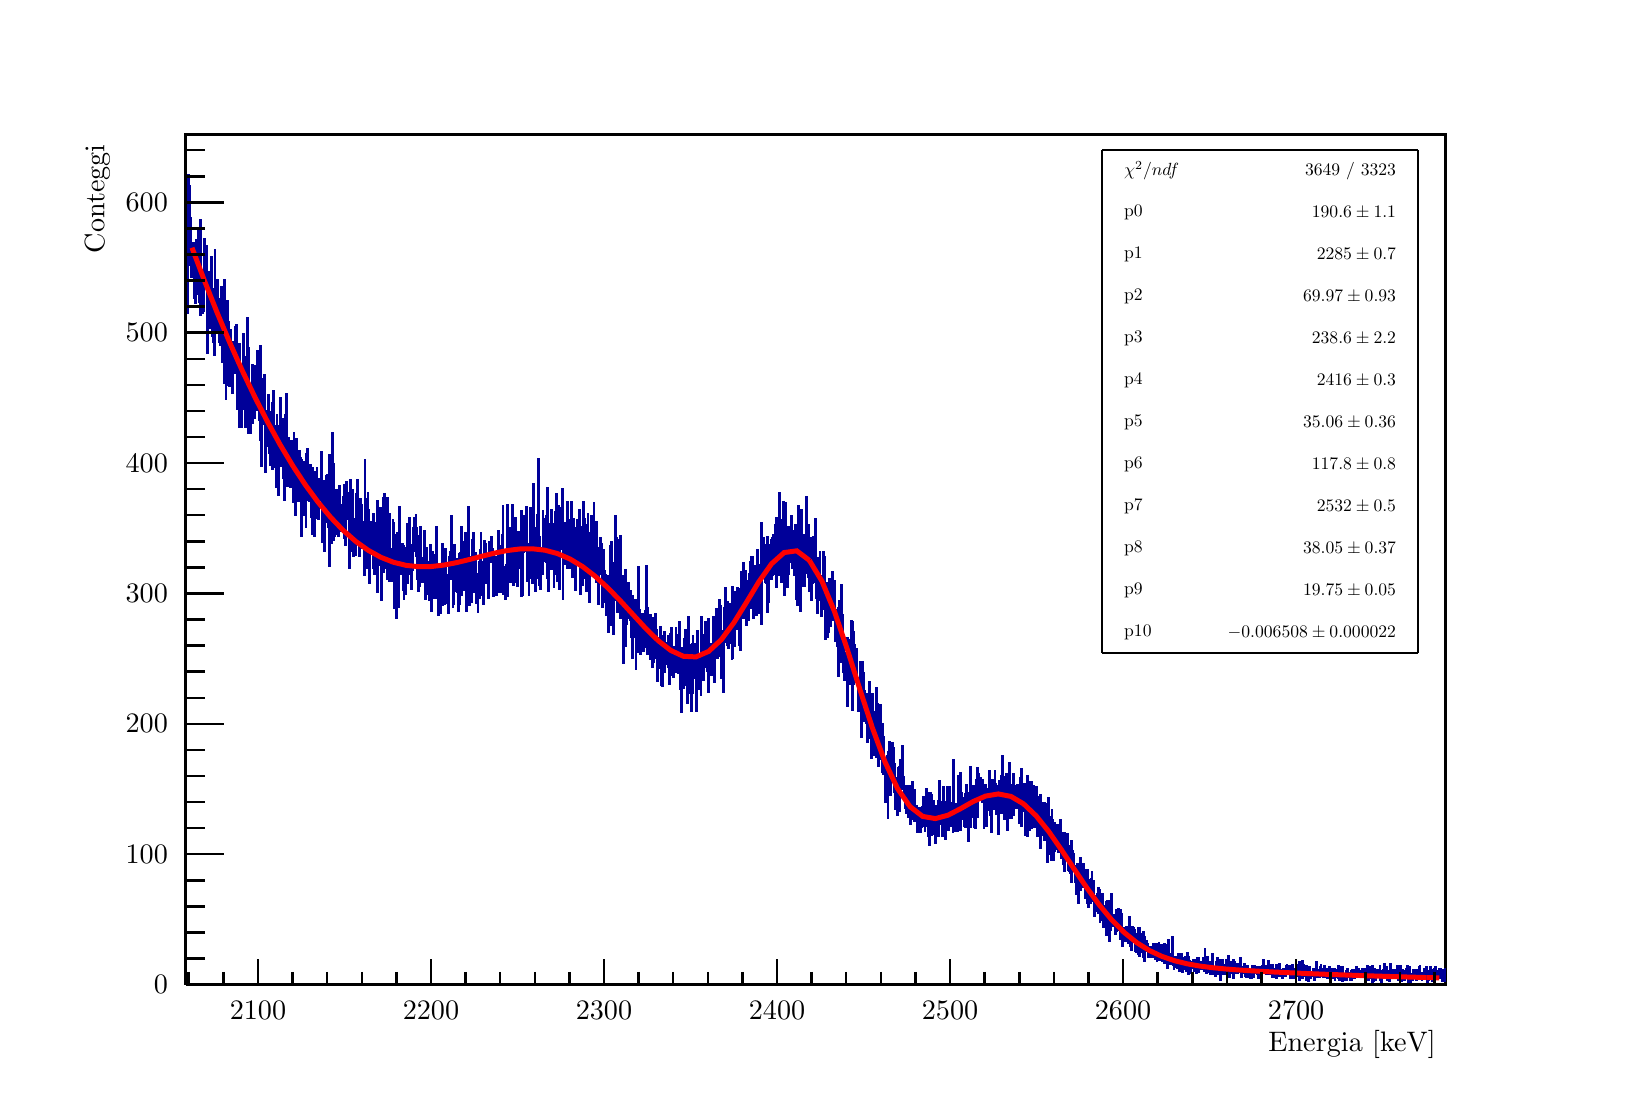
\begin{tikzpicture}
\pgfdeclareplotmark{cross} {
\pgfpathmoveto{\pgfpoint{-0.3\pgfplotmarksize}{\pgfplotmarksize}}
\pgfpathlineto{\pgfpoint{+0.3\pgfplotmarksize}{\pgfplotmarksize}}
\pgfpathlineto{\pgfpoint{+0.3\pgfplotmarksize}{0.3\pgfplotmarksize}}
\pgfpathlineto{\pgfpoint{+1\pgfplotmarksize}{0.3\pgfplotmarksize}}
\pgfpathlineto{\pgfpoint{+1\pgfplotmarksize}{-0.3\pgfplotmarksize}}
\pgfpathlineto{\pgfpoint{+0.3\pgfplotmarksize}{-0.3\pgfplotmarksize}}
\pgfpathlineto{\pgfpoint{+0.3\pgfplotmarksize}{-1.\pgfplotmarksize}}
\pgfpathlineto{\pgfpoint{-0.3\pgfplotmarksize}{-1.\pgfplotmarksize}}
\pgfpathlineto{\pgfpoint{-0.3\pgfplotmarksize}{-0.3\pgfplotmarksize}}
\pgfpathlineto{\pgfpoint{-1.\pgfplotmarksize}{-0.3\pgfplotmarksize}}
\pgfpathlineto{\pgfpoint{-1.\pgfplotmarksize}{0.3\pgfplotmarksize}}
\pgfpathlineto{\pgfpoint{-0.3\pgfplotmarksize}{0.3\pgfplotmarksize}}
\pgfpathclose
\pgfusepathqstroke
}
\pgfdeclareplotmark{cross*} {
\pgfpathmoveto{\pgfpoint{-0.3\pgfplotmarksize}{\pgfplotmarksize}}
\pgfpathlineto{\pgfpoint{+0.3\pgfplotmarksize}{\pgfplotmarksize}}
\pgfpathlineto{\pgfpoint{+0.3\pgfplotmarksize}{0.3\pgfplotmarksize}}
\pgfpathlineto{\pgfpoint{+1\pgfplotmarksize}{0.3\pgfplotmarksize}}
\pgfpathlineto{\pgfpoint{+1\pgfplotmarksize}{-0.3\pgfplotmarksize}}
\pgfpathlineto{\pgfpoint{+0.3\pgfplotmarksize}{-0.3\pgfplotmarksize}}
\pgfpathlineto{\pgfpoint{+0.3\pgfplotmarksize}{-1.\pgfplotmarksize}}
\pgfpathlineto{\pgfpoint{-0.3\pgfplotmarksize}{-1.\pgfplotmarksize}}
\pgfpathlineto{\pgfpoint{-0.3\pgfplotmarksize}{-0.3\pgfplotmarksize}}
\pgfpathlineto{\pgfpoint{-1.\pgfplotmarksize}{-0.3\pgfplotmarksize}}
\pgfpathlineto{\pgfpoint{-1.\pgfplotmarksize}{0.3\pgfplotmarksize}}
\pgfpathlineto{\pgfpoint{-0.3\pgfplotmarksize}{0.3\pgfplotmarksize}}
\pgfpathclose
\pgfusepathqfillstroke
}
\pgfdeclareplotmark{newstar} {
\pgfpathmoveto{\pgfqpoint{0pt}{\pgfplotmarksize}}
\pgfpathlineto{\pgfqpointpolar{44}{0.5\pgfplotmarksize}}
\pgfpathlineto{\pgfqpointpolar{18}{\pgfplotmarksize}}
\pgfpathlineto{\pgfqpointpolar{-20}{0.5\pgfplotmarksize}}
\pgfpathlineto{\pgfqpointpolar{-54}{\pgfplotmarksize}}
\pgfpathlineto{\pgfqpointpolar{-90}{0.5\pgfplotmarksize}}
\pgfpathlineto{\pgfqpointpolar{234}{\pgfplotmarksize}}
\pgfpathlineto{\pgfqpointpolar{198}{0.5\pgfplotmarksize}}
\pgfpathlineto{\pgfqpointpolar{162}{\pgfplotmarksize}}
\pgfpathlineto{\pgfqpointpolar{134}{0.5\pgfplotmarksize}}
\pgfpathclose
\pgfusepathqstroke
}
\pgfdeclareplotmark{newstar*} {
\pgfpathmoveto{\pgfqpoint{0pt}{\pgfplotmarksize}}
\pgfpathlineto{\pgfqpointpolar{44}{0.5\pgfplotmarksize}}
\pgfpathlineto{\pgfqpointpolar{18}{\pgfplotmarksize}}
\pgfpathlineto{\pgfqpointpolar{-20}{0.5\pgfplotmarksize}}
\pgfpathlineto{\pgfqpointpolar{-54}{\pgfplotmarksize}}
\pgfpathlineto{\pgfqpointpolar{-90}{0.5\pgfplotmarksize}}
\pgfpathlineto{\pgfqpointpolar{234}{\pgfplotmarksize}}
\pgfpathlineto{\pgfqpointpolar{198}{0.5\pgfplotmarksize}}
\pgfpathlineto{\pgfqpointpolar{162}{\pgfplotmarksize}}
\pgfpathlineto{\pgfqpointpolar{134}{0.5\pgfplotmarksize}}
\pgfpathclose
\pgfusepathqfillstroke
}
\definecolor{c}{rgb}{1,1,1};
\draw [color=c, fill=c] (0,0) rectangle (20,13.4957);
\draw [color=c, fill=c] (2,1.34957) rectangle (18,12.1461);
\definecolor{c}{rgb}{0,0,0};
\draw [c,line width=0.9] (2,1.34957) -- (2,12.1461) -- (18,12.1461) -- (18,1.34957) -- (2,1.34957);
\definecolor{c}{rgb}{1,1,1};
\draw [color=c, fill=c] (2,1.34957) rectangle (18,12.1461);
\definecolor{c}{rgb}{0,0,0};
\draw [c,line width=0.9] (2,1.34957) -- (2,12.1461) -- (18,12.1461) -- (18,1.34957) -- (2,1.34957);
\definecolor{c}{rgb}{0,0,0.6};
\draw [c,line width=0.9] (2,10.9366) -- (2.0048,10.9366) -- (2.0048,10.6717) -- (2.0096,10.6717) -- (2.0096,11.6155) -- (2.0144,11.6155) -- (2.0144,11.2181) -- (2.0192,11.2181) -- (2.0192,9.87687) -- (2.024,9.87687) -- (2.024,10.3405) --
 (2.02879,10.3405) -- (2.02879,10.8869) -- (2.03359,10.8869) -- (2.03359,11.632) -- (2.03839,11.632) -- (2.03839,10.4895) -- (2.04319,10.4895) -- (2.04319,10.4895) -- (2.04799,10.4895) -- (2.04799,11.483) -- (2.05279,11.483) -- (2.05279,11.4499) --
 (2.05759,11.4499) -- (2.05759,11.0856) -- (2.06239,11.0856) -- (2.06239,11.0028) -- (2.06719,11.0028) -- (2.06719,10.3405) -- (2.07199,10.3405) -- (2.07199,10.4895) -- (2.07678,10.4895) -- (2.07678,10.3405) -- (2.08158,10.3405) -- (2.08158,10.5226)
 -- (2.08638,10.5226) -- (2.08638,10.7544) -- (2.09118,10.7544) -- (2.09118,10.5226) -- (2.09598,10.5226) -- (2.09598,10.3571) -- (2.10078,10.3571) -- (2.10078,10.771) -- (2.10558,10.771) -- (2.10558,10.0756) -- (2.11038,10.0756) -- (2.11038,10.4895)
 -- (2.11518,10.4895) -- (2.11518,10.3902) -- (2.11998,10.3902) -- (2.11998,10.0093) -- (2.12478,10.0093) -- (2.12478,10.2246) -- (2.12957,10.2246) -- (2.12957,10.8041) -- (2.13437,10.8041) -- (2.13437,10.6882) -- (2.13917,10.6882) --
 (2.13917,10.4895) -- (2.14397,10.4895) -- (2.14397,10.1252) -- (2.14877,10.1252) -- (2.14877,10.7213) -- (2.15357,10.7213) -- (2.15357,10.92) -- (2.15837,10.92) -- (2.15837,10.1584) -- (2.16317,10.1584) -- (2.16317,10.7876) -- (2.16797,10.7876) --
 (2.16797,10.6717) -- (2.17277,10.6717) -- (2.17277,10.4233) -- (2.17756,10.4233) -- (2.17756,10.0259) -- (2.18236,10.0259) -- (2.18236,11.0525) -- (2.18716,11.0525) -- (2.18716,9.86032) -- (2.19196,9.86032) -- (2.19196,10.7048) -- (2.19676,10.7048)
 -- (2.19676,10.0093) -- (2.20156,10.0093) -- (2.20156,10.0093) -- (2.20636,10.0093) -- (2.20636,9.87687) -- (2.21116,9.87687) -- (2.21116,10.059) -- (2.21596,10.059) -- (2.21596,10.3074) -- (2.22076,10.3074) -- (2.22076,9.90999) -- (2.22556,9.90999)
 -- (2.22556,10.1749) -- (2.23035,10.1749) -- (2.23035,10.0921) -- (2.23515,10.0921) -- (2.23515,10.8207) -- (2.23995,10.8207) -- (2.23995,10.5889) -- (2.24475,10.5889) -- (2.24475,10.5889) -- (2.24955,10.5889) -- (2.24955,10.4233) --
 (2.25435,10.4233) -- (2.25435,10.2908) -- (2.25915,10.2908) -- (2.25915,10.3074) -- (2.26395,10.3074) -- (2.26395,10.7213) -- (2.26875,10.7213) -- (2.26875,10.0093) -- (2.27355,10.0093) -- (2.27355,9.38014) -- (2.27834,9.38014) -- (2.27834,10.059)
 -- (2.28314,10.059) -- (2.28314,10.3902) -- (2.28794,10.3902) -- (2.28794,9.92655) -- (2.29274,9.92655) -- (2.29274,10.3571) -- (2.29754,10.3571) -- (2.29754,9.81064) -- (2.30234,9.81064) -- (2.30234,9.74441) -- (2.30714,9.74441) --
 (2.30714,9.69474) -- (2.31194,9.69474) -- (2.31194,10.2246) -- (2.31674,10.2246) -- (2.31674,9.90999) -- (2.32154,9.90999) -- (2.32154,10.5889) -- (2.32633,10.5889) -- (2.32633,10.059) -- (2.33113,10.059) -- (2.33113,10.473) -- (2.33593,10.473) --
 (2.33593,9.59539) -- (2.34073,9.59539) -- (2.34073,9.86032) -- (2.34553,9.86032) -- (2.34553,10.1749) -- (2.35033,10.1749) -- (2.35033,9.5126) -- (2.35513,9.5126) -- (2.35513,9.87687) -- (2.35993,9.87687) -- (2.35993,10.1087) -- (2.36473,10.1087) --
 (2.36473,9.34702) -- (2.36953,9.34702) -- (2.36953,10.6717) -- (2.37433,10.6717) -- (2.37433,10.1749) -- (2.37912,10.1749) -- (2.37912,10.1584) -- (2.38392,10.1584) -- (2.38392,9.62851) -- (2.38872,9.62851) -- (2.38872,9.92655) -- (2.39352,9.92655)
 -- (2.39352,9.62851) -- (2.39832,9.62851) -- (2.39832,9.84376) -- (2.40312,9.84376) -- (2.40312,10.2908) -- (2.40792,10.2908) -- (2.40792,10.0093) -- (2.41272,10.0093) -- (2.41272,10.059) -- (2.41752,10.059) -- (2.41752,9.64506) -- (2.42232,9.64506)
 -- (2.42232,9.99278) -- (2.42711,9.99278) -- (2.42711,9.5126) -- (2.43191,9.5126) -- (2.43191,9.94311) -- (2.43671,9.94311) -- (2.43671,9.76097) -- (2.44151,9.76097) -- (2.44151,9.47949) -- (2.44631,9.47949) -- (2.44631,10.0093) -- (2.45111,10.0093)
 -- (2.45111,9.61195) -- (2.45591,9.61195) -- (2.45591,10.208) -- (2.46071,10.208) -- (2.46071,9.26423) -- (2.46551,9.26423) -- (2.46551,9.47949) -- (2.47031,9.47949) -- (2.47031,9.90999) -- (2.47511,9.90999) -- (2.47511,9.81064) -- (2.4799,9.81064)
 -- (2.4799,9.41325) -- (2.4847,9.41325) -- (2.4847,8.99931) -- (2.4895,8.99931) -- (2.4895,9.09865) -- (2.4943,9.09865) -- (2.4943,10.2908) -- (2.4991,10.2908) -- (2.4991,9.7113) -- (2.5039,9.7113) -- (2.5039,9.56227) -- (2.5087,9.56227) --
 (2.5087,8.78406) -- (2.5135,8.78406) -- (2.5135,9.09865) -- (2.5183,9.09865) -- (2.5183,9.11521) -- (2.5231,9.11521) -- (2.5231,8.96619) -- (2.52789,8.96619) -- (2.52789,10.0259) -- (2.53269,10.0259) -- (2.53269,9.18144) -- (2.53749,9.18144) --
 (2.53749,9.61195) -- (2.54229,9.61195) -- (2.54229,9.56227) -- (2.54709,9.56227) -- (2.54709,9.76097) -- (2.55189,9.76097) -- (2.55189,9.28079) -- (2.55669,9.28079) -- (2.55669,8.94963) -- (2.56149,8.94963) -- (2.56149,9.66162) -- (2.56629,9.66162)
 -- (2.56629,9.47949) -- (2.57109,9.47949) -- (2.57109,8.99931) -- (2.57589,8.99931) -- (2.57589,9.31391) -- (2.58068,9.31391) -- (2.58068,9.42981) -- (2.58548,9.42981) -- (2.58548,8.96619) -- (2.59028,8.96619) -- (2.59028,9.38014) --
 (2.59508,9.38014) -- (2.59508,8.86685) -- (2.59988,8.86685) -- (2.59988,9.5126) -- (2.60468,9.5126) -- (2.60468,9.33047) -- (2.60948,9.33047) -- (2.60948,9.28079) -- (2.61428,9.28079) -- (2.61428,9.11521) -- (2.61908,9.11521) -- (2.61908,9.42981) --
 (2.62388,9.42981) -- (2.62388,9.24768) -- (2.62867,9.24768) -- (2.62867,9.38014) -- (2.63347,9.38014) -- (2.63347,9.69474) -- (2.63827,9.69474) -- (2.63827,9.72785) -- (2.64307,9.72785) -- (2.64307,9.41325) -- (2.64787,9.41325) -- (2.64787,9.66162)
 -- (2.65267,9.66162) -- (2.65267,8.66815) -- (2.65747,8.66815) -- (2.65747,8.81717) -- (2.66227,8.81717) -- (2.66227,9.16489) -- (2.66707,9.16489) -- (2.66707,8.73438) -- (2.67187,8.73438) -- (2.67187,9.24768) -- (2.67666,9.24768) --
 (2.67666,9.47949) -- (2.68146,9.47949) -- (2.68146,8.43634) -- (2.68626,8.43634) -- (2.68626,9.11521) -- (2.69106,9.11521) -- (2.69106,8.8834) -- (2.69586,8.8834) -- (2.69586,9.11521) -- (2.70066,9.11521) -- (2.70066,8.96619) -- (2.70546,8.96619) --
 (2.70546,8.43634) -- (2.71026,8.43634) -- (2.71026,9.01587) -- (2.71506,9.01587) -- (2.71506,8.96619) -- (2.71986,8.96619) -- (2.71986,9.09865) -- (2.72466,9.09865) -- (2.72466,9.04898) -- (2.72945,9.04898) -- (2.72945,9.61195) -- (2.73425,9.61195)
 -- (2.73425,8.99931) -- (2.73905,8.99931) -- (2.73905,9.16489) -- (2.74385,9.16489) -- (2.74385,8.66815) -- (2.74865,8.66815) -- (2.74865,8.98275) -- (2.75345,8.98275) -- (2.75345,8.43634) -- (2.75825,8.43634) -- (2.75825,9.01587) --
 (2.76305,9.01587) -- (2.76305,8.86685) -- (2.76785,8.86685) -- (2.76785,9.31391) -- (2.77265,9.31391) -- (2.77265,9.16489) -- (2.77744,9.16489) -- (2.77744,8.68471) -- (2.78224,8.68471) -- (2.78224,9.81064) -- (2.78704,9.81064) -- (2.78704,8.63503)
 -- (2.79184,8.63503) -- (2.79184,8.93308) -- (2.79664,8.93308) -- (2.79664,8.35355) -- (2.80144,8.35355) -- (2.80144,9.42981) -- (2.80624,9.42981) -- (2.80624,8.50257) -- (2.81104,8.50257) -- (2.81104,8.8834) -- (2.81584,8.8834) -- (2.81584,8.75094)
 -- (2.82064,8.75094) -- (2.82064,8.71782) -- (2.82544,8.71782) -- (2.82544,8.35355) -- (2.83023,8.35355) -- (2.83023,8.8834) -- (2.83503,8.8834) -- (2.83503,8.86685) -- (2.83983,8.86685) -- (2.83983,8.99931) -- (2.84463,8.99931) -- (2.84463,9.21456)
 -- (2.84943,9.21456) -- (2.84943,8.48601) -- (2.85423,8.48601) -- (2.85423,8.99931) -- (2.85903,8.99931) -- (2.85903,8.99931) -- (2.86383,8.99931) -- (2.86383,8.93308) -- (2.86863,8.93308) -- (2.86863,8.83373) -- (2.87343,8.83373) -- (2.87343,9.198)
 -- (2.87822,9.198) -- (2.87822,8.55225) -- (2.88302,8.55225) -- (2.88302,9.09865) -- (2.88782,9.09865) -- (2.88782,8.68471) -- (2.89262,8.68471) -- (2.89262,8.73438) -- (2.89742,8.73438) -- (2.89742,9.13177) -- (2.90222,9.13177) -- (2.90222,9.04898)
 -- (2.90702,9.04898) -- (2.90702,8.65159) -- (2.91182,8.65159) -- (2.91182,9.3967) -- (2.91662,9.3967) -- (2.91662,8.68471) -- (2.92142,8.68471) -- (2.92142,8.73438) -- (2.92621,8.73438) -- (2.92621,8.89996) -- (2.93101,8.89996) -- (2.93101,8.51913)
 -- (2.93581,8.51913) -- (2.93581,8.58536) -- (2.94061,8.58536) -- (2.94061,8.27076) -- (2.94541,8.27076) -- (2.94541,9.0821) -- (2.95021,9.0821) -- (2.95021,9.46293) -- (2.95501,9.46293) -- (2.95501,8.33699) -- (2.95981,8.33699) -- (2.95981,7.9396)
 -- (2.96461,7.9396) -- (2.96461,8.63503) -- (2.96941,8.63503) -- (2.96941,9.01587) -- (2.97421,9.01587) -- (2.97421,8.63503) -- (2.979,8.63503) -- (2.979,8.55225) -- (2.9838,8.55225) -- (2.9838,9.03242) -- (2.9886,9.03242) -- (2.9886,8.46946) --
 (2.9934,8.46946) -- (2.9934,8.65159) -- (2.9982,8.65159) -- (2.9982,8.75094) -- (3.003,8.75094) -- (3.003,9.0821) -- (3.0078,9.0821) -- (3.0078,7.85681) -- (3.0126,7.85681) -- (3.0126,8.27076) -- (3.0174,8.27076) -- (3.0174,8.4529) --
 (3.0222,8.4529) -- (3.0222,8.63503) -- (3.02699,8.63503) -- (3.02699,8.18797) -- (3.03179,8.18797) -- (3.03179,8.37011) -- (3.03659,8.37011) -- (3.03659,8.48601) -- (3.04139,8.48601) -- (3.04139,8.55225) -- (3.04619,8.55225) -- (3.04619,8.83373) --
 (3.05099,8.83373) -- (3.05099,8.4529) -- (3.05579,8.4529) -- (3.05579,8.4529) -- (3.06059,8.4529) -- (3.06059,8.40322) -- (3.06539,8.40322) -- (3.06539,8.10518) -- (3.07019,8.10518) -- (3.07019,8.41978) -- (3.07499,8.41978) -- (3.07499,7.95616) --
 (3.07978,7.95616) -- (3.07978,8.27076) -- (3.08458,8.27076) -- (3.08458,8.61848) -- (3.08938,8.61848) -- (3.08938,8.22109) -- (3.09418,8.22109) -- (3.09418,8.48601) -- (3.09898,8.48601) -- (3.09898,8.73438) -- (3.10378,8.73438) -- (3.10378,7.90649)
 -- (3.10858,7.90649) -- (3.10858,8.17141) -- (3.11338,8.17141) -- (3.11338,8.8834) -- (3.11818,8.8834) -- (3.11818,8.53569) -- (3.12298,8.53569) -- (3.12298,8.43634) -- (3.12777,8.43634) -- (3.12777,8.41978) -- (3.13257,8.41978) -- (3.13257,8.40322)
 -- (3.13737,8.40322) -- (3.13737,8.17141) -- (3.14217,8.17141) -- (3.14217,7.92305) -- (3.14697,7.92305) -- (3.14697,8.02239) -- (3.15177,8.02239) -- (3.15177,7.67468) -- (3.15657,7.67468) -- (3.15657,8.58536) -- (3.16137,8.58536) --
 (3.16137,8.02239) -- (3.16617,8.02239) -- (3.16617,7.84026) -- (3.17097,7.84026) -- (3.17097,7.57533) -- (3.17577,7.57533) -- (3.17577,8.10518) -- (3.18056,8.10518) -- (3.18056,8.43634) -- (3.18536,8.43634) -- (3.18536,8.17141) -- (3.19016,8.17141)
 -- (3.19016,8.2542) -- (3.19496,8.2542) -- (3.19496,7.9396) -- (3.19976,7.9396) -- (3.19976,7.9396) -- (3.20456,7.9396) -- (3.20456,8.80061) -- (3.20936,8.80061) -- (3.20936,8.15486) -- (3.21416,8.15486) -- (3.21416,8.43634) -- (3.21896,8.43634) --
 (3.21896,8.38667) -- (3.22376,8.38667) -- (3.22376,8.28732) -- (3.22855,8.28732) -- (3.22855,8.53569) -- (3.23335,8.53569) -- (3.23335,8.40322) -- (3.23815,8.40322) -- (3.23815,7.85681) -- (3.24295,7.85681) -- (3.24295,7.79058) -- (3.24775,7.79058)
 -- (3.24775,8.15486) -- (3.25255,8.15486) -- (3.25255,7.5091) -- (3.25735,7.5091) -- (3.25735,8.32043) -- (3.26215,8.32043) -- (3.26215,8.58536) -- (3.26695,8.58536) -- (3.26695,8.08862) -- (3.27175,8.08862) -- (3.27175,8.48601) -- (3.27654,8.48601)
 -- (3.27654,7.80714) -- (3.28134,7.80714) -- (3.28134,8.85029) -- (3.28614,8.85029) -- (3.28614,7.69124) -- (3.29094,7.69124) -- (3.29094,8.1383) -- (3.29574,8.1383) -- (3.29574,7.87337) -- (3.30054,7.87337) -- (3.30054,8.07207) -- (3.30534,8.07207)
 -- (3.30534,8.28732) -- (3.31014,8.28732) -- (3.31014,8.05551) -- (3.31494,8.05551) -- (3.31494,8.10518) -- (3.31974,8.10518) -- (3.31974,8.05551) -- (3.32454,8.05551) -- (3.32454,7.90649) -- (3.32933,7.90649) -- (3.32933,7.67468) --
 (3.33413,7.67468) -- (3.33413,7.80714) -- (3.33893,7.80714) -- (3.33893,7.85681) -- (3.34373,7.85681) -- (3.34373,8.2542) -- (3.34853,8.2542) -- (3.34853,8.15486) -- (3.35333,8.15486) -- (3.35333,8.22109) -- (3.35813,8.22109) -- (3.35813,8.00584) --
 (3.36293,8.00584) -- (3.36293,7.95616) -- (3.36773,7.95616) -- (3.36773,7.47598) -- (3.37253,7.47598) -- (3.37253,8.35355) -- (3.37732,8.35355) -- (3.37732,8.12174) -- (3.38212,8.12174) -- (3.38212,7.95616) -- (3.38692,7.95616) -- (3.38692,7.3104)
 -- (3.39172,7.3104) -- (3.39172,8.18797) -- (3.39652,8.18797) -- (3.39652,8.27076) -- (3.40132,8.27076) -- (3.40132,8.27076) -- (3.40612,8.27076) -- (3.40612,7.84026) -- (3.41092,7.84026) -- (3.41092,7.59189) -- (3.41572,7.59189) --
 (3.41572,7.55877) -- (3.42052,7.55877) -- (3.42052,7.64156) -- (3.42532,7.64156) -- (3.42532,7.98928) -- (3.43011,7.98928) -- (3.43011,7.49254) -- (3.43491,7.49254) -- (3.43491,7.57533) -- (3.43971,7.57533) -- (3.43971,7.70779) -- (3.44451,7.70779)
 -- (3.44451,8.12174) -- (3.44931,8.12174) -- (3.44931,7.84026) -- (3.45411,7.84026) -- (3.45411,8.03895) -- (3.45891,8.03895) -- (3.45891,7.60845) -- (3.46371,7.60845) -- (3.46371,8.00584) -- (3.46851,8.00584) -- (3.46851,7.04548) --
 (3.47331,7.04548) -- (3.47331,7.44287) -- (3.4781,7.44287) -- (3.4781,7.44287) -- (3.4829,7.44287) -- (3.4829,7.52566) -- (3.4877,7.52566) -- (3.4877,7.70779) -- (3.4925,7.70779) -- (3.4925,7.98928) -- (3.4973,7.98928) -- (3.4973,7.87337) --
 (3.5021,7.87337) -- (3.5021,7.45943) -- (3.5069,7.45943) -- (3.5069,7.69124) -- (3.5117,7.69124) -- (3.5117,7.3104) -- (3.5165,7.3104) -- (3.5165,7.70779) -- (3.5213,7.70779) -- (3.5213,7.42631) -- (3.52609,7.42631) -- (3.52609,7.16138) --
 (3.53089,7.16138) -- (3.53089,8.08862) -- (3.53569,8.08862) -- (3.53569,7.75747) -- (3.54049,7.75747) -- (3.54049,8.15486) -- (3.54529,8.15486) -- (3.54529,7.95616) -- (3.55009,7.95616) -- (3.55009,7.80714) -- (3.55489,7.80714) -- (3.55489,7.74091)
 -- (3.55969,7.74091) -- (3.55969,7.5091) -- (3.56449,7.5091) -- (3.56449,7.92305) -- (3.56929,7.92305) -- (3.56929,7.55877) -- (3.57409,7.55877) -- (3.57409,7.49254) -- (3.57888,7.49254) -- (3.57888,7.75747) -- (3.58368,7.75747) -- (3.58368,7.9396)
 -- (3.58848,7.9396) -- (3.58848,7.29385) -- (3.59328,7.29385) -- (3.59328,7.52566) -- (3.59808,7.52566) -- (3.59808,7.55877) -- (3.60288,7.55877) -- (3.60288,7.44287) -- (3.60768,7.44287) -- (3.60768,7.90649) -- (3.61248,7.90649) --
 (3.61248,7.07859) -- (3.61728,7.07859) -- (3.61728,7.72435) -- (3.62208,7.72435) -- (3.62208,7.8237) -- (3.62687,7.8237) -- (3.62687,7.59189) -- (3.63167,7.59189) -- (3.63167,7.67468) -- (3.63647,7.67468) -- (3.63647,7.04548) -- (3.64127,7.04548) --
 (3.64127,7.85681) -- (3.64607,7.85681) -- (3.64607,7.5091) -- (3.65087,7.5091) -- (3.65087,7.27729) -- (3.65567,7.27729) -- (3.65567,7.65812) -- (3.66047,7.65812) -- (3.66047,7.3104) -- (3.66527,7.3104) -- (3.66527,7.90649) -- (3.67007,7.90649) --
 (3.67007,7.40975) -- (3.67487,7.40975) -- (3.67487,7.45943) -- (3.67966,7.45943) -- (3.67966,7.40975) -- (3.68446,7.40975) -- (3.68446,7.75747) -- (3.68926,7.75747) -- (3.68926,7.26073) -- (3.69406,7.26073) -- (3.69406,7.77402) -- (3.69886,7.77402)
 -- (3.69886,7.70779) -- (3.70366,7.70779) -- (3.70366,7.52566) -- (3.70846,7.52566) -- (3.70846,7.67468) -- (3.71326,7.67468) -- (3.71326,7.65812) -- (3.71806,7.65812) -- (3.71806,8.10518) -- (3.72286,8.10518) -- (3.72286,7.5091) -- (3.72765,7.5091)
 -- (3.72765,7.55877) -- (3.73245,7.55877) -- (3.73245,6.97925) -- (3.73725,6.97925) -- (3.73725,7.14483) -- (3.74205,7.14483) -- (3.74205,7.40975) -- (3.74685,7.40975) -- (3.74685,7.74091) -- (3.75165,7.74091) -- (3.75165,7.40975) --
 (3.75645,7.40975) -- (3.75645,6.86334) -- (3.76125,6.86334) -- (3.76125,7.29385) -- (3.76605,7.29385) -- (3.76605,7.74091) -- (3.77085,7.74091) -- (3.77085,7.52566) -- (3.77565,7.52566) -- (3.77565,7.22762) -- (3.78044,7.22762) -- (3.78044,7.59189)
 -- (3.78524,7.59189) -- (3.78524,7.80714) -- (3.79004,7.80714) -- (3.79004,7.45943) -- (3.79484,7.45943) -- (3.79484,7.8237) -- (3.79964,7.8237) -- (3.79964,7.52566) -- (3.80444,7.52566) -- (3.80444,7.67468) -- (3.80924,7.67468) -- (3.80924,7.16138)
 -- (3.81404,7.16138) -- (3.81404,7.8237) -- (3.81884,7.8237) -- (3.81884,6.66465) -- (3.82364,6.66465) -- (3.82364,7.42631) -- (3.82843,7.42631) -- (3.82843,8.07207) -- (3.83323,8.07207) -- (3.83323,7.625) -- (3.83803,7.625) -- (3.83803,7.27729) --
 (3.84283,7.27729) -- (3.84283,7.39319) -- (3.84763,7.39319) -- (3.84763,7.55877) -- (3.85243,7.55877) -- (3.85243,6.96269) -- (3.85723,6.96269) -- (3.85723,7.59189) -- (3.86203,7.59189) -- (3.86203,7.29385) -- (3.86683,7.29385) -- (3.86683,8.35355)
 -- (3.87163,8.35355) -- (3.87163,6.99581) -- (3.87642,6.99581) -- (3.87642,7.95616) -- (3.88122,7.95616) -- (3.88122,7.49254) -- (3.88602,7.49254) -- (3.88602,7.04548) -- (3.89082,7.04548) -- (3.89082,7.27729) -- (3.89562,7.27729) --
 (3.89562,7.36008) -- (3.90042,7.36008) -- (3.90042,7.21106) -- (3.90522,7.21106) -- (3.90522,7.07859) -- (3.91002,7.07859) -- (3.91002,7.625) -- (3.91482,7.625) -- (3.91482,7.54221) -- (3.91962,7.54221) -- (3.91962,7.5091) -- (3.92442,7.5091) --
 (3.92442,7.32696) -- (3.92921,7.32696) -- (3.92921,7.39319) -- (3.93401,7.39319) -- (3.93401,7.04548) -- (3.93881,7.04548) -- (3.93881,7.24417) -- (3.94361,7.24417) -- (3.94361,7.34352) -- (3.94841,7.34352) -- (3.94841,7.45943) -- (3.95321,7.45943)
 -- (3.95321,7.67468) -- (3.95801,7.67468) -- (3.95801,7.40975) -- (3.96281,7.40975) -- (3.96281,7.44287) -- (3.96761,7.44287) -- (3.96761,7.42631) -- (3.97241,7.42631) -- (3.97241,7.42631) -- (3.9772,7.42631) -- (3.9772,7.11171) -- (3.982,7.11171)
 -- (3.982,7.39319) -- (3.9868,7.39319) -- (3.9868,7.14483) -- (3.9916,7.14483) -- (3.9916,7.3104) -- (3.9964,7.3104) -- (3.9964,7.24417) -- (4.0012,7.24417) -- (4.0012,7.1945) -- (4.006,7.1945) -- (4.006,7.54221) -- (4.0108,7.54221) --
 (4.0108,7.02892) -- (4.0156,7.02892) -- (4.0156,7.69124) -- (4.0204,7.69124) -- (4.0204,7.625) -- (4.0252,7.625) -- (4.0252,7.14483) -- (4.02999,7.14483) -- (4.02999,6.92957) -- (4.03479,6.92957) -- (4.03479,7.26073) -- (4.03959,7.26073) --
 (4.03959,7.69124) -- (4.04439,7.69124) -- (4.04439,7.72435) -- (4.04919,7.72435) -- (4.04919,7.40975) -- (4.05399,7.40975) -- (4.05399,7.37664) -- (4.05879,7.37664) -- (4.05879,7.47598) -- (4.06359,7.47598) -- (4.06359,7.44287) -- (4.06839,7.44287)
 -- (4.06839,7.47598) -- (4.07319,7.47598) -- (4.07319,7.17794) -- (4.07798,7.17794) -- (4.07798,7.59189) -- (4.08278,7.59189) -- (4.08278,6.64809) -- (4.08758,6.64809) -- (4.08758,7.70779) -- (4.09238,7.70779) -- (4.09238,7.75747) --
 (4.09718,7.75747) -- (4.09718,7.21106) -- (4.10198,7.21106) -- (4.10198,7.42631) -- (4.10678,7.42631) -- (4.10678,6.86334) -- (4.11158,6.86334) -- (4.11158,6.94613) -- (4.11638,6.94613) -- (4.11638,7.625) -- (4.12118,7.625) -- (4.12118,7.36008) --
 (4.12598,7.36008) -- (4.12598,7.11171) -- (4.13077,7.11171) -- (4.13077,6.79711) -- (4.13557,6.79711) -- (4.13557,6.8799) -- (4.14037,6.8799) -- (4.14037,6.92957) -- (4.14517,6.92957) -- (4.14517,7.12827) -- (4.14997,7.12827) -- (4.14997,7.26073) --
 (4.15477,7.26073) -- (4.15477,6.81367) -- (4.15957,6.81367) -- (4.15957,6.84678) -- (4.16437,6.84678) -- (4.16437,7.39319) -- (4.16917,7.39319) -- (4.16917,7.57533) -- (4.17397,7.57533) -- (4.17397,7.16138) -- (4.17876,7.16138) -- (4.17876,7.34352)
 -- (4.18356,7.34352) -- (4.18356,7.75747) -- (4.18836,7.75747) -- (4.18836,7.39319) -- (4.19316,7.39319) -- (4.19316,6.99581) -- (4.19796,6.99581) -- (4.19796,6.96269) -- (4.20276,6.96269) -- (4.20276,6.79711) -- (4.20756,6.79711) --
 (4.20756,7.37664) -- (4.21236,7.37664) -- (4.21236,7.5091) -- (4.21716,7.5091) -- (4.21716,7.27729) -- (4.22196,7.27729) -- (4.22196,7.26073) -- (4.22675,7.26073) -- (4.22675,7.09515) -- (4.23155,7.09515) -- (4.23155,7.06204) -- (4.23635,7.06204) --
 (4.23635,7.44287) -- (4.24115,7.44287) -- (4.24115,6.89646) -- (4.24595,6.89646) -- (4.24595,7.16138) -- (4.25075,7.16138) -- (4.25075,7.22762) -- (4.25555,7.22762) -- (4.25555,7.11171) -- (4.26035,7.11171) -- (4.26035,6.91302) -- (4.26515,6.91302)
 -- (4.26515,6.54874) -- (4.26995,6.54874) -- (4.26995,7.11171) -- (4.27474,7.11171) -- (4.27474,8.00584) -- (4.27954,8.00584) -- (4.27954,6.8799) -- (4.28434,6.8799) -- (4.28434,7.22762) -- (4.28914,7.22762) -- (4.28914,6.64809) -- (4.29394,6.64809)
 -- (4.29394,6.8799) -- (4.29874,6.8799) -- (4.29874,6.81367) -- (4.30354,6.81367) -- (4.30354,6.89646) -- (4.30834,6.89646) -- (4.30834,7.5091) -- (4.31314,7.5091) -- (4.31314,7.59189) -- (4.31794,7.59189) -- (4.31794,7.37664) -- (4.32274,7.37664)
 -- (4.32274,7.07859) -- (4.32753,7.07859) -- (4.32753,6.4494) -- (4.33233,6.4494) -- (4.33233,7.01236) -- (4.33713,7.01236) -- (4.33713,6.51563) -- (4.34193,6.51563) -- (4.34193,6.8799) -- (4.34673,6.8799) -- (4.34673,6.83023) -- (4.35153,6.83023)
 -- (4.35153,6.99581) -- (4.35633,6.99581) -- (4.35633,6.92957) -- (4.36113,6.92957) -- (4.36113,7.22762) -- (4.36593,7.22762) -- (4.36593,6.89646) -- (4.37073,6.89646) -- (4.37073,6.97925) -- (4.37552,6.97925) -- (4.37552,6.69776) --
 (4.38032,6.69776) -- (4.38032,6.64809) -- (4.38512,6.64809) -- (4.38512,7.32696) -- (4.38992,7.32696) -- (4.38992,7.06204) -- (4.39472,7.06204) -- (4.39472,6.5653) -- (4.39952,6.5653) -- (4.39952,6.96269) -- (4.40432,6.96269) -- (4.40432,7.21106) --
 (4.40912,7.21106) -- (4.40912,6.8799) -- (4.41392,6.8799) -- (4.41392,6.63153) -- (4.41872,6.63153) -- (4.41872,7.16138) -- (4.42352,7.16138) -- (4.42352,6.73088) -- (4.42831,6.73088) -- (4.42831,7.49254) -- (4.43311,7.49254) -- (4.43311,7.07859) --
 (4.43791,7.07859) -- (4.43791,6.33349) -- (4.44271,6.33349) -- (4.44271,6.74744) -- (4.44751,6.74744) -- (4.44751,7.22762) -- (4.45231,7.22762) -- (4.45231,7.22762) -- (4.45711,7.22762) -- (4.45711,6.68121) -- (4.46191,6.68121) -- (4.46191,7.21106)
 -- (4.46671,7.21106) -- (4.46671,7.39319) -- (4.47151,7.39319) -- (4.47151,6.81367) -- (4.47631,6.81367) -- (4.47631,7.22762) -- (4.4811,7.22762) -- (4.4811,7.02892) -- (4.4859,7.02892) -- (4.4859,6.23414) -- (4.4907,6.23414) -- (4.4907,6.59842) --
 (4.4955,6.59842) -- (4.4955,6.96269) -- (4.5003,6.96269) -- (4.5003,7.16138) -- (4.5051,7.16138) -- (4.5051,7.16138) -- (4.5099,7.16138) -- (4.5099,6.59842) -- (4.5147,6.59842) -- (4.5147,7.52566) -- (4.5195,7.52566) -- (4.5195,7.57533) --
 (4.5243,7.57533) -- (4.5243,6.64809) -- (4.52909,6.64809) -- (4.52909,6.86334) -- (4.53389,6.86334) -- (4.53389,7.47598) -- (4.53869,7.47598) -- (4.53869,6.66465) -- (4.54349,6.66465) -- (4.54349,7.11171) -- (4.54829,7.11171) -- (4.54829,6.96269) --
 (4.55309,6.96269) -- (4.55309,6.92957) -- (4.55789,6.92957) -- (4.55789,7.52566) -- (4.56269,7.52566) -- (4.56269,6.49907) -- (4.56749,6.49907) -- (4.56749,6.83023) -- (4.57229,6.83023) -- (4.57229,6.74744) -- (4.57708,6.74744) -- (4.57708,6.84678)
 -- (4.58188,6.84678) -- (4.58188,6.48251) -- (4.58668,6.48251) -- (4.58668,7.32696) -- (4.59148,7.32696) -- (4.59148,6.8799) -- (4.59628,6.8799) -- (4.59628,6.8799) -- (4.60108,6.8799) -- (4.60108,6.5653) -- (4.60588,6.5653) -- (4.60588,6.48251) --
 (4.61068,6.48251) -- (4.61068,6.81367) -- (4.61548,6.81367) -- (4.61548,6.64809) -- (4.62028,6.64809) -- (4.62028,6.66465) -- (4.62508,6.66465) -- (4.62508,6.71432) -- (4.62987,6.71432) -- (4.62987,7.24417) -- (4.63467,7.24417) -- (4.63467,7.02892)
 -- (4.63947,7.02892) -- (4.63947,7.21106) -- (4.64427,7.21106) -- (4.64427,6.1348) -- (4.64907,6.1348) -- (4.64907,6.78055) -- (4.65387,6.78055) -- (4.65387,6.89646) -- (4.65867,6.89646) -- (4.65867,6.89646) -- (4.66347,6.89646) -- (4.66347,7.06204)
 -- (4.66827,7.06204) -- (4.66827,6.58186) -- (4.67307,6.58186) -- (4.67307,6.00233) -- (4.67786,6.00233) -- (4.67786,7.02892) -- (4.68266,7.02892) -- (4.68266,7.07859) -- (4.68746,7.07859) -- (4.68746,6.64809) -- (4.69226,6.64809) --
 (4.69226,6.99581) -- (4.69706,6.99581) -- (4.69706,6.8799) -- (4.70186,6.8799) -- (4.70186,6.15135) -- (4.70666,6.15135) -- (4.70666,7.16138) -- (4.71146,7.16138) -- (4.71146,6.69776) -- (4.71626,6.69776) -- (4.71626,7.40975) -- (4.72106,7.40975) --
 (4.72106,6.81367) -- (4.72585,6.81367) -- (4.72585,6.66465) -- (4.73065,6.66465) -- (4.73065,6.5653) -- (4.73545,6.5653) -- (4.73545,6.71432) -- (4.74025,6.71432) -- (4.74025,6.71432) -- (4.74505,6.71432) -- (4.74505,6.64809) -- (4.74985,6.64809) --
 (4.74985,6.94613) -- (4.75465,6.94613) -- (4.75465,6.76399) -- (4.75945,6.76399) -- (4.75945,6.36661) -- (4.76425,6.36661) -- (4.76425,6.91302) -- (4.76905,6.91302) -- (4.76905,6.2507) -- (4.77385,6.2507) -- (4.77385,6.86334) -- (4.77864,6.86334) --
 (4.77864,6.71432) -- (4.78344,6.71432) -- (4.78344,6.31693) -- (4.78824,6.31693) -- (4.78824,6.66465) -- (4.79304,6.66465) -- (4.79304,6.74744) -- (4.79784,6.74744) -- (4.79784,6.61497) -- (4.80264,6.61497) -- (4.80264,6.89646) -- (4.80744,6.89646)
 -- (4.80744,6.69776) -- (4.81224,6.69776) -- (4.81224,6.4494) -- (4.81704,6.4494) -- (4.81704,7.1945) -- (4.82184,7.1945) -- (4.82184,6.8799) -- (4.82663,6.8799) -- (4.82663,6.97925) -- (4.83143,6.97925) -- (4.83143,7.01236) -- (4.83623,7.01236) --
 (4.83623,7.27729) -- (4.84103,7.27729) -- (4.84103,6.5653) -- (4.84583,6.5653) -- (4.84583,7.04548) -- (4.85063,7.04548) -- (4.85063,6.66465) -- (4.85543,6.66465) -- (4.85543,6.74744) -- (4.86023,6.74744) -- (4.86023,6.84678) -- (4.86503,6.84678) --
 (4.86503,6.38316) -- (4.86983,6.38316) -- (4.86983,6.41628) -- (4.87463,6.41628) -- (4.87463,6.61497) -- (4.87942,6.61497) -- (4.87942,6.92957) -- (4.88422,6.92957) -- (4.88422,6.94613) -- (4.88902,6.94613) -- (4.88902,7.07859) -- (4.89382,7.07859)
 -- (4.89382,7.14483) -- (4.89862,7.14483) -- (4.89862,7.27729) -- (4.90342,7.27729) -- (4.90342,7.24417) -- (4.90822,7.24417) -- (4.90822,7.26073) -- (4.91302,7.26073) -- (4.91302,6.86334) -- (4.91782,6.86334) -- (4.91782,6.97925) --
 (4.92262,6.97925) -- (4.92262,7.3104) -- (4.92741,7.3104) -- (4.92741,6.79711) -- (4.93221,6.79711) -- (4.93221,7.14483) -- (4.93701,7.14483) -- (4.93701,6.68121) -- (4.94181,6.68121) -- (4.94181,6.78055) -- (4.94661,6.78055) -- (4.94661,6.49907) --
 (4.95141,6.49907) -- (4.95141,7.04548) -- (4.95621,7.04548) -- (4.95621,6.35005) -- (4.96101,6.35005) -- (4.96101,6.92957) -- (4.96581,6.92957) -- (4.96581,6.41628) -- (4.97061,6.41628) -- (4.97061,6.66465) -- (4.97541,6.66465) -- (4.97541,6.74744)
 -- (4.9802,6.74744) -- (4.9802,7.16138) -- (4.985,7.16138) -- (4.985,6.69776) -- (4.9898,6.69776) -- (4.9898,6.64809) -- (4.9946,6.64809) -- (4.9946,6.49907) -- (4.9994,6.49907) -- (4.9994,6.74744) -- (5.0042,6.74744) -- (5.0042,6.46595) --
 (5.009,6.46595) -- (5.009,6.53218) -- (5.0138,6.53218) -- (5.0138,6.76399) -- (5.0186,6.76399) -- (5.0186,6.63153) -- (5.0234,6.63153) -- (5.0234,6.86334) -- (5.02819,6.86334) -- (5.02819,6.68121) -- (5.03299,6.68121) -- (5.03299,7.11171) --
 (5.03779,7.11171) -- (5.03779,6.76399) -- (5.04259,6.76399) -- (5.04259,6.76399) -- (5.04739,6.76399) -- (5.04739,6.2507) -- (5.05219,6.2507) -- (5.05219,6.66465) -- (5.05699,6.66465) -- (5.05699,6.86334) -- (5.06179,6.86334) -- (5.06179,6.89646) --
 (5.06659,6.89646) -- (5.06659,6.66465) -- (5.07139,6.66465) -- (5.07139,6.68121) -- (5.07618,6.68121) -- (5.07618,6.31693) -- (5.08098,6.31693) -- (5.08098,6.68121) -- (5.08578,6.68121) -- (5.08578,6.71432) -- (5.09058,6.71432) -- (5.09058,6.36661)
 -- (5.09538,6.36661) -- (5.09538,6.23414) -- (5.10018,6.23414) -- (5.10018,6.71432) -- (5.10498,6.71432) -- (5.10498,6.92957) -- (5.10978,6.92957) -- (5.10978,6.61497) -- (5.11458,6.61497) -- (5.11458,6.10168) -- (5.11938,6.10168) --
 (5.11938,6.54874) -- (5.12418,6.54874) -- (5.12418,6.58186) -- (5.12897,6.58186) -- (5.12897,6.84678) -- (5.13377,6.84678) -- (5.13377,6.59842) -- (5.13857,6.59842) -- (5.13857,6.48251) -- (5.14337,6.48251) -- (5.14337,6.41628) -- (5.14817,6.41628)
 -- (5.14817,6.79711) -- (5.15297,6.79711) -- (5.15297,6.31693) -- (5.15777,6.31693) -- (5.15777,6.64809) -- (5.16257,6.64809) -- (5.16257,6.26726) -- (5.16737,6.26726) -- (5.16737,6.26726) -- (5.17217,6.26726) -- (5.17217,6.39972) --
 (5.17696,6.39972) -- (5.17696,6.68121) -- (5.18176,6.68121) -- (5.18176,7.16138) -- (5.18656,7.16138) -- (5.18656,6.79711) -- (5.19136,6.79711) -- (5.19136,6.41628) -- (5.19616,6.41628) -- (5.19616,6.53218) -- (5.20096,6.53218) -- (5.20096,6.46595)
 -- (5.20576,6.46595) -- (5.20576,6.30037) -- (5.21056,6.30037) -- (5.21056,6.05201) -- (5.21536,6.05201) -- (5.21536,6.36661) -- (5.22016,6.36661) -- (5.22016,6.15135) -- (5.22496,6.15135) -- (5.22496,6.66465) -- (5.22975,6.66465) --
 (5.22975,6.51563) -- (5.23455,6.51563) -- (5.23455,6.06856) -- (5.23935,6.06856) -- (5.23935,6.51563) -- (5.24415,6.51563) -- (5.24415,6.66465) -- (5.24895,6.66465) -- (5.24895,6.53218) -- (5.25375,6.53218) -- (5.25375,6.43284) -- (5.25855,6.43284)
 -- (5.25855,6.16791) -- (5.26335,6.16791) -- (5.26335,6.94613) -- (5.26815,6.94613) -- (5.26815,6.51563) -- (5.27295,6.51563) -- (5.27295,6.23414) -- (5.27774,6.23414) -- (5.27774,6.48251) -- (5.28254,6.48251) -- (5.28254,6.84678) --
 (5.28734,6.84678) -- (5.28734,6.18447) -- (5.29214,6.18447) -- (5.29214,6.20103) -- (5.29694,6.20103) -- (5.29694,6.8799) -- (5.30174,6.8799) -- (5.30174,6.59842) -- (5.30654,6.59842) -- (5.30654,6.54874) -- (5.31134,6.54874) -- (5.31134,6.53218) --
 (5.31614,6.53218) -- (5.31614,6.54874) -- (5.32094,6.54874) -- (5.32094,6.33349) -- (5.32574,6.33349) -- (5.32574,6.48251) -- (5.33053,6.48251) -- (5.33053,6.33349) -- (5.33533,6.33349) -- (5.33533,6.06856) -- (5.34013,6.06856) -- (5.34013,6.35005)
 -- (5.34493,6.35005) -- (5.34493,6.78055) -- (5.34973,6.78055) -- (5.34973,6.63153) -- (5.35453,6.63153) -- (5.35453,6.64809) -- (5.35933,6.64809) -- (5.35933,6.84678) -- (5.36413,6.84678) -- (5.36413,6.59842) -- (5.36893,6.59842) --
 (5.36893,6.54874) -- (5.37373,6.54874) -- (5.37373,6.49907) -- (5.37852,6.49907) -- (5.37852,7.29385) -- (5.38332,7.29385) -- (5.38332,6.84678) -- (5.38812,6.84678) -- (5.38812,6.81367) -- (5.39292,6.81367) -- (5.39292,6.15135) -- (5.39772,6.15135)
 -- (5.39772,6.18447) -- (5.40252,6.18447) -- (5.40252,6.92957) -- (5.40732,6.92957) -- (5.40732,6.64809) -- (5.41212,6.64809) -- (5.41212,6.92957) -- (5.41692,6.92957) -- (5.41692,6.51563) -- (5.42172,6.51563) -- (5.42172,6.48251) --
 (5.42651,6.48251) -- (5.42651,6.71432) -- (5.43131,6.71432) -- (5.43131,6.58186) -- (5.43611,6.58186) -- (5.43611,6.35005) -- (5.44091,6.35005) -- (5.44091,6.74744) -- (5.44571,6.74744) -- (5.44571,6.68121) -- (5.45051,6.68121) -- (5.45051,6.33349)
 -- (5.45531,6.33349) -- (5.45531,6.73088) -- (5.46011,6.73088) -- (5.46011,6.10168) -- (5.46491,6.10168) -- (5.46491,6.28382) -- (5.46971,6.28382) -- (5.46971,6.4494) -- (5.47451,6.4494) -- (5.47451,6.81367) -- (5.4793,6.81367) -- (5.4793,6.18447)
 -- (5.4841,6.18447) -- (5.4841,6.76399) -- (5.4889,6.76399) -- (5.4889,6.83023) -- (5.4937,6.83023) -- (5.4937,6.64809) -- (5.4985,6.64809) -- (5.4985,7.16138) -- (5.5033,7.16138) -- (5.5033,6.30037) -- (5.5081,6.30037) -- (5.5081,6.64809) --
 (5.5129,6.64809) -- (5.5129,6.61497) -- (5.5177,6.61497) -- (5.5177,6.83023) -- (5.5225,6.83023) -- (5.5225,6.63153) -- (5.52729,6.63153) -- (5.52729,6.78055) -- (5.53209,6.78055) -- (5.53209,6.36661) -- (5.53689,6.36661) -- (5.53689,6.79711) --
 (5.54169,6.79711) -- (5.54169,6.96269) -- (5.54649,6.96269) -- (5.54649,7.07859) -- (5.55129,7.07859) -- (5.55129,6.61497) -- (5.55609,6.61497) -- (5.55609,6.79711) -- (5.56089,6.79711) -- (5.56089,6.23414) -- (5.56569,6.23414) -- (5.56569,6.10168)
 -- (5.57049,6.10168) -- (5.57049,6.38316) -- (5.57528,6.38316) -- (5.57528,6.84678) -- (5.58008,6.84678) -- (5.58008,6.79711) -- (5.58488,6.79711) -- (5.58488,6.73088) -- (5.58968,6.73088) -- (5.58968,7.40975) -- (5.59448,7.40975) --
 (5.59448,6.5653) -- (5.59928,6.5653) -- (5.59928,6.16791) -- (5.60408,6.16791) -- (5.60408,6.78055) -- (5.60888,6.78055) -- (5.60888,6.74744) -- (5.61368,6.74744) -- (5.61368,6.51563) -- (5.61848,6.51563) -- (5.61848,6.2507) -- (5.62328,6.2507) --
 (5.62328,6.41628) -- (5.62807,6.41628) -- (5.62807,6.21759) -- (5.63287,6.21759) -- (5.63287,6.41628) -- (5.63767,6.41628) -- (5.63767,6.49907) -- (5.64247,6.49907) -- (5.64247,6.99581) -- (5.64727,6.99581) -- (5.64727,6.33349) -- (5.65207,6.33349)
 -- (5.65207,6.49907) -- (5.65687,6.49907) -- (5.65687,7.07859) -- (5.66167,7.07859) -- (5.66167,6.83023) -- (5.66647,6.83023) -- (5.66647,6.43284) -- (5.67127,6.43284) -- (5.67127,6.51563) -- (5.67606,6.51563) -- (5.67606,6.79711) --
 (5.68086,6.79711) -- (5.68086,6.83023) -- (5.68566,6.83023) -- (5.68566,6.51563) -- (5.69046,6.51563) -- (5.69046,6.48251) -- (5.69526,6.48251) -- (5.69526,6.20103) -- (5.70006,6.20103) -- (5.70006,6.5653) -- (5.70486,6.5653) -- (5.70486,6.53218) --
 (5.70966,6.53218) -- (5.70966,6.08512) -- (5.71446,6.08512) -- (5.71446,6.46595) -- (5.71926,6.46595) -- (5.71926,6.54874) -- (5.72406,6.54874) -- (5.72406,6.71432) -- (5.72885,6.71432) -- (5.72885,6.26726) -- (5.73365,6.26726) -- (5.73365,6.61497)
 -- (5.73845,6.61497) -- (5.73845,6.86334) -- (5.74325,6.86334) -- (5.74325,6.63153) -- (5.74805,6.63153) -- (5.74805,7.07859) -- (5.75285,7.07859) -- (5.75285,6.30037) -- (5.75765,6.30037) -- (5.75765,6.39972) -- (5.76245,6.39972) --
 (5.76245,6.68121) -- (5.76725,6.68121) -- (5.76725,6.69776) -- (5.77205,6.69776) -- (5.77205,6.71432) -- (5.77684,6.71432) -- (5.77684,6.61497) -- (5.78164,6.61497) -- (5.78164,6.18447) -- (5.78644,6.18447) -- (5.78644,6.74744) -- (5.79124,6.74744)
 -- (5.79124,6.53218) -- (5.79604,6.53218) -- (5.79604,6.97925) -- (5.80084,6.97925) -- (5.80084,6.94613) -- (5.80564,6.94613) -- (5.80564,6.4494) -- (5.81044,6.4494) -- (5.81044,6.54874) -- (5.81524,6.54874) -- (5.81524,6.49907) -- (5.82004,6.49907)
 -- (5.82004,6.79711) -- (5.82484,6.79711) -- (5.82484,6.53218) -- (5.82963,6.53218) -- (5.82963,6.81367) -- (5.83443,6.81367) -- (5.83443,6.73088) -- (5.83923,6.73088) -- (5.83923,6.79711) -- (5.84403,6.79711) -- (5.84403,6.26726) --
 (5.84883,6.26726) -- (5.84883,6.46595) -- (5.85363,6.46595) -- (5.85363,6.8799) -- (5.85843,6.8799) -- (5.85843,6.96269) -- (5.86323,6.96269) -- (5.86323,6.76399) -- (5.86803,6.76399) -- (5.86803,6.92957) -- (5.87283,6.92957) -- (5.87283,6.83023) --
 (5.87762,6.83023) -- (5.87762,6.71432) -- (5.88242,6.71432) -- (5.88242,7.02892) -- (5.88722,7.02892) -- (5.88722,7.02892) -- (5.89202,7.02892) -- (5.89202,6.78055) -- (5.89682,6.78055) -- (5.89682,6.8799) -- (5.90162,6.8799) -- (5.90162,6.28382) --
 (5.90642,6.28382) -- (5.90642,6.66465) -- (5.91122,6.66465) -- (5.91122,6.79711) -- (5.91602,6.79711) -- (5.91602,6.64809) -- (5.92082,6.64809) -- (5.92082,6.41628) -- (5.92561,6.41628) -- (5.92561,6.33349) -- (5.93041,6.33349) -- (5.93041,6.78055)
 -- (5.93521,6.78055) -- (5.93521,6.58186) -- (5.94001,6.58186) -- (5.94001,6.59842) -- (5.94481,6.59842) -- (5.94481,6.35005) -- (5.94961,6.35005) -- (5.94961,6.30037) -- (5.95441,6.30037) -- (5.95441,6.58186) -- (5.95921,6.58186) --
 (5.95921,6.59842) -- (5.96401,6.59842) -- (5.96401,6.63153) -- (5.96881,6.63153) -- (5.96881,6.33349) -- (5.97361,6.33349) -- (5.97361,7.11171) -- (5.9784,7.11171) -- (5.9784,6.66465) -- (5.9832,6.66465) -- (5.9832,6.91302) -- (5.988,6.91302) --
 (5.988,6.78055) -- (5.9928,6.78055) -- (5.9928,6.86334) -- (5.9976,6.86334) -- (5.9976,6.33349) -- (6.0024,6.33349) -- (6.0024,6.86334) -- (6.0072,6.86334) -- (6.0072,6.51563) -- (6.012,6.51563) -- (6.012,6.8799) -- (6.0168,6.8799) --
 (6.0168,6.92957) -- (6.0216,6.92957) -- (6.0216,7.06204) -- (6.02639,7.06204) -- (6.02639,7.42631) -- (6.03119,7.42631) -- (6.03119,6.31693) -- (6.03599,6.31693) -- (6.03599,6.61497) -- (6.04079,6.61497) -- (6.04079,6.4494) -- (6.04559,6.4494) --
 (6.04559,6.64809) -- (6.05039,6.64809) -- (6.05039,6.61497) -- (6.05519,6.61497) -- (6.05519,6.2507) -- (6.05999,6.2507) -- (6.05999,6.54874) -- (6.06479,6.54874) -- (6.06479,6.51563) -- (6.06959,6.51563) -- (6.06959,6.51563) -- (6.07439,6.51563) --
 (6.07439,6.68121) -- (6.07918,6.68121) -- (6.07918,6.91302) -- (6.08398,6.91302) -- (6.08398,7.44287) -- (6.08878,7.44287) -- (6.08878,6.28382) -- (6.09358,6.28382) -- (6.09358,6.83023) -- (6.09838,6.83023) -- (6.09838,7.09515) -- (6.10318,7.09515)
 -- (6.10318,6.76399) -- (6.10798,6.76399) -- (6.10798,7.01236) -- (6.11278,7.01236) -- (6.11278,7.14483) -- (6.11758,7.14483) -- (6.11758,7.01236) -- (6.12238,7.01236) -- (6.12238,6.46595) -- (6.12717,6.46595) -- (6.12717,6.8799) -- (6.13197,6.8799)
 -- (6.13197,6.96269) -- (6.13677,6.96269) -- (6.13677,7.09515) -- (6.14157,7.09515) -- (6.14157,6.51563) -- (6.14637,6.51563) -- (6.14637,7.44287) -- (6.15117,7.44287) -- (6.15117,6.97925) -- (6.15597,6.97925) -- (6.15597,6.59842) --
 (6.16077,6.59842) -- (6.16077,6.91302) -- (6.16557,6.91302) -- (6.16557,6.43284) -- (6.17037,6.43284) -- (6.17037,7.16138) -- (6.17517,7.16138) -- (6.17517,6.46595) -- (6.17996,6.46595) -- (6.17996,7.11171) -- (6.18476,7.11171) -- (6.18476,7.27729)
 -- (6.18956,7.27729) -- (6.18956,6.73088) -- (6.19436,6.73088) -- (6.19436,6.49907) -- (6.19916,6.49907) -- (6.19916,6.53218) -- (6.20396,6.53218) -- (6.20396,6.78055) -- (6.20876,6.78055) -- (6.20876,6.41628) -- (6.21356,6.41628) --
 (6.21356,6.49907) -- (6.21836,6.49907) -- (6.21836,6.8799) -- (6.22316,6.8799) -- (6.22316,6.89646) -- (6.22795,6.89646) -- (6.22795,7.09515) -- (6.23275,7.09515) -- (6.23275,6.97925) -- (6.23755,6.97925) -- (6.23755,7.04548) -- (6.24235,7.04548) --
 (6.24235,6.94613) -- (6.24715,6.94613) -- (6.24715,6.64809) -- (6.25195,6.64809) -- (6.25195,6.79711) -- (6.25675,6.79711) -- (6.25675,6.28382) -- (6.26155,6.28382) -- (6.26155,7.36008) -- (6.26635,7.36008) -- (6.26635,6.91302) -- (6.27115,6.91302)
 -- (6.27115,6.30037) -- (6.27594,6.30037) -- (6.27594,6.41628) -- (6.28074,6.41628) -- (6.28074,6.38316) -- (6.28554,6.38316) -- (6.28554,6.84678) -- (6.29034,6.84678) -- (6.29034,7.01236) -- (6.29514,7.01236) -- (6.29514,7.12827) --
 (6.29994,7.12827) -- (6.29994,7.29385) -- (6.30474,7.29385) -- (6.30474,6.94613) -- (6.30954,6.94613) -- (6.30954,6.96269) -- (6.31434,6.96269) -- (6.31434,6.86334) -- (6.31914,6.86334) -- (6.31914,6.99581) -- (6.32394,6.99581) -- (6.32394,7.40975)
 -- (6.32873,7.40975) -- (6.32873,7.02892) -- (6.33353,7.02892) -- (6.33353,6.48251) -- (6.33833,6.48251) -- (6.33833,6.89646) -- (6.34313,6.89646) -- (6.34313,6.71432) -- (6.34793,6.71432) -- (6.34793,6.94613) -- (6.35273,6.94613) --
 (6.35273,6.81367) -- (6.35753,6.81367) -- (6.35753,6.30037) -- (6.36233,6.30037) -- (6.36233,6.51563) -- (6.36713,6.51563) -- (6.36713,6.8799) -- (6.37193,6.8799) -- (6.37193,6.81367) -- (6.37672,6.81367) -- (6.37672,6.76399) -- (6.38152,6.76399) --
 (6.38152,7.39319) -- (6.38632,7.39319) -- (6.38632,6.94613) -- (6.39112,6.94613) -- (6.39112,7.32696) -- (6.39592,7.32696) -- (6.39592,6.46595) -- (6.40072,6.46595) -- (6.40072,6.4494) -- (6.40552,6.4494) -- (6.40552,6.76399) -- (6.41032,6.76399) --
 (6.41032,7.01236) -- (6.41512,7.01236) -- (6.41512,7.47598) -- (6.41992,7.47598) -- (6.41992,7.70779) -- (6.42472,7.70779) -- (6.42472,7.14483) -- (6.42951,7.14483) -- (6.42951,6.89646) -- (6.43431,6.89646) -- (6.43431,6.83023) -- (6.43911,6.83023)
 -- (6.43911,6.71432) -- (6.44391,6.71432) -- (6.44391,6.35005) -- (6.44871,6.35005) -- (6.44871,7.06204) -- (6.45351,7.06204) -- (6.45351,6.84678) -- (6.45831,6.84678) -- (6.45831,7.3104) -- (6.46311,7.3104) -- (6.46311,7.16138) -- (6.46791,7.16138)
 -- (6.46791,6.51563) -- (6.47271,6.51563) -- (6.47271,6.66465) -- (6.4775,6.66465) -- (6.4775,8.02239) -- (6.4823,8.02239) -- (6.4823,6.71432) -- (6.4871,6.71432) -- (6.4871,6.43284) -- (6.4919,6.43284) -- (6.4919,6.73088) -- (6.4967,6.73088) --
 (6.4967,7.02892) -- (6.5015,7.02892) -- (6.5015,6.64809) -- (6.5063,6.64809) -- (6.5063,6.38316) -- (6.5111,6.38316) -- (6.5111,6.63153) -- (6.5159,6.63153) -- (6.5159,6.89646) -- (6.5207,6.89646) -- (6.5207,6.76399) -- (6.5255,6.76399) --
 (6.5255,6.5653) -- (6.53029,6.5653) -- (6.53029,6.76399) -- (6.53509,6.76399) -- (6.53509,7.36008) -- (6.53989,7.36008) -- (6.53989,6.86334) -- (6.54469,6.86334) -- (6.54469,7.14483) -- (6.54949,7.14483) -- (6.54949,7.01236) -- (6.55429,7.01236) --
 (6.55429,7.26073) -- (6.55909,7.26073) -- (6.55909,6.73088) -- (6.56389,6.73088) -- (6.56389,6.84678) -- (6.56869,6.84678) -- (6.56869,7.01236) -- (6.57349,7.01236) -- (6.57349,6.71432) -- (6.57828,6.71432) -- (6.57828,7.29385) -- (6.58308,7.29385)
 -- (6.58308,6.81367) -- (6.58788,6.81367) -- (6.58788,6.51563) -- (6.59268,6.51563) -- (6.59268,7.65812) -- (6.59748,7.65812) -- (6.59748,7.27729) -- (6.60228,7.27729) -- (6.60228,6.89646) -- (6.60708,6.89646) -- (6.60708,6.35005) --
 (6.61188,6.35005) -- (6.61188,6.64809) -- (6.61668,6.64809) -- (6.61668,7.04548) -- (6.62148,7.04548) -- (6.62148,6.79711) -- (6.62628,6.79711) -- (6.62628,6.91302) -- (6.63107,6.91302) -- (6.63107,6.63153) -- (6.63587,6.63153) -- (6.63587,7.1945)
 -- (6.64067,7.1945) -- (6.64067,7.37664) -- (6.64547,7.37664) -- (6.64547,6.63153) -- (6.65027,6.63153) -- (6.65027,6.89646) -- (6.65507,6.89646) -- (6.65507,7.02892) -- (6.65987,7.02892) -- (6.65987,7.1945) -- (6.66467,7.1945) -- (6.66467,7.02892)
 -- (6.66947,7.02892) -- (6.66947,6.86334) -- (6.67427,6.86334) -- (6.67427,6.39972) -- (6.67906,6.39972) -- (6.67906,7.14483) -- (6.68386,7.14483) -- (6.68386,6.5653) -- (6.68866,6.5653) -- (6.68866,6.96269) -- (6.69346,6.96269) -- (6.69346,6.8799)
 -- (6.69826,6.8799) -- (6.69826,7.34352) -- (6.70306,7.34352) -- (6.70306,6.94613) -- (6.70786,6.94613) -- (6.70786,7.57533) -- (6.71266,7.57533) -- (6.71266,6.48251) -- (6.71746,6.48251) -- (6.71746,6.92957) -- (6.72226,6.92957) --
 (6.72226,7.29385) -- (6.72705,7.29385) -- (6.72705,6.94613) -- (6.73185,6.94613) -- (6.73185,7.11171) -- (6.73665,7.11171) -- (6.73665,7.42631) -- (6.74145,7.42631) -- (6.74145,6.5653) -- (6.74625,6.5653) -- (6.74625,6.38316) -- (6.75105,6.38316) --
 (6.75105,7.04548) -- (6.75585,7.04548) -- (6.75585,7.11171) -- (6.76065,7.11171) -- (6.76065,7.22762) -- (6.76545,7.22762) -- (6.76545,6.8799) -- (6.77025,6.8799) -- (6.77025,7.11171) -- (6.77504,7.11171) -- (6.77504,7.39319) -- (6.77984,7.39319) --
 (6.77984,7.64156) -- (6.78464,7.64156) -- (6.78464,6.91302) -- (6.78944,6.91302) -- (6.78944,6.2507) -- (6.79424,6.2507) -- (6.79424,6.81367) -- (6.79904,6.81367) -- (6.79904,7.02892) -- (6.80384,7.02892) -- (6.80384,7.09515) -- (6.80864,7.09515) --
 (6.80864,7.17794) -- (6.81344,7.17794) -- (6.81344,7.21106) -- (6.81824,7.21106) -- (6.81824,6.69776) -- (6.82304,6.69776) -- (6.82304,6.76399) -- (6.82783,6.76399) -- (6.82783,7.1945) -- (6.83263,7.1945) -- (6.83263,6.96269) -- (6.83743,6.96269) --
 (6.83743,6.89646) -- (6.84223,6.89646) -- (6.84223,7.47598) -- (6.84703,7.47598) -- (6.84703,6.64809) -- (6.85183,6.64809) -- (6.85183,6.96269) -- (6.85663,6.96269) -- (6.85663,6.79711) -- (6.86143,6.79711) -- (6.86143,7.17794) -- (6.86623,7.17794)
 -- (6.86623,7.07859) -- (6.87103,7.07859) -- (6.87103,6.76399) -- (6.87582,6.76399) -- (6.87582,7.24417) -- (6.88062,7.24417) -- (6.88062,7.24417) -- (6.88542,7.24417) -- (6.88542,6.64809) -- (6.89022,6.64809) -- (6.89022,7.02892) --
 (6.89502,7.02892) -- (6.89502,7.47598) -- (6.89982,7.47598) -- (6.89982,7.40975) -- (6.90462,7.40975) -- (6.90462,7.04548) -- (6.90942,7.04548) -- (6.90942,6.84678) -- (6.91422,6.84678) -- (6.91422,6.53218) -- (6.91902,6.53218) -- (6.91902,6.83023)
 -- (6.92382,6.83023) -- (6.92382,7.26073) -- (6.92861,7.26073) -- (6.92861,6.97925) -- (6.93341,6.97925) -- (6.93341,6.53218) -- (6.93821,6.53218) -- (6.93821,6.94613) -- (6.94301,6.94613) -- (6.94301,6.66465) -- (6.94781,6.66465) --
 (6.94781,7.02892) -- (6.95261,7.02892) -- (6.95261,6.36661) -- (6.95741,6.36661) -- (6.95741,6.99581) -- (6.96221,6.99581) -- (6.96221,7.14483) -- (6.96701,7.14483) -- (6.96701,6.69776) -- (6.97181,6.69776) -- (6.97181,7.02892) -- (6.9766,7.02892)
 -- (6.9766,7.24417) -- (6.9814,7.24417) -- (6.9814,6.97925) -- (6.9862,6.97925) -- (6.9862,7.07859) -- (6.991,7.07859) -- (6.991,6.68121) -- (6.9958,6.68121) -- (6.9958,6.71432) -- (7.0006,6.71432) -- (7.0006,7.37664) -- (7.0054,7.37664) --
 (7.0054,6.83023) -- (7.0102,6.83023) -- (7.0102,7.09515) -- (7.015,7.09515) -- (7.015,6.31693) -- (7.0198,6.31693) -- (7.0198,6.92957) -- (7.0246,6.92957) -- (7.0246,6.54874) -- (7.02939,6.54874) -- (7.02939,7.16138) -- (7.03419,7.16138) --
 (7.03419,6.73088) -- (7.03899,6.73088) -- (7.03899,6.43284) -- (7.04379,6.43284) -- (7.04379,6.92957) -- (7.04859,6.92957) -- (7.04859,7.47598) -- (7.05339,7.47598) -- (7.05339,7.04548) -- (7.05819,7.04548) -- (7.05819,6.92957) -- (7.06299,6.92957)
 -- (7.06299,7.26073) -- (7.06779,7.26073) -- (7.06779,6.51563) -- (7.07259,6.51563) -- (7.07259,6.74744) -- (7.07738,6.74744) -- (7.07738,6.53218) -- (7.08218,6.53218) -- (7.08218,7.17794) -- (7.08698,7.17794) -- (7.08698,7.07859) --
 (7.09178,7.07859) -- (7.09178,6.35005) -- (7.09658,6.35005) -- (7.09658,6.53218) -- (7.10138,6.53218) -- (7.10138,6.92957) -- (7.10618,6.92957) -- (7.10618,7.32696) -- (7.11098,7.32696) -- (7.11098,6.83023) -- (7.11578,6.83023) -- (7.11578,6.5653)
 -- (7.12058,6.5653) -- (7.12058,6.21759) -- (7.12537,6.21759) -- (7.12537,6.41628) -- (7.13017,6.41628) -- (7.13017,6.68121) -- (7.13497,6.68121) -- (7.13497,6.5653) -- (7.13977,6.5653) -- (7.13977,7.07859) -- (7.14457,7.07859) -- (7.14457,7.16138)
 -- (7.14937,7.16138) -- (7.14937,7.29385) -- (7.15417,7.29385) -- (7.15417,7.17794) -- (7.15897,7.17794) -- (7.15897,7.12827) -- (7.16377,7.12827) -- (7.16377,6.69776) -- (7.16857,6.69776) -- (7.16857,6.94613) -- (7.17337,6.94613) --
 (7.17337,6.54874) -- (7.17816,6.54874) -- (7.17816,6.86334) -- (7.18296,6.86334) -- (7.18296,7.45943) -- (7.18776,7.45943) -- (7.18776,6.53218) -- (7.19256,6.53218) -- (7.19256,6.5653) -- (7.19736,6.5653) -- (7.19736,6.74744) -- (7.20216,6.74744) --
 (7.20216,6.54874) -- (7.20696,6.54874) -- (7.20696,6.86334) -- (7.21176,6.86334) -- (7.21176,6.46595) -- (7.21656,6.46595) -- (7.21656,7.22762) -- (7.22136,7.22762) -- (7.22136,6.91302) -- (7.22615,6.91302) -- (7.22615,6.89646) -- (7.23095,6.89646)
 -- (7.23095,6.89646) -- (7.23575,6.89646) -- (7.23575,6.18447) -- (7.24055,6.18447) -- (7.24055,6.69776) -- (7.24535,6.69776) -- (7.24535,6.81367) -- (7.25015,6.81367) -- (7.25015,6.73088) -- (7.25495,6.73088) -- (7.25495,6.5653) -- (7.25975,6.5653)
 -- (7.25975,6.91302) -- (7.26455,6.91302) -- (7.26455,6.91302) -- (7.26935,6.91302) -- (7.26935,7.01236) -- (7.27415,7.01236) -- (7.27415,6.58186) -- (7.27894,6.58186) -- (7.27894,6.94613) -- (7.28374,6.94613) -- (7.28374,6.8799) -- (7.28854,6.8799)
 -- (7.28854,6.66465) -- (7.29334,6.66465) -- (7.29334,6.15135) -- (7.29814,6.15135) -- (7.29814,6.54874) -- (7.30294,6.54874) -- (7.30294,6.86334) -- (7.30774,6.86334) -- (7.30774,6.61497) -- (7.31254,6.61497) -- (7.31254,6.5653) -- (7.31734,6.5653)
 -- (7.31734,6.59842) -- (7.32214,6.59842) -- (7.32214,6.54874) -- (7.32693,6.54874) -- (7.32693,6.21759) -- (7.33173,6.21759) -- (7.33173,6.54874) -- (7.33653,6.54874) -- (7.33653,6.05201) -- (7.34133,6.05201) -- (7.34133,6.10168) --
 (7.34613,6.10168) -- (7.34613,6.46595) -- (7.35093,6.46595) -- (7.35093,6.46595) -- (7.35573,6.46595) -- (7.35573,6.48251) -- (7.36053,6.48251) -- (7.36053,6.53218) -- (7.36533,6.53218) -- (7.36533,6.51563) -- (7.37013,6.51563) -- (7.37013,5.83675)
 -- (7.37493,5.83675) -- (7.37493,6.41628) -- (7.37972,6.41628) -- (7.37972,6.20103) -- (7.38452,6.20103) -- (7.38452,6.46595) -- (7.38932,6.46595) -- (7.38932,6.91302) -- (7.39412,6.91302) -- (7.39412,6.4494) -- (7.39892,6.4494) -- (7.39892,6.89646)
 -- (7.40372,6.89646) -- (7.40372,6.96269) -- (7.40852,6.96269) -- (7.40852,5.91954) -- (7.41332,5.91954) -- (7.41332,6.48251) -- (7.41812,6.48251) -- (7.41812,6.2507) -- (7.42292,6.2507) -- (7.42292,6.16791) -- (7.42771,6.16791) -- (7.42771,6.23414)
 -- (7.43251,6.23414) -- (7.43251,5.80364) -- (7.43731,5.80364) -- (7.43731,6.69776) -- (7.44211,6.69776) -- (7.44211,6.35005) -- (7.44691,6.35005) -- (7.44691,6.54874) -- (7.45171,6.54874) -- (7.45171,7.29385) -- (7.45651,7.29385) --
 (7.45651,6.23414) -- (7.46131,6.23414) -- (7.46131,6.53218) -- (7.46611,6.53218) -- (7.46611,7.01236) -- (7.47091,7.01236) -- (7.47091,6.2507) -- (7.47571,6.2507) -- (7.47571,6.16791) -- (7.4805,6.16791) -- (7.4805,6.08512) -- (7.4853,6.08512) --
 (7.4853,6.10168) -- (7.4901,6.10168) -- (7.4901,6.28382) -- (7.4949,6.28382) -- (7.4949,6.23414) -- (7.4997,6.23414) -- (7.4997,6.23414) -- (7.5045,6.23414) -- (7.5045,6.99581) -- (7.5093,6.99581) -- (7.5093,6.81367) -- (7.5141,6.81367) --
 (7.5141,6.51563) -- (7.5189,6.51563) -- (7.5189,6.00233) -- (7.5237,6.00233) -- (7.5237,7.04548) -- (7.52849,7.04548) -- (7.52849,6.01889) -- (7.53329,6.01889) -- (7.53329,6.15135) -- (7.53809,6.15135) -- (7.53809,6.06856) -- (7.54289,6.06856) --
 (7.54289,6.53218) -- (7.54769,6.53218) -- (7.54769,6.35005) -- (7.55249,6.35005) -- (7.55249,6.10168) -- (7.55729,6.10168) -- (7.55729,5.43936) -- (7.56209,5.43936) -- (7.56209,5.8202) -- (7.56689,5.8202) -- (7.56689,5.96922) -- (7.57169,5.96922) --
 (7.57169,6.10168) -- (7.57648,6.10168) -- (7.57648,6.5653) -- (7.58128,6.5653) -- (7.58128,6.61497) -- (7.58608,6.61497) -- (7.58608,5.65462) -- (7.59088,5.65462) -- (7.59088,6.08512) -- (7.59568,6.08512) -- (7.59568,5.9361) -- (7.60048,5.9361) --
 (7.60048,6.30037) -- (7.60528,6.30037) -- (7.60528,6.00233) -- (7.61008,6.00233) -- (7.61008,6.16791) -- (7.61488,6.16791) -- (7.61488,6.21759) -- (7.61968,6.21759) -- (7.61968,6.4494) -- (7.62448,6.4494) -- (7.62448,6.16791) -- (7.62927,6.16791) --
 (7.62927,6.10168) -- (7.63407,6.10168) -- (7.63407,6.11824) -- (7.63887,6.11824) -- (7.63887,6.20103) -- (7.64367,6.20103) -- (7.64367,5.98577) -- (7.64847,5.98577) -- (7.64847,6.30037) -- (7.65327,6.30037) -- (7.65327,6.35005) -- (7.65807,6.35005)
 -- (7.65807,5.77052) -- (7.66287,5.77052) -- (7.66287,5.98577) -- (7.66767,5.98577) -- (7.66767,5.85331) -- (7.67247,5.85331) -- (7.67247,6.28382) -- (7.67726,6.28382) -- (7.67726,5.5056) -- (7.68206,5.5056) -- (7.68206,5.88643) -- (7.68686,5.88643)
 -- (7.68686,5.80364) -- (7.69166,5.80364) -- (7.69166,6.01889) -- (7.69646,6.01889) -- (7.69646,6.08512) -- (7.70126,6.08512) -- (7.70126,5.77052) -- (7.70606,5.77052) -- (7.70606,6.23414) -- (7.71086,6.23414) -- (7.71086,6.01889) --
 (7.71566,6.01889) -- (7.71566,5.35658) -- (7.72046,5.35658) -- (7.72046,6.05201) -- (7.72526,6.05201) -- (7.72526,5.96922) -- (7.73005,5.96922) -- (7.73005,5.72085) -- (7.73485,5.72085) -- (7.73485,6.11824) -- (7.73965,6.11824) -- (7.73965,5.57183)
 -- (7.74445,5.57183) -- (7.74445,6.64809) -- (7.74925,6.64809) -- (7.74925,5.90299) -- (7.75405,5.90299) -- (7.75405,6.00233) -- (7.75885,6.00233) -- (7.75885,6.10168) -- (7.76365,6.10168) -- (7.76365,6.03545) -- (7.76845,6.03545) --
 (7.76845,5.90299) -- (7.77325,5.90299) -- (7.77325,5.55527) -- (7.77804,5.55527) -- (7.77804,5.73741) -- (7.78284,5.73741) -- (7.78284,5.85331) -- (7.78764,5.85331) -- (7.78764,6.05201) -- (7.79244,6.05201) -- (7.79244,5.73741) -- (7.79724,5.73741)
 -- (7.79724,5.9361) -- (7.80204,5.9361) -- (7.80204,5.58839) -- (7.80684,5.58839) -- (7.80684,5.70429) -- (7.81164,5.70429) -- (7.81164,5.96922) -- (7.81644,5.96922) -- (7.81644,5.58839) -- (7.82124,5.58839) -- (7.82124,5.96922) -- (7.82604,5.96922)
 -- (7.82604,6.05201) -- (7.83083,6.05201) -- (7.83083,5.95266) -- (7.83563,5.95266) -- (7.83563,5.63806) -- (7.84043,5.63806) -- (7.84043,6.08512) -- (7.84523,6.08512) -- (7.84523,6.38316) -- (7.85003,6.38316) -- (7.85003,6.66465) --
 (7.85483,6.66465) -- (7.85483,5.72085) -- (7.85963,5.72085) -- (7.85963,5.91954) -- (7.86443,5.91954) -- (7.86443,5.55527) -- (7.86923,5.55527) -- (7.86923,6.1348) -- (7.87403,6.1348) -- (7.87403,5.73741) -- (7.87882,5.73741) -- (7.87882,5.88643) --
 (7.88362,5.88643) -- (7.88362,5.63806) -- (7.88842,5.63806) -- (7.88842,5.98577) -- (7.89322,5.98577) -- (7.89322,5.48904) -- (7.89802,5.48904) -- (7.89802,6.03545) -- (7.90282,6.03545) -- (7.90282,5.65462) -- (7.90762,5.65462) -- (7.90762,5.85331)
 -- (7.91242,5.85331) -- (7.91242,5.63806) -- (7.91722,5.63806) -- (7.91722,5.58839) -- (7.92202,5.58839) -- (7.92202,5.80364) -- (7.92681,5.80364) -- (7.92681,5.38969) -- (7.93161,5.38969) -- (7.93161,5.78708) -- (7.93641,5.78708) --
 (7.93641,5.45592) -- (7.94121,5.45592) -- (7.94121,6.00233) -- (7.94601,6.00233) -- (7.94601,5.5056) -- (7.95081,5.5056) -- (7.95081,5.6215) -- (7.95561,5.6215) -- (7.95561,5.5056) -- (7.96041,5.5056) -- (7.96041,6.05201) -- (7.96521,6.05201) --
 (7.96521,5.70429) -- (7.97001,5.70429) -- (7.97001,5.5056) -- (7.9748,5.5056) -- (7.9748,5.52215) -- (7.9796,5.52215) -- (7.9796,5.85331) -- (7.9844,5.85331) -- (7.9844,5.20755) -- (7.9892,5.20755) -- (7.9892,5.43936) -- (7.994,5.43936) --
 (7.994,5.47248) -- (7.9988,5.47248) -- (7.9988,5.73741) -- (8.0036,5.73741) -- (8.0036,5.70429) -- (8.0084,5.70429) -- (8.0084,5.75396) -- (8.0132,5.75396) -- (8.0132,5.5056) -- (8.018,5.5056) -- (8.018,5.37313) -- (8.0228,5.37313) --
 (8.0228,5.88643) -- (8.02759,5.88643) -- (8.02759,5.86987) -- (8.03239,5.86987) -- (8.03239,5.77052) -- (8.03719,5.77052) -- (8.03719,5.15788) -- (8.04199,5.15788) -- (8.04199,5.38969) -- (8.04679,5.38969) -- (8.04679,5.77052) -- (8.05159,5.77052)
 -- (8.05159,5.38969) -- (8.05639,5.38969) -- (8.05639,5.14132) -- (8.06119,5.14132) -- (8.06119,5.63806) -- (8.06599,5.63806) -- (8.06599,5.67118) -- (8.07079,5.67118) -- (8.07079,5.53871) -- (8.07559,5.53871) -- (8.07559,5.32346) --
 (8.08038,5.32346) -- (8.08038,5.8202) -- (8.08518,5.8202) -- (8.08518,5.47248) -- (8.08998,5.47248) -- (8.08998,5.68773) -- (8.09478,5.68773) -- (8.09478,5.6215) -- (8.09958,5.6215) -- (8.09958,5.60494) -- (8.10438,5.60494) -- (8.10438,5.6215) --
 (8.10918,5.6215) -- (8.10918,5.47248) -- (8.11398,5.47248) -- (8.11398,5.42281) -- (8.11878,5.42281) -- (8.11878,5.63806) -- (8.12358,5.63806) -- (8.12358,5.77052) -- (8.12837,5.77052) -- (8.12837,5.38969) -- (8.13317,5.38969) -- (8.13317,5.68773)
 -- (8.13797,5.68773) -- (8.13797,5.22411) -- (8.14277,5.22411) -- (8.14277,5.17444) -- (8.14757,5.17444) -- (8.14757,5.22411) -- (8.15237,5.22411) -- (8.15237,5.80364) -- (8.15717,5.80364) -- (8.15717,5.29034) -- (8.16197,5.29034) --
 (8.16197,5.32346) -- (8.16677,5.32346) -- (8.16677,5.86987) -- (8.17157,5.86987) -- (8.17157,5.73741) -- (8.17636,5.73741) -- (8.17636,5.43936) -- (8.18116,5.43936) -- (8.18116,5.53871) -- (8.18596,5.53871) -- (8.18596,5.6215) -- (8.19076,5.6215) --
 (8.19076,5.63806) -- (8.19556,5.63806) -- (8.19556,5.25723) -- (8.20036,5.25723) -- (8.20036,5.32346) -- (8.20516,5.32346) -- (8.20516,5.52215) -- (8.20996,5.52215) -- (8.20996,5.48904) -- (8.21476,5.48904) -- (8.21476,5.55527) -- (8.21956,5.55527)
 -- (8.21956,5.5056) -- (8.22435,5.5056) -- (8.22435,5.86987) -- (8.22915,5.86987) -- (8.22915,5.57183) -- (8.23395,5.57183) -- (8.23395,5.6215) -- (8.23875,5.6215) -- (8.23875,5.6215) -- (8.24355,5.6215) -- (8.24355,5.32346) -- (8.24835,5.32346) --
 (8.24835,5.78708) -- (8.25315,5.78708) -- (8.25315,5.55527) -- (8.25795,5.55527) -- (8.25795,5.3069) -- (8.26275,5.3069) -- (8.26275,5.67118) -- (8.26755,5.67118) -- (8.26755,5.63806) -- (8.27235,5.63806) -- (8.27235,5.95266) -- (8.27714,5.95266) --
 (8.27714,5.10821) -- (8.28194,5.10821) -- (8.28194,5.29034) -- (8.28674,5.29034) -- (8.28674,5.191) -- (8.29154,5.191) -- (8.29154,4.81017) -- (8.29634,4.81017) -- (8.29634,5.22411) -- (8.30114,5.22411) -- (8.30114,5.6215) -- (8.30594,5.6215) --
 (8.30594,5.191) -- (8.31074,5.191) -- (8.31074,5.42281) -- (8.31554,5.42281) -- (8.31554,5.45592) -- (8.32034,5.45592) -- (8.32034,5.12477) -- (8.32514,5.12477) -- (8.32514,5.58839) -- (8.32993,5.58839) -- (8.32993,5.73741) -- (8.33473,5.73741) --
 (8.33473,5.15788) -- (8.33953,5.15788) -- (8.33953,5.85331) -- (8.34433,5.85331) -- (8.34433,5.24067) -- (8.34913,5.24067) -- (8.34913,5.25723) -- (8.35393,5.25723) -- (8.35393,5.42281) -- (8.35873,5.42281) -- (8.35873,5.47248) -- (8.36353,5.47248)
 -- (8.36353,5.47248) -- (8.36833,5.47248) -- (8.36833,4.92607) -- (8.37313,4.92607) -- (8.37313,5.68773) -- (8.37792,5.68773) -- (8.37792,6.01889) -- (8.38272,6.01889) -- (8.38272,5.53871) -- (8.38752,5.53871) -- (8.38752,5.68773) --
 (8.39232,5.68773) -- (8.39232,5.38969) -- (8.39712,5.38969) -- (8.39712,5.65462) -- (8.40192,5.65462) -- (8.40192,5.45592) -- (8.40672,5.45592) -- (8.40672,5.37313) -- (8.41152,5.37313) -- (8.41152,5.05853) -- (8.41632,5.05853) -- (8.41632,4.82672)
 -- (8.42112,4.82672) -- (8.42112,5.65462) -- (8.42591,5.65462) -- (8.42591,4.9923) -- (8.43071,4.9923) -- (8.43071,5.67118) -- (8.43551,5.67118) -- (8.43551,5.05853) -- (8.44031,5.05853) -- (8.44031,5.77052) -- (8.44511,5.77052) -- (8.44511,5.40625)
 -- (8.44991,5.40625) -- (8.44991,5.52215) -- (8.45471,5.52215) -- (8.45471,5.67118) -- (8.45951,5.67118) -- (8.45951,5.24067) -- (8.46431,5.24067) -- (8.46431,5.37313) -- (8.46911,5.37313) -- (8.46911,5.45592) -- (8.47391,5.45592) --
 (8.47391,5.40625) -- (8.4787,5.40625) -- (8.4787,5.20755) -- (8.4835,5.20755) -- (8.4835,4.82672) -- (8.4883,4.82672) -- (8.4883,5.35658) -- (8.4931,5.35658) -- (8.4931,5.47248) -- (8.4979,5.47248) -- (8.4979,5.70429) -- (8.5027,5.70429) --
 (8.5027,5.83675) -- (8.5075,5.83675) -- (8.5075,5.52215) -- (8.5123,5.52215) -- (8.5123,5.34002) -- (8.5171,5.34002) -- (8.5171,5.29034) -- (8.5219,5.29034) -- (8.5219,5.24067) -- (8.52669,5.24067) -- (8.52669,5.10821) -- (8.53149,5.10821) --
 (8.53149,5.47248) -- (8.53629,5.47248) -- (8.53629,5.32346) -- (8.54109,5.32346) -- (8.54109,5.02542) -- (8.54589,5.02542) -- (8.54589,5.52215) -- (8.55069,5.52215) -- (8.55069,6.01889) -- (8.55549,6.01889) -- (8.55549,5.35658) -- (8.56029,5.35658)
 -- (8.56029,5.78708) -- (8.56509,5.78708) -- (8.56509,5.75396) -- (8.56989,5.75396) -- (8.56989,5.22411) -- (8.57469,5.22411) -- (8.57469,5.22411) -- (8.57948,5.22411) -- (8.57948,5.78708) -- (8.58428,5.78708) -- (8.58428,5.43936) --
 (8.58908,5.43936) -- (8.58908,5.38969) -- (8.59388,5.38969) -- (8.59388,5.80364) -- (8.59868,5.80364) -- (8.59868,5.86987) -- (8.60348,5.86987) -- (8.60348,5.95266) -- (8.60828,5.95266) -- (8.60828,5.52215) -- (8.61308,5.52215) -- (8.61308,5.57183)
 -- (8.61788,5.57183) -- (8.61788,5.45592) -- (8.62268,5.45592) -- (8.62268,5.67118) -- (8.62747,5.67118) -- (8.62747,5.34002) -- (8.63227,5.34002) -- (8.63227,5.43936) -- (8.63707,5.43936) -- (8.63707,5.98577) -- (8.64187,5.98577) --
 (8.64187,5.07509) -- (8.64667,5.07509) -- (8.64667,5.6215) -- (8.65147,5.6215) -- (8.65147,5.58839) -- (8.65627,5.58839) -- (8.65627,5.37313) -- (8.66107,5.37313) -- (8.66107,5.45592) -- (8.66587,5.45592) -- (8.66587,5.42281) -- (8.67067,5.42281) --
 (8.67067,5.67118) -- (8.67546,5.67118) -- (8.67546,5.29034) -- (8.68026,5.29034) -- (8.68026,5.34002) -- (8.68506,5.34002) -- (8.68506,5.57183) -- (8.68986,5.57183) -- (8.68986,5.29034) -- (8.69466,5.29034) -- (8.69466,5.57183) -- (8.69946,5.57183)
 -- (8.69946,5.80364) -- (8.70426,5.80364) -- (8.70426,6.01889) -- (8.70906,6.01889) -- (8.70906,5.77052) -- (8.71386,5.77052) -- (8.71386,5.191) -- (8.71866,5.191) -- (8.71866,5.70429) -- (8.72346,5.70429) -- (8.72346,5.83675) -- (8.72825,5.83675)
 -- (8.72825,6.00233) -- (8.73305,6.00233) -- (8.73305,5.53871) -- (8.73785,5.53871) -- (8.73785,5.65462) -- (8.74265,5.65462) -- (8.74265,6.11824) -- (8.74745,6.11824) -- (8.74745,5.5056) -- (8.75225,5.5056) -- (8.75225,5.8202) -- (8.75705,5.8202)
 -- (8.75705,5.83675) -- (8.76185,5.83675) -- (8.76185,5.83675) -- (8.76665,5.83675) -- (8.76665,6.11824) -- (8.77145,6.11824) -- (8.77145,6.23414) -- (8.77625,6.23414) -- (8.77625,5.52215) -- (8.78104,5.52215) -- (8.78104,5.77052) --
 (8.78584,5.77052) -- (8.78584,6.15135) -- (8.79064,6.15135) -- (8.79064,6.10168) -- (8.79544,6.10168) -- (8.79544,5.78708) -- (8.80024,5.78708) -- (8.80024,5.48904) -- (8.80504,5.48904) -- (8.80504,5.24067) -- (8.80984,5.24067) -- (8.80984,5.55527)
 -- (8.81464,5.55527) -- (8.81464,5.83675) -- (8.81944,5.83675) -- (8.81944,5.65462) -- (8.82423,5.65462) -- (8.82423,5.07509) -- (8.82903,5.07509) -- (8.82903,5.80364) -- (8.83383,5.80364) -- (8.83383,5.85331) -- (8.83863,5.85331) --
 (8.83863,6.1348) -- (8.84343,6.1348) -- (8.84343,5.96922) -- (8.84823,5.96922) -- (8.84823,6.26726) -- (8.85303,6.26726) -- (8.85303,6.38316) -- (8.85783,6.38316) -- (8.85783,5.90299) -- (8.86263,5.90299) -- (8.86263,5.70429) -- (8.86743,5.70429) --
 (8.86743,6.16791) -- (8.87223,6.16791) -- (8.87223,5.68773) -- (8.87702,5.68773) -- (8.87702,5.67118) -- (8.88182,5.67118) -- (8.88182,6.20103) -- (8.88662,6.20103) -- (8.88662,5.6215) -- (8.89142,5.6215) -- (8.89142,5.96922) -- (8.89622,5.96922) --
 (8.89622,6.11824) -- (8.90102,6.11824) -- (8.90102,5.90299) -- (8.90582,5.90299) -- (8.90582,6.00233) -- (8.91062,6.00233) -- (8.91062,5.98577) -- (8.91542,5.98577) -- (8.91542,6.18447) -- (8.92022,6.18447) -- (8.92022,6.06856) -- (8.92502,6.06856)
 -- (8.92502,6.18447) -- (8.92981,6.18447) -- (8.92981,5.68773) -- (8.93461,5.68773) -- (8.93461,5.48904) -- (8.93941,5.48904) -- (8.93941,6.39972) -- (8.94421,6.39972) -- (8.94421,5.5056) -- (8.94901,5.5056) -- (8.94901,6.00233) -- (8.95381,6.00233)
 -- (8.95381,6.23414) -- (8.95861,6.23414) -- (8.95861,5.91954) -- (8.96341,5.91954) -- (8.96341,6.33349) -- (8.96821,6.33349) -- (8.96821,5.86987) -- (8.97301,5.86987) -- (8.97301,5.65462) -- (8.9778,5.65462) -- (8.9778,5.98577) -- (8.9826,5.98577)
 -- (8.9826,6.05201) -- (8.9874,6.05201) -- (8.9874,5.90299) -- (8.9922,5.90299) -- (8.9922,5.86987) -- (8.997,5.86987) -- (8.997,6.08512) -- (9.0018,6.08512) -- (9.0018,6.38316) -- (9.0066,6.38316) -- (9.0066,6.30037) -- (9.0114,6.30037) --
 (9.0114,6.06856) -- (9.0162,6.06856) -- (9.0162,6.1348) -- (9.021,6.1348) -- (9.021,6.18447) -- (9.02579,6.18447) -- (9.02579,5.8202) -- (9.03059,5.8202) -- (9.03059,5.67118) -- (9.03539,5.67118) -- (9.03539,6.23414) -- (9.04019,6.23414) --
 (9.04019,5.60494) -- (9.04499,5.60494) -- (9.04499,6.36661) -- (9.04979,6.36661) -- (9.04979,6.16791) -- (9.05459,6.16791) -- (9.05459,6.58186) -- (9.05939,6.58186) -- (9.05939,6.38316) -- (9.06419,6.38316) -- (9.06419,6.05201) -- (9.06899,6.05201)
 -- (9.06899,6.00233) -- (9.07378,6.00233) -- (9.07378,6.35005) -- (9.07858,6.35005) -- (9.07858,6.59842) -- (9.08338,6.59842) -- (9.08338,6.69776) -- (9.08818,6.69776) -- (9.08818,6.00233) -- (9.09298,6.00233) -- (9.09298,6.41628) --
 (9.09778,6.41628) -- (9.09778,6.05201) -- (9.10258,6.05201) -- (9.10258,6.59842) -- (9.10738,6.59842) -- (9.10738,6.31693) -- (9.11218,6.31693) -- (9.11218,6.28382) -- (9.11698,6.28382) -- (9.11698,5.91954) -- (9.12178,5.91954) -- (9.12178,6.31693)
 -- (9.12657,6.31693) -- (9.12657,6.46595) -- (9.13137,6.46595) -- (9.13137,6.2507) -- (9.13617,6.2507) -- (9.13617,5.98577) -- (9.14097,5.98577) -- (9.14097,5.98577) -- (9.14577,5.98577) -- (9.14577,6.39972) -- (9.15057,6.39972) -- (9.15057,6.5653)
 -- (9.15537,6.5653) -- (9.15537,6.35005) -- (9.16017,6.35005) -- (9.16017,6.41628) -- (9.16497,6.41628) -- (9.16497,6.71432) -- (9.16977,6.71432) -- (9.16977,6.43284) -- (9.17457,6.43284) -- (9.17457,6.1348) -- (9.17936,6.1348) -- (9.17936,6.49907)
 -- (9.18416,6.49907) -- (9.18416,6.78055) -- (9.18896,6.78055) -- (9.18896,6.36661) -- (9.19376,6.36661) -- (9.19376,6.78055) -- (9.19856,6.78055) -- (9.19856,6.30037) -- (9.20336,6.30037) -- (9.20336,6.00233) -- (9.20816,6.00233) --
 (9.20816,6.46595) -- (9.21296,6.46595) -- (9.21296,6.43284) -- (9.21776,6.43284) -- (9.21776,6.28382) -- (9.22256,6.28382) -- (9.22256,6.66465) -- (9.22736,6.66465) -- (9.22736,6.58186) -- (9.23215,6.58186) -- (9.23215,6.26726) -- (9.23695,6.26726)
 -- (9.23695,6.28382) -- (9.24175,6.28382) -- (9.24175,6.05201) -- (9.24655,6.05201) -- (9.24655,6.58186) -- (9.25135,6.58186) -- (9.25135,6.48251) -- (9.25615,6.48251) -- (9.25615,6.86334) -- (9.26095,6.86334) -- (9.26095,6.33349) --
 (9.26575,6.33349) -- (9.26575,6.63153) -- (9.27055,6.63153) -- (9.27055,6.68121) -- (9.27534,6.68121) -- (9.27534,6.26726) -- (9.28014,6.26726) -- (9.28014,6.35005) -- (9.28494,6.35005) -- (9.28494,6.54874) -- (9.28974,6.54874) -- (9.28974,6.06856)
 -- (9.29454,6.06856) -- (9.29454,6.48251) -- (9.29934,6.48251) -- (9.29934,6.4494) -- (9.30414,6.4494) -- (9.30414,6.36661) -- (9.30894,6.36661) -- (9.30894,5.9361) -- (9.31374,5.9361) -- (9.31374,7.21106) -- (9.31854,7.21106) -- (9.31854,6.84678)
 -- (9.32334,6.84678) -- (9.32334,6.59842) -- (9.32813,6.59842) -- (9.32813,6.63153) -- (9.33293,6.63153) -- (9.33293,6.61497) -- (9.33773,6.61497) -- (9.33773,6.71432) -- (9.34253,6.71432) -- (9.34253,7.01236) -- (9.34733,7.01236) --
 (9.34733,6.68121) -- (9.35213,6.68121) -- (9.35213,6.73088) -- (9.35693,6.73088) -- (9.35693,6.92957) -- (9.36173,6.92957) -- (9.36173,6.46595) -- (9.36653,6.46595) -- (9.36653,6.59842) -- (9.37133,6.59842) -- (9.37133,6.4494) -- (9.37612,6.4494) --
 (9.37612,6.63153) -- (9.38092,6.63153) -- (9.38092,7.02892) -- (9.38572,7.02892) -- (9.38572,6.08512) -- (9.39052,6.08512) -- (9.39052,6.91302) -- (9.39532,6.91302) -- (9.39532,6.21759) -- (9.40012,6.21759) -- (9.40012,6.86334) -- (9.40492,6.86334)
 -- (9.40492,6.92957) -- (9.40972,6.92957) -- (9.40972,6.81367) -- (9.41452,6.81367) -- (9.41452,6.89646) -- (9.41932,6.89646) -- (9.41932,6.71432) -- (9.42412,6.71432) -- (9.42412,6.79711) -- (9.42891,6.79711) -- (9.42891,6.92957) --
 (9.43371,6.92957) -- (9.43371,6.99581) -- (9.43851,6.99581) -- (9.43851,6.49907) -- (9.44331,6.49907) -- (9.44331,6.8799) -- (9.44811,6.8799) -- (9.44811,7.01236) -- (9.45291,7.01236) -- (9.45291,6.54874) -- (9.45771,6.54874) -- (9.45771,6.5653) --
 (9.46251,6.5653) -- (9.46251,6.68121) -- (9.46731,6.68121) -- (9.46731,7.06204) -- (9.47211,7.06204) -- (9.47211,6.81367) -- (9.4769,6.81367) -- (9.4769,6.91302) -- (9.4817,6.91302) -- (9.4817,7.17794) -- (9.4865,7.17794) -- (9.4865,7.01236) --
 (9.4913,7.01236) -- (9.4913,6.69776) -- (9.4961,6.69776) -- (9.4961,6.51563) -- (9.5009,6.51563) -- (9.5009,6.39972) -- (9.5057,6.39972) -- (9.5057,7.27729) -- (9.5105,7.27729) -- (9.5105,7.21106) -- (9.5153,7.21106) -- (9.5153,6.96269) --
 (9.5201,6.96269) -- (9.5201,6.86334) -- (9.52489,6.86334) -- (9.52489,6.54874) -- (9.52969,6.54874) -- (9.52969,6.58186) -- (9.53449,6.58186) -- (9.53449,7.06204) -- (9.53929,7.06204) -- (9.53929,7.59189) -- (9.54409,7.59189) -- (9.54409,6.59842) --
 (9.54889,6.59842) -- (9.54889,6.71432) -- (9.55369,6.71432) -- (9.55369,6.68121) -- (9.55849,6.68121) -- (9.55849,6.8799) -- (9.56329,6.8799) -- (9.56329,7.24417) -- (9.56809,7.24417) -- (9.56809,6.46595) -- (9.57289,6.46595) -- (9.57289,6.73088) --
 (9.57768,6.73088) -- (9.57768,7.09515) -- (9.58248,7.09515) -- (9.58248,7.01236) -- (9.58728,7.01236) -- (9.58728,7.47598) -- (9.59208,7.47598) -- (9.59208,6.79711) -- (9.59688,6.79711) -- (9.59688,6.30037) -- (9.60168,6.30037) -- (9.60168,6.99581)
 -- (9.60648,6.99581) -- (9.60648,6.94613) -- (9.61128,6.94613) -- (9.61128,6.59842) -- (9.61608,6.59842) -- (9.61608,7.45943) -- (9.62088,7.45943) -- (9.62088,7.04548) -- (9.62568,7.04548) -- (9.62568,6.4494) -- (9.63047,6.4494) -- (9.63047,6.64809)
 -- (9.63527,6.64809) -- (9.63527,7.14483) -- (9.64007,7.14483) -- (9.64007,6.39972) -- (9.64487,6.39972) -- (9.64487,7.16138) -- (9.64967,7.16138) -- (9.64967,6.5653) -- (9.65447,6.5653) -- (9.65447,7.16138) -- (9.65927,7.16138) -- (9.65927,6.83023)
 -- (9.66407,6.83023) -- (9.66407,6.71432) -- (9.66887,6.71432) -- (9.66887,6.94613) -- (9.67367,6.94613) -- (9.67367,6.97925) -- (9.67846,6.97925) -- (9.67846,7.07859) -- (9.68326,7.07859) -- (9.68326,7.02892) -- (9.68806,7.02892) --
 (9.68806,6.83023) -- (9.69286,6.83023) -- (9.69286,7.29385) -- (9.69766,7.29385) -- (9.69766,6.64809) -- (9.70246,6.64809) -- (9.70246,6.66465) -- (9.70726,6.66465) -- (9.70726,7.01236) -- (9.71206,7.01236) -- (9.71206,7.07859) -- (9.71686,7.07859)
 -- (9.71686,6.79711) -- (9.72166,6.79711) -- (9.72166,7.11171) -- (9.72645,7.11171) -- (9.72645,6.54874) -- (9.73125,6.54874) -- (9.73125,6.79711) -- (9.73605,6.79711) -- (9.73605,6.79711) -- (9.74085,6.79711) -- (9.74085,6.94613) --
 (9.74565,6.94613) -- (9.74565,7.17794) -- (9.75045,7.17794) -- (9.75045,7.09515) -- (9.75525,7.09515) -- (9.75525,6.2507) -- (9.76005,6.2507) -- (9.76005,6.46595) -- (9.76485,6.46595) -- (9.76485,6.16791) -- (9.76965,6.16791) -- (9.76965,6.5653) --
 (9.77445,6.5653) -- (9.77445,7.22762) -- (9.77924,7.22762) -- (9.77924,6.78055) -- (9.78404,6.78055) -- (9.78404,7.42631) -- (9.78884,7.42631) -- (9.78884,6.79711) -- (9.79364,6.79711) -- (9.79364,6.48251) -- (9.79844,6.48251) -- (9.79844,7.34352)
 -- (9.80324,7.34352) -- (9.80324,6.89646) -- (9.80804,6.89646) -- (9.80804,6.10168) -- (9.81284,6.10168) -- (9.81284,6.92957) -- (9.81764,6.92957) -- (9.81764,7.37664) -- (9.82244,7.37664) -- (9.82244,6.68121) -- (9.82723,6.68121) --
 (9.82723,6.5653) -- (9.83203,6.5653) -- (9.83203,6.49907) -- (9.83683,6.49907) -- (9.83683,6.41628) -- (9.84163,6.41628) -- (9.84163,6.84678) -- (9.84643,6.84678) -- (9.84643,6.71432) -- (9.85123,6.71432) -- (9.85123,7.06204) -- (9.85603,7.06204) --
 (9.85603,6.41628) -- (9.86083,6.41628) -- (9.86083,6.99581) -- (9.86563,6.99581) -- (9.86563,6.58186) -- (9.87043,6.58186) -- (9.87043,6.94613) -- (9.87523,6.94613) -- (9.87523,7.16138) -- (9.88002,7.16138) -- (9.88002,7.07859) -- (9.88482,7.07859)
 -- (9.88482,7.54221) -- (9.88962,7.54221) -- (9.88962,7.01236) -- (9.89442,7.01236) -- (9.89442,6.58186) -- (9.89922,6.58186) -- (9.89922,6.83023) -- (9.90402,6.83023) -- (9.90402,7.17794) -- (9.90882,7.17794) -- (9.90882,6.53218) --
 (9.91362,6.53218) -- (9.91362,6.49907) -- (9.91842,6.49907) -- (9.91842,6.81367) -- (9.92321,6.81367) -- (9.92321,6.35005) -- (9.92801,6.35005) -- (9.92801,6.48251) -- (9.93281,6.48251) -- (9.93281,6.36661) -- (9.93761,6.36661) -- (9.93761,7.01236)
 -- (9.94241,7.01236) -- (9.94241,6.92957) -- (9.94721,6.92957) -- (9.94721,6.23414) -- (9.95201,6.23414) -- (9.95201,6.35005) -- (9.95681,6.35005) -- (9.95681,6.61497) -- (9.96161,6.61497) -- (9.96161,6.4494) -- (9.96641,6.4494) -- (9.96641,7.02892)
 -- (9.97121,7.02892) -- (9.97121,6.66465) -- (9.976,6.66465) -- (9.976,6.66465) -- (9.9808,6.66465) -- (9.9808,6.71432) -- (9.9856,6.71432) -- (9.9856,6.46595) -- (9.9904,6.46595) -- (9.9904,6.86334) -- (9.9952,6.86334) -- (9.9952,6.49907) --
 (10,6.49907) -- (10,7.26073) -- (10.0048,7.26073) -- (10.0048,6.26726) -- (10.0096,6.26726) -- (10.0096,6.73088) -- (10.0144,6.73088) -- (10.0144,6.16791) -- (10.0192,6.16791) -- (10.0192,6.74744) -- (10.024,6.74744) -- (10.024,6.06856) --
 (10.0288,6.06856) -- (10.0288,6.39972) -- (10.0336,6.39972) -- (10.0336,6.76399) -- (10.0384,6.76399) -- (10.0384,6.23414) -- (10.0432,6.23414) -- (10.0432,6.63153) -- (10.048,6.63153) -- (10.048,6.35005) -- (10.0528,6.35005) -- (10.0528,6.84678) --
 (10.0576,6.84678) -- (10.0576,6.23414) -- (10.0624,6.23414) -- (10.0624,6.53218) -- (10.0672,6.53218) -- (10.0672,6.18447) -- (10.072,6.18447) -- (10.072,6.03545) -- (10.0768,6.03545) -- (10.0768,6.2507) -- (10.0816,6.2507) -- (10.0816,6.11824) --
 (10.0864,6.11824) -- (10.0864,6.48251) -- (10.0912,6.48251) -- (10.0912,6.41628) -- (10.096,6.41628) -- (10.096,6.84678) -- (10.1008,6.84678) -- (10.1008,6.46595) -- (10.1056,6.46595) -- (10.1056,6.26726) -- (10.1104,6.26726) -- (10.1104,6.78055) --
 (10.1152,6.78055) -- (10.1152,6.68121) -- (10.12,6.68121) -- (10.12,6.21759) -- (10.1248,6.21759) -- (10.1248,5.73741) -- (10.1296,5.73741) -- (10.1296,6.1348) -- (10.1344,6.1348) -- (10.1344,6.41628) -- (10.1392,6.41628) -- (10.1392,6.31693) --
 (10.144,6.31693) -- (10.144,5.77052) -- (10.1488,5.77052) -- (10.1488,6.4494) -- (10.1536,6.4494) -- (10.1536,6.36661) -- (10.1584,6.36661) -- (10.1584,5.83675) -- (10.1632,5.83675) -- (10.1632,6.41628) -- (10.168,6.41628) -- (10.168,6.49907) --
 (10.1728,6.49907) -- (10.1728,6.30037) -- (10.1776,6.30037) -- (10.1776,6.38316) -- (10.1824,6.38316) -- (10.1824,6.49907) -- (10.1872,6.49907) -- (10.1872,6.23414) -- (10.192,6.23414) -- (10.192,5.90299) -- (10.1968,5.90299) -- (10.1968,6.26726) --
 (10.2016,6.26726) -- (10.2016,6.08512) -- (10.2064,6.08512) -- (10.2064,6.58186) -- (10.2112,6.58186) -- (10.2112,5.98577) -- (10.216,5.98577) -- (10.216,6.00233) -- (10.2208,6.00233) -- (10.2208,6.1348) -- (10.2256,6.1348) -- (10.2256,6.28382) --
 (10.2304,6.28382) -- (10.2304,6.03545) -- (10.2352,6.03545) -- (10.2352,6.28382) -- (10.24,6.28382) -- (10.24,6.46595) -- (10.2448,6.46595) -- (10.2448,5.72085) -- (10.2495,5.72085) -- (10.2495,6.03545) -- (10.2543,6.03545) -- (10.2543,6.05201) --
 (10.2591,6.05201) -- (10.2591,6.10168) -- (10.2639,6.10168) -- (10.2639,5.96922) -- (10.2687,5.96922) -- (10.2687,5.9361) -- (10.2735,5.9361) -- (10.2735,5.65462) -- (10.2783,5.65462) -- (10.2783,6.08512) -- (10.2831,6.08512) -- (10.2831,6.00233) --
 (10.2879,6.00233) -- (10.2879,5.27379) -- (10.2927,5.27379) -- (10.2927,6.1348) -- (10.2975,6.1348) -- (10.2975,6.21759) -- (10.3023,6.21759) -- (10.3023,5.9361) -- (10.3071,5.9361) -- (10.3071,5.55527) -- (10.3119,5.55527) -- (10.3119,5.96922) --
 (10.3167,5.96922) -- (10.3167,6.08512) -- (10.3215,6.08512) -- (10.3215,5.45592) -- (10.3263,5.45592) -- (10.3263,6.41628) -- (10.3311,6.41628) -- (10.3311,6.10168) -- (10.3359,6.10168) -- (10.3359,5.47248) -- (10.3407,5.47248) -- (10.3407,6.03545)
 -- (10.3455,6.03545) -- (10.3455,5.35658) -- (10.3503,5.35658) -- (10.3503,5.78708) -- (10.3551,5.78708) -- (10.3551,5.32346) -- (10.3599,5.32346) -- (10.3599,5.48904) -- (10.3647,5.48904) -- (10.3647,5.43936) -- (10.3695,5.43936) --
 (10.3695,5.22411) -- (10.3743,5.22411) -- (10.3743,5.55527) -- (10.3791,5.55527) -- (10.3791,5.40625) -- (10.3839,5.40625) -- (10.3839,5.34002) -- (10.3887,5.34002) -- (10.3887,5.43936) -- (10.3935,5.43936) -- (10.3935,5.48904) -- (10.3983,5.48904)
 -- (10.3983,4.89296) -- (10.4031,4.89296) -- (10.4031,5.75396) -- (10.4079,5.75396) -- (10.4079,5.40625) -- (10.4127,5.40625) -- (10.4127,5.68773) -- (10.4175,5.68773) -- (10.4175,5.48904) -- (10.4223,5.48904) -- (10.4223,5.72085) --
 (10.4271,5.72085) -- (10.4271,5.48904) -- (10.4319,5.48904) -- (10.4319,5.58839) -- (10.4367,5.58839) -- (10.4367,5.17444) -- (10.4415,5.17444) -- (10.4415,5.34002) -- (10.4463,5.34002) -- (10.4463,5.37313) -- (10.4511,5.37313) -- (10.4511,5.96922)
 -- (10.4559,5.96922) -- (10.4559,5.6215) -- (10.4607,5.6215) -- (10.4607,5.95266) -- (10.4655,5.95266) -- (10.4655,4.84328) -- (10.4703,4.84328) -- (10.4703,5.17444) -- (10.4751,5.17444) -- (10.4751,5.55527) -- (10.4799,5.55527) -- (10.4799,5.17444)
 -- (10.4847,5.17444) -- (10.4847,5.8202) -- (10.4895,5.8202) -- (10.4895,5.57183) -- (10.4943,5.57183) -- (10.4943,5.65462) -- (10.4991,5.65462) -- (10.4991,5.38969) -- (10.5039,5.38969) -- (10.5039,5.57183) -- (10.5087,5.57183) -- (10.5087,5.40625)
 -- (10.5135,5.40625) -- (10.5135,5.60494) -- (10.5183,5.60494) -- (10.5183,5.34002) -- (10.5231,5.34002) -- (10.5231,5.58839) -- (10.5279,5.58839) -- (10.5279,5.191) -- (10.5327,5.191) -- (10.5327,5.24067) -- (10.5375,5.24067) -- (10.5375,4.90951)
 -- (10.5423,4.90951) -- (10.5423,4.82672) -- (10.5471,4.82672) -- (10.5471,5.10821) -- (10.5519,5.10821) -- (10.5519,5.22411) -- (10.5567,5.22411) -- (10.5567,5.12477) -- (10.5615,5.12477) -- (10.5615,5.24067) -- (10.5663,5.24067) --
 (10.5663,4.95919) -- (10.5711,4.95919) -- (10.5711,5.43936) -- (10.5759,5.43936) -- (10.5759,5.25723) -- (10.5807,5.25723) -- (10.5807,4.49557) -- (10.5855,4.49557) -- (10.5855,4.95919) -- (10.5903,4.95919) -- (10.5903,4.97574) -- (10.5951,4.97574)
 -- (10.5951,5.43936) -- (10.5999,5.43936) -- (10.5999,4.72738) -- (10.6047,4.72738) -- (10.6047,4.69426) -- (10.6095,4.69426) -- (10.6095,5.3069) -- (10.6143,5.3069) -- (10.6143,5.07509) -- (10.6191,5.07509) -- (10.6191,4.85984) -- (10.6239,4.85984)
 -- (10.6239,5.04198) -- (10.6287,5.04198) -- (10.6287,4.77705) -- (10.6335,4.77705) -- (10.6335,4.85984) -- (10.6383,4.85984) -- (10.6383,4.6777) -- (10.6431,4.6777) -- (10.6431,5.04198) -- (10.6479,5.04198) -- (10.6479,4.90951) -- (10.6527,4.90951)
 -- (10.6527,5.00886) -- (10.6575,5.00886) -- (10.6575,4.42933) -- (10.6623,4.42933) -- (10.6623,4.71082) -- (10.6671,4.71082) -- (10.6671,4.69426) -- (10.6719,4.69426) -- (10.6719,4.95919) -- (10.6767,4.95919) -- (10.6767,5.191) -- (10.6815,5.191)
 -- (10.6815,4.47901) -- (10.6863,4.47901) -- (10.6863,4.59491) -- (10.6911,4.59491) -- (10.6911,4.61147) -- (10.6959,4.61147) -- (10.6959,4.76049) -- (10.7007,4.76049) -- (10.7007,4.79361) -- (10.7055,4.79361) -- (10.7055,4.23064) --
 (10.7103,4.23064) -- (10.7103,4.37966) -- (10.7151,4.37966) -- (10.7151,4.8764) -- (10.7199,4.8764) -- (10.7199,5.04198) -- (10.7247,5.04198) -- (10.7247,4.62803) -- (10.7295,4.62803) -- (10.7295,4.77705) -- (10.7343,4.77705) -- (10.7343,4.49557) --
 (10.7391,4.49557) -- (10.7391,4.26376) -- (10.7439,4.26376) -- (10.7439,4.71082) -- (10.7487,4.71082) -- (10.7487,4.5618) -- (10.7534,4.5618) -- (10.7534,4.81017) -- (10.7582,4.81017) -- (10.7582,4.34655) -- (10.763,4.34655) -- (10.763,4.62803) --
 (10.7678,4.62803) -- (10.7678,5.10821) -- (10.7726,5.10821) -- (10.7726,4.2472) -- (10.7774,4.2472) -- (10.7774,4.44589) -- (10.7822,4.44589) -- (10.7822,4.90951) -- (10.787,4.90951) -- (10.787,4.37966) -- (10.7918,4.37966) -- (10.7918,4.21408) --
 (10.7966,4.21408) -- (10.7966,4.13129) -- (10.8014,4.13129) -- (10.8014,4.21408) -- (10.8062,4.21408) -- (10.8062,4.21408) -- (10.811,4.21408) -- (10.811,4.59491) -- (10.8158,4.59491) -- (10.8158,4.29687) -- (10.8206,4.29687) -- (10.8206,4.62803) --
 (10.8254,4.62803) -- (10.8254,4.89296) -- (10.8302,4.89296) -- (10.8302,4.34655) -- (10.835,4.34655) -- (10.835,4.62803) -- (10.8398,4.62803) -- (10.8398,4.0485) -- (10.8446,4.0485) -- (10.8446,4.66114) -- (10.8494,4.66114) -- (10.8494,4.19752) --
 (10.8542,4.19752) -- (10.8542,4.49557) -- (10.859,4.49557) -- (10.859,4.19752) -- (10.8638,4.19752) -- (10.8638,4.03195) -- (10.8686,4.03195) -- (10.8686,4.11474) -- (10.8734,4.11474) -- (10.8734,4.09818) -- (10.8782,4.09818) -- (10.8782,4.13129) --
 (10.883,4.13129) -- (10.883,4.03195) -- (10.8878,4.03195) -- (10.8878,3.66767) -- (10.8926,3.66767) -- (10.8926,4.19752) -- (10.8974,4.19752) -- (10.8974,3.88292) -- (10.9022,3.88292) -- (10.9022,4.13129) -- (10.907,4.13129) -- (10.907,4.03195) --
 (10.9118,4.03195) -- (10.9118,4.2472) -- (10.9166,4.2472) -- (10.9166,3.46898) -- (10.9214,3.46898) -- (10.9214,3.83325) -- (10.9262,3.83325) -- (10.9262,4.29687) -- (10.931,4.29687) -- (10.931,4.42933) -- (10.9358,4.42933) -- (10.9358,4.2472) --
 (10.9406,4.2472) -- (10.9406,3.98227) -- (10.9454,3.98227) -- (10.9454,3.80014) -- (10.9502,3.80014) -- (10.9502,3.76702) -- (10.955,3.76702) -- (10.955,3.94916) -- (10.9598,3.94916) -- (10.9598,4.19752) -- (10.9646,4.19752) -- (10.9646,4.08162) --
 (10.9694,4.08162) -- (10.9694,4.0485) -- (10.9742,4.0485) -- (10.9742,4.41278) -- (10.979,4.41278) -- (10.979,4.13129) -- (10.9838,4.13129) -- (10.9838,4.34655) -- (10.9886,4.34655) -- (10.9886,4.31343) -- (10.9934,4.31343) -- (10.9934,3.80014) --
 (10.9982,3.80014) -- (10.9982,4.14785) -- (11.003,4.14785) -- (11.003,3.91604) -- (11.0078,3.91604) -- (11.0078,3.58488) -- (11.0126,3.58488) -- (11.0126,3.618) -- (11.0174,3.618) -- (11.0174,3.84981) -- (11.0222,3.84981) -- (11.0222,3.96571) --
 (11.027,3.96571) -- (11.027,3.7339) -- (11.0318,3.7339) -- (11.0318,3.50209) -- (11.0366,3.50209) -- (11.0366,3.9326) -- (11.0414,3.9326) -- (11.0414,3.65111) -- (11.0462,3.65111) -- (11.0462,4.09818) -- (11.051,4.09818) -- (11.051,3.71735) --
 (11.0558,3.71735) -- (11.0558,4.11474) -- (11.0606,4.11474) -- (11.0606,3.55177) -- (11.0654,3.55177) -- (11.0654,4.03195) -- (11.0702,4.03195) -- (11.0702,3.88292) -- (11.075,3.88292) -- (11.075,3.94916) -- (11.0798,3.94916) -- (11.0798,4.19752) --
 (11.0846,4.19752) -- (11.0846,3.91604) -- (11.0894,3.91604) -- (11.0894,4.13129) -- (11.0942,4.13129) -- (11.0942,3.83325) -- (11.099,3.83325) -- (11.099,4.11474) -- (11.1038,4.11474) -- (11.1038,4.37966) -- (11.1086,4.37966) -- (11.1086,3.83325) --
 (11.1134,3.83325) -- (11.1134,3.98227) -- (11.1182,3.98227) -- (11.1182,3.96571) -- (11.123,3.96571) -- (11.123,3.71735) -- (11.1278,3.71735) -- (11.1278,3.81669) -- (11.1326,3.81669) -- (11.1326,3.60144) -- (11.1374,3.60144) -- (11.1374,3.68423) --
 (11.1422,3.68423) -- (11.1422,3.7339) -- (11.147,3.7339) -- (11.147,3.53521) -- (11.1518,3.53521) -- (11.1518,3.78358) -- (11.1566,3.78358) -- (11.1566,3.86637) -- (11.1614,3.86637) -- (11.1614,3.58488) -- (11.1662,3.58488) -- (11.1662,3.86637) --
 (11.171,3.86637) -- (11.171,3.56833) -- (11.1758,3.56833) -- (11.1758,3.68423) -- (11.1806,3.68423) -- (11.1806,3.48554) -- (11.1854,3.48554) -- (11.1854,3.53521) -- (11.1902,3.53521) -- (11.1902,3.86637) -- (11.195,3.86637) -- (11.195,3.48554) --
 (11.1998,3.48554) -- (11.1998,3.38619) -- (11.2046,3.38619) -- (11.2046,3.78358) -- (11.2094,3.78358) -- (11.2094,3.75046) -- (11.2142,3.75046) -- (11.2142,3.65111) -- (11.219,3.65111) -- (11.219,3.60144) -- (11.2238,3.60144) -- (11.2238,3.91604) --
 (11.2286,3.91604) -- (11.2286,3.53521) -- (11.2334,3.53521) -- (11.2334,3.45242) -- (11.2382,3.45242) -- (11.2382,3.65111) -- (11.243,3.65111) -- (11.243,3.50209) -- (11.2478,3.50209) -- (11.2478,3.81669) -- (11.2525,3.81669) -- (11.2525,3.75046) --
 (11.2573,3.75046) -- (11.2573,3.43586) -- (11.2621,3.43586) -- (11.2621,3.50209) -- (11.2669,3.50209) -- (11.2669,3.53521) -- (11.2717,3.53521) -- (11.2717,3.60144) -- (11.2765,3.60144) -- (11.2765,3.51865) -- (11.2813,3.51865) -- (11.2813,3.618) --
 (11.2861,3.618) -- (11.2861,3.28684) -- (11.2909,3.28684) -- (11.2909,3.4193) -- (11.2957,3.4193) -- (11.2957,3.56833) -- (11.3005,3.56833) -- (11.3005,3.36963) -- (11.3053,3.36963) -- (11.3053,3.43586) -- (11.3101,3.43586) -- (11.3101,3.58488) --
 (11.3149,3.58488) -- (11.3149,3.36963) -- (11.3197,3.36963) -- (11.3197,3.51865) -- (11.3245,3.51865) -- (11.3245,3.51865) -- (11.3293,3.51865) -- (11.3293,3.28684) -- (11.3341,3.28684) -- (11.3341,3.51865) -- (11.3389,3.51865) -- (11.3389,3.35307)
 -- (11.3437,3.35307) -- (11.3437,3.58488) -- (11.3485,3.58488) -- (11.3485,3.36963) -- (11.3533,3.36963) -- (11.3533,3.60144) -- (11.3581,3.60144) -- (11.3581,3.36963) -- (11.3629,3.36963) -- (11.3629,3.65111) -- (11.3677,3.65111) --
 (11.3677,3.68423) -- (11.3725,3.68423) -- (11.3725,3.7339) -- (11.3773,3.7339) -- (11.3773,3.4193) -- (11.3821,3.4193) -- (11.3821,3.68423) -- (11.3869,3.68423) -- (11.3869,3.3034) -- (11.3917,3.3034) -- (11.3917,3.618) -- (11.3965,3.618) --
 (11.3965,3.50209) -- (11.4013,3.50209) -- (11.4013,3.40275) -- (11.4061,3.40275) -- (11.4061,3.83325) -- (11.4109,3.83325) -- (11.4109,3.45242) -- (11.4157,3.45242) -- (11.4157,3.36963) -- (11.4205,3.36963) -- (11.4205,3.45242) -- (11.4253,3.45242)
 -- (11.4253,3.63456) -- (11.4301,3.63456) -- (11.4301,3.23717) -- (11.4349,3.23717) -- (11.4349,3.51865) -- (11.4397,3.51865) -- (11.4397,3.12126) -- (11.4445,3.12126) -- (11.4445,3.78358) -- (11.4493,3.78358) -- (11.4493,3.20405) --
 (11.4541,3.20405) -- (11.4541,3.53521) -- (11.4589,3.53521) -- (11.4589,3.78358) -- (11.4637,3.78358) -- (11.4637,3.25373) -- (11.4685,3.25373) -- (11.4685,3.75046) -- (11.4733,3.75046) -- (11.4733,3.50209) -- (11.4781,3.50209) -- (11.4781,3.27028)
 -- (11.4829,3.27028) -- (11.4829,3.53521) -- (11.4877,3.53521) -- (11.4877,3.48554) -- (11.4925,3.48554) -- (11.4925,3.68423) -- (11.4973,3.68423) -- (11.4973,3.55177) -- (11.5021,3.55177) -- (11.5021,3.51865) -- (11.5069,3.51865) --
 (11.5069,3.40275) -- (11.5117,3.40275) -- (11.5117,3.33652) -- (11.5165,3.33652) -- (11.5165,3.15438) -- (11.5213,3.15438) -- (11.5213,3.25373) -- (11.5261,3.25373) -- (11.5261,3.3034) -- (11.5309,3.3034) -- (11.5309,3.618) -- (11.5357,3.618) --
 (11.5357,3.4193) -- (11.5405,3.4193) -- (11.5405,3.4193) -- (11.5453,3.4193) -- (11.5453,3.55177) -- (11.5501,3.55177) -- (11.5501,3.55177) -- (11.5549,3.55177) -- (11.5549,3.23717) -- (11.5597,3.23717) -- (11.5597,3.68423) -- (11.5645,3.68423) --
 (11.5645,3.33652) -- (11.5693,3.33652) -- (11.5693,3.9326) -- (11.5741,3.9326) -- (11.5741,3.50209) -- (11.5789,3.50209) -- (11.5789,3.4193) -- (11.5837,3.4193) -- (11.5837,3.53521) -- (11.5885,3.53521) -- (11.5885,3.45242) -- (11.5933,3.45242) --
 (11.5933,3.38619) -- (11.5981,3.38619) -- (11.5981,3.66767) -- (11.6029,3.66767) -- (11.6029,3.60144) -- (11.6077,3.60144) -- (11.6077,3.23717) -- (11.6125,3.23717) -- (11.6125,3.3034) -- (11.6173,3.3034) -- (11.6173,3.71735) -- (11.6221,3.71735) --
 (11.6221,3.76702) -- (11.6269,3.76702) -- (11.6269,3.84981) -- (11.6317,3.84981) -- (11.6317,3.38619) -- (11.6365,3.38619) -- (11.6365,3.63456) -- (11.6413,3.63456) -- (11.6413,3.20405) -- (11.6461,3.20405) -- (11.6461,3.66767) -- (11.6509,3.66767)
 -- (11.6509,3.50209) -- (11.6557,3.50209) -- (11.6557,3.35307) -- (11.6605,3.35307) -- (11.6605,3.33652) -- (11.6653,3.33652) -- (11.6653,3.84981) -- (11.6701,3.84981) -- (11.6701,3.58488) -- (11.6749,3.58488) -- (11.6749,3.4193) -- (11.6797,3.4193)
 -- (11.6797,3.31996) -- (11.6845,3.31996) -- (11.6845,3.60144) -- (11.6893,3.60144) -- (11.6893,3.618) -- (11.6941,3.618) -- (11.6941,3.68423) -- (11.6989,3.68423) -- (11.6989,3.84981) -- (11.7037,3.84981) -- (11.7037,3.81669) -- (11.7085,3.81669)
 -- (11.7085,3.50209) -- (11.7133,3.50209) -- (11.7133,3.618) -- (11.7181,3.618) -- (11.7181,3.46898) -- (11.7229,3.46898) -- (11.7229,3.55177) -- (11.7277,3.55177) -- (11.7277,3.36963) -- (11.7325,3.36963) -- (11.7325,3.38619) -- (11.7373,3.38619)
 -- (11.7373,3.65111) -- (11.7421,3.65111) -- (11.7421,3.28684) -- (11.7469,3.28684) -- (11.7469,4.19752) -- (11.7516,4.19752) -- (11.7516,3.58488) -- (11.7564,3.58488) -- (11.7564,3.3034) -- (11.7612,3.3034) -- (11.7612,3.46898) -- (11.766,3.46898)
 -- (11.766,3.63456) -- (11.7708,3.63456) -- (11.7708,3.55177) -- (11.7756,3.55177) -- (11.7756,3.3034) -- (11.7804,3.3034) -- (11.7804,3.53521) -- (11.7852,3.53521) -- (11.7852,3.4193) -- (11.79,3.4193) -- (11.79,3.63456) -- (11.7948,3.63456) --
 (11.7948,3.3034) -- (11.7996,3.3034) -- (11.7996,3.56833) -- (11.8044,3.56833) -- (11.8044,3.60144) -- (11.8092,3.60144) -- (11.8092,3.56833) -- (11.814,3.56833) -- (11.814,3.99883) -- (11.8188,3.99883) -- (11.8188,3.88292) -- (11.8236,3.88292) --
 (11.8236,3.36963) -- (11.8284,3.36963) -- (11.8284,3.83325) -- (11.8332,3.83325) -- (11.8332,3.4193) -- (11.838,3.4193) -- (11.838,3.31996) -- (11.8428,3.31996) -- (11.8428,4.03195) -- (11.8476,4.03195) -- (11.8476,3.63456) -- (11.8524,3.63456) --
 (11.8524,3.78358) -- (11.8572,3.78358) -- (11.8572,3.66767) -- (11.862,3.66767) -- (11.862,3.71735) -- (11.8668,3.71735) -- (11.8668,3.48554) -- (11.8716,3.48554) -- (11.8716,3.45242) -- (11.8764,3.45242) -- (11.8764,3.65111) -- (11.8812,3.65111) --
 (11.8812,3.50209) -- (11.886,3.50209) -- (11.886,3.65111) -- (11.8908,3.65111) -- (11.8908,3.36963) -- (11.8956,3.36963) -- (11.8956,3.35307) -- (11.9004,3.35307) -- (11.9004,3.66767) -- (11.9052,3.66767) -- (11.9052,3.76702) -- (11.91,3.76702) --
 (11.91,3.50209) -- (11.9148,3.50209) -- (11.9148,3.88292) -- (11.9196,3.88292) -- (11.9196,3.68423) -- (11.9244,3.68423) -- (11.9244,3.78358) -- (11.9292,3.78358) -- (11.9292,3.45242) -- (11.934,3.45242) -- (11.934,3.45242) -- (11.9388,3.45242) --
 (11.9388,3.17094) -- (11.9436,3.17094) -- (11.9436,3.78358) -- (11.9484,3.78358) -- (11.9484,3.55177) -- (11.9532,3.55177) -- (11.9532,3.58488) -- (11.958,3.58488) -- (11.958,3.58488) -- (11.9628,3.58488) -- (11.9628,4.11474) -- (11.9676,4.11474) --
 (11.9676,3.35307) -- (11.9724,3.35307) -- (11.9724,3.80014) -- (11.9772,3.80014) -- (11.9772,3.71735) -- (11.982,3.71735) -- (11.982,3.48554) -- (11.9868,3.48554) -- (11.9868,3.84981) -- (11.9916,3.84981) -- (11.9916,3.53521) -- (11.9964,3.53521) --
 (11.9964,3.58488) -- (12.0012,3.58488) -- (12.0012,3.86637) -- (12.006,3.86637) -- (12.006,3.51865) -- (12.0108,3.51865) -- (12.0108,3.65111) -- (12.0156,3.65111) -- (12.0156,3.35307) -- (12.0204,3.35307) -- (12.0204,3.50209) -- (12.0252,3.50209) --
 (12.0252,3.33652) -- (12.03,3.33652) -- (12.03,3.83325) -- (12.0348,3.83325) -- (12.0348,3.94916) -- (12.0396,3.94916) -- (12.0396,3.83325) -- (12.0444,3.83325) -- (12.0444,3.65111) -- (12.0492,3.65111) -- (12.0492,4.09818) -- (12.054,4.09818) --
 (12.054,3.89948) -- (12.0588,3.89948) -- (12.0588,3.48554) -- (12.0636,3.48554) -- (12.0636,4.01539) -- (12.0684,4.01539) -- (12.0684,3.83325) -- (12.0732,3.83325) -- (12.0732,3.70079) -- (12.078,3.70079) -- (12.078,3.70079) -- (12.0828,3.70079) --
 (12.0828,3.86637) -- (12.0876,3.86637) -- (12.0876,3.94916) -- (12.0924,3.94916) -- (12.0924,3.96571) -- (12.0972,3.96571) -- (12.0972,3.81669) -- (12.102,3.81669) -- (12.102,3.76702) -- (12.1068,3.76702) -- (12.1068,3.94916) -- (12.1116,3.94916) --
 (12.1116,3.94916) -- (12.1164,3.94916) -- (12.1164,3.66767) -- (12.1212,3.66767) -- (12.1212,3.86637) -- (12.126,3.86637) -- (12.126,3.81669) -- (12.1308,3.81669) -- (12.1308,3.75046) -- (12.1356,3.75046) -- (12.1356,3.33652) -- (12.1404,3.33652) --
 (12.1404,3.70079) -- (12.1452,3.70079) -- (12.1452,3.63456) -- (12.15,3.63456) -- (12.15,3.88292) -- (12.1548,3.88292) -- (12.1548,3.66767) -- (12.1596,3.66767) -- (12.1596,3.88292) -- (12.1644,3.88292) -- (12.1644,3.36963) -- (12.1692,3.36963) --
 (12.1692,3.56833) -- (12.174,3.56833) -- (12.174,3.618) -- (12.1788,3.618) -- (12.1788,3.56833) -- (12.1836,3.56833) -- (12.1836,3.71735) -- (12.1884,3.71735) -- (12.1884,3.70079) -- (12.1932,3.70079) -- (12.1932,3.83325) -- (12.198,3.83325) --
 (12.198,3.80014) -- (12.2028,3.80014) -- (12.2028,3.66767) -- (12.2076,3.66767) -- (12.2076,4.06506) -- (12.2124,4.06506) -- (12.2124,3.99883) -- (12.2172,3.99883) -- (12.2172,3.50209) -- (12.222,3.50209) -- (12.222,3.53521) -- (12.2268,3.53521) --
 (12.2268,3.56833) -- (12.2316,3.56833) -- (12.2316,3.28684) -- (12.2364,3.28684) -- (12.2364,3.48554) -- (12.2412,3.48554) -- (12.2412,3.60144) -- (12.246,3.60144) -- (12.246,3.94916) -- (12.2507,3.94916) -- (12.2507,3.70079) -- (12.2555,3.70079) --
 (12.2555,3.81669) -- (12.2603,3.81669) -- (12.2603,3.58488) -- (12.2651,3.58488) -- (12.2651,3.80014) -- (12.2699,3.80014) -- (12.2699,3.76702) -- (12.2747,3.76702) -- (12.2747,4.06506) -- (12.2795,4.06506) -- (12.2795,3.89948) -- (12.2843,3.89948)
 -- (12.2843,3.66767) -- (12.2891,3.66767) -- (12.2891,3.51865) -- (12.2939,3.51865) -- (12.2939,3.86637) -- (12.2987,3.86637) -- (12.2987,3.618) -- (12.3035,3.618) -- (12.3035,3.68423) -- (12.3083,3.68423) -- (12.3083,3.65111) -- (12.3131,3.65111)
 -- (12.3131,3.7339) -- (12.3179,3.7339) -- (12.3179,3.7339) -- (12.3227,3.7339) -- (12.3227,3.27028) -- (12.3275,3.27028) -- (12.3275,3.56833) -- (12.3323,3.56833) -- (12.3323,3.80014) -- (12.3371,3.80014) -- (12.3371,3.9326) -- (12.3419,3.9326) --
 (12.3419,3.53521) -- (12.3467,3.53521) -- (12.3467,3.71735) -- (12.3515,3.71735) -- (12.3515,3.88292) -- (12.3563,3.88292) -- (12.3563,3.99883) -- (12.3611,3.99883) -- (12.3611,3.53521) -- (12.3659,3.53521) -- (12.3659,3.70079) -- (12.3707,3.70079)
 -- (12.3707,4.2472) -- (12.3755,4.2472) -- (12.3755,3.81669) -- (12.3803,3.81669) -- (12.3803,3.56833) -- (12.3851,3.56833) -- (12.3851,3.98227) -- (12.3899,3.98227) -- (12.3899,3.98227) -- (12.3947,3.98227) -- (12.3947,3.45242) -- (12.3995,3.45242)
 -- (12.3995,3.65111) -- (12.4043,3.65111) -- (12.4043,3.83325) -- (12.4091,3.83325) -- (12.4091,3.98227) -- (12.4139,3.98227) -- (12.4139,3.58488) -- (12.4187,3.58488) -- (12.4187,3.81669) -- (12.4235,3.81669) -- (12.4235,4.01539) --
 (12.4283,4.01539) -- (12.4283,3.91604) -- (12.4331,3.91604) -- (12.4331,3.618) -- (12.4379,3.618) -- (12.4379,3.31996) -- (12.4427,3.31996) -- (12.4427,3.80014) -- (12.4475,3.80014) -- (12.4475,3.70079) -- (12.4523,3.70079) -- (12.4523,3.94916) --
 (12.4571,3.94916) -- (12.4571,3.60144) -- (12.4619,3.60144) -- (12.4619,4.16441) -- (12.4667,4.16441) -- (12.4667,3.71735) -- (12.4715,3.71735) -- (12.4715,3.81669) -- (12.4763,3.81669) -- (12.4763,3.46898) -- (12.4811,3.46898) -- (12.4811,3.46898)
 -- (12.4859,3.46898) -- (12.4859,3.7339) -- (12.4907,3.7339) -- (12.4907,3.71735) -- (12.4955,3.71735) -- (12.4955,3.75046) -- (12.5003,3.75046) -- (12.5003,3.88292) -- (12.5051,3.88292) -- (12.5051,4.01539) -- (12.5099,4.01539) -- (12.5099,3.51865)
 -- (12.5147,3.51865) -- (12.5147,3.50209) -- (12.5195,3.50209) -- (12.5195,3.81669) -- (12.5243,3.81669) -- (12.5243,3.66767) -- (12.5291,3.66767) -- (12.5291,3.63456) -- (12.5339,3.63456) -- (12.5339,3.86637) -- (12.5387,3.86637) --
 (12.5387,3.68423) -- (12.5435,3.68423) -- (12.5435,3.60144) -- (12.5483,3.60144) -- (12.5483,3.7339) -- (12.5531,3.7339) -- (12.5531,3.618) -- (12.5579,3.618) -- (12.5579,3.66767) -- (12.5627,3.66767) -- (12.5627,3.88292) -- (12.5675,3.88292) --
 (12.5675,3.60144) -- (12.5723,3.60144) -- (12.5723,3.86637) -- (12.5771,3.86637) -- (12.5771,3.83325) -- (12.5819,3.83325) -- (12.5819,3.40275) -- (12.5867,3.40275) -- (12.5867,3.76702) -- (12.5915,3.76702) -- (12.5915,3.45242) -- (12.5963,3.45242)
 -- (12.5963,3.83325) -- (12.6011,3.83325) -- (12.6011,3.96571) -- (12.6059,3.96571) -- (12.6059,3.55177) -- (12.6107,3.55177) -- (12.6107,3.36963) -- (12.6155,3.36963) -- (12.6155,4.08162) -- (12.6203,4.08162) -- (12.6203,3.55177) --
 (12.6251,3.55177) -- (12.6251,3.70079) -- (12.6299,3.70079) -- (12.6299,3.63456) -- (12.6347,3.63456) -- (12.6347,3.60144) -- (12.6395,3.60144) -- (12.6395,3.70079) -- (12.6443,3.70079) -- (12.6443,3.56833) -- (12.6491,3.56833) -- (12.6491,3.70079)
 -- (12.6539,3.70079) -- (12.6539,3.89948) -- (12.6587,3.89948) -- (12.6587,3.25373) -- (12.6635,3.25373) -- (12.6635,3.60144) -- (12.6683,3.60144) -- (12.6683,3.60144) -- (12.6731,3.60144) -- (12.6731,3.84981) -- (12.6779,3.84981) --
 (12.6779,3.43586) -- (12.6827,3.43586) -- (12.6827,3.99883) -- (12.6875,3.99883) -- (12.6875,3.35307) -- (12.6923,3.35307) -- (12.6923,3.23717) -- (12.6971,3.23717) -- (12.6971,3.51865) -- (12.7019,3.51865) -- (12.7019,3.65111) -- (12.7067,3.65111)
 -- (12.7067,3.71735) -- (12.7115,3.71735) -- (12.7115,3.70079) -- (12.7163,3.70079) -- (12.7163,3.31996) -- (12.7211,3.31996) -- (12.7211,3.66767) -- (12.7259,3.66767) -- (12.7259,3.75046) -- (12.7307,3.75046) -- (12.7307,3.91604) --
 (12.7355,3.91604) -- (12.7355,3.33652) -- (12.7403,3.33652) -- (12.7403,3.75046) -- (12.7451,3.75046) -- (12.7451,3.91604) -- (12.7499,3.91604) -- (12.7499,3.70079) -- (12.7546,3.70079) -- (12.7546,3.63456) -- (12.7594,3.63456) -- (12.7594,3.86637)
 -- (12.7642,3.86637) -- (12.7642,3.63456) -- (12.769,3.63456) -- (12.769,3.35307) -- (12.7738,3.35307) -- (12.7738,3.40275) -- (12.7786,3.40275) -- (12.7786,3.4193) -- (12.7834,3.4193) -- (12.7834,3.58488) -- (12.7882,3.58488) -- (12.7882,3.35307)
 -- (12.793,3.35307) -- (12.793,3.53521) -- (12.7978,3.53521) -- (12.7978,3.63456) -- (12.8026,3.63456) -- (12.8026,3.53521) -- (12.8074,3.53521) -- (12.8074,3.84981) -- (12.8122,3.84981) -- (12.8122,3.4193) -- (12.817,3.4193) -- (12.817,3.23717) --
 (12.8218,3.23717) -- (12.8218,3.3034) -- (12.8266,3.3034) -- (12.8266,3.38619) -- (12.8314,3.38619) -- (12.8314,3.53521) -- (12.8362,3.53521) -- (12.8362,3.7339) -- (12.841,3.7339) -- (12.841,3.48554) -- (12.8458,3.48554) -- (12.8458,3.50209) --
 (12.8506,3.50209) -- (12.8506,3.08815) -- (12.8554,3.08815) -- (12.8554,3.75046) -- (12.8602,3.75046) -- (12.8602,3.18749) -- (12.865,3.18749) -- (12.865,3.65111) -- (12.8698,3.65111) -- (12.8698,3.618) -- (12.8746,3.618) -- (12.8746,3.38619) --
 (12.8794,3.38619) -- (12.8794,3.28684) -- (12.8842,3.28684) -- (12.8842,3.36963) -- (12.889,3.36963) -- (12.889,3.25373) -- (12.8938,3.25373) -- (12.8938,3.43586) -- (12.8986,3.43586) -- (12.8986,3.65111) -- (12.9034,3.65111) -- (12.9034,3.25373) --
 (12.9082,3.25373) -- (12.9082,3.18749) -- (12.913,3.18749) -- (12.913,3.63456) -- (12.9178,3.63456) -- (12.9178,3.50209) -- (12.9226,3.50209) -- (12.9226,3.4193) -- (12.9274,3.4193) -- (12.9274,3.40275) -- (12.9322,3.40275) -- (12.9322,3.28684) --
 (12.937,3.28684) -- (12.937,3.46898) -- (12.9418,3.46898) -- (12.9418,2.90601) -- (12.9466,2.90601) -- (12.9466,3.40275) -- (12.9514,3.40275) -- (12.9514,3.71735) -- (12.9562,3.71735) -- (12.9562,3.23717) -- (12.961,3.23717) -- (12.961,3.00536) --
 (12.9658,3.00536) -- (12.9658,3.46898) -- (12.9706,3.46898) -- (12.9706,3.27028) -- (12.9754,3.27028) -- (12.9754,3.4193) -- (12.9802,3.4193) -- (12.9802,3.27028) -- (12.985,3.27028) -- (12.985,3.43586) -- (12.9898,3.43586) -- (12.9898,3.17094) --
 (12.9946,3.17094) -- (12.9946,2.93913) -- (12.9994,2.93913) -- (12.9994,3.56833) -- (13.0042,3.56833) -- (13.0042,3.31996) -- (13.009,3.31996) -- (13.009,3.43586) -- (13.0138,3.43586) -- (13.0138,3.20405) -- (13.0186,3.20405) -- (13.0186,3.38619) --
 (13.0234,3.38619) -- (13.0234,2.93913) -- (13.0282,2.93913) -- (13.0282,3.40275) -- (13.033,3.40275) -- (13.033,3.1047) -- (13.0378,3.1047) -- (13.0378,3.05503) -- (13.0426,3.05503) -- (13.0426,3.20405) -- (13.0474,3.20405) -- (13.0474,3.23717) --
 (13.0522,3.23717) -- (13.0522,3.07159) -- (13.057,3.07159) -- (13.057,3.35307) -- (13.0618,3.35307) -- (13.0618,3.08815) -- (13.0666,3.08815) -- (13.0666,3.36963) -- (13.0714,3.36963) -- (13.0714,3.22061) -- (13.0762,3.22061) -- (13.0762,3.20405) --
 (13.081,3.20405) -- (13.081,3.07159) -- (13.0858,3.07159) -- (13.0858,3.03847) -- (13.0906,3.03847) -- (13.0906,3.23717) -- (13.0954,3.23717) -- (13.0954,3.28684) -- (13.1002,3.28684) -- (13.1002,3.27028) -- (13.105,3.27028) -- (13.105,3.25373) --
 (13.1098,3.25373) -- (13.1098,3.43586) -- (13.1146,3.43586) -- (13.1146,3.05503) -- (13.1194,3.05503) -- (13.1194,3.08815) -- (13.1242,3.08815) -- (13.1242,2.95568) -- (13.129,2.95568) -- (13.129,3.22061) -- (13.1338,3.22061) -- (13.1338,3.00536) --
 (13.1386,3.00536) -- (13.1386,3.27028) -- (13.1434,3.27028) -- (13.1434,2.88945) -- (13.1482,2.88945) -- (13.1482,3.15438) -- (13.153,3.15438) -- (13.153,2.85634) -- (13.1578,2.85634) -- (13.1578,3.27028) -- (13.1626,3.27028) -- (13.1626,2.79011) --
 (13.1674,2.79011) -- (13.1674,3.18749) -- (13.1722,3.18749) -- (13.1722,2.9888) -- (13.177,2.9888) -- (13.177,3.17094) -- (13.1818,3.17094) -- (13.1818,3.07159) -- (13.1866,3.07159) -- (13.1866,3.07159) -- (13.1914,3.07159) -- (13.1914,3.25373) --
 (13.1962,3.25373) -- (13.1962,3.07159) -- (13.201,3.07159) -- (13.201,3.00536) -- (13.2058,3.00536) -- (13.2058,2.80666) -- (13.2106,2.80666) -- (13.2106,2.90601) -- (13.2154,2.90601) -- (13.2154,3.1047) -- (13.2202,3.1047) -- (13.2202,2.88945) --
 (13.225,2.88945) -- (13.225,2.79011) -- (13.2298,2.79011) -- (13.2298,2.77355) -- (13.2346,2.77355) -- (13.2346,2.82322) -- (13.2394,2.82322) -- (13.2394,2.79011) -- (13.2442,2.79011) -- (13.2442,2.65764) -- (13.249,2.65764) -- (13.249,3.17094) --
 (13.2537,3.17094) -- (13.2537,2.90601) -- (13.2585,2.90601) -- (13.2585,2.93913) -- (13.2633,2.93913) -- (13.2633,3.03847) -- (13.2681,3.03847) -- (13.2681,2.92257) -- (13.2729,2.92257) -- (13.2729,3.00536) -- (13.2777,3.00536) -- (13.2777,2.93913)
 -- (13.2825,2.93913) -- (13.2825,2.82322) -- (13.2873,2.82322) -- (13.2873,2.80666) -- (13.2921,2.80666) -- (13.2921,2.80666) -- (13.2969,2.80666) -- (13.2969,2.85634) -- (13.3017,2.85634) -- (13.3017,2.65764) -- (13.3065,2.65764) --
 (13.3065,2.50862) -- (13.3113,2.50862) -- (13.3113,2.85634) -- (13.3161,2.85634) -- (13.3161,2.79011) -- (13.3209,2.79011) -- (13.3209,2.87289) -- (13.3257,2.87289) -- (13.3257,2.69076) -- (13.3305,2.69076) -- (13.3305,2.39272) -- (13.3353,2.39272)
 -- (13.3353,2.69076) -- (13.3401,2.69076) -- (13.3401,2.75699) -- (13.3449,2.75699) -- (13.3449,2.79011) -- (13.3497,2.79011) -- (13.3497,2.85634) -- (13.3545,2.85634) -- (13.3545,2.70732) -- (13.3593,2.70732) -- (13.3593,2.95568) --
 (13.3641,2.95568) -- (13.3641,2.5583) -- (13.3689,2.5583) -- (13.3689,2.75699) -- (13.3737,2.75699) -- (13.3737,2.69076) -- (13.3785,2.69076) -- (13.3785,2.77355) -- (13.3833,2.77355) -- (13.3833,2.70732) -- (13.3881,2.70732) -- (13.3881,2.59141) --
 (13.3929,2.59141) -- (13.3929,2.69076) -- (13.3977,2.69076) -- (13.3977,2.87289) -- (13.4025,2.87289) -- (13.4025,2.83978) -- (13.4073,2.83978) -- (13.4073,2.80666) -- (13.4121,2.80666) -- (13.4121,2.62453) -- (13.4169,2.62453) -- (13.4169,2.60797)
 -- (13.4217,2.60797) -- (13.4217,2.79011) -- (13.4265,2.79011) -- (13.4265,2.45895) -- (13.4313,2.45895) -- (13.4313,2.74043) -- (13.4361,2.74043) -- (13.4361,2.79011) -- (13.4409,2.79011) -- (13.4409,2.57485) -- (13.4457,2.57485) --
 (13.4457,2.80666) -- (13.4505,2.80666) -- (13.4505,2.59141) -- (13.4553,2.59141) -- (13.4553,2.39272) -- (13.4601,2.39272) -- (13.4601,2.34304) -- (13.4649,2.34304) -- (13.4649,2.42583) -- (13.4697,2.42583) -- (13.4697,2.6742) -- (13.4745,2.6742) --
 (13.4745,2.57485) -- (13.4793,2.57485) -- (13.4793,2.59141) -- (13.4841,2.59141) -- (13.4841,2.50862) -- (13.4889,2.50862) -- (13.4889,2.39272) -- (13.4937,2.39272) -- (13.4937,2.44239) -- (13.4985,2.44239) -- (13.4985,2.5583) -- (13.5033,2.5583) --
 (13.5033,2.69076) -- (13.5081,2.69076) -- (13.5081,2.77355) -- (13.5129,2.77355) -- (13.5129,2.40927) -- (13.5177,2.40927) -- (13.5177,2.5583) -- (13.5225,2.5583) -- (13.5225,2.54174) -- (13.5273,2.54174) -- (13.5273,2.59141) -- (13.5321,2.59141) --
 (13.5321,2.65764) -- (13.5369,2.65764) -- (13.5369,2.3596) -- (13.5417,2.3596) -- (13.5417,2.22714) -- (13.5465,2.22714) -- (13.5465,2.37616) -- (13.5513,2.37616) -- (13.5513,2.3596) -- (13.5561,2.3596) -- (13.5561,2.32648) -- (13.5609,2.32648) --
 (13.5609,2.47551) -- (13.5657,2.47551) -- (13.5657,2.44239) -- (13.5705,2.44239) -- (13.5705,2.42583) -- (13.5753,2.42583) -- (13.5753,2.49206) -- (13.5801,2.49206) -- (13.5801,2.29337) -- (13.5849,2.29337) -- (13.5849,2.57485) -- (13.5897,2.57485)
 -- (13.5897,2.40927) -- (13.5945,2.40927) -- (13.5945,2.26025) -- (13.5993,2.26025) -- (13.5993,2.54174) -- (13.6041,2.54174) -- (13.6041,2.49206) -- (13.6089,2.49206) -- (13.6089,2.14435) -- (13.6137,2.14435) -- (13.6137,2.30993) --
 (13.6185,2.30993) -- (13.6185,2.2437) -- (13.6233,2.2437) -- (13.6233,2.22714) -- (13.6281,2.22714) -- (13.6281,2.17746) -- (13.6329,2.17746) -- (13.6329,2.34304) -- (13.6377,2.34304) -- (13.6377,2.29337) -- (13.6425,2.29337) -- (13.6425,2.49206) --
 (13.6473,2.49206) -- (13.6473,2.45895) -- (13.6521,2.45895) -- (13.6521,2.27681) -- (13.6569,2.27681) -- (13.6569,2.07812) -- (13.6617,2.07812) -- (13.6617,2.22714) -- (13.6665,2.22714) -- (13.6665,2.27681) -- (13.6713,2.27681) -- (13.6713,2.12779)
 -- (13.6761,2.12779) -- (13.6761,2.34304) -- (13.6809,2.34304) -- (13.6809,2.07812) -- (13.6857,2.07812) -- (13.6857,2.14435) -- (13.6905,2.14435) -- (13.6905,2.39272) -- (13.6953,2.39272) -- (13.6953,1.97877) -- (13.7001,1.97877) --
 (13.7001,2.40927) -- (13.7049,2.40927) -- (13.7049,2.22714) -- (13.7097,2.22714) -- (13.7097,2.37616) -- (13.7145,2.37616) -- (13.7145,2.40927) -- (13.7193,2.40927) -- (13.7193,2.17746) -- (13.7241,2.17746) -- (13.7241,2.045) -- (13.7289,2.045) --
 (13.7289,2.22714) -- (13.7337,2.22714) -- (13.7337,1.91254) -- (13.7385,1.91254) -- (13.7385,2.045) -- (13.7433,2.045) -- (13.7433,2.09467) -- (13.7481,2.09467) -- (13.7481,2.06156) -- (13.7528,2.06156) -- (13.7528,2.49206) -- (13.7576,2.49206) --
 (13.7576,2.29337) -- (13.7624,2.29337) -- (13.7624,2.14435) -- (13.7672,2.14435) -- (13.7672,2.19402) -- (13.772,2.19402) -- (13.772,2.14435) -- (13.7768,2.14435) -- (13.7768,2.22714) -- (13.7816,2.22714) -- (13.7816,2.09467) -- (13.7864,2.09467) --
 (13.7864,2.16091) -- (13.7912,2.16091) -- (13.7912,2.16091) -- (13.796,2.16091) -- (13.796,2.11123) -- (13.8008,2.11123) -- (13.8008,2.11123) -- (13.8056,2.11123) -- (13.8056,2.06156) -- (13.8104,2.06156) -- (13.8104,1.99533) -- (13.8152,1.99533) --
 (13.8152,2.29337) -- (13.82,2.29337) -- (13.82,2.02844) -- (13.8248,2.02844) -- (13.8248,2.06156) -- (13.8296,2.06156) -- (13.8296,2.16091) -- (13.8344,2.16091) -- (13.8344,2.17746) -- (13.8392,2.17746) -- (13.8392,2.045) -- (13.844,2.045) --
 (13.844,2.045) -- (13.8488,2.045) -- (13.8488,2.30993) -- (13.8536,2.30993) -- (13.8536,2.2437) -- (13.8584,2.2437) -- (13.8584,2.17746) -- (13.8632,2.17746) -- (13.8632,2.2437) -- (13.868,2.2437) -- (13.868,2.29337) -- (13.8728,2.29337) --
 (13.8728,1.9291) -- (13.8776,1.9291) -- (13.8776,2.14435) -- (13.8824,2.14435) -- (13.8824,2.045) -- (13.8872,2.045) -- (13.8872,2.2437) -- (13.892,2.2437) -- (13.892,2.06156) -- (13.8968,2.06156) -- (13.8968,1.84631) -- (13.9016,1.84631) --
 (13.9016,1.99533) -- (13.9064,1.99533) -- (13.9064,2.02844) -- (13.9112,2.02844) -- (13.9112,1.97877) -- (13.916,1.97877) -- (13.916,2.06156) -- (13.9208,2.06156) -- (13.9208,1.9291) -- (13.9256,1.9291) -- (13.9256,1.91254) -- (13.9304,1.91254) --
 (13.9304,1.9291) -- (13.9352,1.9291) -- (13.9352,2.01189) -- (13.94,2.01189) -- (13.94,2.06156) -- (13.9448,2.06156) -- (13.9448,2.01189) -- (13.9496,2.01189) -- (13.9496,2.07812) -- (13.9544,2.07812) -- (13.9544,1.91254) -- (13.9592,1.91254) --
 (13.9592,2.06156) -- (13.964,2.06156) -- (13.964,2.045) -- (13.9688,2.045) -- (13.9688,1.87942) -- (13.9736,1.87942) -- (13.9736,2.07812) -- (13.9784,2.07812) -- (13.9784,1.87942) -- (13.9832,1.87942) -- (13.9832,2.045) -- (13.988,2.045) --
 (13.988,2.21058) -- (13.9928,2.21058) -- (13.9928,1.86286) -- (13.9976,1.86286) -- (13.9976,1.84631) -- (14.0024,1.84631) -- (14.0024,1.9291) -- (14.0072,1.9291) -- (14.0072,1.79663) -- (14.012,1.79663) -- (14.012,1.99533) -- (14.0168,1.99533) --
 (14.0168,1.9291) -- (14.0216,1.9291) -- (14.0216,1.94565) -- (14.0264,1.94565) -- (14.0264,2.07812) -- (14.0312,2.07812) -- (14.0312,2.06156) -- (14.036,2.06156) -- (14.036,2.01189) -- (14.0408,2.01189) -- (14.0408,1.9291) -- (14.0456,1.9291) --
 (14.0456,1.89598) -- (14.0504,1.89598) -- (14.0504,2.045) -- (14.0552,2.045) -- (14.0552,1.94565) -- (14.06,1.94565) -- (14.06,1.78008) -- (14.0648,1.78008) -- (14.0648,1.91254) -- (14.0696,1.91254) -- (14.0696,1.76352) -- (14.0744,1.76352) --
 (14.0744,1.99533) -- (14.0792,1.99533) -- (14.0792,1.84631) -- (14.084,1.84631) -- (14.084,1.86286) -- (14.0888,1.86286) -- (14.0888,1.89598) -- (14.0936,1.89598) -- (14.0936,1.74696) -- (14.0984,1.74696) -- (14.0984,1.89598) -- (14.1032,1.89598) --
 (14.1032,2.06156) -- (14.108,2.06156) -- (14.108,2.06156) -- (14.1128,2.06156) -- (14.1128,1.71384) -- (14.1176,1.71384) -- (14.1176,1.84631) -- (14.1224,1.84631) -- (14.1224,1.9291) -- (14.1272,1.9291) -- (14.1272,1.99533) -- (14.132,1.99533) --
 (14.132,1.84631) -- (14.1368,1.84631) -- (14.1368,1.86286) -- (14.1416,1.86286) -- (14.1416,1.81319) -- (14.1464,1.81319) -- (14.1464,1.78008) -- (14.1512,1.78008) -- (14.1512,1.76352) -- (14.156,1.76352) -- (14.156,1.9291) -- (14.1608,1.9291) --
 (14.1608,1.69729) -- (14.1656,1.69729) -- (14.1656,2.01189) -- (14.1704,2.01189) -- (14.1704,1.74696) -- (14.1752,1.74696) -- (14.1752,1.64761) -- (14.18,1.64761) -- (14.18,1.94565) -- (14.1848,1.94565) -- (14.1848,1.87942) -- (14.1896,1.87942) --
 (14.1896,1.81319) -- (14.1944,1.81319) -- (14.1944,1.79663) -- (14.1992,1.79663) -- (14.1992,1.84631) -- (14.204,1.84631) -- (14.204,1.89598) -- (14.2088,1.89598) -- (14.2088,1.78008) -- (14.2136,1.78008) -- (14.2136,1.81319) -- (14.2184,1.81319) --
 (14.2184,1.86286) -- (14.2232,1.86286) -- (14.2232,1.69729) -- (14.228,1.69729) -- (14.228,1.79663) -- (14.2328,1.79663) -- (14.2328,1.74696) -- (14.2376,1.74696) -- (14.2376,1.7304) -- (14.2424,1.7304) -- (14.2424,1.7304) -- (14.2472,1.7304) --
 (14.2472,1.69729) -- (14.2519,1.69729) -- (14.2519,1.82975) -- (14.2567,1.82975) -- (14.2567,1.76352) -- (14.2615,1.76352) -- (14.2615,1.7304) -- (14.2663,1.7304) -- (14.2663,1.69729) -- (14.2711,1.69729) -- (14.2711,1.76352) -- (14.2759,1.76352) --
 (14.2759,1.79663) -- (14.2807,1.79663) -- (14.2807,1.79663) -- (14.2855,1.79663) -- (14.2855,1.69729) -- (14.2903,1.69729) -- (14.2903,1.86286) -- (14.2951,1.86286) -- (14.2951,1.69729) -- (14.2999,1.69729) -- (14.2999,1.7304) -- (14.3047,1.7304) --
 (14.3047,1.7304) -- (14.3095,1.7304) -- (14.3095,1.7304) -- (14.3143,1.7304) -- (14.3143,1.69729) -- (14.3191,1.69729) -- (14.3191,1.68073) -- (14.3239,1.68073) -- (14.3239,1.68073) -- (14.3287,1.68073) -- (14.3287,1.86286) -- (14.3335,1.86286) --
 (14.3335,1.64761) -- (14.3383,1.64761) -- (14.3383,1.82975) -- (14.3431,1.82975) -- (14.3431,1.66417) -- (14.3479,1.66417) -- (14.3479,1.86286) -- (14.3527,1.86286) -- (14.3527,1.68073) -- (14.3575,1.68073) -- (14.3575,1.87942) -- (14.3623,1.87942)
 -- (14.3623,1.76352) -- (14.3671,1.76352) -- (14.3671,1.68073) -- (14.3719,1.68073) -- (14.3719,1.66417) -- (14.3767,1.66417) -- (14.3767,1.7304) -- (14.3815,1.7304) -- (14.3815,1.7304) -- (14.3863,1.7304) -- (14.3863,1.84631) -- (14.3911,1.84631)
 -- (14.3911,1.74696) -- (14.3959,1.74696) -- (14.3959,1.7304) -- (14.4007,1.7304) -- (14.4007,1.76352) -- (14.4055,1.76352) -- (14.4055,1.64761) -- (14.4103,1.64761) -- (14.4103,1.82975) -- (14.4151,1.82975) -- (14.4151,1.68073) -- (14.4199,1.68073)
 -- (14.4199,1.78008) -- (14.4247,1.78008) -- (14.4247,1.86286) -- (14.4295,1.86286) -- (14.4295,1.63105) -- (14.4343,1.63105) -- (14.4343,1.78008) -- (14.4391,1.78008) -- (14.4391,1.76352) -- (14.4439,1.76352) -- (14.4439,1.66417) --
 (14.4487,1.66417) -- (14.4487,1.76352) -- (14.4535,1.76352) -- (14.4535,1.71384) -- (14.4583,1.71384) -- (14.4583,1.84631) -- (14.4631,1.84631) -- (14.4631,1.56482) -- (14.4679,1.56482) -- (14.4679,1.68073) -- (14.4727,1.68073) -- (14.4727,1.63105)
 -- (14.4775,1.63105) -- (14.4775,1.78008) -- (14.4823,1.78008) -- (14.4823,1.91254) -- (14.4871,1.91254) -- (14.4871,1.63105) -- (14.4919,1.63105) -- (14.4919,1.69729) -- (14.4967,1.69729) -- (14.4967,1.7304) -- (14.5015,1.7304) -- (14.5015,1.7304)
 -- (14.5063,1.7304) -- (14.5063,1.6145) -- (14.5111,1.6145) -- (14.5111,1.63105) -- (14.5159,1.63105) -- (14.5159,1.66417) -- (14.5207,1.66417) -- (14.5207,1.64761) -- (14.5255,1.64761) -- (14.5255,1.7304) -- (14.5303,1.7304) -- (14.5303,1.94565) --
 (14.5351,1.94565) -- (14.5351,1.63105) -- (14.5399,1.63105) -- (14.5399,1.59794) -- (14.5447,1.59794) -- (14.5447,1.69729) -- (14.5495,1.69729) -- (14.5495,1.54826) -- (14.5543,1.54826) -- (14.5543,1.58138) -- (14.5591,1.58138) -- (14.5591,1.6145)
 -- (14.5639,1.6145) -- (14.5639,1.68073) -- (14.5687,1.68073) -- (14.5687,1.58138) -- (14.5735,1.58138) -- (14.5735,1.6145) -- (14.5783,1.6145) -- (14.5783,1.69729) -- (14.5831,1.69729) -- (14.5831,1.6145) -- (14.5879,1.6145) -- (14.5879,1.64761) --
 (14.5927,1.64761) -- (14.5927,1.58138) -- (14.5975,1.58138) -- (14.5975,1.56482) -- (14.6023,1.56482) -- (14.6023,1.7304) -- (14.6071,1.7304) -- (14.6071,1.69729) -- (14.6119,1.69729) -- (14.6119,1.66417) -- (14.6167,1.66417) -- (14.6167,1.53171) --
 (14.6215,1.53171) -- (14.6215,1.58138) -- (14.6263,1.58138) -- (14.6263,1.63105) -- (14.6311,1.63105) -- (14.6311,1.71384) -- (14.6359,1.71384) -- (14.6359,1.63105) -- (14.6407,1.63105) -- (14.6407,1.68073) -- (14.6455,1.68073) -- (14.6455,1.7304)
 -- (14.6503,1.7304) -- (14.6503,1.69729) -- (14.6551,1.69729) -- (14.6551,1.51515) -- (14.6599,1.51515) -- (14.6599,1.58138) -- (14.6647,1.58138) -- (14.6647,1.64761) -- (14.6695,1.64761) -- (14.6695,1.68073) -- (14.6743,1.68073) --
 (14.6743,1.54826) -- (14.6791,1.54826) -- (14.6791,1.6145) -- (14.6839,1.6145) -- (14.6839,1.63105) -- (14.6887,1.63105) -- (14.6887,1.56482) -- (14.6935,1.56482) -- (14.6935,1.54826) -- (14.6983,1.54826) -- (14.6983,1.69729) -- (14.7031,1.69729) --
 (14.7031,1.69729) -- (14.7079,1.69729) -- (14.7079,1.53171) -- (14.7127,1.53171) -- (14.7127,1.6145) -- (14.7175,1.6145) -- (14.7175,1.71384) -- (14.7223,1.71384) -- (14.7223,1.74696) -- (14.7271,1.74696) -- (14.7271,1.63105) -- (14.7319,1.63105) --
 (14.7319,1.69729) -- (14.7367,1.69729) -- (14.7367,1.48203) -- (14.7415,1.48203) -- (14.7415,1.59794) -- (14.7463,1.59794) -- (14.7463,1.63105) -- (14.751,1.63105) -- (14.751,1.64761) -- (14.7558,1.64761) -- (14.7558,1.53171) -- (14.7606,1.53171) --
 (14.7606,1.49859) -- (14.7654,1.49859) -- (14.7654,1.59794) -- (14.7702,1.59794) -- (14.7702,1.56482) -- (14.775,1.56482) -- (14.775,1.63105) -- (14.7798,1.63105) -- (14.7798,1.6145) -- (14.7846,1.6145) -- (14.7846,1.58138) -- (14.7894,1.58138) --
 (14.7894,1.59794) -- (14.7942,1.59794) -- (14.7942,1.66417) -- (14.799,1.66417) -- (14.799,1.58138) -- (14.8038,1.58138) -- (14.8038,1.59794) -- (14.8086,1.59794) -- (14.8086,1.53171) -- (14.8134,1.53171) -- (14.8134,1.63105) -- (14.8182,1.63105) --
 (14.8182,1.64761) -- (14.823,1.64761) -- (14.823,1.66417) -- (14.8278,1.66417) -- (14.8278,1.54826) -- (14.8326,1.54826) -- (14.8326,1.49859) -- (14.8374,1.49859) -- (14.8374,1.54826) -- (14.8422,1.54826) -- (14.8422,1.68073) -- (14.847,1.68073) --
 (14.847,1.59794) -- (14.8518,1.59794) -- (14.8518,1.56482) -- (14.8566,1.56482) -- (14.8566,1.53171) -- (14.8614,1.53171) -- (14.8614,1.68073) -- (14.8662,1.68073) -- (14.8662,1.51515) -- (14.871,1.51515) -- (14.871,1.58138) -- (14.8758,1.58138) --
 (14.8758,1.59794) -- (14.8806,1.59794) -- (14.8806,1.56482) -- (14.8854,1.56482) -- (14.8854,1.54826) -- (14.8902,1.54826) -- (14.8902,1.59794) -- (14.895,1.59794) -- (14.895,1.58138) -- (14.8998,1.58138) -- (14.8998,1.63105) -- (14.9046,1.63105) --
 (14.9046,1.59794) -- (14.9094,1.59794) -- (14.9094,1.58138) -- (14.9142,1.58138) -- (14.9142,1.59794) -- (14.919,1.59794) -- (14.919,1.68073) -- (14.9238,1.68073) -- (14.9238,1.58138) -- (14.9286,1.58138) -- (14.9286,1.54826) -- (14.9334,1.54826) --
 (14.9334,1.53171) -- (14.9382,1.53171) -- (14.9382,1.63105) -- (14.943,1.63105) -- (14.943,1.79663) -- (14.9478,1.79663) -- (14.9478,1.63105) -- (14.9526,1.63105) -- (14.9526,1.6145) -- (14.9574,1.6145) -- (14.9574,1.63105) -- (14.9622,1.63105) --
 (14.9622,1.49859) -- (14.967,1.49859) -- (14.967,1.59794) -- (14.9718,1.59794) -- (14.9718,1.53171) -- (14.9766,1.53171) -- (14.9766,1.69729) -- (14.9814,1.69729) -- (14.9814,1.51515) -- (14.9862,1.51515) -- (14.9862,1.58138) -- (14.991,1.58138) --
 (14.991,1.54826) -- (14.9958,1.54826) -- (14.9958,1.53171) -- (15.0006,1.53171) -- (15.0006,1.63105) -- (15.0054,1.63105) -- (15.0054,1.49859) -- (15.0102,1.49859) -- (15.0102,1.6145) -- (15.015,1.6145) -- (15.015,1.48203) -- (15.0198,1.48203) --
 (15.0198,1.53171) -- (15.0246,1.53171) -- (15.0246,1.54826) -- (15.0294,1.54826) -- (15.0294,1.53171) -- (15.0342,1.53171) -- (15.0342,1.48203) -- (15.039,1.48203) -- (15.039,1.7304) -- (15.0438,1.7304) -- (15.0438,1.53171) -- (15.0486,1.53171) --
 (15.0486,1.51515) -- (15.0534,1.51515) -- (15.0534,1.51515) -- (15.0582,1.51515) -- (15.0582,1.54826) -- (15.063,1.54826) -- (15.063,1.53171) -- (15.0678,1.53171) -- (15.0678,1.54826) -- (15.0726,1.54826) -- (15.0726,1.46548) -- (15.0774,1.46548) --
 (15.0774,1.49859) -- (15.0822,1.49859) -- (15.0822,1.51515) -- (15.087,1.51515) -- (15.087,1.63105) -- (15.0918,1.63105) -- (15.0918,1.51515) -- (15.0966,1.51515) -- (15.0966,1.54826) -- (15.1014,1.54826) -- (15.1014,1.68073) -- (15.1062,1.68073) --
 (15.1062,1.53171) -- (15.111,1.53171) -- (15.111,1.51515) -- (15.1158,1.51515) -- (15.1158,1.48203) -- (15.1206,1.48203) -- (15.1206,1.54826) -- (15.1254,1.54826) -- (15.1254,1.48203) -- (15.1302,1.48203) -- (15.1302,1.51515) -- (15.135,1.51515) --
 (15.135,1.66417) -- (15.1398,1.66417) -- (15.1398,1.4158) -- (15.1446,1.4158) -- (15.1446,1.49859) -- (15.1494,1.49859) -- (15.1494,1.51515) -- (15.1542,1.51515) -- (15.1542,1.58138) -- (15.159,1.58138) -- (15.159,1.66417) -- (15.1638,1.66417) --
 (15.1638,1.66417) -- (15.1686,1.66417) -- (15.1686,1.51515) -- (15.1734,1.51515) -- (15.1734,1.51515) -- (15.1782,1.51515) -- (15.1782,1.48203) -- (15.183,1.48203) -- (15.183,1.58138) -- (15.1878,1.58138) -- (15.1878,1.51515) -- (15.1926,1.51515) --
 (15.1926,1.53171) -- (15.1974,1.53171) -- (15.1974,1.54826) -- (15.2022,1.54826) -- (15.2022,1.59794) -- (15.207,1.59794) -- (15.207,1.56482) -- (15.2118,1.56482) -- (15.2118,1.66417) -- (15.2166,1.66417) -- (15.2166,1.48203) -- (15.2214,1.48203) --
 (15.2214,1.59794) -- (15.2262,1.59794) -- (15.2262,1.59794) -- (15.231,1.59794) -- (15.231,1.59794) -- (15.2358,1.59794) -- (15.2358,1.51515) -- (15.2406,1.51515) -- (15.2406,1.71384) -- (15.2454,1.71384) -- (15.2454,1.53171) -- (15.2501,1.53171) --
 (15.2501,1.54826) -- (15.2549,1.54826) -- (15.2549,1.44892) -- (15.2597,1.44892) -- (15.2597,1.59794) -- (15.2645,1.59794) -- (15.2645,1.58138) -- (15.2693,1.58138) -- (15.2693,1.63105) -- (15.2741,1.63105) -- (15.2741,1.56482) -- (15.2789,1.56482)
 -- (15.2789,1.49859) -- (15.2837,1.49859) -- (15.2837,1.51515) -- (15.2885,1.51515) -- (15.2885,1.56482) -- (15.2933,1.56482) -- (15.2933,1.51515) -- (15.2981,1.51515) -- (15.2981,1.53171) -- (15.3029,1.53171) -- (15.3029,1.43236) --
 (15.3077,1.43236) -- (15.3077,1.66417) -- (15.3125,1.66417) -- (15.3125,1.58138) -- (15.3173,1.58138) -- (15.3173,1.59794) -- (15.3221,1.59794) -- (15.3221,1.63105) -- (15.3269,1.63105) -- (15.3269,1.49859) -- (15.3317,1.49859) -- (15.3317,1.53171)
 -- (15.3365,1.53171) -- (15.3365,1.51515) -- (15.3413,1.51515) -- (15.3413,1.51515) -- (15.3461,1.51515) -- (15.3461,1.51515) -- (15.3509,1.51515) -- (15.3509,1.49859) -- (15.3557,1.49859) -- (15.3557,1.49859) -- (15.3605,1.49859) --
 (15.3605,1.6145) -- (15.3653,1.6145) -- (15.3653,1.58138) -- (15.3701,1.58138) -- (15.3701,1.58138) -- (15.3749,1.58138) -- (15.3749,1.53171) -- (15.3797,1.53171) -- (15.3797,1.59794) -- (15.3845,1.59794) -- (15.3845,1.51515) -- (15.3893,1.51515) --
 (15.3893,1.68073) -- (15.3941,1.68073) -- (15.3941,1.58138) -- (15.3989,1.58138) -- (15.3989,1.44892) -- (15.4037,1.44892) -- (15.4037,1.53171) -- (15.4085,1.53171) -- (15.4085,1.44892) -- (15.4133,1.44892) -- (15.4133,1.54826) -- (15.4181,1.54826)
 -- (15.4181,1.51515) -- (15.4229,1.51515) -- (15.4229,1.56482) -- (15.4277,1.56482) -- (15.4277,1.49859) -- (15.4325,1.49859) -- (15.4325,1.49859) -- (15.4373,1.49859) -- (15.4373,1.58138) -- (15.4421,1.58138) -- (15.4421,1.6145) -- (15.4469,1.6145)
 -- (15.4469,1.59794) -- (15.4517,1.59794) -- (15.4517,1.56482) -- (15.4565,1.56482) -- (15.4565,1.54826) -- (15.4613,1.54826) -- (15.4613,1.46548) -- (15.4661,1.46548) -- (15.4661,1.44892) -- (15.4709,1.44892) -- (15.4709,1.51515) --
 (15.4757,1.51515) -- (15.4757,1.51515) -- (15.4805,1.51515) -- (15.4805,1.49859) -- (15.4853,1.49859) -- (15.4853,1.58138) -- (15.4901,1.58138) -- (15.4901,1.49859) -- (15.4949,1.49859) -- (15.4949,1.54826) -- (15.4997,1.54826) -- (15.4997,1.48203)
 -- (15.5045,1.48203) -- (15.5045,1.51515) -- (15.5093,1.51515) -- (15.5093,1.44892) -- (15.5141,1.44892) -- (15.5141,1.43236) -- (15.5189,1.43236) -- (15.5189,1.51515) -- (15.5237,1.51515) -- (15.5237,1.46548) -- (15.5285,1.46548) --
 (15.5285,1.46548) -- (15.5333,1.46548) -- (15.5333,1.43236) -- (15.5381,1.43236) -- (15.5381,1.51515) -- (15.5429,1.51515) -- (15.5429,1.54826) -- (15.5477,1.54826) -- (15.5477,1.58138) -- (15.5525,1.58138) -- (15.5525,1.53171) -- (15.5573,1.53171)
 -- (15.5573,1.44892) -- (15.5621,1.44892) -- (15.5621,1.54826) -- (15.5669,1.54826) -- (15.5669,1.54826) -- (15.5717,1.54826) -- (15.5717,1.58138) -- (15.5765,1.58138) -- (15.5765,1.58138) -- (15.5813,1.58138) -- (15.5813,1.53171) --
 (15.5861,1.53171) -- (15.5861,1.49859) -- (15.5909,1.49859) -- (15.5909,1.54826) -- (15.5957,1.54826) -- (15.5957,1.51515) -- (15.6005,1.51515) -- (15.6005,1.56482) -- (15.6053,1.56482) -- (15.6053,1.56482) -- (15.6101,1.56482) -- (15.6101,1.48203)
 -- (15.6149,1.48203) -- (15.6149,1.43236) -- (15.6197,1.43236) -- (15.6197,1.43236) -- (15.6245,1.43236) -- (15.6245,1.56482) -- (15.6293,1.56482) -- (15.6293,1.56482) -- (15.6341,1.56482) -- (15.6341,1.49859) -- (15.6389,1.49859) --
 (15.6389,1.46548) -- (15.6437,1.46548) -- (15.6437,1.53171) -- (15.6485,1.53171) -- (15.6485,1.46548) -- (15.6533,1.46548) -- (15.6533,1.46548) -- (15.6581,1.46548) -- (15.6581,1.56482) -- (15.6629,1.56482) -- (15.6629,1.49859) -- (15.6677,1.49859)
 -- (15.6677,1.56482) -- (15.6725,1.56482) -- (15.6725,1.58138) -- (15.6773,1.58138) -- (15.6773,1.58138) -- (15.6821,1.58138) -- (15.6821,1.49859) -- (15.6869,1.49859) -- (15.6869,1.66417) -- (15.6917,1.66417) -- (15.6917,1.6145) -- (15.6965,1.6145)
 -- (15.6965,1.54826) -- (15.7013,1.54826) -- (15.7013,1.51515) -- (15.7061,1.51515) -- (15.7061,1.54826) -- (15.7109,1.54826) -- (15.7109,1.54826) -- (15.7157,1.54826) -- (15.7157,1.58138) -- (15.7205,1.58138) -- (15.7205,1.48203) --
 (15.7253,1.48203) -- (15.7253,1.53171) -- (15.7301,1.53171) -- (15.7301,1.53171) -- (15.7349,1.53171) -- (15.7349,1.54826) -- (15.7397,1.54826) -- (15.7397,1.49859) -- (15.7445,1.49859) -- (15.7445,1.63105) -- (15.7493,1.63105) -- (15.7493,1.51515)
 -- (15.754,1.51515) -- (15.754,1.64761) -- (15.7588,1.64761) -- (15.7588,1.49859) -- (15.7636,1.49859) -- (15.7636,1.48203) -- (15.7684,1.48203) -- (15.7684,1.49859) -- (15.7732,1.49859) -- (15.7732,1.51515) -- (15.778,1.51515) -- (15.778,1.59794)
 -- (15.7828,1.59794) -- (15.7828,1.49859) -- (15.7876,1.49859) -- (15.7876,1.56482) -- (15.7924,1.56482) -- (15.7924,1.53171) -- (15.7972,1.53171) -- (15.7972,1.44892) -- (15.802,1.44892) -- (15.802,1.59794) -- (15.8068,1.59794) -- (15.8068,1.54826)
 -- (15.8116,1.54826) -- (15.8116,1.54826) -- (15.8164,1.54826) -- (15.8164,1.44892) -- (15.8212,1.44892) -- (15.8212,1.46548) -- (15.826,1.46548) -- (15.826,1.49859) -- (15.8308,1.49859) -- (15.8308,1.44892) -- (15.8356,1.44892) -- (15.8356,1.46548)
 -- (15.8404,1.46548) -- (15.8404,1.51515) -- (15.8452,1.51515) -- (15.8452,1.43236) -- (15.85,1.43236) -- (15.85,1.59794) -- (15.8548,1.59794) -- (15.8548,1.49859) -- (15.8596,1.49859) -- (15.8596,1.58138) -- (15.8644,1.58138) -- (15.8644,1.48203)
 -- (15.8692,1.48203) -- (15.8692,1.46548) -- (15.874,1.46548) -- (15.874,1.46548) -- (15.8788,1.46548) -- (15.8788,1.54826) -- (15.8836,1.54826) -- (15.8836,1.59794) -- (15.8884,1.59794) -- (15.8884,1.48203) -- (15.8932,1.48203) -- (15.8932,1.6145)
 -- (15.898,1.6145) -- (15.898,1.49859) -- (15.9028,1.49859) -- (15.9028,1.53171) -- (15.9076,1.53171) -- (15.9076,1.53171) -- (15.9124,1.53171) -- (15.9124,1.49859) -- (15.9172,1.49859) -- (15.9172,1.46548) -- (15.922,1.46548) -- (15.922,1.46548) --
 (15.9268,1.46548) -- (15.9268,1.51515) -- (15.9316,1.51515) -- (15.9316,1.43236) -- (15.9364,1.43236) -- (15.9364,1.54826) -- (15.9412,1.54826) -- (15.9412,1.51515) -- (15.946,1.51515) -- (15.946,1.51515) -- (15.9508,1.51515) -- (15.9508,1.54826) --
 (15.9556,1.54826) -- (15.9556,1.48203) -- (15.9604,1.48203) -- (15.9604,1.46548) -- (15.9652,1.46548) -- (15.9652,1.46548) -- (15.97,1.46548) -- (15.97,1.49859) -- (15.9748,1.49859) -- (15.9748,1.53171) -- (15.9796,1.53171) -- (15.9796,1.58138) --
 (15.9844,1.58138) -- (15.9844,1.59794) -- (15.9892,1.59794) -- (15.9892,1.53171) -- (15.994,1.53171) -- (15.994,1.54826) -- (15.9988,1.54826) -- (15.9988,1.48203) -- (16.0036,1.48203) -- (16.0036,1.51515) -- (16.0084,1.51515) -- (16.0084,1.48203) --
 (16.0132,1.48203) -- (16.0132,1.53171) -- (16.018,1.53171) -- (16.018,1.58138) -- (16.0228,1.58138) -- (16.0228,1.46548) -- (16.0276,1.46548) -- (16.0276,1.54826) -- (16.0324,1.54826) -- (16.0324,1.43236) -- (16.0372,1.43236) -- (16.0372,1.43236) --
 (16.042,1.43236) -- (16.042,1.48203) -- (16.0468,1.48203) -- (16.0468,1.48203) -- (16.0516,1.48203) -- (16.0516,1.59794) -- (16.0564,1.59794) -- (16.0564,1.59794) -- (16.0612,1.59794) -- (16.0612,1.51515) -- (16.066,1.51515) -- (16.066,1.44892) --
 (16.0708,1.44892) -- (16.0708,1.44892) -- (16.0756,1.44892) -- (16.0756,1.49859) -- (16.0804,1.49859) -- (16.0804,1.43236) -- (16.0852,1.43236) -- (16.0852,1.54826) -- (16.09,1.54826) -- (16.09,1.44892) -- (16.0948,1.44892) -- (16.0948,1.48203) --
 (16.0996,1.48203) -- (16.0996,1.51515) -- (16.1044,1.51515) -- (16.1044,1.51515) -- (16.1092,1.51515) -- (16.1092,1.53171) -- (16.114,1.53171) -- (16.114,1.59794) -- (16.1188,1.59794) -- (16.1188,1.51515) -- (16.1236,1.51515) -- (16.1236,1.48203) --
 (16.1284,1.48203) -- (16.1284,1.46548) -- (16.1332,1.46548) -- (16.1332,1.51515) -- (16.138,1.51515) -- (16.138,1.4158) -- (16.1428,1.4158) -- (16.1428,1.53171) -- (16.1476,1.53171) -- (16.1476,1.63105) -- (16.1524,1.63105) -- (16.1524,1.48203) --
 (16.1572,1.48203) -- (16.1572,1.44892) -- (16.162,1.44892) -- (16.162,1.49859) -- (16.1668,1.49859) -- (16.1668,1.48203) -- (16.1716,1.48203) -- (16.1716,1.48203) -- (16.1764,1.48203) -- (16.1764,1.44892) -- (16.1812,1.44892) -- (16.1812,1.64761) --
 (16.186,1.64761) -- (16.186,1.43236) -- (16.1908,1.43236) -- (16.1908,1.51515) -- (16.1956,1.51515) -- (16.1956,1.59794) -- (16.2004,1.59794) -- (16.2004,1.56482) -- (16.2052,1.56482) -- (16.2052,1.46548) -- (16.21,1.46548) -- (16.21,1.53171) --
 (16.2148,1.53171) -- (16.2148,1.56482) -- (16.2196,1.56482) -- (16.2196,1.46548) -- (16.2244,1.46548) -- (16.2244,1.4158) -- (16.2292,1.4158) -- (16.2292,1.58138) -- (16.234,1.58138) -- (16.234,1.51515) -- (16.2388,1.51515) -- (16.2388,1.54826) --
 (16.2436,1.54826) -- (16.2436,1.43236) -- (16.2484,1.43236) -- (16.2484,1.43236) -- (16.2531,1.43236) -- (16.2531,1.39924) -- (16.2579,1.39924) -- (16.2579,1.54826) -- (16.2627,1.54826) -- (16.2627,1.44892) -- (16.2675,1.44892) -- (16.2675,1.49859)
 -- (16.2723,1.49859) -- (16.2723,1.56482) -- (16.2771,1.56482) -- (16.2771,1.49859) -- (16.2819,1.49859) -- (16.2819,1.43236) -- (16.2867,1.43236) -- (16.2867,1.44892) -- (16.2915,1.44892) -- (16.2915,1.48203) -- (16.2963,1.48203) --
 (16.2963,1.48203) -- (16.3011,1.48203) -- (16.3011,1.49859) -- (16.3059,1.49859) -- (16.3059,1.46548) -- (16.3107,1.46548) -- (16.3107,1.46548) -- (16.3155,1.46548) -- (16.3155,1.54826) -- (16.3203,1.54826) -- (16.3203,1.51515) -- (16.3251,1.51515)
 -- (16.3251,1.51515) -- (16.3299,1.51515) -- (16.3299,1.4158) -- (16.3347,1.4158) -- (16.3347,1.53171) -- (16.3395,1.53171) -- (16.3395,1.53171) -- (16.3443,1.53171) -- (16.3443,1.49859) -- (16.3491,1.49859) -- (16.3491,1.51515) -- (16.3539,1.51515)
 -- (16.3539,1.46548) -- (16.3587,1.46548) -- (16.3587,1.63105) -- (16.3635,1.63105) -- (16.3635,1.44892) -- (16.3683,1.44892) -- (16.3683,1.48203) -- (16.3731,1.48203) -- (16.3731,1.49859) -- (16.3779,1.49859) -- (16.3779,1.49859) --
 (16.3827,1.49859) -- (16.3827,1.48203) -- (16.3875,1.48203) -- (16.3875,1.44892) -- (16.3923,1.44892) -- (16.3923,1.53171) -- (16.3971,1.53171) -- (16.3971,1.46548) -- (16.4019,1.46548) -- (16.4019,1.44892) -- (16.4067,1.44892) -- (16.4067,1.54826)
 -- (16.4115,1.54826) -- (16.4115,1.56482) -- (16.4163,1.56482) -- (16.4163,1.59794) -- (16.4211,1.59794) -- (16.4211,1.54826) -- (16.4259,1.54826) -- (16.4259,1.51515) -- (16.4307,1.51515) -- (16.4307,1.46548) -- (16.4355,1.46548) --
 (16.4355,1.49859) -- (16.4403,1.49859) -- (16.4403,1.54826) -- (16.4451,1.54826) -- (16.4451,1.44892) -- (16.4499,1.44892) -- (16.4499,1.44892) -- (16.4547,1.44892) -- (16.4547,1.58138) -- (16.4595,1.58138) -- (16.4595,1.44892) -- (16.4643,1.44892)
 -- (16.4643,1.51515) -- (16.4691,1.51515) -- (16.4691,1.44892) -- (16.4739,1.44892) -- (16.4739,1.46548) -- (16.4787,1.46548) -- (16.4787,1.51515) -- (16.4835,1.51515) -- (16.4835,1.54826) -- (16.4883,1.54826) -- (16.4883,1.49859) --
 (16.4931,1.49859) -- (16.4931,1.43236) -- (16.4979,1.43236) -- (16.4979,1.51515) -- (16.5027,1.51515) -- (16.5027,1.51515) -- (16.5075,1.51515) -- (16.5075,1.49859) -- (16.5123,1.49859) -- (16.5123,1.46548) -- (16.5171,1.46548) -- (16.5171,1.44892)
 -- (16.5219,1.44892) -- (16.5219,1.56482) -- (16.5267,1.56482) -- (16.5267,1.51515) -- (16.5315,1.51515) -- (16.5315,1.51515) -- (16.5363,1.51515) -- (16.5363,1.49859) -- (16.5411,1.49859) -- (16.5411,1.53171) -- (16.5459,1.53171) --
 (16.5459,1.54826) -- (16.5507,1.54826) -- (16.5507,1.43236) -- (16.5555,1.43236) -- (16.5555,1.48203) -- (16.5603,1.48203) -- (16.5603,1.48203) -- (16.5651,1.48203) -- (16.5651,1.48203) -- (16.5699,1.48203) -- (16.5699,1.49859) -- (16.5747,1.49859)
 -- (16.5747,1.54826) -- (16.5795,1.54826) -- (16.5795,1.43236) -- (16.5843,1.43236) -- (16.5843,1.54826) -- (16.5891,1.54826) -- (16.5891,1.51515) -- (16.5939,1.51515) -- (16.5939,1.4158) -- (16.5987,1.4158) -- (16.5987,1.44892) -- (16.6035,1.44892)
 -- (16.6035,1.51515) -- (16.6083,1.51515) -- (16.6083,1.53171) -- (16.6131,1.53171) -- (16.6131,1.48203) -- (16.6179,1.48203) -- (16.6179,1.44892) -- (16.6227,1.44892) -- (16.6227,1.48203) -- (16.6275,1.48203) -- (16.6275,1.49859) --
 (16.6323,1.49859) -- (16.6323,1.46548) -- (16.6371,1.46548) -- (16.6371,1.43236) -- (16.6419,1.43236) -- (16.6419,1.58138) -- (16.6467,1.58138) -- (16.6467,1.51515) -- (16.6515,1.51515) -- (16.6515,1.4158) -- (16.6563,1.4158) -- (16.6563,1.56482) --
 (16.6611,1.56482) -- (16.6611,1.51515) -- (16.6659,1.51515) -- (16.6659,1.51515) -- (16.6707,1.51515) -- (16.6707,1.49859) -- (16.6755,1.49859) -- (16.6755,1.54826) -- (16.6803,1.54826) -- (16.6803,1.54826) -- (16.6851,1.54826) -- (16.6851,1.56482)
 -- (16.6899,1.56482) -- (16.6899,1.39924) -- (16.6947,1.39924) -- (16.6947,1.43236) -- (16.6995,1.43236) -- (16.6995,1.48203) -- (16.7043,1.48203) -- (16.7043,1.4158) -- (16.7091,1.4158) -- (16.7091,1.43236) -- (16.7139,1.43236) -- (16.7139,1.48203)
 -- (16.7187,1.48203) -- (16.7187,1.48203) -- (16.7235,1.48203) -- (16.7235,1.48203) -- (16.7283,1.48203) -- (16.7283,1.46548) -- (16.7331,1.46548) -- (16.7331,1.48203) -- (16.7379,1.48203) -- (16.7379,1.51515) -- (16.7427,1.51515) --
 (16.7427,1.4158) -- (16.7474,1.4158) -- (16.7474,1.54826) -- (16.7522,1.54826) -- (16.7522,1.49859) -- (16.757,1.49859) -- (16.757,1.48203) -- (16.7618,1.48203) -- (16.7618,1.48203) -- (16.7666,1.48203) -- (16.7666,1.49859) -- (16.7714,1.49859) --
 (16.7714,1.44892) -- (16.7762,1.44892) -- (16.7762,1.49859) -- (16.781,1.49859) -- (16.781,1.48203) -- (16.7858,1.48203) -- (16.7858,1.4158) -- (16.7906,1.4158) -- (16.7906,1.49859) -- (16.7954,1.49859) -- (16.7954,1.46548) -- (16.8002,1.46548) --
 (16.8002,1.51515) -- (16.805,1.51515) -- (16.805,1.4158) -- (16.8098,1.4158) -- (16.8098,1.53171) -- (16.8146,1.53171) -- (16.8146,1.44892) -- (16.8194,1.44892) -- (16.8194,1.51515) -- (16.8242,1.51515) -- (16.8242,1.46548) -- (16.829,1.46548) --
 (16.829,1.53171) -- (16.8338,1.53171) -- (16.8338,1.48203) -- (16.8386,1.48203) -- (16.8386,1.43236) -- (16.8434,1.43236) -- (16.8434,1.46548) -- (16.8482,1.46548) -- (16.8482,1.51515) -- (16.853,1.51515) -- (16.853,1.44892) -- (16.8578,1.44892) --
 (16.8578,1.49859) -- (16.8626,1.49859) -- (16.8626,1.56482) -- (16.8674,1.56482) -- (16.8674,1.51515) -- (16.8722,1.51515) -- (16.8722,1.46548) -- (16.877,1.46548) -- (16.877,1.48203) -- (16.8818,1.48203) -- (16.8818,1.44892) -- (16.8866,1.44892) --
 (16.8866,1.51515) -- (16.8914,1.51515) -- (16.8914,1.53171) -- (16.8962,1.53171) -- (16.8962,1.54826) -- (16.901,1.54826) -- (16.901,1.44892) -- (16.9058,1.44892) -- (16.9058,1.44892) -- (16.9106,1.44892) -- (16.9106,1.44892) -- (16.9154,1.44892) --
 (16.9154,1.48203) -- (16.9202,1.48203) -- (16.9202,1.49859) -- (16.925,1.49859) -- (16.925,1.51515) -- (16.9298,1.51515) -- (16.9298,1.51515) -- (16.9346,1.51515) -- (16.9346,1.49859) -- (16.9394,1.49859) -- (16.9394,1.53171) -- (16.9442,1.53171) --
 (16.9442,1.54826) -- (16.949,1.54826) -- (16.949,1.54826) -- (16.9538,1.54826) -- (16.9538,1.49859) -- (16.9586,1.49859) -- (16.9586,1.44892) -- (16.9634,1.44892) -- (16.9634,1.48203) -- (16.9682,1.48203) -- (16.9682,1.54826) -- (16.973,1.54826) --
 (16.973,1.49859) -- (16.9778,1.49859) -- (16.9778,1.46548) -- (16.9826,1.46548) -- (16.9826,1.51515) -- (16.9874,1.51515) -- (16.9874,1.43236) -- (16.9922,1.43236) -- (16.9922,1.46548) -- (16.997,1.46548) -- (16.997,1.49859) -- (17.0018,1.49859) --
 (17.0018,1.49859) -- (17.0066,1.49859) -- (17.0066,1.58138) -- (17.0114,1.58138) -- (17.0114,1.49859) -- (17.0162,1.49859) -- (17.0162,1.4158) -- (17.021,1.4158) -- (17.021,1.54826) -- (17.0258,1.54826) -- (17.0258,1.54826) -- (17.0306,1.54826) --
 (17.0306,1.56482) -- (17.0354,1.56482) -- (17.0354,1.43236) -- (17.0402,1.43236) -- (17.0402,1.49859) -- (17.045,1.49859) -- (17.045,1.43236) -- (17.0498,1.43236) -- (17.0498,1.54826) -- (17.0546,1.54826) -- (17.0546,1.53171) -- (17.0594,1.53171) --
 (17.0594,1.48203) -- (17.0642,1.48203) -- (17.0642,1.38269) -- (17.069,1.38269) -- (17.069,1.58138) -- (17.0738,1.58138) -- (17.0738,1.46548) -- (17.0786,1.46548) -- (17.0786,1.39924) -- (17.0834,1.39924) -- (17.0834,1.43236) -- (17.0882,1.43236) --
 (17.0882,1.44892) -- (17.093,1.44892) -- (17.093,1.54826) -- (17.0978,1.54826) -- (17.0978,1.4158) -- (17.1026,1.4158) -- (17.1026,1.48203) -- (17.1074,1.48203) -- (17.1074,1.46548) -- (17.1122,1.46548) -- (17.1122,1.4158) -- (17.117,1.4158) --
 (17.117,1.46548) -- (17.1218,1.46548) -- (17.1218,1.46548) -- (17.1266,1.46548) -- (17.1266,1.48203) -- (17.1314,1.48203) -- (17.1314,1.53171) -- (17.1362,1.53171) -- (17.1362,1.44892) -- (17.141,1.44892) -- (17.141,1.46548) -- (17.1458,1.46548) --
 (17.1458,1.44892) -- (17.1506,1.44892) -- (17.1506,1.44892) -- (17.1554,1.44892) -- (17.1554,1.46548) -- (17.1602,1.46548) -- (17.1602,1.51515) -- (17.165,1.51515) -- (17.165,1.58138) -- (17.1698,1.58138) -- (17.1698,1.4158) -- (17.1746,1.4158) --
 (17.1746,1.49859) -- (17.1794,1.49859) -- (17.1794,1.48203) -- (17.1842,1.48203) -- (17.1842,1.38269) -- (17.189,1.38269) -- (17.189,1.4158) -- (17.1938,1.4158) -- (17.1938,1.51515) -- (17.1986,1.51515) -- (17.1986,1.49859) -- (17.2034,1.49859) --
 (17.2034,1.43236) -- (17.2082,1.43236) -- (17.2082,1.44892) -- (17.213,1.44892) -- (17.213,1.53171) -- (17.2178,1.53171) -- (17.2178,1.49859) -- (17.2226,1.49859) -- (17.2226,1.6145) -- (17.2274,1.6145) -- (17.2274,1.51515) -- (17.2322,1.51515) --
 (17.2322,1.49859) -- (17.237,1.49859) -- (17.237,1.49859) -- (17.2418,1.49859) -- (17.2418,1.53171) -- (17.2465,1.53171) -- (17.2465,1.43236) -- (17.2514,1.43236) -- (17.2514,1.56482) -- (17.2561,1.56482) -- (17.2561,1.4158) -- (17.2609,1.4158) --
 (17.2609,1.46548) -- (17.2657,1.46548) -- (17.2657,1.46548) -- (17.2705,1.46548) -- (17.2705,1.46548) -- (17.2753,1.46548) -- (17.2753,1.48203) -- (17.2801,1.48203) -- (17.2801,1.43236) -- (17.2849,1.43236) -- (17.2849,1.51515) -- (17.2897,1.51515)
 -- (17.2897,1.39924) -- (17.2945,1.39924) -- (17.2945,1.43236) -- (17.2993,1.43236) -- (17.2993,1.6145) -- (17.3041,1.6145) -- (17.3041,1.46548) -- (17.3089,1.46548) -- (17.3089,1.53171) -- (17.3137,1.53171) -- (17.3137,1.51515) -- (17.3185,1.51515)
 -- (17.3185,1.49859) -- (17.3233,1.49859) -- (17.3233,1.44892) -- (17.3281,1.44892) -- (17.3281,1.46548) -- (17.3329,1.46548) -- (17.3329,1.44892) -- (17.3377,1.44892) -- (17.3377,1.48203) -- (17.3425,1.48203) -- (17.3425,1.53171) --
 (17.3473,1.53171) -- (17.3473,1.49859) -- (17.3521,1.49859) -- (17.3521,1.51515) -- (17.3569,1.51515) -- (17.3569,1.49859) -- (17.3617,1.49859) -- (17.3617,1.48203) -- (17.3665,1.48203) -- (17.3665,1.48203) -- (17.3713,1.48203) -- (17.3713,1.53171)
 -- (17.3761,1.53171) -- (17.3761,1.51515) -- (17.3809,1.51515) -- (17.3809,1.49859) -- (17.3857,1.49859) -- (17.3857,1.44892) -- (17.3905,1.44892) -- (17.3905,1.58138) -- (17.3953,1.58138) -- (17.3953,1.4158) -- (17.4001,1.4158) -- (17.4001,1.48203)
 -- (17.4049,1.48203) -- (17.4049,1.51515) -- (17.4097,1.51515) -- (17.4097,1.48203) -- (17.4145,1.48203) -- (17.4145,1.48203) -- (17.4193,1.48203) -- (17.4193,1.44892) -- (17.4241,1.44892) -- (17.4241,1.58138) -- (17.4289,1.58138) --
 (17.4289,1.4158) -- (17.4337,1.4158) -- (17.4337,1.48203) -- (17.4385,1.48203) -- (17.4385,1.39924) -- (17.4433,1.39924) -- (17.4433,1.49859) -- (17.4481,1.49859) -- (17.4481,1.53171) -- (17.4529,1.53171) -- (17.4529,1.46548) -- (17.4577,1.46548) --
 (17.4577,1.46548) -- (17.4625,1.46548) -- (17.4625,1.49859) -- (17.4673,1.49859) -- (17.4673,1.4158) -- (17.4721,1.4158) -- (17.4721,1.4158) -- (17.4769,1.4158) -- (17.4769,1.44892) -- (17.4817,1.44892) -- (17.4817,1.48203) -- (17.4865,1.48203) --
 (17.4865,1.51515) -- (17.4913,1.51515) -- (17.4913,1.49859) -- (17.4961,1.49859) -- (17.4961,1.44892) -- (17.5009,1.44892) -- (17.5009,1.54826) -- (17.5057,1.54826) -- (17.5057,1.51515) -- (17.5105,1.51515) -- (17.5105,1.49859) -- (17.5153,1.49859)
 -- (17.5153,1.58138) -- (17.5201,1.58138) -- (17.5201,1.38269) -- (17.5249,1.38269) -- (17.5249,1.56482) -- (17.5297,1.56482) -- (17.5297,1.46548) -- (17.5345,1.46548) -- (17.5345,1.53171) -- (17.5393,1.53171) -- (17.5393,1.49859) --
 (17.5441,1.49859) -- (17.5441,1.56482) -- (17.5489,1.56482) -- (17.5489,1.44892) -- (17.5537,1.44892) -- (17.5537,1.38269) -- (17.5585,1.38269) -- (17.5585,1.39924) -- (17.5633,1.39924) -- (17.5633,1.48203) -- (17.5681,1.48203) -- (17.5681,1.43236)
 -- (17.5729,1.43236) -- (17.5729,1.46548) -- (17.5777,1.46548) -- (17.5777,1.4158) -- (17.5825,1.4158) -- (17.5825,1.46548) -- (17.5873,1.46548) -- (17.5873,1.53171) -- (17.5921,1.53171) -- (17.5921,1.44892) -- (17.5969,1.44892) -- (17.5969,1.46548)
 -- (17.6017,1.46548) -- (17.6017,1.49859) -- (17.6065,1.49859) -- (17.6065,1.44892) -- (17.6113,1.44892) -- (17.6113,1.48203) -- (17.6161,1.48203) -- (17.6161,1.48203) -- (17.6209,1.48203) -- (17.6209,1.53171) -- (17.6257,1.53171) --
 (17.6257,1.49859) -- (17.6305,1.49859) -- (17.6305,1.4158) -- (17.6353,1.4158) -- (17.6353,1.49859) -- (17.6401,1.49859) -- (17.6401,1.46548) -- (17.6449,1.46548) -- (17.6449,1.46548) -- (17.6497,1.46548) -- (17.6497,1.53171) -- (17.6545,1.53171) --
 (17.6545,1.43236) -- (17.6593,1.43236) -- (17.6593,1.49859) -- (17.6641,1.49859) -- (17.6641,1.51515) -- (17.6689,1.51515) -- (17.6689,1.56482) -- (17.6737,1.56482) -- (17.6737,1.58138) -- (17.6785,1.58138) -- (17.6785,1.43236) -- (17.6833,1.43236)
 -- (17.6833,1.43236) -- (17.6881,1.43236) -- (17.6881,1.43236) -- (17.6929,1.43236) -- (17.6929,1.48203) -- (17.6977,1.48203) -- (17.6977,1.4158) -- (17.7025,1.4158) -- (17.7025,1.44892) -- (17.7073,1.44892) -- (17.7073,1.49859) -- (17.7121,1.49859)
 -- (17.7121,1.44892) -- (17.7169,1.44892) -- (17.7169,1.44892) -- (17.7217,1.44892) -- (17.7217,1.46548) -- (17.7265,1.46548) -- (17.7265,1.54826) -- (17.7313,1.54826) -- (17.7313,1.53171) -- (17.7361,1.53171) -- (17.7361,1.54826) --
 (17.7409,1.54826) -- (17.7409,1.44892) -- (17.7457,1.44892) -- (17.7457,1.48203) -- (17.7505,1.48203) -- (17.7505,1.43236) -- (17.7552,1.43236) -- (17.7552,1.56482) -- (17.76,1.56482) -- (17.76,1.56482) -- (17.7648,1.56482) -- (17.7648,1.48203) --
 (17.7696,1.48203) -- (17.7696,1.38269) -- (17.7744,1.38269) -- (17.7744,1.46548) -- (17.7792,1.46548) -- (17.7792,1.46548) -- (17.784,1.46548) -- (17.784,1.4158) -- (17.7888,1.4158) -- (17.7888,1.43236) -- (17.7936,1.43236) -- (17.7936,1.43236) --
 (17.7984,1.43236) -- (17.7984,1.51515) -- (17.8032,1.51515) -- (17.8032,1.43236) -- (17.808,1.43236) -- (17.808,1.56482) -- (17.8128,1.56482) -- (17.8128,1.51515) -- (17.8176,1.51515) -- (17.8176,1.46548) -- (17.8224,1.46548) -- (17.8224,1.49859) --
 (17.8272,1.49859) -- (17.8272,1.44892) -- (17.832,1.44892) -- (17.832,1.39924) -- (17.8368,1.39924) -- (17.8368,1.43236) -- (17.8416,1.43236) -- (17.8416,1.53171) -- (17.8464,1.53171) -- (17.8464,1.48203) -- (17.8512,1.48203) -- (17.8512,1.46548) --
 (17.856,1.46548) -- (17.856,1.54826) -- (17.8608,1.54826) -- (17.8608,1.53171) -- (17.8656,1.53171) -- (17.8656,1.43236) -- (17.8704,1.43236) -- (17.8704,1.56482) -- (17.8752,1.56482) -- (17.8752,1.44892) -- (17.88,1.44892) -- (17.88,1.49859) --
 (17.8848,1.49859) -- (17.8848,1.43236) -- (17.8896,1.43236) -- (17.8896,1.48203) -- (17.8944,1.48203) -- (17.8944,1.49859) -- (17.8992,1.49859) -- (17.8992,1.48203) -- (17.904,1.48203) -- (17.904,1.48203) -- (17.9088,1.48203) -- (17.9088,1.51515) --
 (17.9136,1.51515) -- (17.9136,1.54826) -- (17.9184,1.54826) -- (17.9184,1.51515) -- (17.9232,1.51515) -- (17.9232,1.44892) -- (17.928,1.44892) -- (17.928,1.43236) -- (17.9328,1.43236) -- (17.9328,1.44892) -- (17.9376,1.44892) -- (17.9376,1.54826) --
 (17.9424,1.54826) -- (17.9424,1.48203) -- (17.9472,1.48203) -- (17.9472,1.44892) -- (17.952,1.44892) -- (17.952,1.51515) -- (17.9568,1.51515) -- (17.9568,1.53171) -- (17.9616,1.53171) -- (17.9616,1.39924) -- (17.9664,1.39924) -- (17.9664,1.48203) --
 (17.9712,1.48203) -- (17.9712,1.53171) -- (17.976,1.53171) -- (17.976,1.44892) -- (17.9808,1.44892) -- (17.9808,1.39924) -- (17.9856,1.39924) -- (17.9856,1.48203) -- (17.9904,1.48203) -- (17.9904,1.51515) -- (17.9952,1.51515) -- (17.9952,1.54826) --
 (18,1.54826);
\definecolor{c}{rgb}{1,1,1};
\draw [color=c, fill=c] (13.639,5.55874) rectangle (17.6504,11.9484);
\definecolor{c}{rgb}{0,0,0};
\draw [c,line width=0.9] (13.639,5.55874) -- (17.6504,5.55874);
\draw [c,line width=0.9] (17.6504,5.55874) -- (17.6504,11.9484);
\draw [c,line width=0.9] (17.6504,11.9484) -- (13.639,11.9484);
\draw [c,line width=0.9] (13.639,11.9484) -- (13.639,5.55874);
\draw [anchor= west] (13.8395,11.6822) node[scale=0.636381, color=c, rotate=0]{$\chi^{2} / ndf $};
\draw [anchor= east] (17.4499,11.6822) node[scale=0.636381, color=c, rotate=0]{  3649 / 3323};
\draw [anchor= west] (13.8395,11.1497) node[scale=0.636381, color=c, rotate=0]{p0       };
\draw [anchor= east] (17.4499,11.1497) node[scale=0.636381, color=c, rotate=0]{$ 190.6 \pm 1.1$};
\draw [anchor= west] (13.8395,10.6172) node[scale=0.636381, color=c, rotate=0]{p1       };
\draw [anchor= east] (17.4499,10.6172) node[scale=0.636381, color=c, rotate=0]{$  2285 \pm 0.7$};
\draw [anchor= west] (13.8395,10.0848) node[scale=0.636381, color=c, rotate=0]{p2       };
\draw [anchor= east] (17.4499,10.0848) node[scale=0.636381, color=c, rotate=0]{$ 69.97 \pm 0.93$};
\draw [anchor= west] (13.8395,9.55229) node[scale=0.636381, color=c, rotate=0]{p3       };
\draw [anchor= east] (17.4499,9.55229) node[scale=0.636381, color=c, rotate=0]{$ 238.6 \pm 2.2$};
\draw [anchor= west] (13.8395,9.01982) node[scale=0.636381, color=c, rotate=0]{p4       };
\draw [anchor= east] (17.4499,9.01982) node[scale=0.636381, color=c, rotate=0]{$  2416 \pm 0.3$};
\draw [anchor= west] (13.8395,8.48734) node[scale=0.636381, color=c, rotate=0]{p5       };
\draw [anchor= east] (17.4499,8.48734) node[scale=0.636381, color=c, rotate=0]{$ 35.06 \pm 0.36$};
\draw [anchor= west] (13.8395,7.95487) node[scale=0.636381, color=c, rotate=0]{p6       };
\draw [anchor= east] (17.4499,7.95487) node[scale=0.636381, color=c, rotate=0]{$ 117.8 \pm 0.8$};
\draw [anchor= west] (13.8395,7.4224) node[scale=0.636381, color=c, rotate=0]{p7       };
\draw [anchor= east] (17.4499,7.4224) node[scale=0.636381, color=c, rotate=0]{$  2532 \pm 0.5$};
\draw [anchor= west] (13.8395,6.88992) node[scale=0.636381, color=c, rotate=0]{p8       };
\draw [anchor= east] (17.4499,6.88992) node[scale=0.636381, color=c, rotate=0]{$ 38.05 \pm 0.37$};
\draw [anchor= west] (13.8395,6.35745) node[scale=0.636381, color=c, rotate=0]{p9       };
\draw [anchor= east] (17.4499,6.35745) node[scale=0.636381, color=c, rotate=0]{$ 19.75 \pm 0.05$};
\draw [anchor= west] (13.8395,5.82498) node[scale=0.636381, color=c, rotate=0]{p10      };
\draw [anchor= east] (17.4499,5.82498) node[scale=0.636381, color=c, rotate=0]{$ -0.006508 \pm 0.000022$};
\definecolor{c}{rgb}{1,0,0};
\draw [c,line width=1.8] (2.08,10.708) -- (2.24,10.2833) -- (2.4,9.88116) -- (2.56,9.50125) -- (2.72,9.14352) -- (2.88,8.80803) -- (3.04,8.49505) -- (3.2,8.20496) -- (3.36,7.9383) -- (3.52,7.69567) -- (3.68,7.47775) -- (3.84,7.28516) -- (4,7.11845)
 -- (4.16,6.97797) -- (4.32,6.86381) -- (4.48,6.77566) -- (4.64,6.71277) -- (4.8,6.6738) -- (4.96,6.65683) -- (5.12,6.65928) -- (5.28,6.6779) -- (5.44,6.70881) -- (5.6,6.74762) -- (5.76,6.78947) -- (5.92,6.82924) -- (6.08,6.86174) -- (6.24,6.88189)
 -- (6.4,6.88497) -- (6.56,6.86688) -- (6.72,6.82434) -- (6.88,6.75519) -- (7.04,6.65862) -- (7.2,6.53552) -- (7.36,6.38884) -- (7.52,6.22395) -- (7.68,6.04913) -- (7.84,5.87576) -- (8,5.71832) -- (8.16,5.59366) -- (8.32,5.51944) -- (8.48,5.51155) --
 (8.64,5.58059) -- (8.8,5.7281) -- (8.96,5.94334) -- (9.12,6.20186) -- (9.28,6.46683) -- (9.44,6.69353) -- (9.6,6.83663) -- (9.76,6.85869) -- (9.92,6.73801);
\draw [c,line width=1.8] (9.92,6.73801) -- (10.08,6.47359) -- (10.24,6.08596) -- (10.4,5.61348) -- (10.56,5.10529) -- (10.72,4.61252) -- (10.88,4.17995) -- (11.04,3.8398) -- (11.2,3.60837) -- (11.36,3.48577) -- (11.52,3.45801) -- (11.68,3.50068) --
 (11.84,3.58338) -- (12,3.67432) -- (12.16,3.74448) -- (12.32,3.77104) -- (12.48,3.73971) -- (12.64,3.64572) -- (12.8,3.49334) -- (12.96,3.29419) -- (13.12,3.06458) -- (13.28,2.82248) -- (13.44,2.5847) -- (13.6,2.36483) -- (13.76,2.172) --
 (13.92,2.01073) -- (14.08,1.88147) -- (14.24,1.7817) -- (14.4,1.7071) -- (14.56,1.65264) -- (14.72,1.61342) -- (14.88,1.58517) -- (15.04,1.56447) -- (15.2,1.54878) -- (15.36,1.53633) -- (15.52,1.52594) -- (15.68,1.51687) -- (15.84,1.50868) --
 (16,1.5011) -- (16.16,1.49398) -- (16.32,1.48725) -- (16.48,1.48086) -- (16.64,1.47478) -- (16.8,1.46898) -- (16.96,1.46345) -- (17.12,1.45818) -- (17.28,1.45316) -- (17.44,1.44836) -- (17.6,1.44379) -- (17.76,1.43943);
\draw [c,line width=1.8] (17.76,1.43943) -- (17.92,1.43527);
\definecolor{c}{rgb}{0,0,0};
\draw [c,line width=0.9] (2,1.34957) -- (18,1.34957);
\draw [anchor= east] (18,0.593811) node[scale=1.01821, color=c, rotate=0]{Energia [keV]};
\draw [c,line width=0.9] (2.9175,1.67347) -- (2.9175,1.34957);
\draw [c,line width=0.9] (3.35698,1.51152) -- (3.35698,1.34957);
\draw [c,line width=0.9] (3.79646,1.51152) -- (3.79646,1.34957);
\draw [c,line width=0.9] (4.23594,1.51152) -- (4.23594,1.34957);
\draw [c,line width=0.9] (4.67542,1.51152) -- (4.67542,1.34957);
\draw [c,line width=0.9] (5.1149,1.67347) -- (5.1149,1.34957);
\draw [c,line width=0.9] (5.55438,1.51152) -- (5.55438,1.34957);
\draw [c,line width=0.9] (5.99386,1.51152) -- (5.99386,1.34957);
\draw [c,line width=0.9] (6.43334,1.51152) -- (6.43334,1.34957);
\draw [c,line width=0.9] (6.87282,1.51152) -- (6.87282,1.34957);
\draw [c,line width=0.9] (7.3123,1.67347) -- (7.3123,1.34957);
\draw [c,line width=0.9] (7.75178,1.51152) -- (7.75178,1.34957);
\draw [c,line width=0.9] (8.19127,1.51152) -- (8.19127,1.34957);
\draw [c,line width=0.9] (8.63074,1.51152) -- (8.63074,1.34957);
\draw [c,line width=0.9] (9.07023,1.51152) -- (9.07023,1.34957);
\draw [c,line width=0.9] (9.50971,1.67347) -- (9.50971,1.34957);
\draw [c,line width=0.9] (9.94919,1.51152) -- (9.94919,1.34957);
\draw [c,line width=0.9] (10.3887,1.51152) -- (10.3887,1.34957);
\draw [c,line width=0.9] (10.8281,1.51152) -- (10.8281,1.34957);
\draw [c,line width=0.9] (11.2676,1.51152) -- (11.2676,1.34957);
\draw [c,line width=0.9] (11.7071,1.67347) -- (11.7071,1.34957);
\draw [c,line width=0.9] (12.1466,1.51152) -- (12.1466,1.34957);
\draw [c,line width=0.9] (12.5861,1.51152) -- (12.5861,1.34957);
\draw [c,line width=0.9] (13.0255,1.51152) -- (13.0255,1.34957);
\draw [c,line width=0.9] (13.465,1.51152) -- (13.465,1.34957);
\draw [c,line width=0.9] (13.9045,1.67347) -- (13.9045,1.34957);
\draw [c,line width=0.9] (14.344,1.51152) -- (14.344,1.34957);
\draw [c,line width=0.9] (14.7835,1.51152) -- (14.7835,1.34957);
\draw [c,line width=0.9] (15.223,1.51152) -- (15.223,1.34957);
\draw [c,line width=0.9] (15.6624,1.51152) -- (15.6624,1.34957);
\draw [c,line width=0.9] (16.1019,1.67347) -- (16.1019,1.34957);
\draw [c,line width=0.9] (2.9175,1.67347) -- (2.9175,1.34957);
\draw [c,line width=0.9] (2.47802,1.51152) -- (2.47802,1.34957);
\draw [c,line width=0.9] (2.03854,1.51152) -- (2.03854,1.34957);
\draw [c,line width=0.9] (16.1019,1.67347) -- (16.1019,1.34957);
\draw [c,line width=0.9] (16.5414,1.51152) -- (16.5414,1.34957);
\draw [c,line width=0.9] (16.9809,1.51152) -- (16.9809,1.34957);
\draw [c,line width=0.9] (17.4204,1.51152) -- (17.4204,1.34957);
\draw [c,line width=0.9] (17.8598,1.51152) -- (17.8598,1.34957);
\draw [anchor=base] (2.9175,0.904212) node[scale=1.01821, color=c, rotate=0]{2100};
\draw [anchor=base] (5.1149,0.904212) node[scale=1.01821, color=c, rotate=0]{2200};
\draw [anchor=base] (7.3123,0.904212) node[scale=1.01821, color=c, rotate=0]{2300};
\draw [anchor=base] (9.50971,0.904212) node[scale=1.01821, color=c, rotate=0]{2400};
\draw [anchor=base] (11.7071,0.904212) node[scale=1.01821, color=c, rotate=0]{2500};
\draw [anchor=base] (13.9045,0.904212) node[scale=1.01821, color=c, rotate=0]{2600};
\draw [anchor=base] (16.1019,0.904212) node[scale=1.01821, color=c, rotate=0]{2700};
\draw [c,line width=0.9] (2,1.34957) -- (2,12.1461);
\draw [anchor= east] (0.88,12.1461) node[scale=1.01821, color=c, rotate=90]{Conteggi};
\draw [c,line width=0.9] (2.48,1.34957) -- (2,1.34957);
\draw [c,line width=0.9] (2.24,1.68073) -- (2,1.68073);
\draw [c,line width=0.9] (2.24,2.01189) -- (2,2.01189);
\draw [c,line width=0.9] (2.24,2.34304) -- (2,2.34304);
\draw [c,line width=0.9] (2.24,2.6742) -- (2,2.6742);
\draw [c,line width=0.9] (2.48,3.00536) -- (2,3.00536);
\draw [c,line width=0.9] (2.24,3.33652) -- (2,3.33652);
\draw [c,line width=0.9] (2.24,3.66767) -- (2,3.66767);
\draw [c,line width=0.9] (2.24,3.99883) -- (2,3.99883);
\draw [c,line width=0.9] (2.24,4.32999) -- (2,4.32999);
\draw [c,line width=0.9] (2.48,4.66114) -- (2,4.66114);
\draw [c,line width=0.9] (2.24,4.9923) -- (2,4.9923);
\draw [c,line width=0.9] (2.24,5.32346) -- (2,5.32346);
\draw [c,line width=0.9] (2.24,5.65462) -- (2,5.65462);
\draw [c,line width=0.9] (2.24,5.98577) -- (2,5.98577);
\draw [c,line width=0.9] (2.48,6.31693) -- (2,6.31693);
\draw [c,line width=0.9] (2.24,6.64809) -- (2,6.64809);
\draw [c,line width=0.9] (2.24,6.97925) -- (2,6.97925);
\draw [c,line width=0.9] (2.24,7.3104) -- (2,7.3104);
\draw [c,line width=0.9] (2.24,7.64156) -- (2,7.64156);
\draw [c,line width=0.9] (2.48,7.97272) -- (2,7.97272);
\draw [c,line width=0.9] (2.24,8.30388) -- (2,8.30388);
\draw [c,line width=0.9] (2.24,8.63503) -- (2,8.63503);
\draw [c,line width=0.9] (2.24,8.96619) -- (2,8.96619);
\draw [c,line width=0.9] (2.24,9.29735) -- (2,9.29735);
\draw [c,line width=0.9] (2.48,9.62851) -- (2,9.62851);
\draw [c,line width=0.9] (2.24,9.95966) -- (2,9.95966);
\draw [c,line width=0.9] (2.24,10.2908) -- (2,10.2908);
\draw [c,line width=0.9] (2.24,10.622) -- (2,10.622);
\draw [c,line width=0.9] (2.24,10.9531) -- (2,10.9531);
\draw [c,line width=0.9] (2.48,11.2843) -- (2,11.2843);
\draw [c,line width=0.9] (2.48,11.2843) -- (2,11.2843);
\draw [c,line width=0.9] (2.24,11.6155) -- (2,11.6155);
\draw [c,line width=0.9] (2.24,11.9466) -- (2,11.9466);
\draw [anchor= east] (1.9,1.34957) node[scale=1.01821, color=c, rotate=0]{0};
\draw [anchor= east] (1.9,3.00536) node[scale=1.01821, color=c, rotate=0]{100};
\draw [anchor= east] (1.9,4.66114) node[scale=1.01821, color=c, rotate=0]{200};
\draw [anchor= east] (1.9,6.31693) node[scale=1.01821, color=c, rotate=0]{300};
\draw [anchor= east] (1.9,7.97272) node[scale=1.01821, color=c, rotate=0]{400};
\draw [anchor= east] (1.9,9.62851) node[scale=1.01821, color=c, rotate=0]{500};
\draw [anchor= east] (1.9,11.2843) node[scale=1.01821, color=c, rotate=0]{600};
\definecolor{c}{rgb}{1,1,1};
\draw [color=c, fill=c] (13.639,5.55874) rectangle (17.6504,11.9484);
\definecolor{c}{rgb}{0,0,0};
\draw [c,line width=0.9] (13.639,5.55874) -- (17.6504,5.55874);
\draw [c,line width=0.9] (17.6504,5.55874) -- (17.6504,11.9484);
\draw [c,line width=0.9] (17.6504,11.9484) -- (13.639,11.9484);
\draw [c,line width=0.9] (13.639,11.9484) -- (13.639,5.55874);
\draw [anchor= west] (13.8395,11.6822) node[scale=0.636381, color=c, rotate=0]{$\chi^{2} / ndf $};
\draw [anchor= east] (17.4499,11.6822) node[scale=0.636381, color=c, rotate=0]{  3649 / 3323};
\draw [anchor= west] (13.8395,11.1497) node[scale=0.636381, color=c, rotate=0]{p0       };
\draw [anchor= east] (17.4499,11.1497) node[scale=0.636381, color=c, rotate=0]{$ 190.6 \pm 1.1$};
\draw [anchor= west] (13.8395,10.6172) node[scale=0.636381, color=c, rotate=0]{p1       };
\draw [anchor= east] (17.4499,10.6172) node[scale=0.636381, color=c, rotate=0]{$  2285 \pm 0.7$};
\draw [anchor= west] (13.8395,10.0848) node[scale=0.636381, color=c, rotate=0]{p2       };
\draw [anchor= east] (17.4499,10.0848) node[scale=0.636381, color=c, rotate=0]{$ 69.97 \pm 0.93$};
\draw [anchor= west] (13.8395,9.55229) node[scale=0.636381, color=c, rotate=0]{p3       };
\draw [anchor= east] (17.4499,9.55229) node[scale=0.636381, color=c, rotate=0]{$ 238.6 \pm 2.2$};
\draw [anchor= west] (13.8395,9.01982) node[scale=0.636381, color=c, rotate=0]{p4       };
\draw [anchor= east] (17.4499,9.01982) node[scale=0.636381, color=c, rotate=0]{$  2416 \pm 0.3$};
\draw [anchor= west] (13.8395,8.48734) node[scale=0.636381, color=c, rotate=0]{p5       };
\draw [anchor= east] (17.4499,8.48734) node[scale=0.636381, color=c, rotate=0]{$ 35.06 \pm 0.36$};
\draw [anchor= west] (13.8395,7.95487) node[scale=0.636381, color=c, rotate=0]{p6       };
\draw [anchor= east] (17.4499,7.95487) node[scale=0.636381, color=c, rotate=0]{$ 117.8 \pm 0.8$};
\draw [anchor= west] (13.8395,7.4224) node[scale=0.636381, color=c, rotate=0]{p7       };
\draw [anchor= east] (17.4499,7.4224) node[scale=0.636381, color=c, rotate=0]{$  2532 \pm 0.5$};
\draw [anchor= west] (13.8395,6.88992) node[scale=0.636381, color=c, rotate=0]{p8       };
\draw [anchor= east] (17.4499,6.88992) node[scale=0.636381, color=c, rotate=0]{$ 38.05 \pm 0.37$};
\draw [anchor= west] (13.8395,6.35745) node[scale=0.636381, color=c, rotate=0]{p9       };
\draw [anchor= east] (17.4499,6.35745) node[scale=0.636381, color=c, rotate=0]{$ 19.75 \pm 0.05$};
\draw [anchor= west] (13.8395,5.82498) node[scale=0.636381, color=c, rotate=0]{p10      };
\draw [anchor= east] (17.4499,5.82498) node[scale=0.636381, color=c, rotate=0]{$ -0.006508 \pm 0.000022$};
\end{tikzpicture}


Per andare a stimare l'efficienza a partire da questa figura è necessario considerare \textit{quando} un evento viene registrato all'interno del picco somma. Questo succede
a patto che entrambi i fotoni vengano registrati nello stesso rivelatore, questo significa che l'efficienza per quanto riguarda il picco somma sarà il prodotto delle efficienze
per quanto riguarda i due fotoni a energia diversa a meno di coefficienti, e a partire dall'integrale di questo picco si possono ottenere le efficienze del primo e del secondo fotone Infatti le
efficienze si possono ottenere a partire dal rapporto $k$ tra l'integrale del picco somma e quello dei due fotoni. Per quanto riguarda questi ultimi integrali, essi si possono ottenere
interpolando i grafici dopo averne tolto il fondo, e rivelano i valori\footnote{Non si riportano i grafici per questioni di fluidità della relazione}:
$$I_{1173} = (5.889 \pm 0.0018)\times 10^7 \hspace{3cm} I_{1333} = (5.8338 \pm 0.0010)\times 10^7$$
Per quanto riguarda il picco somma, invece, si avrà:
$$I_{2506} = A_2\ \sigma_2\sqrt{2\pi}\frac{1}{\text{bin width}} = P_3\ P_5 \sqrt{2\pi}\frac{1}{0.218396} = (9.602 \pm 0.096)\times 10^4$$
Allora, considerando gli integrali dei picchi come indipendenti, per quanto scritto si avrà:
$$\varepsilon_{1173}=\frac{k_{2506}}{1+k_{2506}}=(1.643 \pm 0.016)\times 10^{-3} \hspace{3cm} \varepsilon_{1333}=\frac{k_{2506}}{1+k_{2506}}=(1.628 \pm 0.016)\times 10^{-3}$$
%Cambiare al posto di rapporto k metto k/(1-k)

Questi valori sono abbastanza in linea con quello che ci si aspetta, in particolare si nota come la risoluzione per quanto riguarda il fotone a 1333~keV sia abbastanza
simile a quella che era stata stimata in precedenza (sebbene non siano compatibili: si stanno probabilmente trascurando tutta una serie di errori sistematici considerando
come unico errore quello legato all'integrale del picco).\\

Una correzione a questi valori si può fare andando a considerare gli altri due picchi che si possono vedere nella Figura \ref{gr:somma_bella_R2}. Questi due picchi sono
associati a due fotoni della stessa energia che vengono visti dallo stesso rivelatore. Con riferimento al Testo \cite{bib:knoll} (da cui si è presa la formula per l'analisi
del picco somma), si vede come la presenza di questi due picchi vada a modificare il reale valore dei fotoni ad una data energia che vengono visti. Infatti, se la formula
sopra usata per la stima dell'efficienza tramite il picco somma funziona bene se l'area del primo picco è data da $I_{1173}=N_{1}-N{12}$, la presenza di un fattore
$-2N_{11}$ va a introdurre nel calcolo un errore sistematico. Per correggerlo è sufficiente andare a sommare il doppio dell'area di tale picco al valore dell'integrale.
Le aree dei due picchi legati alla doppia rivelazione di fotoni alla stessa energia sono:
$$I_{2346} = (1.53\pm 0.022)\times 10^5 \hspace{3cm} I_{} = (5.14 \pm 0.06)\times 10^4 $$
Quindi, correggendo le efficienze tenendo conto del fattore due, e propagando opportunamente gli errori considerando anche questi picchi si arriva ai risultati:
$$\varepsilon_{1173}=(1.643 \pm 0.016)\times 10^{-3} \hspace{3cm} \varepsilon_{1333}=(1.628 \pm 0.016)\times 10^{-3}$$
Questi risultati sono uguali ai precedenti, questo perché andando a cambiare di così poco il valore dell'integrale utile si ottiene una correzione che non si può vedere dati
gli errori associati a tali misure.
